\documentclass[11pt,twoside,openany]{book}
\usepackage[utf8]{inputenc}
\usepackage[LGR,T1]{fontenc}
\usepackage{textalpha}
\usepackage[latin,italian]{babel}
\usepackage{ebgaramond}
\usepackage{microtype}
\usepackage[paperwidth=17cm,paperheight=24cm,top=2.4cm,bottom=2.6cm,inner=2.3cm,outer=2.0cm,headheight=14pt]{geometry}
\usepackage{graphicx}
\usepackage{xcolor}
\usepackage{booktabs}
\usepackage{titlesec}
\usepackage{fancyhdr}
\usepackage{hyperref}
\usepackage{bookmark}

\definecolor{rubric}{RGB}{135,25,25}

\hypersetup{
    colorlinks=true,
    linkcolor=rubric,
    urlcolor=rubric,
    citecolor=rubric,
    pdftitle={Discorsi e dimostrazioni matematiche intorno a due nuove scienze},
    pdfauthor={Galileo Galilei}
}

% Stile testatine
\pagestyle{fancy}
\fancyhf{}
\fancyhead[LE]{\small\scshape Galileo Galilei}
\fancyhead[RO]{\small\itshape \nouppercase{\leftmark}}
\fancyfoot[C]{\small\thepage}
\renewcommand{\headrulewidth}{0.4pt}

% Stile capitoli e sezioni
\titleformat{\chapter}[display]
  {\normalfont\centering}
  {}
  {0pt}
  {\LARGE\scshape\color{rubric}}
\titlespacing*{\chapter}{0pt}{10pt}{25pt}

\titleformat{\section}[block]
  {\normalfont\large\scshape\centering\color{rubric}}
  {}
  {0pt}
  {}
\titlespacing*{\section}{0pt}{18pt}{10pt}

% Comandi semantici galileiani
\newcommand{\speaker}[1]{\textcolor{rubric}{\textsc{#1}}\space}
\newcommand{\theoremheader}[1]{%
  \par\vspace{1.2em}%
  {\centering\normalsize\scshape #1\par}%
  \vspace{0.5em}\nopagebreak%
}
\newcommand{\propbox}[1]{%
  \par\vspace{0.8em}\noindent%
  {\footnotesize\scshape\textcolor{rubric}{[#1]}}\par\nopagebreak%
}
\newenvironment{enunciato}{%
  \begin{quote}\itshape%
}{%
  \end{quote}%
}

\setlength{\parskip}{0.25em}
\setlength{\parindent}{1.2em}
\emergencystretch=2em
\raggedbottom

\begin{document}

\frontmatter

% Frontespizio tipografico moderno
\begin{titlepage}
\centering
\vspace*{1.5cm}
{\Large\scshape Galileo Galilei\par}
\vspace{1.5cm}
{\Huge\scshape\color{rubric} Discorsi e Dimostrazioni\\Matematiche\par}
\vspace{0.5cm}
{\Large\scshape intorno a due nuove scienze\par}
\vspace{0.4cm}
{\normalsize\scshape\color{rubric} attenenti alla mecanica \& i movimenti locali\par}
\vspace{1.5cm}
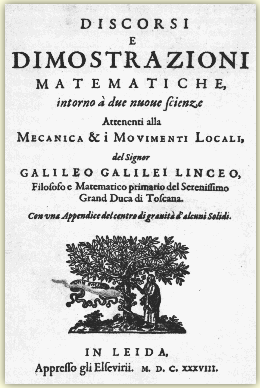
\includegraphics[height=7.5cm,keepaspectratio]{images/frontesp.png}\par
\vfill
{\small\itshape In Leida, Appresso gli Elsevirii\\M. D. C. XXXVIII\par}
\end{titlepage}

% Nota storico-filologica
\chapter*{Nota Storica e Filologica}
\addcontentsline{toc}{chapter}{Nota Storica e Filologica}
\markboth{Nota Storica e Filologica}{Nota Storica e Filologica}

Nel luglio del 1633, a Siena, Galileo comincia a mettere insieme i materiali per la stesura dell'opera. Nel 1635 viene pubblicata a Strasburgo una traduzione in latino dei \emph{Discorsi}, per i tipi di Matthias Bernegger. Nel maggio del 1636 l'editore Louis Elzevier fa visita a Galileo in Arcetri e acconsente alla pubblicazione del saggio in lingua italiana. Tale edizione a stampa vedrà la luce soltanto due anni dopo, nel 1638, a Leida in Olanda.

\vspace{1.5em}
\noindent\textbf{Tavola delle materie principali che si trattano nella presente opera:}
\begin{itemize}
\item[\textbf{I.}] Scienzia nuova prima, intorno alla resistenza de i corpi solidi all'essere spezzati (\emph{Giornata prima}).
\item[\textbf{II.}] Qual potesse esser la causa di tal coerenza (\emph{Giornata seconda}).
\item[\textbf{III.}] Scienzia nuova altra, de i movimenti locali, cioè dell'equabile e del naturalmente accelerato (\emph{Giornata terza}).
\item[\textbf{IV.}] Del violento, o vero de i proietti (\emph{Giornata quarta}).
\item[\textbf{V.}] Appendice di alcune proposizioni e dimostrazioni attenenti al centro di gravità de i solidi.
\end{itemize}

\vfill
\begin{footnotesize}
\noindent\textbf{Nota all'edizione digitale:} Testo conforme all'edizione critica \emph{Opere di Galileo Galilei}, a cura di Franz Brunetti, UTET, Torino 1980 (ISBN 88-02-03457-5), confrontato con l'\emph{Edizione Nazionale delle Opere di Galileo Galilei} a cura di Antonio Favaro (vol.~VIII). Edizione elettronica di riferimento: Progetto Manuzio (a cura di Catia Righi, Giovanni Mazzarello, Claudio Paganelli, Michele Diodati). Riedizione tipografica in \LaTeX{} per uso scientifico e di studio.
\end{footnotesize}

\tableofcontents

% Dedica e Prefazione dello Stampatore
\chapter*{Dedica e Avviso ai Lettori}
\addcontentsline{toc}{chapter}{Allo Illustrissimo Signore il Conte di Noailles}
\markboth{Dedica e Avviso ai Lettori}{Dedica e Avviso ai Lettori}
\section*{Allo Illustrissimo Signore\\il Signore Conte di Noailles}
Consiglier di sua Maestà Cristianissima, Cavalier dell'Ordine di Santo Spirito, Mariscalco de' suoi campi ed esserciti, Siniscalco e Governatore di Roerga e Luogotenente per Sua Maestà in Overgna, mio Signore e Padrone colendissimo.

\emph{Illustrissimo Signore,}

\emph{Riconosco per uno effetto della magnanimità di V. S. Illustrissima quanto gli è piaciuto disporre di questa opera mia; non ostante che (come ella sa), confuso e sbigottito da i mal fortunati successi di altre mie opere, avendo meco medesimo determinato di non esporre in pubblico mai più alcuna delle mie fatiche, ma solo, acciò del tutto non restassero sepolte, essendomi persuaso di lasciarne copia manuscritta in luogo conspicuo al meno a molti intelligenti delle materie da me trattate, e per ciò avendo fatto elezzione, per il primo e più illustre luogo, di depositarle in mano di V. S. Illustrissima, sicuro che, per sua particolare affezzione verso di me, averebbe avuto a cuore la conservazione de' miei studii e fatiche; e per ciò nel suo passaggio di qua, ritornando dalla sua ambasciata di Roma, fui a riverirla personalmente, sì come più volte avevo fatto per lettere; e con tale incontro presentai a V. S. Illustrissima la copia di queste due opere che allora mi trovavo avere in pronto, le quali benignamente mostrò di gradire molto e di essere per farne sicura conserva, e, col participarle in Francia a qualche amico suo, perito di queste scienzie, mostrare che, se bene tacevo, non però passavo la vita del tutto ociosamente. Andavo dipoi apparecchiandomi di mandarne alcune altre copie in Germania, in Fiandra, in Inghilterra, in Spagna, e forse anco in qualche luogo d'Italia, quando improvvisamente vengo da gli Elzevirii avvisato come hanno sotto il torchio queste mie opere, e che però io deva prendere risoluzione circa la dedicatoria e prontamente mandargli il mio concetto sopra di ciò. Mosso da questa inopinata ed inaspettata nuova, sono andato meco medesimo concludendo che la brama di V. S. Illustrissima di suscitare ed ampliare il nome mio, col participare a diversi miei scritti, abbia cagionato che sieno pervenuti nelle mani de' detti stampatori, li quali, essendosi adoperati in publicare altre mie opere, abbiano voluto onorarmi di mandarle alla luce sotto le loro bellissime ed ornatissime stampe. Per ciò questi miei scritti debbono risentirsi per aver avuta la sorte d'andar nell'arbitrio d'un sì gran giudice, il quale, nel maraviglioso concorso di tante virtù che rendono V. S. Illustrissima ammirabile a tutti, ella con incomparabile magnanimità, per zelo anco del ben publico, a cui gli è parso che questa mia opera dovesse conferire, ha voluto allargargli i termini ed i confini dell'onore. Sì che, essendo il fatto ridotto in cotale stato, è ben ragionevole che io con ogni segno più cospicuo mi dimostri grato riconoscitore del generoso affetto di V. S. Illustrissima, che ha avuto a cuore di accrescermi la mia fama con farli spiegar le ale liberamente sotto il cielo aperto, dove che a me pareva assai dono che ella restasse in spazii più angusti. Per tanto al nome vostro, Illustrissimo Signore, conviene che io dedichi e consacri questo mio parto; al che fare mi strigne non solo il cumulo de gli oblighi che gli tengo, ma l'interesse ancora, il quale (siami lecito così dire) mette in obligo V. S. Illustrissima di difendere la mia riputazione contro a chi volesse offenderla, mentre ella mi ha posto in steccato contro a gli avversarii. Onde, facendomi avanti sotto il suo stendardo e protezzione, umilmente me le inchino, con augurarle per premio di queste sue grazie il colmo d'ogni felicità e grandezza.}

D'Arcetri, li 6 Marzo 1638.\\ Di V. S. Illustrissima

Devotissimo Servitore\\ GALILEO GALILEI


\section*{Lo Stampatore a i Lettori}
\addcontentsline{toc}{section}{Lo Stampatore a i Lettori}

Trattenendosi la vita civile mediante il mutuo e vicendevole soccorso de gli uomini gli uni verso gli altri, ed a ciò servendo principalmente l'uso delle arti e delle scienzie, per questo gl'inventori di esse sono sempre stati tenuti in grande stima, e molto riveriti dalla savia antichità; e quanto più eccellente o utile è stata qualche invenzione, tanto maggior laude ed onore ne è stato attribuito a gl'inventori, fin ad essere stati deificati (avendo gli uomini, per commun consenso, con tal segno di supremo onore voluto perpetuare la memoria de gli autori del loro bene essere). Parimente quelli i quali con l'acutezza de i loro ingegni hanno riformato le cose già trovate, scoprendo le fallacie e gli errori di molte e molte proposizioni portate da uomini insigni e ricevute per vere per molte età, sono degni di gran lode ed ammirazione; atteso medesimamente che tale scoprimento è laudabile, se bene i medesimi scopritori avesseno solamente rimossa la falsità, senza introdurne la verità, per sé tanto difficile a conseguirsi, conforme al detto del principe de gli oratori: \emph{Utinam} \emph{tam} \emph{facile} \emph{possem} \emph{vera} \emph{reperire}, \emph{quam} \emph{falsa} \emph{convincere}. Ed in fatti il merito di questa lode è dovuto a questi nostri ultimi secoli, ne i quali le arti e le scienzie, ritrovate da gli antichi, per opera di perspicacissimi ingegni sono, per molte prove ed esperienzie, state ridotte a gran perfezzione, la quale ogni dì va augumentandosi: ed in particolare questo apparisce nelle scienze matematiche, nelle quali (lasciando i diversi che ci si sono adoperati con gran lode e gran successo) al nostro Signore Galileo Galilei, Accademico Linceo, senza alcun contrasto, anzi con l'applauso e l'approbazione universale di tutti i periti, meritamente sono dovuti li primi gradi, sì per aver mostrato la non concludenza di molte ragioni intorno a varie conclusioni, con salde dimostrazioni confermate (come ne sono piene le opere sue già publicate), sì anco per aver col telescopio (uscito prima di queste nostre parti, ma da esso ridotto poi a perfezzione molto maggiore) scoperto e data, primo di tutti, la notizia delle quattro stelle satelliti di Giove, della vera e certa dimostrazione della Via Lattea, delle macchie solari, delle rugosità e parti nebulose della Luna, di Saturno tricorporeo, Venere falcata, della qualità e disposizion delle comete; tutte cose non conosciute mai da gli astronomi né da i filosofi antichi, di maniera che puote dirsi, esser per esso con nuova luce comparsa al mondo e ristorata l'astronomia: dall'eccellenza della quale (in quanto ne' cieli e ne i corpi celesti con maggiore evidenza ed ammirazione che in tutte le altre creature risplende la potenza sapienzia e bontà del supremo Fattore) risulta la grandezza del merito di chi ce ne ha aperta la conoscenza, con aversi resi tali corpi distintamente conspicui, non ostante la loro distanza, quasi infinita, da noi; poi che, secondo il dire volgato, l'aspetto insegna assai più e con maggior certezza in un sol giorno che non potriano fare i precetti, quantunque mille volte reiterati, la notizia intuitiva (come disse un altro) andando del pari con la definizione. Ma molto più si fa manifesta la grazia concedutagli da Dio e dalla natura (per mezzo però di molte fatiche e vigilie) nella presente opera, nella quale si vede, lui essere stato ritrovatore di due intere scienzie nuove, e da i loro primi principii e fondamenti concludentemente, cioè geometricamente, dimostrate: e, quello che deve rendere più maravigliosa questa opera, una delle due scienzie è intorno a un suggetto eterno, principalissimo in natura, speculato da tutti i gran filosofi, e sopra il quale ci sono moltissimi volumi scritti; parlo del moto locale, materia d'infiniti accidenti ammirandi, nessuno de' quali è sin qui stato trovato, non che dimostrato, da alcuno: l'altra scienzia, pure da i suoi principii dimostrata, è intorno alla resistenza che fanno i corpi solidi all'essere per violenza spezzati; notizia di grande utilità, e massime nelle scienzie ed arti mecaniche, ed essa ancora piena d'accidenti e proposizioni sin qui non osservate. Di queste due nuove scienzie, piene di proposizioni che in infinito saranno accresciute col progresso del tempo dagl'ingegni specolativi, in questo libro si aprono le prime porte, e con non piccolo numero di proposizioni dimonstrate si addita il progresso e trapasso ad altre infinite, sì come da gl'intelligenti sarà facilmente inteso e riconosciuto.

\mainmatter

\chapter*{Giornata Prima}
\addcontentsline{toc}{chapter}{Giornata Prima — Intorno alla resistenza de i corpi solidi}
\markboth{Giornata Prima}{Giornata Prima}

\begin{center}
\textbf{Interlocutori:}\\ Salviati, Sagredo e Simplicio
\end{center}

\speaker{Salv.} Largo campo di filosofare a gl'intelletti specolativi parmi che porga la frequente pratica del famoso arsenale di voi, Signori Veneziani, ed in particolare in quella parte che mecanica si domanda; atteso che quivi ogni sorte di strumento e di machina vien continuamente posta da numero grande d'artefici, tra i quali, e per l'osservazioni fatte dai loro antecessori, e per quelle che di propria avvertenza vanno continuamente per se stessi facendo, è forza che ve ne siano de i peritissimi e di finissimo discorso.

\speaker{Sagr.} V. S. non s'inganna punto: ed io, come per natura curioso, frequento per mio diporto la visita di questo luogo e la pratica di questi che noi, per certa preminenza che tengono sopra 'l resto della maestranza, domandiamo proti; la conferenza de i quali mi ha più volte aiutato nell'investigazione della ragione di effetti non solo maravigliosi, ma reconditi ancora e quasi inopinabili. È vero che tal volta anco mi ha messo in confusione ed in disperazione di poter penetrare come possa seguire quello che, lontano da ogni mio concetto, mi dimostra il senso esser vero. E pur quello che poco fa ci diceva quel buon vecchio è un dettato ed una proposizione ben assai vulgata; ma però io la reputava in tutto vana, come molte altre che sono in bocca de i poco intelligenti, credo da loro introdotte per mostrar di saper dir qualche cosa intorno a quello di che non son capaci.

\speaker{Salv.} V. S. vuol forse dire di quell'ultimo pronunziato ch'ei profferì mentre ricercavamo d'intendere per qual ragione facevano tanto maggior apparecchio di sostegni, armamenti ed altri ripari e fortificazioni, intorno a quella gran galeazza che si doveva varare, che non si fa intorno a vasselli minori; dove egli rispose, ciò farsi per evitare il pericolo di direnarsi, oppressa dal gravissimo peso della sua vasta mole, inconveniente al quale non son soggetti i legni minori?

\speaker{Sagr.} Di cotesto intendo, e sopra tutto dell'ultima conclusione ch'ei soggiunse, la quale io ho sempre stimata concetto vano del vulgo; cioè che in queste ed altre simili machine non bisogna argumentare dalle piccole alle grandi, perché molte invenzioni di machine riescono in piccolo, che in grande poi non sussistono. Ma essendo che tutte le ragioni della mecanica hanno i fondamenti loro nella geometria, nella quale non veggo che la grandezza e la piccolezza faccia i cerchi, i triangoli, i cilindri, i coni e qualunque altre figure solide, soggette ad altre passioni queste e ad altre quelle; quando la machina grande sia fabricata in tutti i suoi membri conforme alle proporzioni della minore, che sia valida e resistente all'esercizio al quale ella è destinata, non so vedere perché essa ancora non sia esente da gl'incontri che sopraggiugner gli possono, sinistri e destruttivi.

\speaker{Salv.} Il detto del vulgo è assolutamente vano; e talmente vano, che il suo contrario si potrà profferire con altrettanta verità, dicendo che molte machine si potranno far più perfette in grande che in piccolo: come, per esempio, un oriuolo, che mostri e batta le ore, più giusto si farà d'una tal grandezza che di un'altra minore. Con miglior fondamento usurpano quel medesimo detto altri più intelligenti, i quali della riuscita di tali machine grandi, non conforme a quello che si raccoglie dalle pure ed astratte dimostrazioni geometriche, ne rimettono la causa nell'imperfezzione della materia, che soggiace a molte alterazioni ed imperfezzioni. Ma qui non so s'io potrò, senza inciampare in qualche nota di arroganza, dire che né anco il ricorrere all'imperfezzioni della materia, potenti a contaminare le purissime dimostrazioni matematiche, basti a scusare l'inobbedienza delle machine in concreto alle medesime astratte ed ideali: tuttavia io pure il dirò, affermando che, astraendo tutte l'imperfezzioni della materia e supponendola perfettissima ed inalterabile e da ogni accidental mutazione esente, con tutto ciò il solo esser materiale fa che la machina maggiore, fabbricata dell'istessa materia e con l'istesse proporzioni che la minore, in tutte l'altre condizioni risponderà con giusta simmetria alla minore, fuor che nella robustezza e resistenza contro alle violente invasioni; ma quanto più sarà grande, tanto a proporzione sarà più debole. E perché io suppongo, la materia essere inalterabile, cioè sempre l'istessa, è manifesto che di lei, come di affezzione eterna e necessaria, si possano produr dimostrazioni non meno dell'altre schiette e pure matematiche. Però, Sig. Sagredo, revochi pur l'opinione che teneva, e forse insieme con molti altri che nella mecanica han fatto studio, che le machine e le fabbriche composte delle medesime materie, con puntuale osservanza delle medesime proporzioni tra le loro parti, debban essere egualmente, o, per dir meglio, proporzionalmente, disposte al resistere ed al cedere alle invasioni ed impeti esterni, perché si può geometricamente dimostrare, sempre le maggiori essere a proporzione men resistenti che le minori; sì che ultimamente non solo di tutte le machine e fabbriche artifiziali, ma delle naturali ancora, sia un termine necessariamente ascritto, oltre al quale né l'arte né la natura possa trapassare: trapassar, dico, con osservar sempre l'istesse proporzioni con l'identità della materia.

\speaker{Sagr.} Io già mi sento rivolgere il cervello, e, quasi nugola dal baleno repentinamente aperta, ingombrarmisi la mente da momentanea ed insolita luce, che da lontano mi accenna e subito confonde ed asconde imaginazioni straniere ed indigeste. E da quanto ella ha detto parmi che dovrebbe seguire che fusse impossibil cosa costruire due fabbriche dell'istessa materia simili e diseguali, e tra di loro con egual proporzione resistenti; e quando ciò sia, sarà anco impossibile trovar due sole aste dell'istesso legno tra di loro simili in robustezza e valore, ma diseguali in grandezza.

\speaker{Salv.} Così è, Sig. Sagredo: e per meglio assicurarci che noi convenghiamo nel medesimo concetto, dico che se noi ridurremo un'asta di legno a tal lunghezza e grossezza, che fitta, v. g., in un muro ad angoli retti, cioè parallela all'orizonte, sia ridotta all'ultima lunghezza che si possa reggere, sì che, allungata un pelo più, si spezzasse, gravata dal proprio peso, questa sarà unica al mondo; tal che essendo, per esempio, la sua lunghezza centupla della sua grossezza, nissuna altra asta della medesima materia potrà ritrovarsi che, essendo in lunghezza centupla della sua grossezza, sia, come quella, precisamente abile a sostener se medesima, e nulla di più; ma tutte le maggiori si fiaccheranno, e le minori saranno potenti a sostener, oltre al proprio peso, qualch'altro appresso. E questo che io dico dello stato di regger se medesimo, intendasi detto di ogni altra costituzione; e così se un corrente potrà reggere il peso di dieci correnti suoi eguali, una trave simile a lui non potrà altramente regger il peso di dieci sue eguali. Ma notino in grazia V. S. e 'l Sig. Simplicio nostro, quanto le conclusioni vere, benché nel primo aspetto sembrino improbabili, additate solamente qualche poco, depongono le vesti che le occultavano, e nude e semplici fanno de' lor segreti gioconda mostra. Chi non vede come un cavallo cadendo da un'altezza di tre braccia o quattro si romperà l'ossa, ma un cane da una tale, e un gatto da una di otto o dieci, non si farà mal nissuno, come né un grillo da una torre, né una formica precipitandosi dall'orbe lunare? i piccoli fanciulli restare illesi in cadute, dove i provetti si rompono gli stinchi o la testa? E come gli animali più piccoli sono, a proporzione, più robusti e forti de i maggiori, così le piante minori meglio si sostentano: e già credo che amendue voi apprendiate che una quercia dugento braccia alta non potrebbe sostenere i suoi rami sparsi alla similitudine di una di mediocre grandezza, e che la natura non potrebbe fare un cavallo grande per venti cavalli, né un gigante dieci volte più alto di un uomo, se non o miracolosamente o con l'alterar assai le proporzioni delle membra ed in particolare dell'ossa, ingrossandole molto sopra la simmetria dell'ossa comuni. Il creder parimente che nelle machine artifiziali egualmente siano fattibili e conservabili le grandissime e le piccole, è errore manifesto: e così, per esempio, piccole guglie, colonnette ed altre solide figure, sicuramente si potranno maneggiare distendere e rizzare, senza risico di rompersi, che le grandissime per ogni sinistro accidente andranno in pezzi, e non per altra cagione che per il loro proprio peso. E qui è forza che io vi racconti un caso degno veramente di esser saputo, come sono tutti gli accidenti che accascano fuori dell'aspettazione, e massime quando il partito preso per ovviare a uno inconveniente riesce poi causa potissima del disordine. Era una grossissima colonna di marmo distesa, e posata, presso alle sue estremità, sopra due pezzi di trave; cadde in pensiero dopo certo tempo ad un mecanico che fusse bene, per maggiormente assicurarsi che gravata dal proprio peso non si rompesse nel mezzo, supporgli anco in questa parte un terzo simile sostegno: parve il consiglio generalmente molto opportuno, ma l'esito lo dimostrò essere stato tutto l'opposito, atteso che non passarono molti mesi che la colonna si trovò fessa e rotta, giusto sopra il nuovo appoggio di mezzo.

\speaker{Simp.} Accidente in vero maraviglioso e veramente \emph{praeter spem}, quando però fusse derivato dall'aggiungervi il nuovo sostegno di mezzo.

\speaker{Salv.} Da quello sicuramente derivò egli, e la riconosciuta cagion dell'effetto leva la maraviglia: perché, deposti in piana terra i due pezzi della colonna, si vedde che l'uno de i travi, su 'l quale appoggiava una delle testate, si era, per la lunghezza del tempo, infracidato ed avvallato, e, restando quel di mezzo durissimo e forte, fu causa che la metà della colonna restasse in aria, abbandonata dall'estremo sostegno; onde il proprio soverchio peso gli fece fare quello che non avrebbe fatto se solo sopra i due primi si fusse appoggiata, perché l'avvallarsi qual si fusse di loro, ella ancora l'arebbe seguito. E qui non si può dubitare che tal accidente non sarebbe avvenuto in una piccola colonna, benché della medesima pietra e di lunghezza rispondente alla sua grossezza con la proporzione medesima della grossezza e lunghezza della colonna grande.

\speaker{Sagr.} Già sin qui resto io assicurato della verità dell'effetto ma non penetro già la ragione come, nel crescersi la materia, non deva con l'istesso ragguaglio multiplicarsi la resistenza e gagliardia; e tanto più mi confondo, quanto per l'opposito veggo in altri casi crescersi molto più la robustezza e la resistenza al rompersi, che non cresce l'ingrossamento della materia: che se, v. g., saranno due chiodi fitti in un muro, l'uno più grosso il doppio dell'altro, quello reggerà non solamente doppio peso di questo, ma triplo e quadruplo.

\speaker{Salv.} Dite pur ottuplo, né direte lontano dal vero: né questo effetto contraria a quello, ancor che in sembiante apparisca così diverso.

\speaker{Sagr.} Adunque, Sig. Salviati, spianateci questi scogli e dichiarateci queste oscurità, se ne avete il modo, ché ben conietturo, questa materia delle resistenze essere un campo pieno di belle ed utili contemplazioni; e se vi contentate che questo sia il soggetto de i nostri ragionamenti di oggi, a me, e credo al Sig. Simplicio, sarà gratissimo.

\speaker{Salv.} Non posso mancar di servirle, purché la memoria serva me in sumministrarmi quello che già appresi dal nostro Accademico, che sopra tal materia aveva fatte molte speculazioni, e tutte, conforme al suo solito, geometricamente dimostrate, in modo che, non senza ragione, questa sua potrebbe chiamarsi una nuova scienza; perché se bene alcune delle conclusioni sono state da altri, e prima di tutti da Aristotele, osservate, tuttavia né sono delle più belle, né (quello che più importa) da i loro primarii e indubitati fondamenti con necessarie dimostrazioni provate. E perché, come dico, voglio dimostrativamente accertarvi, e non con solamente probabili discorsi persuadervi, supponendo che abbiate quella cognizione delle conclusioni mecaniche, da altri sin qui fondatamente trattate, che per il nostro bisogno sarà necessaria, conviene che avanti ogni altra cosa consideriamo qual effetto sia quello che si opera nella frazzione di un legno o di altro solido, le cui parti saldamente sono attaccate; perché questa è la prima nozione, nella qual consiste il primo e semplice principio che come notissimo conviene supporsi.


\begin{center}
\begin{center} 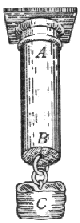
\includegraphics[width=2.00cm,height=5.58cm,keepaspectratio]{images/figura01.png} \end{center}
\end{center}

Per più chiara esplicazione di che, segniamo il cilindro o prisma \emph{AB} di legno o di altra materia solida e coerente, fermato di sopra in \emph{A} e pendente a piombo, al quale nell'altra estremità \emph{B} sia attaccato il peso \emph{C}: è manifesto che, qualunque si sia la tenacità e coerenza tra di loro delle parti di esso solido, pur che non sia infinita, potrà esser superata dalla forza del traente peso \emph{C}, la cui gravità pongo che possa accrescersi quanto ne piace, e esso solido finalmente si strapperà, a guisa d'una corda. E sì come nella corda noi intendiamo, la sua resistenza derivare dalla moltitudine delle fila della canapa che la compongono, così nel legno si scorgono le sue fibre e filamenti distesi per lungo, che lo rendono grandemente più resistente allo strappamento che non sarebbe qualsivoglia canapo della medesima grossezza: ma nel cilindro di pietra o di metallo la coerenza (che ancora par maggiore) delle sue parti depende da altro glutine che da filamenti o fibre; e pure essi ancora da valido tiramento vengono spezzati.

\speaker{Simp.} Se il negozio procede come voi dite, intendo bene che i filamenti nel legno, che son lunghi quanto l'istesso legno, posson renderlo gagliardo e resistente a gran forza che se gli faccia per romperlo; ma una corda composta di fili di canapa non più lunghi di due o tre braccia l'uno, come potrà ridursi alla lunghezza di cento, restando tanto gagliarda? In oltre vorrei anco sentire la vostra opinione intorno all'attaccamento delle parti de i metalli, delle pietre e di altre materie prive di tali filamenti, che pur, s'io non m'inganno, è anco più tenace.

\speaker{Salv.} In nuove specolazioni, e non molto al nostro intento necessarie, converrà divertire, se dovremo delle promosse difficoltà portar le soluzioni.

\speaker{Sagr.} Ma se le digressioni possono arrecarci la cognizione di nuove verità, che pregiudica a noi, non obbligati a un metodo serrato e conciso, ma che solo per proprio gusto facciamo i nostri congressi, digredir ora per non perder quelle notizie che forse, lasciata l'incontrata occasione, un'altra volta non ci si rappresenterebbe? anzi chi sa che bene spesso non si possano scoprir curiosità più belle delle primariamente cercate conclusioni? Pregovi per tanto io ancora a dar sodisfazione al Sig. Simplicio ed a me, non men di esso curioso e desideroso d'intender qual sia quel glutine che sì tenacemente ritien congiunte le parti de i solidi, che pur finalmente sono dissolubili: cognizione che pur anco è necessaria per intender la coerenza delle parti de gli stessi filamenti, de i quali alcuni de i solidi son composti.

\speaker{Salv.} Eccomi a servirvi, poiché così vi piace. È la prima difficoltà, come possano i filamenti d'una corda lunga cento braccia sì saldamente connettersi insieme (non essendo ciascheduno di essi lungo più di due o tre), che gran violenza ci voglia a disseparargli. Ma ditemi, Sig. Simplicio: non potreste voi d'un sol filo di canapa tener l'una dell'estremità talmente stretta fra le dita, che io, tirando dall'altra, prima che liberarlo dalla vostra mano, lo rompessi? Certo sì. Quando dunque i fili della canapa fusser non solo nell'estremità, ma in tutta la lor lunghezza, con gran forza da chi gli circondasse tenuti stretti, non è manifesta cosa che lo sbarbargli da chi gli strigne sarebbe assai più difficile che il rompergli? Ma nella corda l'istesso atto dell'attorcerla strigne le fila scambievolmente tra di loro in maniera, che tirando poi con gran forza la fune, i suoi filamenti si spezzano, e non si separano l'uno dall'altro; come manifestamente si conosce dal vedersi nella rottura i filamenti cortissimi, e non lunghi almeno un braccio l'uno, come dovria vedersi quando la division della corda si facesse non per lo strappamento delle fila, ma per la sola separazione dell'uno dall'altro strisciando.

\speaker{Sagr.} Aggiungasi, in confermazion di questo, il vedersi tal volta romper la corda non per il tirarla per lo lungo, ma solo per il soverchiamente attorcerla: argumento, par a me, concludente, le fila esser talmente tra di loro scambievolmente compresse, che le comprimenti non permettono alle compresse scorrer quel minimo che, che sarebbe necessario per allungar le spire, acciò potessero circondar la fune che nel torcimento si scorcia ed in consequenza qualche poco s'ingrossa.

\speaker{Salv.} Voi benissimo dite: ma considerate appresso come una verità si tira dietro l'altra. Quel filo che stretto tra le dita non segue chi, con qualche forza tirandolo, vorrebbe di tra esse sottrarlo, resiste perché da doppia compressione vien ritenuto; avvenga che non meno il dito superiore preme contro l'inferiore, che questo si prema contro a quello. E non è dubbio che quando di queste due premure se ne potesse ritenere una sola, resterebbe la metà di quella resistenza che dalle due congiunte dependeva; ma perché non si può con l'alzar, v. g., il dito superiore levar la sua pressione senza rimuover anco l'altra parte, conviene con nuovo artifizio conservarne una di loro, e trovar modo che l'istesso filo comprima se medesimo contro al dito o altro corpo solido sopra 'l quale si posa, e far sì che l'istessa forza che lo tira per separarnelo, tanto più ve lo comprima, quanto più gagliardamente lo tira: e questo si conseguirà con l'avvolgere a guisa di spira il filo medesimo intorno al solido; il che acciò meglio s'intenda, ne segnerò un poco di figura.


\begin{center}
\begin{center} 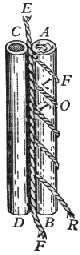
\includegraphics[width=2.00cm,height=6.38cm,keepaspectratio]{images/figura02.png} \end{center}
\end{center}

E questi \emph{AB}, \emph{CD} siano due cilindri, e tra essi disteso il filo \emph{EF}, che per maggior chiarezza ce lo figureremo essere una cordicella: non è dubbio, che premendo gagliardamente i due cilindri l'uno contro all'altro, la corda \emph{FE}, tirata dall'estremità \emph{F}, resisterà a non piccola violenza prima che scorrere tra i due solidi comprimentila; ma se rimuoveremo l'uno di loro, la corda, benché continui di toccar l'altro, non però da tal toccamento sarà ritenuta che liberamente non scorra. Ma se ritenendola, benché debolmente attaccata verso la sommità del cilindro \emph{A}, l'avvolgeremo intorno a quello a foggia di spira \emph{AFLOTR}, e dal capo \emph{R} la tireremo, è manifesto che ella comincerà a stringere il cilindro; e se le spire e volute saranno molte, sempre più, nel validamente tirare, si comprimerà la corda addosso al cilindro; e facendosi, con la multiplicazione delle spire, più lungo il toccamento, ed in consequenza men superabile, difficile si farà sempre più lo scorrer della corda e l'acconsentir alla traente forza. Or chi non vede che tale è la resistenza delle filamenta, che con mille e mille simili avvolgimenti il grosso canapo contessono? Anzi lo strignimento di simili tortuosità collega tanto tenacemente, che di non molti giunchi, né anco molto lunghi, sì che poche son le spire con le quali tra di loro s'intrecciano, si compongono robustissime funi, che mi par che domandino \emph{suste}.

\speaker{Sagr.} Cessa per il vostro discorso nella mia mente la maraviglia di due effetti, de i quali le ragioni non bene erano comprese da me. Uno era il vedere come due o al più tre rivolte del canapo intorno al fuso dell'argano potevano non solamente ritenerlo, che, tirato dall'immensa forza del peso che ei sostiene, scorrendo non gli cedesse, ma che di più, girando l'argano, il medesimo fuso, col solo toccamento del canapo che lo strigne, potesse con li succedenti ravvolgimenti tirare e sollevare vastissime pietre, mentre che le braccia d'un debile ragazzo vanno ritenendo e radunando l'altro capo del medesimo canapo. L'altro è d'un semplice ma arguto ordigno, trovato da un giovane mio parente, per poter con una corda calarsi da una finestra senza scorticarsi crudelmente le palme delle mani, come poco tempo avanti gli era intervenuto con sua grandissima offesa. Ne farò, per facile intelligenza, un piccolo schizzo.


\begin{center}
\begin{center} 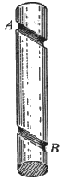
\includegraphics[width=1.50cm,height=4.58cm,keepaspectratio]{images/figura03.png} \end{center}
\end{center}

Intorno a un simil cilindro di legno \emph{AB}, grosso come una canna e lungo circa un palmo, incavò un canaletto in forma di spira, di una voluta e mezo e non più, e di larghezza capace della corda che voleva adoprare; e questa fece entrare per il canale dal termine \emph{A} ed uscire per l'altro \emph{B}, circondando poi tal cilindro e corda con un cannone pur di legno, o vero anco di latta, ma diviso per lungo ed ingangherato, sì che liberamente potesse aprirsi e chiudersi: ed abbracciando poi e strignendo con ambe le mani esso cannone, raccomandata la corda a un fermo ritegno di sopra, si sospese su le braccia; e riuscì tale la compressione della corda tra 'l cannone ambiente e 'l cilindro, che, ad arbitrio suo, strignendo fortemente le mani poteva sostenersi senza calare ed allentandole un poco si calava lentamente a suo piacimento.

\speaker{Salv.} Ingegnosa veramente invenzione; e per intera esplicazione della sua natura, mi par di scorgere così per ombra che qualche altra specolazione si potesse aggiugnere: ma non voglio per ora digredir più sopra di questo particolare, e massime volendo voi sentir il mio pensiero intorno alla resistenza allo strapparsi de gli altri corpi, la cui testura non è di filamenti, come quella delle funi e della maggior parte de i legni; ma la coerenza delle parti loro in altre cagioni par che consista, le quali, per mio giudizio, si riducono a due capi: l'uno de i quali è quella decantata repugnanza che ha la natura all'ammettere il vacuo; per l'altro bisogna (non bastando questo del vacuo) introdur qualche glutine, visco o colla, che tenacemente colleghi le particole delle quali esso corpo è composto. Dirò prima del vacuo, mostrando con chiare esperienze quale e quanta sia la sua virtù. E prima, il vedersi, quando ne piaccia, due piastre di marmo, di metallo o di vetro, esquisitamente spianate pulite e lustre, che, posata l'una su l'altra, senza veruna fatica se gli muove sopra strisciando (sicuro argumento che nissun glutine le congiugne), ma che volendo separarle, mantenendole equidistanti, tal repugnanza si trova, che la superiore solleva e si tira dietro l'altra e perpetuamente la ritiene sollevata, ancorché assai grossa e grave, evidentemente ci mostra l'orrore della natura nel dover ammettere, se ben per breve momento di tempo, lo spazio voto che tra di quelle rimarrebbe avanti che il concorso delle parti dell'aria circostante l'avesse occupato e ripieno. Vedesi anco, che quando bene tali due lastre non fussero esattamente pulite, e perciò che il lor contatto non fusse esquisito del tutto, nel volerle separar lentamente niuna renitenza si trova fuor di quella della sola gravità; ma in un alzamento repentino l'inferior pietra si solleva, ma subito ricade, seguendo solamente la sovrana per quel brevissimo tempo che basta per la distrazzione di quella poca d'aria che s'interponeva tra le lastre, che non ben combaciavano, e per l'ingresso dell'altra circunfusa. Tal resistenza, che così sensatamente si scorge tra le due lastre, non si può dubitare che parimente non risegga tra le parti di un solido, e che nel loro attaccamento non entri almanco a parte e come causa concomitante.

\speaker{Sagr.} Fermate di grazia, e concedetemi ch'io dica una particolar considerazione che pur ora mi è caduta in mente: e questa è, che il vedere come la piastra inferiore segue la superiore e che con moto velocissimo vien sollevata, ci rende sicuri che, contro al detto di molti filosofi e forse d'Aristotele medesimo, il moto nel vacuo non sarebbe instantaneo; perché quando fusse tale, le nominate due lastre senza repugnanza veruna si separerebbero, già che il medesimo instante di tempo basterebbe per la loro separazione e per il concorso dell'aria ambiente a riempier quel vacuo che tra esse potesse restare. Dal seguir dunque che fa l'inferior lastra la superiore, si raccoglie come nel vacuo il moto non sarebbe instantaneo; e si raccoglie insieme che pur tra le medesime piastre resti qualche vacuo, almeno per brevissimo tempo, cioè per tutto quello che passa nel movimento dell'ambiente, mentre concorre a riempiere il vacuo; ché se vacuo non vi restasse, né di concorso né di moto di ambiente vi sarebbe bisogno. Converrà dunque dire che, pur per violenza o contro a natura, il vacuo talor si conceda (benché l'opinion mia è che nissuna cosa sia contro a natura, salvo che l'impossibile, il quale poi non è mai). Ma qui mi nasce un'altra difficoltà; ed è che, se ben l'esperienza m'assicura della verità della conclusione, l'intelletto non resta già interamente appagato della causa alla quale cotale effetto viene attribuito. Imperò che l'effetto della separazione delle due lastre è anteriore al vacuo, che in consequenza alla separazione succederebbe: e perché mi pare che la causa debba, se non di tempo, almeno di natura precedere all'effetto, e che d'un effetto positivo positiva altresì debba esser la causa, non resto capace come dell'aderenza delle due piastre e della repugnanza all'esser separate, effetti che già sono in atto, si possa referir la cagione al vacuo, che non è, ma che arebbe a seguire; e delle cose che non sono, nussuna può esser l'operazione, conforme al pronunziato certissimo del Filosofo.

\speaker{Simp.} Ma già che concedete questo assioma ad Aristotele, non credo che siate per negargliene un altro, bellissimo e vero: e questo è, che la natura non intraprende a voler fare quello che repugna ad esser fatto, dal qual pronunziato mi par che dependa la soluzione del vostro dubbio. Perché dunque a se medesimo repugna essere uno spazio vacuo, vieta la natura il far quello in consequenza di che necessariamente succederebbe il vacuo; e tale è la separazione delle due lastre.

\speaker{Sagr.} Ora, ammesso per soluzione adequata del mio dubbio questo che produce il Sig. Simplicio, seguitando il cominciato discorso, parmi che questa medesima repugnanza al vacuo devrebbe esser bastante ritegno delle parti di un solido di pietra o di metallo, o se altre ve ne sono che più saldamente stiano congiunte e renitenti alla divisione. Perché, se di uno effetto una sola è la cagione, sì come io ho inteso e creduto, o, se pur molte se n'assegnano, ad una sola si riducono, perché questa del vacuo, che sicuramente è, non basterà per tutte le resistenze?

\speaker{Salv.} Io per ora non voglio entrare in questa contesa, se il vacuo senz'altro ritegno sia per sé solo bastante a tenere unite le parti disunibili de i corpi consistenti; ma vi dico bene che la ragione del vacuo, che milita e conclude nelle due piastre, non basta per sé sola al saldo collegamento delle parti di un solido cilindro di marmo o di metallo, le quali, violentate da forze gagliarde che dirittamente le tirino, finalmente si separano e si dividono. E quando io trovi modo di distinguer questa già conosciuta resistenza, dependente dal vacuo, da ogni altra, qualunque ella si fusse, che con lei concorresse in fortificar l'attaccamento, e che io vi faccia vedere come essa sola non sia a gran pezzo bastante per tale effetto, non concederete voi che sia necessario introdurne altra? Aiutatelo, Sig. Simplicio, già che egli sta ambiguo sopra quello che debba rispondere.

\speaker{Simp.} È forza che la sospensione del Sig. Sagredo sia per altro rispetto, non restando luogo di dubitare sopra sì chiara e necessaria consequenza.

\speaker{Sagr.} Voi, Sig. Simplicio, l'avete indovinata. Andavo pensando se, non bastando un million d'oro l'anno, che vien di Spagna, per pagar l'esercito, fusse necessario far altra provisione che di danari per le paghe de' soldati. Ma seguitate pur, Sig. Salviati, e supponendo ch'io ammetta la vostra consequenza, mostrateci il modo di separare l'operazione del vacuo dall'altre, e misurandola fateci vedere come ella sia scarsa per l'effetto di che si parla.

\speaker{Salv.} Il vostro demonio vi assiste. Dirò il modo dell'appartar la virtù del vacuo dall'altre, e poi la maniera del misurarla. E per appartarla, piglieremo una materia continua, le cui parti manchino di ogni altra resistenza alla separazione fuor che di quella del vacuo, quale a lungo è stato dimostrato in certo trattato del nostro Accademico esser l'acqua: talché, qualunque volta si disponesse un cilindro d'acqua, e che, attratto, si sentisse resistenza allo staccamento delle sue parti, questo da altra cagione che dalla repugnanza al vacuo non potrebbe riconoscersi. Per far poi una tale esperienza mi son immaginato un artifizio, il quale con l'aiuto di un poco di disegno, meglio che con semplici parole, potrò dichiarare.


\begin{center}
\begin{center} 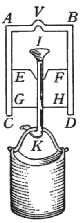
\includegraphics[width=2.00cm,height=5.58cm,keepaspectratio]{images/figura04.png} \end{center}
\end{center}

Figuro, questo \emph{CABD} essere il profilo di un cilindro di metallo o di vetro, che sarebbe meglio, voto dentro, ma giustissimamente tornito, nel cui concavo entri con esquisitissimo contatto un cilindro di legno, il cui profilo noto \emph{EGHF}, il qual cilindro si possa spignere in su e 'n giù; e questo voglio che sia bucato nel mezzo, sì che vi passi un filo di ferro, oncinato nell'estremità \emph{K}, e l'altro capo \emph{I} vadia ingrossandosi in forma di cono o turbine, facendo che il foro fatto nel legno sia nella parte di sopra esso ancora incavato in forma di conica superficie, aggiustata puntualmente per ricevere la conica estremità \emph{I} del ferro \emph{IK}, qualunque volta si tiri giù dalla parte \emph{K}. Inserto il legno, o vogliamolo chiamar zaffo, \emph{EH} nel cavo cilindro \emph{AD}, non voglio ch'arrivi sino alla superior superficie di esso cilindro, ma che resti lontano due o tre dita; e tale spazio deve esser ripieno di acqua, la quale vi si metterà tenendo il vaso con la bocca \emph{CD} all'in su e calcandovi sopra il zaffo \emph{EH}, col tenere il turbine \emph{I} remoto alquanto dal cavo del legno per lasciar l'esito all'aria, che nel calcare il zaffo se n'uscirà per il foro del legno, che perciò si fa alquanto più largo della grossezza dell'asticciuola di ferro \emph{IK}. Dato l'esito all'aria e ritirato il ferro, che ben suggelli su 'legno col suo turbine \emph{I}, si rivolterà il vaso tutto con la bocca all'in giù, ed attaccando all'oncino \emph{K} un recipiente da mettervi dentro rena o altra materia grave, si caricherà tanto, che finalmente la superior superficie \emph{EF} del zaffo si staccherà dall'inferiore dell'acqua, alla quale niente altro la teneva congiunta che la repugnanza del vacuo; pesando poi il zaffo col ferro col recipiente e con ciò che vi sarà dentro, aremo la quantità della forza del vacuo: e se, attaccato a un cilindro di marmo o di cristallo, grosso quanto il cilindro dell'acqua, peso tale che, insieme col peso proprio dell'istesso marmo o cristallo, pareggi la gravità di tutte le nominate bagaglie, ne seguirà la rottura, potremo senza verun dubbio affermare, la sola ragion del vacuo tener le parti del marmo e cristallo congiunte; ma non bastando, e che per romperlo bisogni aggiugnervi quattro volte altrettanto peso, converrà dire, la resistenza del vacuo esser delle cinque parti una, e l'altra quadrupla di quella del vacuo.

\speaker{Simp.} Non si può negare che l'invenzione non sia ingegnosa, ma l'ho per soggetta a molte difficoltà, che me la rendono dubbia: perché, chi ci assicura che l'aria non possa penetrar tra 'l vetro e 'l zaffo, ancorché si circondi bene di stoppa o altra materia cedente? e così, acciò che il cono \emph{I} saldi bene il foro, forse non basterebbe l'ugnerlo con cera o trementina. In oltre, perché non potrebbero le parti dell'acqua distrarsi e rarefarsi? perché non penetrare aria, o esalazioni, o altre sustanze più sottili, per le porosità del legno, o anche dell'istesso vetro?

\speaker{Salv.} Molto destramente ci muove il Sig. Semplicio le difficoltà, ed in parte ci sumministra i rimedii, quanto alla penetrazion dell'aria per il legno, o tra 'l legno e 'l vetro. Ma io, oltre di ciò, noto che potremo nell'istesso tempo accorgerci, con acquisto di nuove cognizioni, se le promosse difficoltà aranno luogo. Imperò che, se l'acqua sarà per natura, se ben con violenza, distraibile, come accade nell'aria, si vedrà il zaffo calare; e se faremo nella parte superiore del vetro un poco di ombelico prominente, come questo \emph{V}, penetrando, per la sustanza o porosità del vetro o del legno, aria o altra più tenue e spiritosa materia, si vedrà radunare (cedendogli l'acqua) nell'eminenza \emph{V}: le quali cose quando non si scorgano, verremo assicurati, l'esperienza esser con le debite cautele stata tentata; e conosceremo, l'acqua non esser distraibile, né il vetro esser permeabile da veruna materia, benché sottilissima.

\speaker{Sagr.} Ed io mercé di questi discorsi ritrovo la causa di un effetto che lungo tempo m'ha tenuto la mente ingombrata di maraviglia e vota d'intelligenza. Osservai già una citerna, nella quale, per trarne l'acqua, fu fatta fare una tromba, da chi forse credeva, ma vanamente, di poterne cavar con minor fatica l'istessa o maggior quantità che con le secchie ordinarie; ed ha questa tromba il suo stantuffo e animella su alta, sì che l'acqua si fa salire per attrazzione, e non per impulso, come fanno le trombe che hanno l'ordigno da basso. Questa, sin che nella citerna vi è acqua sino ad una determinata altezza, la tira abbondantemente; ma quando l'acqua abbassa oltre a un determinato segno, la tromba non lavora più. Io credetti, la prima volta che osservai tale accidente, che l'ordigno fusse guasto; e trovato il maestro acciò lo raccomodasse, mi disse che non vi era altrimente difetto alcuno, fuor che nell'acqua, la quale, essendosi abbassata troppo, non pativa d'esser alzata a tanta altezza; e mi soggiunse, né con trombe, né con altra machina che sollevi l'acqua per attrazzione, esser possibile farla montare un capello più di diciotto braccia: e siano le trombe larghe o strette, questa è la misura dell'altezza limitatissima. Ed io sin ora sono stato così poco accorto, che, intendendo che una corda, una mazza di legno e una verga di ferro, si può tanto e tanto allungare che finalmente il suo proprio peso la strappi, tenendola attaccata in alto, non mi è sovvenuto che l'istesso, molto più agevolmente, accaderà di una corda o verga di acqua. E che altro è quello che si attrae nella tromba, che un cilindro di acqua, il quale, avendo la sua attaccatura di sopra, allungato più e più, finalmente arriva a quel termine oltre al quale, tirato dal suo già fatto soverchio peso, non altrimente che se fusse una corda, si strappa?

\speaker{Salv.} Così puntualmente cammina il negozio; e perché la medesima altezza delle diciotto braccia è il prefisso termine dell'altezza alla quale qualsivoglia quantità d'acqua, siano cioè le trombe larghissime o strette o strettissime quanto un fil di paglia, può sostentarsi, tutta volta che noi peseremo l'acqua contenuta in diciotto braccia di cannone, sia largo o stretto, aremo il valore della resistenza del vacuo ne i cilindri di qualsivoglia materia solida, grossi quanto sono i concavi de i cannoni proposti. E già che aviamo detto tanto, mostriamo come di tutti i metalli, pietre, legni, vetri, etc., si può facilmente ritrovare sino a quanta lunghezza si potrebbono allungare cilindri, fili o verghe di qualsivoglia grossezza, oltre alla quale, gravati dal proprio peso, più non potrebber reggersi, ma si strapperebbero. Piglisi, per esempio, un fil di rame di qualsivoglia grossezza e lunghezza, e fermato un de' suoi capi ad alto, si vadia aggiungendo all'altro maggior e maggior peso, sì che finalmente si strappi; e sia il peso massimo che potesse sostenere, v. g., cinquanta libbre: è manifesto che cinquanta libbre di rame, oltre al proprio peso, che sia, per esempio, un ottavo d'oncia, tirato in filo di tal grossezza, sarebbe la lunghezza massima del filo che se stesso potesse reggere. Misurisi poi quanto era lungo il filo che si strappò, e sia, v. g., un braccio: e perché pesò un ottavo d'oncia, e resse se stesso e cinquanta libbre appresso, che sono ottavi d'oncia quattro mila ottocento, diremo, tutti i fili di rame, qualunque si sia la loro grossezza, potersi reggere sino alla lunghezza di quattro mila ottocento un braccio, e non più. E così, una verga di rame potendo reggersi sino alla lunghezza di quattro mila ottocento un braccio, la resistenza che ella trova dependente dal vacuo, rispetto al restante, è tanta, quanto importa il peso d'una verga d'acqua lunga braccia diciotto e grossa quanto quella stessa di rame; e trovandosi, v. g., il rame esser nove volte più grave dell'acqua, di qualunque verga di rame la resistenza allo strapparsi, dependente dalla ragion del vacuo, importa quanto è il peso di due braccia dell'istessa verga. E con simil discorso ed operazione si potranno trovare le lunghezze delle fila o verghe di tutte le materie solide ridotte alla massima che sostener si possa, ed insieme qual parte abbia il vacuo della loro resistenza.

\speaker{Sagr.} Resta ora che ci dichiate in qual cosa consista il resto della resistenza, cioè qual sia il glutine o visco che ritien attaccate le parti del solido, oltre a quello che deriva dal vacuo: perché io non saprei imaginarmi qual colla sia quella che non possa esser arsa e consumata dentro una ardentissima fornace in due, tre e quattro mesi, né in dieci o in cento; dove stando tanto tempo argento oro e vetro liquefatti, cavati, poi tornano le parti loro, nel freddarsi, a riunirsi e rattaccarsi come prima. Oltre che, la medesima difficoltà che ho nell'attaccamento delle parti del vetro, l'arò io nelle parti della colla, cioè che cosa sia quella che le tiene così saldamente congiunte.

\speaker{Salv.} Pur poco fa vi dissi che 'l vostro demonio vi assisteva. Sono io ancora nelle medesime angustie; ed ancor io, toccando con mano come la repugnanza al vacuo è indubitabilmente quella che non permette, se non con gran violenza, la separazione delle due lastre, e più delle due gran parti della colonna di marmo o di bronzo, non so vedere come non abbia ad aver luogo ed esser parimente cagione della coerenza delle parti minori e sino delle minime ultime delle medesime materie: ed essendo che d'un effetto una sola è la vera e potissima causa, mentre io non trovo altro glutine, perché non debbo tentar di vedere se questo del vacuo, che si trova, può bastarci?

\speaker{Simp.} Se di già voi avete dimostrato, la resistenza del gran vacuo, nel separarsi le due gran parti di un solido, esser piccolissima in comparazion di quella che tien congiunte le particole minime, come non volete tener più che per certo, questa esser diversissima da quella?

\speaker{Salv.} A questo rispose il Sig. Sagredo, che pur si pagavano tutti i particolari soldati con danari raccolti da imposizioni generali di soldi e di quattrini, se bene un million d'oro non bastava a pagar tutto l'esercito. E chi sa che altri minutissimi vacui non lavorino per le minutissime particole, sì che per tutto sia dell'istessa moneta quello con che si tengono tutte le parti congiunte? Io vi dirò quello che tal ora mi è passato per l'imaginazione, e ve lo do non come verità risoluta, ma come una qual si sia fantasia, piena anco d'indigestioni, sottoponendola a più alte contemplazioni: cavatene se nulla vi è che vi gusti; il resto giudicatelo come più vi pare. Nel considerar tal volta come, andando il fuoco serpendo tra le minime particole di questo e di quel metallo, che tanto saldamente si trovano congiunte, finalmente le separa e disunisce; e come poi, partendosi il fuoco, tornano con la medesima tenacità di prima a ricongiugnersi, senza diminuirsi punto la quantità nell'oro, e pochissimo in altri metalli, anco per lungo tempo che restino distrutti; pensai che ciò potesse accadere perché le sottilissime particole del fuoco, penetrando per gli angusti pori del metallo (tra i quali, per la loro strettezza, non potessero passare i minimi dell'aria né di molti altri fluidi), col riempiere i minimi vacui tra esse fraposti liberassero le minime particole di quello dalla violenza con la quale i medesimi vacui l'una contro l'altra attraggono, proibendogli la separazione; e così, potendosi liberamente muovere, la lor massa ne divenisse fluida, e tale restasse sin che gl'ignicoli tra esse dimorassero; partendosi poi quelli e lasciando i pristini vacui, tornasse la lor solita attrazzione, ed in consequenza l'attaccamento delle parti. Ed all'istanza del Sig. Simplicio parmi che si possa rispondere, che se bene tali vacui sarebber piccolissimi, ed in consequenza ciascheduno facile ad esser superato, tuttavia l'innumerabile moltitudine innumerabilmente (per così dire) multiplica le resistenze: e quale e quanta sia la forza che da numero immenso di debolissimi momenti insieme congiunti risulta, porgacene evidentissimo argomento il veder noi un peso di milioni di libbre, sostenuto da canapi grossissimi, cedere e finalmente lasciarsi vincere e sollevare dall'assalto de gl'innumerabili atomi di acqua, li quali, o spinti dall'austro, o pur che, distesi in tenuissima nebbia, si vadano movendo per l'aria, vanno a cacciarsi tra fibra e fibra de i canapi tiratissimi, né può l'immensa forza del pendente peso vietargli l'entrata; sì che, penetrando per gli angusti meati, ingrossano le corde e per consequenza le scorciano, onde la mole gravissima a forza vien sollevata.

\speaker{Sagr.} Ei non è dubbio alcuno che mentre una resistenza non sia infinita, può dalla moltitudine di minimissime forze esser superata, sì che anco un numero di formiche stracicherebbe per terra una nave carica di grano; perché il senso ci mostra cotidianamente che una formica destramente porta un granello, e chiara cosa è che nella nave non sono infiniti granelli, ma compresi dentro a qualche numero, del quale se ne può prendere un altro quattro e sei volte maggiore, al quale se se ne prenderà un altro di formiche eguale, e si porranno in opera, condurranno per terra il grano e la nave ancora. È ben vero che bisognerà che il numero sia grande, come anco, per mio parere, quello de i vacui che tengono attaccati i minimi del metallo.

\speaker{Salv.} Ma quando bisognasse che fussero anche infiniti, l'avete voi forse per impossibile?

\speaker{Sagr.} No, quando quel metallo fusse una mole infinita: altrimenti...

\speaker{Salv.} Altrimenti che? Orsù, già che si è messo mano a i paradossi, veggiamo se in qualche maniera si potesse dimostrare, come in una continua estensione finita non repugni il potersi ritrovar infiniti vacui; e nell'istesso tempo ci verrà, se non altro, almeno arrecata una soluzione del più ammirabil problema che sia da Aristotele messo tra quelli che esso medesimo addimanda ammirandi, dico tra le questioni mecaniche; e la soluzione potrebbe esser per avventura non meno esplicante e concludente di quella che egli medesimo ne arreca, e diversa anco da quello che molto acutamente vi considera il dottissimo Monsig. di Guevara. Ma bisogna prima dichiarare una proposizione non toccata da altri, dalla quale depende lo scioglimento della questione, che poi, s'io non m'inganno, si tira dietro altre notizie nuove ed ammirande: per intelligenza di che, accuratamente descriveremo la figura.


\begin{center}
\begin{center} 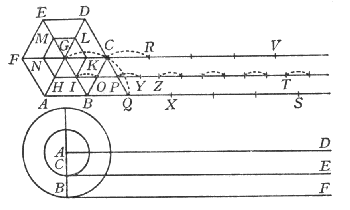
\includegraphics[width=8.75cm,height=5.25cm,keepaspectratio]{images/figura05.png} \end{center}
\end{center}

Però intendiamo un poligono equilatero ed equiangolo, di quanti lati esser si voglia, descritto intorno a questo centro \emph{G}, e sia per ora un esagono \emph{ABCDEF}; simile al quale, e ad esso concentrico, ne descriveremo un altro minore, quale noteremo \emph{HIKLMN}: e del maggiore si prolunghi un lato \emph{AB} indeterminatamente verso \emph{S}, e del minore il rispondente lato \emph{HI} sia verso la medesima parte similmente prodotto, segnando la linea \emph{HT} parallela all'\emph{AS}, e per il centro passi l'altra, alle medesime equidistante, \emph{GV}. Fatto questo, intendiamo il maggior poligono rivolgersi sopra la linea \emph{AS}, portando seco l'altro poligono minore. È chiaro che, stando fisso il punto \emph{B}, termine del lato \emph{AB}, mentre si comincia la revoluzione, l'angolo \emph{A} si solleverà, e 'l punto \emph{C} s'abbasserà descrivendo l'arco \emph{CQ}, sì che il lato \emph{BC} si adatti alla linea a se stesso eguale \emph{BQ}: ma in tal conversione l'angolo \emph{I} del minor poligono si eleverà sopra la linea \emph{IT}, per esser la \emph{IB} obliqua sopra l'\emph{AS}, né prima tornerà il punto \emph{I} su la parallela \emph{IT}, se non quando il punto \emph{C} sarà pervenuto in \emph{Q}; allora l'\emph{I} sarà caduto in \emph{O}, dopo aver descritto l'arco \emph{IO} fuori della linea \emph{HT}, ed allora il lato \emph{IK} sarà passato in \emph{OP}: ma il centro \emph{G} tra tanto sempre averà caminato fuori della linea \emph{GV}, su la quale non sarà tornato se non dopo aver descritto l'arco \emph{GC}. Fatto questo primo passo, il poligono maggiore sarà trasferito a posare co 'l lato \emph{BC} su la linea \emph{BQ}, il lato \emph{IK} del minore sopra la linea \emph{OP}, avendo saltato tutta la parte \emph{IO} senza toccarla, e 'l centro \emph{G} pervenuto in \emph{C}, facendo tutto il suo corso fuori della parallela \emph{GV}, e finalmente tutta la figura si sarà rimessa in un posto simile al primo: sì che continuandosi la revoluzione e venendo al secondo passo, il lato del maggior poligono \emph{CD} si adatterà alla parte \emph{QX}, il \emph{KL} del minore (avendo prima saltato l'arco \emph{PY}) caderà in \emph{YZ}, ed il centro, procedendo sempre fuori della \emph{GV}, in essa caderà solamente in \emph{R}, dopo il gran salto \emph{CR}: ed in ultimo, finita una intera conversione, il maggior poligono avrà calcate sopra la sua \emph{AS} sei linee eguali al suo perimetro, senza veruna interposizione; il poligono minore arà parimente impresse sei linee eguali all'ambito suo, ma discontinuate dall'interposizione de' cinque archi, sotto i quali restano le corde, parti della parallela \emph{HT}, non tocche dal poligono; e finalmente il centro \emph{G} non è convenuto mai con la parallela \emph{GV}, salvo che in sei punti. Di qui potete comprendere come lo spazio passato dal minor poligono è quasi eguale al passato del maggiore, cioè la linea \emph{HT} alla \emph{AS}, della quale è solamente minore quanto è la corda d'uno di questi archi, intendendo però la linea \emph{HT} insieme con li spazii de i cinque archi. Ora questo, che vi ho esposto e dichiarato nell'esempio di questi essagoni, vorrei che intendeste accadere di tutti gli altri poligoni, di quanti lati esser si voglino, purché siano simili, concentrici e congiunti, e che alla conversion del maggiore s'intenda rigirarsi anco l'altro, quanto si voglia minore; che intendeste, dico, le linee da essi passate esser prossimamente eguali, computando nello spazio passato dal minore gl'intervalli sotto gli archetti, non tocchi da parte veruna del perimetro di esso minor poligono. Passa dunque il gran poligono di mille lati, e misura consequentemente, una linea retta eguale al suo ambito; e nell'istesso tempo il piccolo passa una prossimamente egual linea, ma interrottamente composta di mille particelle eguali a i suoi mille lati con l'interposizione di mille spazii vacui, che tali possiamo chiamargli in relazione alle mille lineette toccate da i lati del poligono: ed il detto sin qui non ha veruna difficoltà o dubitazione. Ma ditemi: se intorno a un centro, qual sia, v. g., questo punto \emph{A}, noi descriveremo due cerchi concentrici ed insieme uniti, e che da i punti \emph{C}, \emph{B} de i lor semidiametri siano tirate le tangenti \emph{CE}, \emph{BF}, e ad esse per il centro \emph{A} la parallela \emph{AD}, intendendo girato il cerchio maggiore sopra la linea \emph{BF} (posta eguale alla di lui circonferenza, come parimente le altre due \emph{CE}, \emph{AD}), compita che abbia una revoluzione, che averà fatto il minor cerchio, e che il centro? Questo sicuramente averà scorsa e toccata tutta la linea \emph{AD}, e la circonferenza di quello averà con li suoi toccamenti misurata tutta la \emph{CE}, facendo l'istesso che fecero i poligoni di sopra: in questo solamente differenti, che la linea \emph{HT} non fu tocca in tutte le sue parti del perimetro del minor poligono, ma ne furon lasciate tante intatte, con l'interposizione de' vacui saltati, quante furon le parti tocche da i lati; ma qui ne i cerchi mai non si separa la circonferenza del minor cerchio della linea \emph{CE}, sì che alcuna sua parte non venga tocca, né mai quello che tocca della circonferenza è manco del toccato nella retta. Or come dunque può senza salti scorrere il cerchio minore una linea tanto maggiore della sua circonferenza?

\speaker{Sagr.} Andava pensando se si potesse dire, che sì come il centro del cerchio, esso solo, stracicato copra \emph{AD}, la tocca tutta, essendo anco un punto solo, così potessero i punti della circonferenza minore, tirati dal moto della maggiore, andare strascicandosi per qualche particella della linea \emph{CE}.

\speaker{Salv.} Questo non può essere, per due ragioni. Prima, perché non sarebbe maggior ragione che alcuno de i toccamenti simili al \emph{C} andassero stracicando per qualche parte della linea \emph{CE}, ed altri no; e quando questo fusse, essendo tali toccamenti (perché son punti) infiniti, gli strascichi sopra la \emph{CE} sarebbero infiniti, ed essendo quanti, farebbero una linea infinita; ma la \emph{CE} è finita. L'altra ragione è, che mutando il cerchio grande, nella sua conversione, continuamente contatto, non può non mutarlo parimente il minor cerchio, non si potendo da altro punto che dal punto \emph{B} tirare una linea retta sino al centro \emph{A} e che passasse per il punto \emph{C}; sì che mutando contatto la circonferenza grande, lo muta ancora la piccola, né punto alcuno della piccola tocca più d'un punto della sua retta \emph{CE}. Oltre che, anco nella conversione de i poligoni nissun punto del perimetro del minore si adattava a più d'un punto della linea che dal medesimo perimetro veniva misurata; come si può facilmente intendere considerando la linea \emph{IK} esser parallela alla \emph{BC}, onde sin che la \emph{BC} non si schiaccia sopra la \emph{BQ}, la \emph{IK} resta sollevata sopra la \emph{IP}, né prima la calca se non nel medesimo instante che la \emph{BC} si unisce con la \emph{BQ}, ed allora tutta insieme la \emph{IK} si unisce con la \emph{OP}, e poi immediatamente se gli eleva sopra.

\speaker{Sagr.} Il negozio è veramente molto intrigato, né a me sovviene scioglimento alcuno: però diteci quello che a voi sovviene.

\speaker{Salv.} Io ricorrerei alla considerazione de i poligoni sopra considerati, l'effetto de i quali è intelligibile e di già compreso: e direi, che sì come ne i poligoni di cento mila lati alla linea passata e misurata dal perimetro del maggiore, cioè da i cento mila suoi lati continuamente distesi, è eguale la misurata da i cento mila lati del minore, ma con l'interposizione di cento mila spazii vacui traposti; così direi, ne i cerchi (che son poligoni di lati infiniti) la linea passata da gl'infiniti lati del cerchio grande, continuamente disposti, esser pareggiata in lunghezza dalla linea passata da gl'infiniti lati del minore, ma da questi con l'interposizion d'altrettanti vacui tra essi; e sì come i lati non son quanti, ma bene infiniti, così gl'interposti vacui non son quanti, ma infiniti: quelli, cioè, infiniti punti tutti pieni; e questi, infiniti punti parte pieni e parte vacui. E qui voglio che notiate, come risolvendo e dividendo una linea in parti quante, e per consequenza numerate, non è possibile disporle in una estensione maggiore di quella che occupavan mentre stavano continuate e congiunte senza l'interposizione d'altrettanti spazii vacui; ma imaginandola risoluta in parti non quante, cioè ne' suoi infiniti indivisibili, la possiamo concepire distratta in immenso senza l'interposizione di spazii quanti vacui, ma sì bene d'infiniti indivisibili vacui. E questo, che si dice delle semplici linee, s'intenderà detto delle superficie e de' corpi solidi, considerandogli composti di infiniti atomi non quanti: che mentre gli vorremo dividere in parti quante, non è dubbio che non potremo disporle in spazii più ampli del primo occupato dal solido se non con l'interposizione di spazii quanti vacui, vacui, dico, almeno della materia del solido; ma se intenderemo l'altissima ed ultima resoluzione fatta ne i primi componenti non quanti ed infiniti potremo concepire tali componenti distratti in spazio immenso senza l'interposizione di spazii quanti vacui, ma solamente di vacui infiniti non quanti: ed in questa guisa non repugna distrarsi, v. g., un piccolo globetto d'oro in uno spazio grandissimo senza ammettere spazii quanti vacui; tutta volta però che ammettiamo, l'oro esser composto di infiniti indivisibili.

\speaker{Simp.} Parmi che voi caminiate alla via di quei vacui disseminati di certo filosofo antico.

\speaker{Salv.} Ma però voi non soggiugnete «il quale negava la Providenza divina», come in certo simil proposito, assai poco a proposito, soggiunse un tale antagonista del nostro Accademico.

\speaker{Simp.} Veddi bene, e non senza stomaco, il livore del mal affetto contradittore: ma io non solamente per termine di buona creanza non toccherei simili tasti, ma perché so quanto sono discordi dalla mente ben temperata e bene organizzata di V. S., non solo religiosa e pia, ma cattolica e santa. Ma ritornando su 'l proposito, molte difficoltà sento nascermi da gli auti discorsi, dalle quali veramente io non saprei liberarmi. E per una mi si para avanti questa, che se le circonferenze de i due cerchi sono eguali alle due rette \emph{CE}, \emph{BF}, questa continuamente presa, e quella con l'interposizione d'infiniti punti vacui, l'\emph{AD} descritta dal centro, che è un punto solo, in qual maniera si potrà chiamare ad esso eguale, contenendone infiniti? In oltre, quel comporre la linea di punti, il divisibile di indivisibili, il quanto di non quanti, mi paiono scogli assai duri da passargli e l'istesso dover ammettere il vacuo, tanto concludentemente reprovato da Aristotele, non manca delle medesime difficoltà.

\speaker{Salv.} Ci sono veramente coteste, e dell'altre: ma ricordiamoci che siamo tra gl'infiniti e gl'indivisibili, quelli incomprensibili dal nostro intelletto finito per la lor grandezza, e questi per la lor piccolezza. Con tutto ciò veggiamo che l'umano discorso non vuol rimanersi dall'aggirarsegli attorno; dal che pigliando io ancora qualche libertà, produrrei alcuna mia fantasticheria, se non concludente necessariamente, almeno, per la novità, apportatrice di qualche maraviglia. Ma forse il divertir tanto lungamente dal cominciato cammino potrebbe parervi importuno, e però poco grato.

\speaker{Sagr.} Di grazia, godiamo del benefizio e privilegio che s'ha dal parlar con i vivi e tra gli amici, e più di cose arbitrarie e non necessarie, differente dal trattar co' i libri morti, li quali ti eccitano mille dubbi e nissuno te ne risolvono. Fateci dunque partecipi di quelle considerazioni che il corso de i nostri ragionamenti vi suggerisce, ché non ci mancherà tempo, mercé dell'esser noi disobbligati da funzioni necessarie, di continuar e risolvere l'altre materie intraprese; ed in particolare i dubbii toccati dal Sig. Simplicio non si trapassino in tutti i modi.

\speaker{Salv.} Così si faccia, poiché tale è il vostro gusto: e cominciando dal primo, che fu come si possa mai capire che un sol punto sia eguale ad una linea, vedendo di non ci poter far altro per ora, procurerò di quietare o almeno temperare una improbabilità con un'altra simile o maggiore, come talvolta una maraviglia si attutisce con un miracolo. E questo sarà col mostrarvi, due superficie eguali, ed insieme due corpi pur eguali e sopra le medesime dette superficie, come basi loro, collocati, andarsi continuamente ed egualmente, e queste e quelli, nel medesimo tempo diminuendo, restando sempre tra di loro eguali i loro residui, e finalmente andare, sì le superficie come i solidi, a terminare le lor perpetue egualità precedenti, l'uno de i solidi con l'una delle superficie in una lunghissima linea, e l'altro solido con l'altra superficie in un sol punto, cioè, questi in un sol punto, e quelli in infiniti.

\speaker{Sagr.} Ammirabil proposta veramente mi par cotesta; però sentiamone l'esplicazione e la dimostrazione.

\speaker{Salv.} È necessario farne la figura, perché la prova è pura geometrica.


\begin{center}
\begin{center} 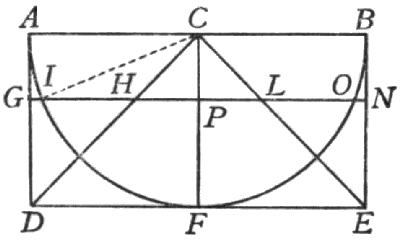
\includegraphics[width=10.00cm,height=6.05cm,keepaspectratio]{images/figura06.png} \end{center}
\end{center}

Per tanto intendasi il mezzo cerchio \emph{AFB}, il cui centro \emph{C}, ed intorno ad esso il parallellogrammo rettangolo \emph{ADEB}, e dal centro a i punti \emph{D}, \emph{E} siano tirate le rette linee \emph{CD}, \emph{CE}; figurandoci poi il semidiametro \emph{CF}, perpendicolare a una delle due \emph{AB}, \emph{DE}, immobile, intendiamo intorno a quello girarsi tutta questa figura: è manifesto che dal rettangolo \emph{ADEB} verrà descritto un cilindro, dal semicircolo \emph{AFB} una mezza sfera, e dal triangolo \emph{CDE} un cono. Inteso questo, voglio che ci immaginiamo esser levato via l'emisferio, lasciando però il cono e quello che rimarrà del cilindro, il quale, dalla figura che riterrà simile a una scodella, chiameremo pure scodella: della quale e del cono prima dimostreremo che sono eguali; e poi, un piano tirato parallelo al cerchio che è base della scodella, il cui diametro è la linea \emph{DE} e centro \emph{F}, dimostreremo, tal piano, che passasse, v. g., per la linea \emph{GN}, segando la scodella ne i punti \emph{G}, \emph{I}, \emph{O}, \emph{N}, ed il cono ne' punti \emph{H}, \emph{L}, tagliare la parte del cono \emph{CHL} eguale sempre alla parte della scodella, il cui profilo ci rappresentano i triangoli \emph{GAI}, \emph{BON}; e di più si proverà, la base ancora del medesimo cono, cioè il cerchio il cui diametro \emph{HL}, esser eguale a quella circolar superficie che è base della parte della scodella, che è come se dicessimo un nastro di larghezza quanta è la linea \emph{GI} (notate intanto che cosa sono le definizioni de i matematici, che sono una imposizion di nomi, o vogliam dire abbreviazioni di parlare, ordinate ed introdotte per levar lo stento tedioso che voi ed io sentiamo di presente per non aver convenuto insieme di chiamar, v. g., questa superficie, \emph{nastro} \emph{circolare}, e quel solido acutissimo della scodella \emph{rasoio} \emph{rotondo}): or comunque vi piaccia chiamargli, bastivi intendere che il piano prodotto per qualsivoglia distanza, pur che sia parallelo alla base, cioè al cerchio il cui diametro \emph{DE}, taglia sempre i due solidi, cioè la parte del cono \emph{CHL} e la superior parte della scodella, eguali tra di loro, e parimente le due superficie basi di tali solidi, cioè il detto nastro e 'l cerchio \emph{HL}, pur tra loro eguali. Del che ne segue la maraviglia accennata: cioè, che se intenderemo il segante piano successivamente inalzato verso la linea \emph{AB}, sempre le parti de i solidi tagliate sono eguali, come anco le superficie, che son basi loro, pur sempre sono eguali; e finalmente, alzando e alzando tanto li due solidi (sempre eguali) quanto le lor basi (superficie pur sempre eguali), vanno a terminare l'una coppia di loro in una circonferenza di un cerchio, e l'altra in un sol punto, ché tali sono l'orlo supremo della scodella e la cuspide del cono. Or mentre che nella diminuzione de i due solidi si va, sino all'ultimo, mantenendo sempre tra essi la egualità, ben par conveniente il dire che gli altissimi ed ultimi termini di tali menomamenti restino tra di loro eguali, e non l'uno infinitamente maggior dell'altro: par dunque che la circonferenza di un cerchio immenso possa chiamarsi eguale a un sol punto. E questo che accade ne i solidi, accade parimente nelle superficie, basi loro, che esse ancora, conservando nella comune diminuzione sempre la egualità, vanno in fine ad incontrare, nel momento della loro ultima diminuzione, quella per suo termine la circonferenza di un cerchio, e questa un sol punto; li quali perché non si devon chiamare eguali, se sono le ultime reliquie e vestigie lasciate da grandezze eguali? E notate appresso, che quando ben fussero tali vasi capaci de gl'immensi emisferii celesti, tanto gli orli loro supremi e le punte de i contenuti coni, servando sempre tra loro l'egualità, andrebbero a terminare, quelli in circonferenze eguali a quelle de i cerchi massimi de gli orbi celesti, e questi in semplici punti. Onde, conforme a quello che tali specolazioni ne persuadono, anco tutte le circonferenze de' cerchi quanto si voglia diseguali, posson chiamarsi tra loro eguali, e ciascheduna eguale a un punto solo.

\speaker{Sagr.} La specolazione mi par tanto gentile e peregrina, che io, quando ben potessi, non me gli vorrei opporre, ché mi parrebbe un mezzo sacrilegio lacerar sì bella struttura, calpestandola con qualche pedantesco affronto: però per intera sodisfazione recateci pur la prova, che dite geometrica, del mantenersi sempre l'egualità tra quei solidi e quelle basi loro, che penso che non possa esser se non molto arguta, essendo così sottile la filosofica meditazione che da tal conclusione depende.

\speaker{Salv.} La dimostrazione è anco breve e facile. Ripigliamo la segnata figura, nella quale, per esser l'angolo \emph{IPC} retto, il quadrato del semidiametro \emph{IC} è eguale alli due quadrati de i lati \emph{IP}, \emph{PC}: ma il semidiametro \emph{IC} è eguale alla \emph{AC}, e questa alla \emph{GP}, e la \emph{CP} è eguale alla \emph{PH}; adunque il quadrato della linea \emph{GP} è eguale alli due quadrati delle \emph{IP}, \emph{PH} e 'l quadruplo e i quadrupli, cioè il quadrato del diametro \emph{GN} è eguale alli due quadrati \emph{IO}, \emph{HL}: e perché i cerchi son tra loro come i quadrati de' lor diametri, il cerchio il cui diametro \emph{GN} sarà eguale alli due cerchi i cui diametri \emph{IO}, \emph{HL}, e tolto via il comune cerchio il cui diametro \emph{IO}, il residuo del cerchio \emph{GN} sarà eguale al cerchio il cui diametro è \emph{HL}. E questo è quanto alla prima parte: quanto poi all'altra parte, lasceremo per ora la dimostrazione, sì perché, volendola noi vedere, la troveremo nella duodecima proposizione del libro secondo \emph{De centro gravitatis solidorum} posta dal Sig. Luca Valerio, nuovo Archimede dell'età nostra, il quale per un altro suo proposito se ne servì, sì perché nel caso nostro basta l'aver veduto come le superficie già dichiarate siano sempre eguali, e che, diminuendosi sempre egualmente, vadano a terminare l'una in un sol punto e l'altra nella circonferenza d'un cerchio, maggiore anco di qualsivoglia grandissimo, perché in questa consequenza sola versa la nostra maraviglia.

\speaker{Sagr.} Ingegnosa la dimostrazione, quanto mirabile la reflessione fattavi sopra. Or sentiamo qualche cosa circa l'altra difficoltà promossa dal Sig. Simplicio, se però avete alcuna particolarità da dirvi sopra, che crederei che non potesse essere, essendo una controversia stata tanto esagitata.

\speaker{Salv.} Avrò qualche mio pensiero particolare, replicando prima quel che poco fa dissi, cioè che l'infinito è per sé solo da noi incomprensibile, come anco gl'indivisibili; or pensate quel che saranno congiunti insieme: e pur se vogliamo compor la linea di punti indivisibili, bisogna fargli infiniti; e così conviene apprender nel medesimo tempo l'infinito e l'indivisibile. Le cose che in più volte mi son passate per la mente in tal proposito, son molte, parte delle quali, e forse le più considerabili, potrebb'esser che, così improvvisamente, non mi sovvenissero; ma nel progresso del ragionamento potrà accadere che, destando io a voi, ed in particolare al Sig. Simplicio, obbiezzioni e difficoltà, essi all'incontro mi facessero ricordar di quello che senza tale eccitamento restasse dormendo nella fantasia: e però con la solita libertà sia lecito produrre in mezzo i nostri umani capricci, ché tali meritamente possiamo nominargli in comparazione delle dottrine sopranaturali, sole vere e sicure determinatrici delle nostre controversie, e scorte inerranti ne i nostri oscuri e dubbii sentieri o più tosto labirinti.\\ Tra le prime istanze che si sogliono produrre contro a quelli che compongono il continuo d'indivisibili, suol esser quella che uno indivisibile aggiunto a un altro indivisibile non produce cosa divisibile, perché, se ciò fusse, ne seguirebbe che anco l'indivisibile fusse divisibile; perché quando due indivisibili, come, per esempio, due punti congiunti facessero una quantità, qual sarebbe una linea divisibile, molto più sarebbe tale una composta di tre, di cinque, di sette e di altre moltitudini dispari; le quali linee essendo poi segabili in due parti eguali, rendon segabile quell'indivisibile che nel mezzo era collocato. In questa ed altre obbiezzioni di questo genere si dà sodisfazione alla parte con dirgli, che non solamente due indivisibili, ma né dieci, né cento, né mille non compongono una grandezza divisibile e quanta, ma sì bene infiniti.

\speaker{Simp.} Qui nasce subito il dubbio, che mi pare insolubile: ed è, che sendo noi sicuri trovarsi linee una maggior dell'altra, tutta volta che amendue contenghino punti infiniti, bisogna confessare trovarsi nel medesimo genere una cosa maggior dell'infinito, perché la infinità de i punti della linea maggiore eccederà l'infinità de i punti della minore. Ora questo darsi un infinito maggior dell'infinito mi par concetto da non poter esser capito in verun modo.

\speaker{Salv.} Queste son di quelle difficoltà che derivano dal discorrer che noi facciamo col nostro intelletto finito intorno a gl'infiniti, dandogli quelli attributi che noi diamo alle cose finite e terminate; il che penso che sia inconveniente, perché stimo che questi attributi di maggioranza, minorità ed egualità non convenghino a gl'infiniti, de i quali non si può dire, uno esser maggiore o minore o eguale all'altro. Per prova di che già mi sovvenne un sì fatto discorso, il quale per più chiara esplicazione proporrò per interrogazioni al Sig. Simplicio, che ha mossa la difficoltà.\\ Io suppongo che voi benissimo sappiate quali sono i numeri quadrati, e quali i non quadrati.

\speaker{Simp.} So benissimo che il numero quadrato è quello che nasce dalla moltiplicazione d'un altro numero in se medesimo: e così il quattro, il nove, etc., son numeri quadrati, nascendo quello dal dua, e questo dal tre, in se medesimi moltiplicati.

\speaker{Salv.} Benissimo: e sapete ancora, che sì come i prodotti si dimandano quadrati, i producenti, cioè quelli che si multiplicano, si chiamano lati o radici; gli altri poi, che non nascono da numeri multiplicati in se stessi, non sono altrimenti quadrati. Onde se io dirò, i numeri tutti, comprendendo i quadrati e i non quadrati, esser più che i quadrati soli, dirò proposizione verissima: non è così?

\speaker{Simp.} Non si può dir altrimenti.

\speaker{Salv.} Interrogando io di poi, quanti siano i numeri quadrati, si può con verità rispondere, loro esser tanti quante sono le proprie radici, avvenga che ogni quadrato ha la sua radice, ogni radice il suo quadrato, né quadrato alcuno ha più d'una sola radice, né radice alcuna più d'un quadrato solo.

\speaker{Simp.} Così sta.

\speaker{Salv.} Ma se io domanderò, quante siano le radici, non si può negare che elle non siano quante tutti i numeri, poiché non vi è numero alcuno che non sia radice di qualche quadrato; e stante questo, converrà dire che i numeri quadrati siano quanti tutti i numeri, poiché tanti sono quante le lor radici, e radici son tutti i numeri: e pur da principio dicemmo, tutti i numeri esser assai più che tutti i quadrati, essendo la maggior parte non quadrati. E pur tuttavia si va la moltitudine de i quadrati sempre con maggior proporzione diminuendo, quanto a maggior numeri si trapassa; perché sino a cento vi sono dieci quadrati, che è quanto dire la decima parte esser quadrati; in dieci mila solo la centesima parte sono quadrati, in un millione solo la millesima: e pur nel numero infinito, se concepir lo potessimo, bisognerebbe dire, tanti essere i quadrati quanti tutti i numeri insieme.

\speaker{Sagr.} Che dunque si ha da determinare in questa occasione?

\speaker{Salv.} Io non veggo che ad altra decisione si possa venire, che a dire, infiniti essere tutti i numeri, infiniti i quadrati, infinite le loro radici, né la moltitudine de' quadrati esser minore di quella di tutti i numeri, né questa maggior di quella, ed in ultima conclusione, gli attributi di eguale maggiore e minore non aver luogo ne gl'infiniti, ma solo nelle quantità terminate. E però quando il Sig. Simplicio mi propone più linee diseguali, e mi domanda come possa essere che nelle maggiori non siano più punti che nelle minori, io gli rispondo che non ve ne sono né più né manco né altrettanti, ma in ciascheduna infiniti: o veramente se io gli rispondessi, i punti nell'una esser quanti sono i numeri quadrati, in un'altra maggiore quanti tutti i numeri, in quella piccolina quanti sono i numeri cubi, non potrei io avergli dato sodisfazione col porne più in una che nell'altra, e pure in ciascheduna infiniti? E questo è quanto alla prima difficoltà.

\speaker{Sagr.} Fermate in grazia, e concedetemi che io aggiunga al detto sin qui un pensiero, che pur ora mi giugne: e questo è, che, stanti le cose dette sin qui, parmi che non solamente non si possa dire, un infinito esser maggiore d'un altro infinito, ma né anco che e' sia maggior d'un finito, perché se 'l numero infinito fusse maggiore, v. g., del millione, ne seguirebbe, che passando dal millione ad altri e ad altri continuamente maggiori, si camminasse verso l'infinito; il che non è: anzi, per l'opposito a quanto maggiori numeri facciamo passaggio, tanto più ci discostiamo dal numero infinito; perché ne i numeri, quanto più si pigliano grandi, sempre più e più rari sono i numeri quadrati in esso contenuti; ma nel numero infinito i quadrati non possono esser manco che tutti i numeri, come pur ora si è concluso; adunque l'andar verso numeri sempre maggiori e maggiori è un discostarsi dal numero infinito.

\speaker{Salv.} E così dal vostro ingegnoso discorso si conclude, gli attributi di maggiore minore o eguale non aver luogo non solamente tra gl'infiniti, ma né anco tra gl'infiniti e i finiti.

Passo ora ad un'altra considerazione, ed è, che stante che la linea ed ogni continuo sian divisibili in sempre divisibili, non veggo come si possa sfuggire, la composizione essere di infiniti indivisibili, perché una divisione e subdivisione che si possa proseguir perpetuamente, suppone che le parti siano infinite, perché altramente la subdivisione sarebbe terminabile; e l'esser le parti infinite si tira in consequenza l'esser non quante, perché quanti infiniti fanno un'estensione infinita: e così abbiamo il continuo composto d'infiniti indivisibili.

\speaker{Simp.} Ma se noi possiamo proseguir sempre la divisione in parti quante, che necessità abbiamo noi di dover, per tal rispetto, introdur le non quante?

\speaker{Salv.} L'istesso poter proseguir perpetuamente la divisione in parti quante, induce la necessità della composizione di infiniti non quanti. Imperò che, venendo più alle strette, io vi domando che resolutamente mi diciate, se le parti quante nel continuo, per vostro credere, son finite o infinite?

\speaker{Simp.} Io vi rispondo, essere infinite e finite: infinite, in potenza; e finite, in atto: infinite in potenza, cioè innanzi alla divisione; ma finite in atto, cioè dopo che son divise; perché le parti non s'intendono attualmente esser nel suo tutto, se non dopo esser divise o almeno segnate; altramente si dicono esservi in potenza.

\speaker{Salv.} Sì che una linea lunga, v. g., venti palmi non si dice contener venti linee di un palmo l'una attualmente, se non dopo la divisione in venti parti eguali; ma per avanti si dice contenerle solamente in potenza. Or sia come vi piace; e ditemi se, fatta l'attual divisione di tali parti, quel primo tutto cresce o diminuisce, o pur resta della medesima grandezza?

\speaker{Simp.} Non cresce, né scema.

\speaker{Salv.} Così credo io ancora. Adunque le parti quante nel continuo, o vi siano in atto o vi siano in potenza, non fanno la sua quantità maggiore né minore: ma chiara cosa è, che parti quante attualmente contenute nel lor tutto, se sono infinite, lo fanno di grandezza infinita: adunque parti quante, benché in potenza solamente, infinite, non possono esser contenute se non in una grandezza infinita; adunque nella finita parti quante infinite, né in atto né in potenza possono esser contenute.

\speaker{Sagr.} Come dunque potrà esser vero che il continuo possa incessabilmente dividersi in parti capaci sempre di nuova divisione?

\speaker{Salv.} Par che quella distinzione d'atto e di potenza vi renda fattibile per un verso quel che per un altro sarebbe impossibile. Ma io vedrò d'aggiustar meglio queste partite con fare un altro computo; ed al quesito che domanda se le parti quante nel continuo terminato sian finite o infinite, risponderò tutto l'opposto di quel che rispose dianzi il Sig. Simplicio, cioè non esser né finite né infinite.

\speaker{Simp.} Ciò non arei saputo mai risponder io, non pensando che si trovasse termine alcuno mezzano tra 'l finito e l'infinito, sì che la divisione o distinzione che pone, una cosa o esser finita o infinita, fusse manchevole e difettosa.

\speaker{Salv.} A me par ch'ella sia. E parlando delle quantità discrete, parmi che tra le finite e l'infinite ci sia un terzo medio termine, che è il rispondere ad ogni segnato numero; sì che, domandato, nel presente proposito, se le parti quante nel continuo siano finite o infinite, la più congrua risposta sia il dire, non esser né finite né infinite, ma tante che rispondono ad ogni segnato numero: per il che fare è necessario che elle non siano comprese dentro a un limitato numero, perché non risponderebbono ad un maggiore; ma né anco è necessario che elle siano infinite, perché niuno assegnato numero è infinito: e così ad arbitrio del domandante una proposta linea gliela potremo assegnare segata in cento parti quante, e in mille e in cento mila, conforme a qual numero più gli piacerà; ma divisa in infinite, questo non già. Concedo dunque a i Signori filosofi che il continuo contiene quante parti quante piace loro, e gli ammetto che le contenga in atto o in potenza, a lor gusto e beneplacito; ma gli soggiungo poi, che nel modo che in una linea di dieci canne si contengono dieci linee d'una canna l'una, e quaranta d'un braccio l'una, e ottanta di mezzo braccio, etc., così contiene ella punti infiniti: chiamateli poi in atto o in potenza, come più vi piace, ché io, Sig. Simplicio, in questo particolare mi rimetto al vostro arbitrio e giudizio.

\speaker{Simp.} Io non posso non laudare il vostro discorso: ma ho gran paura che questa parità dell'esser contenuti i punti come le parti quante non corra con intera puntualità, né che a voi sarà così agevole il dividere la proposta linea in infiniti punti, come a quei filosofi in dieci canne o in quaranta braccia: anzi ho per impossibile del tutto il ridurr'ad effetto tal divisione, sì che questa sarà una di quelle potenze che mai non si riducono in atto.

\speaker{Salv.} L'esser una cosa fattibile se non con fatica o diligenza, o in gran lunghezza di tempo, non la rende impossibile, perché penso che voi altresì non così agevolmente vi sbrighereste da una divisione da farsi d'una linea in mille parti, e molto meno dovendo dividerla in 937 o altro gran numero primo. Ma se questa, che voi per avventura stimate divisione impossibile, io ve la riducessi a così spedita come se altri la dovesse segare in quaranta, vi contentereste voi di ammetterla più placidamente nella nostra conversazione?

\speaker{Simp.} Io gusto del vostro trattar, come fate talora con qualche piacevolezza; ed al quesito vi rispondo, che la facilità mi parrebbe grande più che a bastanza, quando il risolverla in punti non fusse più laborioso che il dividerla in mille parti.

\speaker{Salv.} Qui voglio dirvi cosa che forse vi farà maravigliare, in proposito del volere o poter risolver la linea ne' suoi infiniti tenendo quell'ordine che altri tiene nel dividerla in quaranta, sessanta o cento parti, cioè con l'andarla dividendo in due e poi in quattro etc.: col qual ordine chi credesse di trovare i suoi infiniti punti, s'ingannerebbe indigrosso, perché con tal progresso né men alla division di tutte le parti quante si perverrebbe in eterno; ma de gli indivisibili tanto è lontano il poter giugner per cotal strada al cercato termine, che più tosto altri se ne discosta, e mentre pensa, col continuar la divisione e col multiplicar la moltitudine delle parti, di avvicinarsi alla infinità, credo che sempre più se n'allontani: e la mia ragione è questa. Nel discorso auto poco fa concludemmo, che nel numero infinito bisognava che tanti fussero i quadrati o i cubi quanti tutti i numeri, poiché e questi e quelli tanti sono quante le radici loro, e radici son tutti i numeri. Vedemmo appresso, che quanto maggiori numeri si pigliavano, tanto più radi si trovavano in essi i lor quadrati, e più radi ancora i lor cubi: adunque è manifesto, che a quanto maggiori numeri noi trapassiamo, tanto più ci discostiamo dal numero infinito; dal che ne séguita che, tornando in dietro (poiché tal progresso sempre più ci allontana dal termine ricercato), se numero alcuno può dirsi infinito, questo sia l'unità. E veramente in essa son quelle condizioni e necessarii requisiti del numero infinito, dico del contener in sé tanti quadrati quanti cubi e quanti tutti i numeri.

\speaker{Simp.} Io non capisco bene come si deva intender questo negozio.

\speaker{Salv.} Il negozio non ha in sé dubbio veruno, perché l'unità è quadrato, è cubo, è quadrato quadrato e tutte le altre dignità, né vi è particolarità veruna essenziale a i quadrati, a i cubi, etc., che non convenga all'uno: come, v. g., proprietà di due numeri quadrati è l'aver tra di loro un numero medio proporzionale; pigliate qualsivoglia numero quadrato per l'uno de' termini e per l'altro l'unità, sempre ci troverete un numero medio proporzionale. Siano due numeri quadrati 9 e 4: eccovi, tra 'l 9 e l'uno, medio proporzionale il 3; fra 'l 4 e l'uno media il 2; e tra i due quadrati 9 e 4 vi è il 6 in mezzo. Proprietà de i cubi è l'esser tra essi necessariamente due numeri medii proporzionali: ponete 8 e 27, già tra loro son medii 12 e 18; e tra l'uno e l'8 mediano il 2 e 'l 4; e tra l'uno e 'l 27, il 3 e 'l 9. Concludiamo per tanto, non ci essere altro numero infinito che l'unità. E queste sono delle maraviglie che superano la capacità della nostra immaginazione, e che devriano farci accorti quanto gravemente si erri mentre altri voglia discorrere intorno a gl'infiniti con quei medesimi attributi che noi usiamo intorno a i finiti, le nature de i quali non hanno veruna convenienza tra di loro.

In proposito di che non voglio tacervi un mirabile accidente che pur ora mi sovviene, esplicante l'infinita differenza, anzi repugnanza e contrarietà di natura, che incontrerebbe una quantità terminata nel trapassar all'infinita.


\begin{center}
\begin{center} 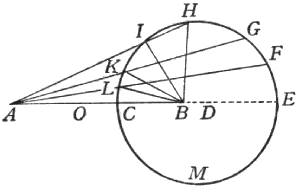
\includegraphics[width=7.50cm,height=4.80cm,keepaspectratio]{images/figura07.png} \end{center}
\end{center}

Segniamo questa linea retta \emph{AB} di qualsivoglia lunghezza; e preso in lei qualsivoglia punto \emph{C}, che in parti diseguali la divida, dico che partendosi coppie di linee da i termini \emph{A}, \emph{B}, che, ritenendo fra di loro la medesima proporzione che hanno le parti \emph{AC}, \emph{BC}, vadiano a concorrere insieme, i punti de i lor concorsi cadranno tutti nella circonferenza di un medesimo cerchio: come, per esempio, partendosi le \emph{AL}, \emph{BL} da i punti \emph{A}, \emph{B}, ed avendo tra di loro la medesima proporzione che hanno le parti \emph{AC}, \emph{BC}, ed andando a concorrere nel punto \emph{L}, e ritenendo l'istessa proporzione altre due \emph{AK}, \emph{BK}, concorrendo in \emph{K}, altre \emph{AI}, \emph{BI}, \emph{AH}, \emph{HB}, \emph{AG}, \emph{GB}, \emph{AF}, \emph{FB}, \emph{AE}, \emph{EB}, dico che i punti de i concorsi \emph{L}, \emph{K}, \emph{I}, \emph{H}, \emph{G}, \emph{F}, \emph{E} cascano tutti nella circonferenza di un istesso cerchio; talché se ci immagineremo, il punto \emph{C} muoversi continuamente con tal legge, che le linee da esso prodotte sino a i termini fissi \emph{A}, \emph{B} mantenghino sempre la proporzione medesima che hanno le prime parti \emph{AC}, \emph{CB}, tal punto \emph{C} descriverà la circonferenza d'un cerchio, come appresso vi dimostrerò; ed il cerchio in cotal modo descritto sarà sempre maggiore e maggiore infinitamente, secondo che il punto \emph{C} sarà preso più vicino al punto di mezzo, che sia \emph{O}, e minore sarà quel cerchio che dal punto più vicino all'estremità \emph{B} sarà descritto; in maniera che da i punti infiniti che pigliar si possono nella linea \emph{OB} si descriveranno cerchi (movendogli con l'esplicata legge) di qualsivoglia grandezza, minori della luce dell'occhio d'una pulce, e maggiori dell'equinoziale del primo mobile. Ora, se alzandosi qualsivoglia de i punti compresi tra i termini \emph{O}, \emph{B}, da tutti si descrivono cerchi, e immensi da i punti prossimi all'\emph{O}, alzando l'istesso \emph{O} e continuando di muoverlo con l'osservanza dell'istesso decreto, cioè che le linee da esso prodotte sino a i termini \emph{A}, \emph{B} ritenghino la proporzione che hanno le prime linee \emph{AO}, \emph{OB}, che linea verrà segnata? Segnerassi la circonferenza d'un cerchio, ma d'un cerchio maggiore di tutti gli altri massimi, di un cerchio, dunque, infinito; ma si segna anco una linea retta e perpendicolare sopra la \emph{BA}, eretta dal punto \emph{O} e prodotta in infinito senza mai tornare a riunire il suo termine ultimo col suo primo, come ben tornavano l'altre: imperò che la segnata per il moto limitato del punto \emph{C}, dopo segnato il mezzo cerchio superiore \emph{CHE}, continuava di segnare l'inferiore \emph{EMC}, riunendo insieme i suoi estremi termini nel punto \emph{C}; ma il punto \emph{O}, mossosi per segnar, come tutti gli altri della linea \emph{AB} (perché i punti presi nell'altra parte \emph{OA} descriveranno essi ancora i lor cerchi, ed i massimi i punti prossimi all'\emph{O}), il suo cerchio, per farlo massimo di tutti, e per conseguenza infinito, non può più ritornare nel suo primo termine, ed in somma descrive una linea retta infinita per circonferenza del suo infinito cerchio. Considerate ora qual differenza sia da un cerchio finito a un infinito, poiché questo muta talmente l'essere, che totalmente perde l'essere e il poter essere: ché già ben chiaramente comprendiamo, non si poter dare un cerchio infinito; il che si tira poi in consequenza, né meno poter essere una sfera infinita, né altro qualsivoglia corpo o superficie figurata e infinita. Or che diremo di cotali metamorfosi nel passar dal finito all'infinito? e perché doviamo sentir repugnanza maggiore, mentre, cercando l'infinito ne i numeri, andiamo a concluderlo nell'uno? e mentre che rompendo un solido in molte parti e seguitando di ridurlo in minutissima polvere, risoluto che si fusse ne gl'infiniti suoi atomi non più divisibili, perché non potremo dire, quello esser ritornato in un solo continuo, ma forse fluido come l'acqua o 'l mercurio o 'l medesimo metallo liquefatto? e non vediamo noi, le pietre liquefarsi in vetro, ed il vetro medesimo, co 'l molto fuoco, farsi fluido più che l'acqua?

\speaker{Sagr.} Doviamo dunque credere, i fluidi esser tali, perché sono risoluti ne i primi infiniti indivisibili, suoi componenti?

\speaker{Salv.} Io non so trovar miglior ripiego per risolver alcune sensate apparenze, tra le quali una è questa. Mentre io piglio un corpo duro, o sia pietra o metallo, e che con martello o sottilissima lima lo vo al possibile dividendo in minutissima ed impalpabile polvere, chiara cosa è che i suoi minimi, ancor che per la lor piccolezza siano impercettibili a uno a uno dalla nostra vista e dal tatto, tuttavia son eglino ancor quanti, figurati e numerabili: e di essi accade che, accumulati insieme, si sostengono ammucchiati; e scavati sino a certo segno, resta la cavità, senza che le parti d'intorno scorrano a riempirla; agitati e commossi, subito si fermano tantosto che il motore esterno gli abbandona: e questi medesimi effetti fanno ancora tutti gli aggregati di corpuscoli maggiori e maggiori, e di ogni figura, ancora che sferica, come veggiamo ne i monti di miglio, di grano, di migliarole di piombo e d'ogni altra materia. Ma se noi tenteremo di vedere tali accidenti nell'acqua, nissuno ve ne troveremo; ma, sollevata, immediatamente si spiana, se da vaso o altro esterno ritegno non sia sostenuta; incavata, subito scorre a riempire la cavità; ed agitata, per lunghissimo tempo va fluttuando, e per spazii grandissimi distendendo le sue onde. Da questo mi par di potere molto ragionevolmente arguire, i minimi dell'acqua, ne i quali ella pur sembra esser risoluta (poiché ha minor consistenza di qualsivoglia sottilissima polvere, anzi non ha consistenza nissuna), esser differentissimi da i minimi quanti e divisibili; né saprei ritrovarci altra differenza, che l'esser indivisibili. Parmi anco che la sua esquisitissima trasparenza ce ne porga assai ferma coniettura: perché se noi piglieremo del più trasparente cristallo che sia e lo cominceremo a rompere e pestare, ridotto in polvere perde la trasparenza, e sempre più quanto più sottilmente si trita; ma l'acqua, che pure è sommamente trita, è anco sommamente diafana. L'oro e l'argento, con acque forti polverizzati più sottilmente che con qualsivoglia lima, pur restano in polvere, ma non divengon fluidi, né prima si liquefanno che gl'indivisibili del fuoco o de i raggi del Sole gli dissolvano, credo ne i lor primi altissimi componenti, infiniti, indivisibili.

\speaker{Sagr.} Questo che V. S. ha toccato della luce, ho io più volte veduto con maraviglia; veduto, dico, con uno specchio concavo di tre palmi di diametro, liquefare il piombo in un instante: onde io son venuto in opinione, che quando lo specchio fusse grandissimo e ben terso e di figura parabolica, liquefarebbe non meno ogni altro metallo in brevissimo tempo, vedendo che quello, né molto grande né ben lustro e di cavità sferica, con tanta forza liquefaceva il piombo ed abbruciava ogni materia combustibile; effetti che mi rendon credibili le maraviglie de gli specchi d'Archimede.

\speaker{Salv.} Intorno a gli effetti de gli specchi d'Archimede mi rese credibile ogni miracolo, che si legge in più scrittori, la lettura de i libri dell'istesso Archimede, già da me con infinito stupore letti e studiati; e se nulla di dubbio mi fusse restato, quello che ultimamente ha dato in luce intorno allo \emph{Specchio} \emph{Ustorio} il P. Bonaventura Cavalieri, e che io con ammirazione ho letto, è bastato a cessarmi ogni difficoltà.

\speaker{Sagr.} Veddi ancor io cotesto trattato, e con gusto e maraviglia grande lo lessi; e perché per avanti avevo conoscenza della persona, mi andai confermando nel concetto che di esso avevo già preso, ch'ei fusse per riuscire uno de' principali matematici dell'età nostra. Ma tornando all'effetto maraviglioso de i raggi solari nel liquefare i metalli, doviamo noi credere che tale e sì veemente operazione sia senza moto, o pur che sia con moto, ma velocissimo?

\speaker{Salv.} Gli altri incendii e dissoluzioni veggiamo noi farsi con moto, e con moto velocissimo: veggansi le operazioni de i fulmini, della polvere nelle mine e ne i petardi, ed in somma quanto il velocitar co' i mantici la fiamma de i carboni, mista con vapori grossi e non puri, accresca di forza nel liquefare i metalli: onde io non saprei intendere che l'azzione della luce, benché purissima, potesse esser senza moto, ed anco velocissimo.

\speaker{Sagr.} Ma quale e quanta doviamo noi stimare che sia questa velocità del lume? forse instantanea, momentanea, o pur, come gli altri movimenti, temporanea? né potremo con esperienza assicurarci qual ella sia?

\speaker{Simp.} Mostra l'esperienza quotidiana, l'espansion del lume esser instantanea; mentre che vedendo in gran lontananza sparar un'artiglieria, lo splendor della fiamma senza interposizion di tempo si conduce a gli occhi nostri, ma non già il suono all'orecchie, se non dopo notabile intervallo di tempo.

\speaker{Sagr.} Eh, Sig. Simplicio, da cotesta notissima esperienza non si raccoglie altro se non che il suono si conduce al nostro udito in tempo men breve di quello che si conduca il lume; ma non mi assicura, se la venuta del lume sia per ciò istantanea, più che temporanea ma velocissima. Né simile osservazione conclude più che l'altra di chi dice: «Subito giunto il Sole all'orizonte, arriva il suo splendore a gli occhi nostri»; imperò che chi mi assicura che prima non giugnessero i suoi raggi al detto termine, che alla nostra vista?

\speaker{Salv.} La poca concludenza di queste e di altre simili osservazioni mi fece una volta pensare a qualche modo di poterci senza errore accertar, se l'illuminazione, cioè se l'espansion del lume, fusse veramente instantanea; poiché il moto assai veloce del suono ci assicura, quella della luce non poter esser se non velocissima: e l'esperienza che mi sovvenne, fu tale. Voglio che due piglino un lume per uno, il quale, tenendolo dentro lanterna o altro ricetto, possino andar coprendo e scoprendo, con l'interposizion della mano, alla vista del compagno, e che, ponendosi l'uno incontro all'altro in distanza di poche braccia, vadano addestrandosi nello scoprire ed occultare il lor lume alla vista del compagno, sì che quando l'uno vede il lume dell'altro, immediatamente scuopra il suo; la qual corrispondenza, dopo alcune risposte fattesi scambievolmente, verrà loro talmente aggiustata, che, senza sensibile svario, alla scoperta dell'uno risponderà immediatamente la scoperta dell'altro, sì che quando l'uno scuopre il suo lume, vedrà nell'istesso tempo comparire alla sua vista il lume dell'altro. Aggiustata cotal pratica in questa piccolissima distanza, pongansi i due medesimi compagni con due simili lumi in lontananza di due o tre miglia, e tornando di notte a far l'istessa esperienza, vadano osservando attentamente se le risposte delle loro scoperte ed occultazioni seguono secondo l'istesso tenore che facevano da vicino; che seguendo, si potrà assai sicuramente concludere, l'espansion del lume essere instantanea: ché quando ella ricercasse tempo, in una lontananza di tre miglia, che importano sei per l'andata d'un lume e venuta dell'altro, la dimora dovrebbe esser assai osservabile. E quando si volesse far tal osservazione in distanze maggiori, cioè di otto o dieci miglia, potremmo servirci del telescopio, aggiustandone un per uno gli osservatori al luogo dove la notte si hanno a mettere in pratica i lumi; li quali, ancor che non molto grandi, e per ciò invisibili in tanta lontananza all'occhio libero, ma ben facili a coprirsi e scoprirsi, con l'aiuto de i telescopii già aggiustati e fermati potranno esser commodamente veduti.

\speaker{Sagr.} L'esperienza mi pare d'invenzione non men sicura che ingegnosa. Ma diteci quello che nel praticarla avete concluso.

\speaker{Salv.} Veramente non l'ho sperimentata, salvo che in lontananza piccola, cioè manco d'un miglio, dal che non ho potuto assicurarmi se veramente la comparsa del lume opposto sia instantanea; ma ben, se non instantanea, velocissima, e direi momentanea, è ella, e per ora l'assimiglierei a quel moto che veggiamo farsi dallo splendore del baleno veduto tra le nugole lontane otto o dieci miglia; del qual lume distinguiamo il principio, e dirò il capo e fonte, in un luogo particolare tra esse nugole, ma bene immediatamente segue la sua espansione amplissima per le altre circostanti; che mi pare argomento, quella farsi con qualche poco di tempo; perché quando l'illuminazione fusse fatta tutta insieme, e non per parti, non par che si potesse distinguer la sua origine, e dirò il suo centro, dalle sue falde e dilatazioni estreme. Ma in quai pelaghi ci andiamo noi inavvertentemente pian piano ingolfando? tra i vacui, tra gl'infiniti, tra gli indivisibili, tra i movimenti instantanei, per non poter mai, dopo mille discorsi, giugnere a riva?

\speaker{Sagr.} Cose veramente molto sproporzionate al nostro intendimento. Ecco: l'infinito, cercato tra i numeri, par che vadia a terminar nell'unità; da gl'indivisibili nasce il sempre divisibile; il vacuo non par che risegga se non indivisibilmente mescolato tra 'l pieno: ed in somma in queste cose si muta talmente la natura delle comunemente intese da noi, che sin alla circonferenza d'un cerchio doventa una linea retta infinita; che, s'io ho ben tenuto a memoria, è quella proposizione che voi, Sig. Salviati, dovevi con geometrica dimostrazione far manifesta. Però, quando vi piaccia, sarà bene, senza più digredire, arrecarcela.

\speaker{Salv.} Eccomi a servirle, dimostrando per piena intelligenza il seguente problema:


\begin{enunciato}
Data una linea retta divisa secondo qualsivoglia proporzione in parti diseguali, descrivere un cerchio, alla cui circonferenza prodotte, a qualsivoglia punto di essa, due linee rette da i termini della data linea, ritenghino la proporzion medesima che hanno tra di loro le parti di essa linea data, sì che omologhe siano quelle che si partono da i medesimi termini.
\end{enunciato}


\begin{center}
\begin{center} 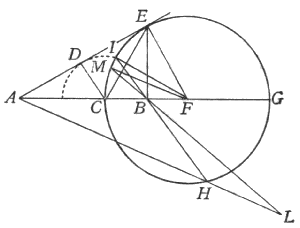
\includegraphics[width=7.50cm,height=5.70cm,keepaspectratio]{images/figura08.png} \end{center}
\end{center}

Sia la data retta linea \emph{AB}, divisa in qualsivoglia modo in parti diseguali nel punto \emph{C}: bisogna descrivere il cerchio, a qualsivoglia punto della cui circonferenza concorrendo due rette prodotte da i termini \emph{A}, \emph{B}, abbiano tra di loro la proporzion medesima che hanno tra di loro le parti \emph{AC}, \emph{BC}, sì che omologhe sian quelle che si partono dall'istesso termine. Sopra 'l centro \emph{C}, con l'intervallo della minor parte \emph{CB}, intendasi descritto un cerchio, alla circonferenza del quale venga tangente dal punto \emph{A} la retta \emph{AD}, indeterminatamente prolungata verso \emph{E}, e sia il contatto in \emph{D}, e congiungasi la \emph{CD}, che sarà perpendicolare alla \emph{AE}; ed alla \emph{BA} sia perpendicolare la \emph{BE}, la quale prodotta concorrerà con la \emph{AE}, essendo l'angolo \emph{A} acuto; sia il concorso in \emph{E}, di dove si ecciti la perpendicolare alla \emph{AE}, che prodotta vadia a concorrere con la \emph{AB}, infinitamente prolungata, in \emph{F}: dico primieramente, le due rette \emph{FE}, \emph{FC} esser eguali. Imperò che, tirata la \emph{EC}, aremo ne i due triangoli \emph{DEC}, \emph{BEC} li due lati dell'uno \emph{DE}, \emph{EC} eguali alli due dell'altro \emph{BE}, \emph{EC}, essendo le due \emph{DE}, \emph{EB} tangenti del cerchio \emph{DB}, e le basi \emph{DC}, \emph{CB} parimente eguali; onde li due angoli \emph{DEC}, \emph{BEC} saranno eguali. E perché all'angolo \emph{BCE} per esser retto manca quanto è l'angolo \emph{CEB}, ed all'angolo \emph{CEF}, pur per esser retto, manca quanto è l'angolo \emph{CED}, essendo tali mancamenti eguali, gli angoli \emph{FCE}, \emph{FEC} saranno eguali, ed in consequenza i lati \emph{FE}, \emph{FC}; onde fatto centro il punto \emph{F}, e con l'intervallo \emph{FE} descrivendo un cerchio, passerà per il punto \emph{C}. Descrivasi, e sia \emph{CEG}: dico, questo esser il cerchio ricercato, a qualsivoglia punto della circonferenza del quale ogni coppia di linee che vi concorrano, partendosi da i termini \emph{A}, \emph{B}, aranno la medesima proporzione tra di loro che hanno le due parti \emph{AC}, \emph{BC}, le quali di già vi concorrono nel punto \emph{C}. Questo, delle due che concorrono nel punto \emph{E}, cioè delle \emph{AE}, \emph{BE}, è manifesto, essendo l'angolo \emph{E} del triangolo \emph{AEB} diviso in mezzo dalla \emph{CE}; per lo che qual proporzione ha la \emph{AC} alla \emph{CB}, tale ha la \emph{AE} alla \emph{BE}. L'istesso proveremo delle due \emph{AG}, \emph{BG}, terminate nel punto \emph{G}. Imperò che, essendo (per la similitudine de' triangoli \emph{AFE}, \emph{EFB}) come \emph{AF} ad \emph{FE} così \emph{EF} ad \emph{FB}, cioè come \emph{AF} ad \emph{FC} così \emph{CF} ad \emph{FB}, sarà, dividendo, come \emph{AC} a \emph{CF} (cioè ad \emph{FG}) così \emph{CB} a \emph{FB}, e tutta \emph{AB} a tutta \emph{BG} come una \emph{CB} ad una \emph{BF}, e, componendo, come \emph{AG} a \emph{GB} così \emph{CF} ad \emph{FB}, cioè \emph{FE} ad \emph{FB}, cioè \emph{AE} ad \emph{EB}, ed \emph{AC} a \emph{CB}: il che bisognava provare. Prendasi ora qualsivoglia altro punto nella circonferenza, e sia \emph{H}, al quale concorrano le due \emph{AH}, \emph{BH}: dico parimente, come \emph{AC} a \emph{CB}, così essere \emph{AH} ad \emph{HB}. Prolunghisi \emph{HB} sino alla circonferenza in \emph{I}, e congiungasi \emph{IF}: e perché già si è visto, come \emph{AB} a \emph{BG}, così essere \emph{CB} a \emph{BF}, sarà il rettangolo \emph{ABF} eguale al rettangolo \emph{CBG}, cioè \emph{IBH}, e però come \emph{AB} a \emph{BH}, così \emph{IB} a \emph{BF}; e sono gli angoli al \emph{B} eguali; adunque \emph{AH} ad \emph{HB} sta come \emph{IF}, cioè \emph{EF}, ad \emph{FB}, ed \emph{AE} ad \emph{EB}.

Dico, oltre a ciò, che è impossibile che le linee che abbiano tal proporzione, partendosi da i termini \emph{A}, \emph{B}, concorrano a verun punto o dentro o fuori del cerchio \emph{CEG}. Imperò che, se è possibile, concorrano due tali linee al punto \emph{L}, posto fuori, e siano le \emph{AL}, \emph{BL}, e prolunghisi la \emph{LB} sino alla circonferenza in \emph{M}, e congiungasi \emph{MF}. Se dunque la \emph{AL} alla \emph{BL} è come la \emph{AC} alla \emph{BC}, cioè come la \emph{MF} alla \emph{FB}, aremo due triangoli \emph{ALB}, \emph{MFB}, li quali intorno alli due angoli \emph{ALB}, \emph{MFB} hanno i lati proporzionali, gli angoli alla cima nel punto \emph{B} eguali, e li due rimanenti \emph{FMB}, \emph{LAB} minori che retti (imperò che l'angolo retto al punto \emph{M} ha per base tutto il diametro \emph{CG}, e non la sola parte \emph{BF}; e l'altro al punto \emph{A} è acuto, perché la linea \emph{AL}, omologa della \emph{AC}, è maggiore della \emph{BL}, omologa della \emph{BC}); adunque i triangoli \emph{ABL}, \emph{MBF} son simili, e però come \emph{AB} a \emph{BL} così \emph{MB} a \emph{BF}, onde il rettangolo \emph{ABF} sarà eguale al rettangolo \emph{MBL}: ma il rettangolo \emph{ABF} s'è dimostrato eguale al \emph{CBG}: adunque il rettangolo \emph{MBL} è eguale al rettangolo \emph{CBG}, il che è impossibile: adunque il concorso non può cader fuor del cerchio. E nel medesimo modo si dimostrerà, non poter cader dentro: adunque tutti i concorsi cascano nella circonferenza stessa.

Ma è tempo che torniamo a dar sodisfazione al desiderio del Sig. Simplicio, mostrandogli come il risolver la linea ne' suoi infiniti punti non è non solamente impossibile, ma né meno ha in sé maggior difficoltà che 'l distinguere le sue parti quante, fatto però un supposto, il quale penso, Sig. Simplicio, che non siate per negarmi: e questo è, che non mi ricercherete che io vi separi i punti l'uno dall'altro e ve li faccia veder a uno a uno distinti sopra questa carta, perché io ancora mi contenterei che, senza staccar l'una dall'altra le quattro o le sei parti d'una linea, mi mostraste le sue divisioni segnate, o al più piegate ad angoli, formandone un quadrato o un essagono; perché mi persuado pure che allora le chiamereste a bastanza distinte ed attuate.

\speaker{Simp.} Veramente sì.

\speaker{Salv.} Ora, se l'inflettere una linea ad angoli, formandone ora un quadrato, ora un ottangolo, ora un poligono di quaranta, di cento o mille angoli, è mutazione bastante a ridurre all'atto quelle quattro, otto, quaranta, cento e mille parti che prima nella linea diritta erano, per vostro detto, in potenza, quando io formi di lei un poligono di lati infiniti, cioè quando io la infletta nella circonferenza d'un cerchio, non potrò io con pari licenza dire d'aver ridotto all'atto quelle parti infinite, che voi prima, mentre era retta, dicevi esser in lei contenute in potenza? Né si può negare, tal risoluzione esser fatta ne' suoi infiniti punti non meno che quella delle sue quattro parti nel formarne un quadrato, o nelle sue mille nel formarne un millagono; imperò che in lei non manca veruna delle condizioni che si trovano nel poligono di mille e di cento mila lati. Questo, applicato a una linea retta, se gli posa sopra toccandola con uno de' suoi lati, cioè con una sua centomillesima parte; il cerchio, che è un poligono di lati infiniti, tocca la medesima retta con uno de' suoi lati, che è un sol punto, diverso da tutti i suoi collaterali, e perciò da quelli diviso e distinto non meno che un lato del poligono da i suoi conterminali: e come il poligono rivoltato sopra un piano stampa con i toccamenti conseguenti de' suoi lati una linea retta eguale al suo perimetro, così il cerchio girato sopra un tal piano descrive con gl'infiniti suoi successivi contatti una linea retta egual alla propria circonferenza. Non so adesso, Sig. Simplicio, se i Signori Peripatetici, a i quali io ammetto, come verissimo concetto, il continuo esser divisibile in sempre divisibili, sì che continuando una tal divisione e suddivisione mai non si perverrebbe alla fine, si contenteranno di concedere a me, niuna delle tali loro divisioni esser l'ultima, come veramente non è, poiché sempre ve ne resta un'altra, ma bene l'ultima ed altissima esser quella che lo risolve in infiniti indivisibili, alla quale concedo che non si perverrebbe mai dividendo successivamente in maggiore e maggior moltitudine di parti; ma servendosi della maniera che propongo io, di distinguere e risolvere tutta la infinità in un tratto solo (artifizio che non mi dovrebbe esser negato), crederei che dovessero quietarsi, ed ammetter questa composizione del continuo di atomi assolutamente indivisibili, e massime essendo questa una strada forse più d'ogni altra corrente per trarci fuori di molto intrigati laberinti, quali sono, oltre a quello già toccato dalla coerenza delle parti de i solidi, il comprender come stia il negozio della rarefazzione e della condensazione, senza incorrer per causa di quella nell'inconveniente di dovere ammettere spazii vacui, e per questa la penetrazione de i corpi: inconvenienti, che amendue mi pare ch'assai destramente vengano schivati con l'ammetter detta composizione d'indivisibili.

\speaker{Simp.} Io non so quello che i Peripatetici fusser per dire, atteso che le considerazioni fatte da voi credo che gli giugnerebbero per la maggior parte nuove, e come tali converrebbe esaminarle; e potrebbe accadere che quelli vi ritrovassero risposte e soluzioni potenti a sciorre quei nodi, che io, per la brevità del tempo e per la debolezza del mio ingegno, non saprei di presente risolvere. Però sospendendo per ora questa parte, sentirei ben volentieri come l'introduzzione di questi indivisibili faciliti l'intelligenza della condensazione e della rarefazzione, schivando nell'istesso tempo il vacuo e la penetrazion de i corpi.

\speaker{Sagr.} Sentirò io ancora con gran brama la medesima cosa, all'intelletto mio tanto oscura; con questo però, che io non rimanga defraudato di sentire, conforme a quello che poco fa disse il Sig. Simplicio, le ragioni d'Aristotele in confutazion del vacuo, ed in consequenza le soluzioni che voi gli arrecate, come convien fare mentre voi ammettete quello che esso nega.

\speaker{Salv.} Faremo l'uno e l'altro. E quanto al primo, è necessario che, sì come in grazia della rarefazzione ci serviamo della linea descritta dal minor cerchio, maggiore della propria circonferenza, mentre vien mosso alla revoluzione del maggiore, così per intelligenza della condensazione mostriamo come alla conversione fatta dal minor cerchio il maggiore descriva una linea retta minore della sua circonferenza; per la cui più chiara esplicazione, porremo innanzi la considerazione di quello che accade ne i poligoni.


\begin{center}
\begin{center} 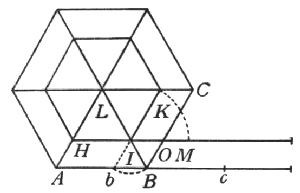
\includegraphics[width=7.50cm,height=4.83cm,keepaspectratio]{images/figura09.png} \end{center}
\end{center}

In una descrizzione simile a quell'altra, siano due essagoni circa il comune centro \emph{L}, che siano questi \emph{ABC}, \emph{HIK}, con le linee parallele \emph{HOM}, \emph{ABc}, sopra le quali si abbiano a far le revoluzioni; e fermato l'angolo \emph{I} del poligono minore, volgasi esso poligono sin che il lato \emph{IK} caschi sopra la parallela, nel qual moto il punto \emph{K} descriverà l'arco \emph{KM}, e 'l lato \emph{KI} si unirà con la parte \emph{IM}: tra tanto bisogna vedere quel che farà il lato \emph{CB} del poligono maggiore. E perché il rivolgimento si fa sopra il punto \emph{I}, la linea \emph{IB} col termine suo \emph{B} descriverà, tornando indietro, l'arco \emph{Bb} sotto alla parallela \emph{cA}, tal che quando il lato \emph{KI} si congiugnerà con la linea \emph{MI}, il lato \emph{BC} si unirà con la linea \emph{bc}, con l'avanzarsi per l'innanzi solamente quanto è la parte \emph{Bc} e ritirando in dietro la parte suttesa all'arco \emph{Bb}, la quale vien sopraposta alla linea \emph{BA}. Ed intendendo continuarsi nell'istesso modo la conversione fatta dal minor poligono, questo descriverà bene e passerà sopra la sua parallela una linea eguale al suo perimetro; ma il maggiore passerà una linea minore del suo perimetro la quantità di tante linee \emph{bB} quanti sono uno manco de' suoi lati; e sarà tal linea prossimamente eguale alla descritta dal poligono minore, eccedendola solamente di quanto è la \emph{bB}. Qui dunque senza veruna repugnanza si scorge la cagione per la quale il maggior poligono non trapassi (portato dal minore) con i suoi lati linea maggiore della passata dal minore; che è perché una parte di ciascheduno de' lati si soprappone al suo precedente conterminale.


\begin{center}
\begin{center} 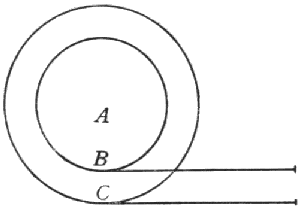
\includegraphics[width=7.50cm,height=5.25cm,keepaspectratio]{images/figura10.png} \end{center}
\end{center}

Ma se considereremo i due cerchi intorno al centro \emph{A}, li quali sopra le lor parallele posino, toccando il minore la sua nel punto \emph{B}, ed il maggiore la sua nel punto \emph{C}, qui nel cominciar a far la revoluzione del minore non avverrà che il punto \emph{B} resti per qualche tempo immobile, sì che la linea \emph{BC} dando in dietro trasporti il punto \emph{C}, come accadeva ne i poligoni, che restando fisso il punto \emph{I} sin che il lato \emph{KI} cadesse sopra la linea \emph{IM}, la linea \emph{IB} riportava in dietro il \emph{B}, termine del lato \emph{CB}, sino in \emph{b}, onde il lato \emph{BC} cadeva in \emph{bc}, soprapponendo alla linea \emph{BA} la parte \emph{Bb} e solo avanzandosi per l'innanzi la parte \emph{Bc}, eguale alla \emph{IM}, cioè a un lato del poligono minore; per le quali soprapposizioni, che sono gli eccessi de i lati maggiori sopra i minori, gli avanzi che restano, eguali a i lati del minor poligono, vengono a comporre nell'intera revoluzione la linea retta eguale alla segnata e misurata dal poligono minore. Ma qui dico, che se noi vorremo applicare un simil discorso all'effetto de i cerchi, converrà dire, che dove i lati di qualsivoglia poligono son compresi da qualche numero, i lati del cerchio sono infiniti: quelli son quanti e divisibili; questi, non quanti e indivisibili: i termini de i lati del poligono nella revoluzione stanno per qualche tempo fermi, cioè ciascheduno tal parte del tempo di una intera conversione, qual parte esso è di tutto il perimetro; ne i cerchi similmente le dimore de' termini de' suoi infiniti lati son momentanee, perché tal parte è un instante d'un tempo quanto, qual è un punto d'una linea, che ne contiene infiniti: i regressi in dietro fatti da i lati del maggior poligono sono non di tutto 'l lato, ma solamente dell'eccesso suo sopra 'l lato del minore, acquistando per l'innanzi tanto di spazio quanto è il detto minor lato; ne i cerchi il punto o lato C, nella quiete instantanea del termine \emph{B}, si ritira in dietro quanto è il suo eccesso sopra 'l lato \emph{B}, acquistando per l'innanzi quanto è il medesimo \emph{B}: ed in somma gl'infiniti lati indivisibili del maggior cerchio con gl'infiniti indivisibili ritiramenti loro, fatti nell'infinite instantanee dimore de gl'infiniti termini de gl'infiniti lati del minor cerchio, e con i loro infiniti progressi, eguali a gl'infiniti lati di esso minor cerchio, compongono e disegnano una linea eguale alla descritta dal minor cerchio, contenente in sé infinite soprapposizioni non quante, che fanno una costipazione e condensazione senza veruna penetrazione di parti quante, quale non si può intendere farsi nella linea divisa in parti quante, quale è il perimetro di qualsivoglia poligono, il quale, disteso in linea retta, non si può ridurre in minor lunghezza se non col far che i lati si soprapponghino e penetrino l'un l'altro. Questa costipazione di parti non quante ma infinite, senza penetrazione di parti quante, e la prima distrazzione di sopra dichiarata de gl'infiniti indivisibili con l'interposizione di vacui indivisibili, credo che sia il più che dir si possa per la condensazione e rarefazzione de i corpi, senza necessità d'introdurre la penetrazione de i corpi e gli spazii quanti vacui. Se ci è cosa che vi gusti, fatene capitale; se no, reputatela vana, e 'l mio discorso ancora, e ricercate da qualche altro esplicazione di maggior quiete per l'intelletto. Solo queste due parole vi replico, che noi siamo tra gl'infiniti e gl'indivisibili.

\speaker{Sagr.} Che il pensiero sia sottile, ed a' miei orecchi nuovo e peregrino, lo confesso liberamente; se poi nel fatto stesso la natura proceda con tal ordine, non saprei che risolvermi: vero è che sin ch'io non sentissi cosa che maggiormente mi quietassi, per non rimaner muto affatto, m'atterrei a questa. Ma forse il Sig. Simplicio avrà (quello che sin qui non ho incontrato) modo di esplicare l'esplicazione che in materia così astrusa da i filosofi si arreca; ché in vero quel che sin qui ho letto circa la condensazione è per me così denso, e quel della rarefazzione così sottile, che la mia debol vista questo non comprende e quello non penetra.

\speaker{Simp.} Io son pieno di confusione, e trovo duri intoppi nell'un sentiero e nell'altro, ed in particolare in questo nuovo: perché, secondo questa regola, un'oncia d'oro si potrebbe rarefare e distrarre in una mole maggiore di tutta la Terra, e tutta la Terra condensare e ridurre in minor mole di una noce, cose che io non credo, né credo che voi medesimo crediate; e le considerazioni e dimostrazioni sin qui fatte da voi, come che son cose matematiche, astratte e separate dalla materia sensibile, credo che applicate alle materie fisiche e naturali non camminerebbero secondo coteste regole.

\speaker{Salv.} Che io vi sia per far vedere l'invisibile, né io lo saprei fare, né credo voi lo ricerchiate; ma per quanto da i nostri sensi può esser compreso, già che voi avete nominato l'oro, non veggiam noi farsi immensa distrazzione delle sue parti? Non so se vi sia occorso di veder le maniere che tengono gli artefici in condur l'oro tirato, il quale non è veramente oro se non in superficie, ma la materia interna è argento: ed il modo del condurlo è tale. Pigliano un cilindro, o volete dire una verga, d'argento, lunga circa mezzo braccio e grossa per tre o quattro volte il dito pollice, e questa indorano con foglie d'oro battuto, che sapete esser così sottile che quasi va vagando per l'aria, e di tali foglie ne soprappongono otto o dieci, e non più. Dorato che è, cominciano a tirarlo con forza immensa, facendolo passare per fori della filiera; e tornando a farlo ripassare molte e molte volte successivamente per fori più angusti, dopo molte e molte ripassate lo riducono alla sottigliezza d'un capello di donna, se non maggiore: e tuttavia resta dorato in superficie. Lascio ora considerare a voi quale sia la sottigliezza e distrazzione alla quale si è ridotta la sustanza dell'oro.

\speaker{Simp.} Io non veggo che da questa operazione venga in consequenza un assottigliamento della materia dell'oro da farne quelle maraviglie che voi vorreste: prima, perché già la prima doratura fu di dieci foglie d'oro, che vengono a far notabile grossezza; secondariamente, se ben, nel tirare e assottigliar quell'argento, cresce in lunghezza, scema però anco tanto in grossezza, che, compensando l'una dimensione con l'altra, la superficie non si agumenta tanto, che per vestir l'argento di oro, bisogni ridurlo a sottigliezza maggiore di quella delle prime foglie.

\speaker{Salv.} V'ingannate d'assai, Sig. Simplicio, perché l'accrescimento della superficie è sudduplo dell'allungamento, come io potrei geometricamente dimostrarvi.

\speaker{Sagr.} Io, e per me e per il Sig. Simplicio, vi pregherei a recarci tal dimostrazione, se però credete che da noi possa esser capita.

\speaker{Salv.} Vedrò se così improvisamente mi torna a memona. Già è manifesto, che quel primo grosso cilindro d'argento ed il filo lunghissimo tirato sono due cilindri eguali, essendo l'istesso argento; tal che s'io mostrerò qual proporzione abbiano tra di loro le superficie de i cilindri eguali, averemo l'intento. Dico per tanto che:


\begin{enunciato}
Le superficie de i cilindri eguali, trattone le basi, son tra di loro in sudduplicata proporzione delle loro lunghezze.
\end{enunciato}


\begin{center}
\begin{center} 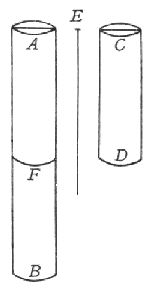
\includegraphics[width=3.75cm,height=7.18cm,keepaspectratio]{images/figura11.png} \end{center}
\end{center}

Siano due cilindri eguali, l'altezze de i quali \emph{AB}, \emph{CD}, e sia la linea \emph{E} media proporzionale tra esse: dico, la superficie del cilindro \emph{AB}, trattone le basi, alla superficie del cilindro \emph{CD}, trattone parimente le basi, aver la medesima proporzione che la linea \emph{AB} alla linea \emph{E}, che è suddupla dalla proporzione di \emph{AB} a \emph{CD}. Taglisi la parte del cilindro \emph{AB} in \emph{F}, e sia l'altezza \emph{AF} eguale alla \emph{CD}: e perché le basi de' cilindri eguali rispondon contrariamente alle loro altezze, il cerchio base del cilindro \emph{CD} al cerchio base del cilindro \emph{AB} sarà come l'altezza \emph{BA} alla \emph{DC}; e perché i cerchi son tra loro come i quadrati de i diametri, aranno detti quadrati la medesima proporzione che la \emph{BA} alla \emph{CD}; ma come \emph{BA} a \emph{CD}, così il quadrato \emph{BA} al quadrato della \emph{E}: son dunque tali quattro quadrati proporzionali; e però i lor lati ancora saranno proporzionali, e come la linea \emph{AB} alla \emph{E}, così il diametro del cerchio \emph{C} al diametro del cerchio \emph{A}. Ma come i diametri, così sono le circonferenze, e come le circonferenze così sono ancora le superficie de' cilindri egualmente alti: adunque come la linea \emph{AB} alla \emph{E}, così la superficie del cilindro \emph{CD} alla superficie del cilindro \emph{AF}. Perché dunque l'altezza \emph{AF} alla \emph{AB} sta come la superficie \emph{AF} alla superficie \emph{AB}; e come l'altezza \emph{AB} alla linea \emph{E}, così la superficie \emph{CD} alla \emph{AF}: sarà, per la perturbata, come l'altezza \emph{AF} alla \emph{E}, così la superficie \emph{CD} alla superficie \emph{AB}: e convertendo, come la superficie del cilindro \emph{AB} alla superficie del cilindro \emph{CD}, così la linea \emph{E} alla \emph{AF}, cioè alla \emph{CD}, o vero la \emph{AB} alla \emph{E}, che è proporzione suddupla della \emph{AB} alla \emph{CD}: che è quello che bisognava provare.

Ora, se noi applicheremo questo, che si è dimostrato, al nostro proposito, presupposto che quel cilindro d'argento, che fu dorato mentre non era più lungo di mezzo braccio e grosso tre o quattro volte più del dito pollice, assottigliato alla finezza d'un capello si sia allungato sino in venti mila braccia (che sarebbe anche più assai), troveremo, la sua superficie esser cresciuta dugento volte più di quello che era; ed in consequenza quelle foglie d'oro, che furon soprapposte dieci in numero, distese in superficie dugento volte maggiore, ci assicurano, l'oro, che cuopre la superficie delle tante braccia di filo, restar non più grosso che la ventesima parte d'una foglia dell'ordinario oro battuto. Considerate ora voi qual sia la sua sottigliezza, e se è possibile concepirla fatta senza una immensa distrazzione di parti, e se questa vi pare una esperienza che tenda anche ad una composizione d'infiniti indivisibili nelle materie fisiche: se ben di ciò non mancano altri più gagliardi e concludenti rincontri.

\speaker{Sagr.} La dimostrazione mi par tanto bella, che quando non avesse forza di persuader quel primo intento per il quale è stata prodotta (che pur mi par che ve l'abbia grande), ad ogni modo benissimo si è impiegato questo breve tempo che per sentirla si è speso.

\speaker{Salv.} Già che veggo che gustate tanto di queste geometriche dimostrazioni, apportatrici di guadagni sicuri, vi dirò la compagna di questa, che sodisfà ad un quesito curioso assai. Nella passata aviamo quello che accaggia de i cilindri eguali, ma diversi di altezze o vero lunghezze: è ben sentire quello che avvenga a i cilindri eguali di superficie, ma diseguali d'altezze; intendendo sempre delle superficie sole che gli circondano intorno, cioè non comprendendo le due basi, superiore e inferiore. Dico dunque che:


\begin{enunciato}
I cilindri retti, le superfici de i quali, trattone le basi, siano eguali, hanno fra di loro la medesima proporzione che le loro altezze contrariamente prese.
\end{enunciato}


\begin{center}
\begin{center} 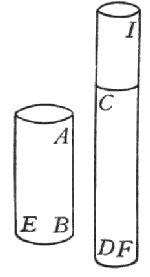
\includegraphics[width=3.75cm,height=6.93cm,keepaspectratio]{images/figura12.png} \end{center}
\end{center}

Siano eguali le superficie de i due cilindri \emph{AE}, \emph{CF}, ma l'altezza di questo \emph{CD} maggiore dell'altezza dell'altro \emph{AB}: dico, il cilindro \emph{AE} al cilindro \emph{CF} aver la medesima proporzione che l'altezza \emph{CD} alla \emph{AB}. Perché dunque la superficie \emph{CF} è uguale alla superficie \emph{AE}, sarà il cilindro \emph{CF} minore dell'\emph{AE}, perché se li fusse eguale, la sua superficie, per la passata proposizione, sarebbe maggiore della superficie \emph{AE}, e molto più se il medesimo cilindro \emph{CF} fusse maggiore dell'\emph{AE}. Intendasi il cilindro \emph{ID} eguale all'\emph{AE}; adunque, per la precedente, la superficie del cilindro \emph{ID} alla superficie dell'\emph{AE} starà come l'altezza \emph{IF} alla media tra \emph{IF}, \emph{AB}. Ma essendo, per il dato, la superficie \emph{AE} eguale alla \emph{CF}, ed avendo la superficie \emph{ID} alla \emph{CF} la medesima proporzione che l'altezza \emph{IF} alla \emph{CD}, adunque la \emph{CD} è media tra le \emph{IF}, \emph{AB}; in oltre, essendo il cilindro \emph{ID} eguale al cilindro \emph{AE}, aranno amendue la medesima proporzione al cilindro \emph{CF}: ma l'\emph{ID} al \emph{CF} sta come l'altezza \emph{IF} alla \emph{CD}: adunque il cilindro \emph{AE} al cilindro \emph{CF} arà la medesima proporzione che la linea \emph{IF} alla \emph{CD}, cioè che la \emph{CD} alla \emph{AB}, che è l'intento.

Di qui s'intende la ragione d'un accidente che non senza maraviglia vien sentito dal popolo; ed è, come possa essere che il medesimo pezzo di tela più lungo per un verso che per l'altro, se se ne facesse un sacco da tenervi dentro del grano, come si costuma fare con un fondo di tavola, terrà più servendoci per l'altezza del sacco della minor misura della tela e con l'altra circondando la tavola del fondo, che facendo per l'opposito: come se, v. g., la tela per un verso fusse sei braccia e per l'altro dodici, più terrà quando con la lunghezza di dodici si circondi la tavola del fondo, restando il sacco alto braccia sei, che se si circondasse un fondo di sei braccia, avendone dodici per altezza. Ora, da quello che si è dimostrato, alla generica notizia del capir più per quel verso che per questo, si aggiugne la specifica e particolare scienza del quanto ei contenga più; che è, che tanto più terrà quanto sarà più basso, e tanto meno quanto più alto: e così, nelle misure assegnate essendo la tela il doppio più lunga che larga, cucita per la lunghezza terrà la metà manco che per l'altro verso; e parimente avendo una stuoia, per fare una bugnola, lunga venticinque braccia e larga, v. g., sette, piegata per lo lungo terrà solamente sette misure di quelle che per l'altro verso ne terrebbe venticinque.

\speaker{Sagr.} E così con nostro gusto particolare andiamo continuamente acquistando nuove cognizioni curiose e non ignude di utilità. Ma nel proposito toccato adesso, veramente non credo che tra quelli che mancano di qualche cognizione di geometria se ne trovassero quattro per cento che non restassero a prima giunta ingannati, che quei corpi che da superficie eguali son contenuti, non fussero ancora in tutto eguali; sì come nell'istesso errore incorrono parlando delle superficie, che per determinar, come spesse volte accade, delle grandezze di diverse città, intera cognizione gli par d'averne qualunque volta sanno la quantità de i recinti di quelle, ignorando che può essere un recinto eguale a un altro, e la piazza contenuta da questo assai maggiore della piazza di quello: il che accade non solamente tra le superficie irregolari, ma tra le regolari, delle quali quelle di più lati son sempre più capaci di quelle di manco lati, sì che in ultimo il cerchio, come poligono di lati infiniti, è capacissimo sopra tutti gli altri poligoni di egual circuito; di che mi ricordo averne con gusto particolare veduta la dimostrazione studiando la Sfera del Sacrobosco con un dottissimo commentario sopra.

\speaker{Salv.} È verissimo: ed avendo io ancora incontrato cotesto luogo, mi dette occasione di ritrovare, come con una sola e breve dimostrazione si concluda, il cerchio esser maggiore di tutte le figure regolari isoperimetre; e, dell'altre, quelle di più lati, maggiori di quelle di manco.

\speaker{Sagr.} Ed io, che sento tanto diletto in certe proposizioni e dimostrazioni scelte e non triviali, importunandovi vi prego che me ne facciate partecipe.

\speaker{Salv.} In brevi parole vi spedisco, dimostrando il seguente teorema, cioè:


\begin{enunciato}
Il cerchio è medio proporzionale tra qualsivoglino due poligoni regolari tra di loro simili, de i quali uno gli sia circoscritto e l'altro gli sia isoperimetra. In oltre, essendo egli minore di tutti i circoscritti, all'incontro massimo di tutti gl'isoperimetri. De i medesimi poi circoscritti, quelli che hanno più angoli son minori di quelli che ne hanno manco; ma all'incontro, de gl'isoperimetri quelli di più angoli son maggiori.
\end{enunciato}


\begin{center}
\begin{center} 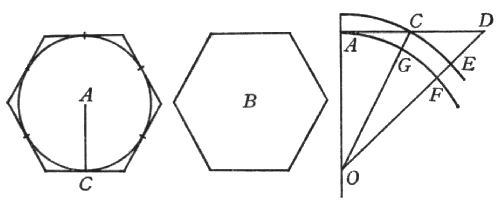
\includegraphics[width=11.20cm,height=5.03cm,keepaspectratio]{images/figura13.png} \end{center}
\end{center}

Delli due poligoni simili \emph{A}, \emph{B} sia l'\emph{A} circoscritto al cerchio \emph{A}, e l'altro \emph{B} ad esso cerchio sia isoperimetro: dico, il cerchio esser medio proporzionale tra essi. Imperò che (tirato il semidiametro \emph{AC}), essendo il cerchio eguale a quel triangolo rettangolo, de i lati del quale che sono intorno all'angolo retto, uno sia eguale al semidiametro \emph{AC} e l'altro alla circonferenza; e similmente essendo il poligono \emph{A} eguale al triangolo rettangolo, che intorno all'angolo retto ha uno de i lati eguali alla medesima retta \emph{AC}, e l'altro al perimetro del medesimo poligono; è manifesto, il circoscritto poligono aver al cerchio la medesima proporzione che ha il suo perimetro alla circonferenza di esso cerchio, cioè al perimetro del poligono \emph{B}, che alla circonferenza detta si pone eguale: ma il poligono \emph{A} al \emph{B} ha doppia proporzione che 'l suo perimetro al perimetro di \emph{B} (essendo figure simili): adunque il cerchio \emph{A} è medio proporzionale tra i due poligoni \emph{A}, \emph{B}. Ed essendo il poligono \emph{A} maggior del cerchio \emph{A}, è manifesto, esso cerchio \emph{A} esser maggiore del poligono \emph{B} suo isoperimetro, ed in consequenza massimo di tutti i poligoni regolari suoi isoperimetri.

Quanto all'altra parte, cioè di provare che de i poligoni circoscritti al medesimo cerchio, quello di manco lati sia maggior di quello di più lati; ma che all'incontro, de i poligoni isoperimetri quello di più lati sia maggiore di quello di manco lati; dimostreremo così. Nel cerchio, il cui centro \emph{O}, semidiametro \emph{OA}, sia la tangente \emph{AD}, ed in essa pongasi, per esempio, \emph{AD} esser la metà del lato del pentagono circoscritto, ed \emph{AC} metà del lato dell'ettagono, e tirinsi le rette \emph{OGC}, \emph{OFD}, e, centro \emph{O}, intervallo \emph{OC}, descrivasi l'arco \emph{ECI}. E perché il triangolo \emph{DOC} è maggiore del settore \emph{EOC}, e 'l settore \emph{COI} maggiore del triangolo \emph{COA}, maggior proporzione arà il triangolo \emph{DOC} al triangolo \emph{COA}, che 'l settore \emph{EOC} al settore \emph{COI}, cioè che 'l settore \emph{FOG} al settore \emph{GOA}; e componendo e permutando, il triangolo \emph{DOA} al settore \emph{FOA} arà maggior proporzione che il triangolo \emph{COA} al settore \emph{GOA}, e dieci triangoli \emph{DOA} a dieci settori \emph{FOA} aranno maggior proporzione che quattordici triangoli \emph{COA} a quattordici settori \emph{GOA}, cioè il pentagono circoscritto arà maggior proporzione al cerchio che non gli ha l'ettagono; e però il pentagono sarà maggior dall'ottagono. Intendansi ora un ettagono ed un pentagono isoperimetri al medesimo cerchio: dico, l'ettagono esser maggior del pentagono. Imperò che, essendo l'istesso cerchio medio proporzionale tra 'l pentagono circoscritto e 'l pentagono suo isoperimetro, e parimente medio tra 'l circoscritto e l'isoperimetro ettagono; essendosi provato, il circoscritto pentagono esser maggiore del circoscritto ettagono; avrà esso pentagono maggior proporzione al cerchio che l'ettagono, cioè il cerchio arà maggior proporzione al suo isoperimetro pentagono che all'isoperimetro ettagono: adunque il pentagono è minore dell'isoperimetro ettagono: che si doveva dimostrare.

\speaker{Sagr.} Gentilissima dimostrazione e molto acuta. Ma dove siamo trascorsi a ingolfarci nella geometria? mentre eramo su 'l considerare le difficoltà promosse dal Sig. Simplicio, che veramente son di gran considerazione; ed in particolare quella della condensazione mi par durissima.

\speaker{Salv.} Se la condensazione e la rarefazzione son moti opposti, dove si vegga una immensa rarefazzione, non si potrà negare una non men grandissima condensazione; ma rarefazzioni immense, e, quel che accresce la maraviglia, quasi che momentanee, le veggiamo noi tutto 'l giorno. E quale sterminata rarefazzione è quella di una poca quantità di polvere d'artiglieria, risoluta in una mole vastissima di fuoco? e quale, oltre a questa, l'espansione, direi quasi senza termine, della sua luce? E se quel fuoco e questo lume si riunissero insieme, che pur non è impossibile, poiché dianzi stettero dentro quel piccolo spazio, qual condensamento sarebbe questo? Voi, discorrendo, troverete mille di tali rarefazzioni, che sono molto più in pronto ad esser osservate che le condensazioni, perché le materie dense son più trattabili e sottoposte a i nostri sensi, che ben maneggiamo le legne e le vediamo risolvere in fuoco e in luce, ma non così veggiamo il fuoco e 'l lume condensarsi a costituire il legno; veggiamo i frutti, i fiori e mille altre solide materie risolversi in gran parte in odori, ma non così osserviamo gli atomi odorosi concorrere alla costituzione de i solidi odorati. Ma dove manca la sensata osservazione, si deve supplir col discorso, che basterà per farci capaci non men del moto alla rarefazzione e resoluzione de i solidi, che alla condensazione delle sustanze tenui e rarissime. In oltre, noi trattiamo come si possa far la condensazione e rarefazzione de i corpi che si possono rarefare e condensare, specolando in qual maniera ciò possa esser fatto senza l'introduzzion del vacuo e della penetrazione de i corpi; il che non esclude che in natura possano esser materie che non ammettono tali accidenti, ed in consequenza non danno luogo a quelli che voi chiamate inconvenienti e impossibili. E finalmente. Sig. Simplicio, io, in grazia di voi altri, Signori filosofi, mi sono affaticato in specolare come si possa intendere, farsi la condensazione e la rarefazzione senza ammetter la penetrazione de i corpi e l'introduzzione de gli spazii vacui, effetti da voi negati ed aborriti; che quando voi gli voleste concedere, io non vi sarei così duro contradittore. Però, o ammettete questi inconvenienti, o gradite le mie specolazioni, o trovatene di più aggiustate.

\speaker{Sagr.} Alla negativa della penetrazione son io del tutto con i filosofi peripatetici. A quella del vacuo vorrei sentir ben ponderare la dimostrazione d'Aristotele, con la quale ei l'impugna, e quello che voi, Sig. Salviati, gli opponete. Il Sig. Simplicio mi farà grazia di arrecar puntualmente la prova del Filosofo, e voi Sig. Salviati, la risposta.

\speaker{Simp.} Aristotele, per quanto mi sovviene, insurge contro alcuni antichi, i quali introducevano il vacuo come necessario per il moto, dicendo che questo senza quello non si potrebbe fare. A questo contrapponendosi Aristotele, dimostra che, all'opposito, il farsi (come veggiamo) il moto distrugge la posizione del vacuo; e 'l suo progresso è tale. Fa due supposizioni: l'una è di mobili diversi in gravità, mossi nel medesimo mezzo; l'altra è dell'istesso mobile mosso in diversi mezzi. Quanto al primo, suppone che mobili diversi in gravità si muovano nell'istesso mezzo con diseguali velocità, le quali mantengano tra di loro la medesima proporzione che le gravità; sì che, per esempio, un mobile dieci volte più grave di un altro si muova dieci volte più velocemente. Nell'altra posizione piglia che le velocità del medesimo mobile in diversi mezzi ritengano tra di loro la proporzione contraria di quella che hanno le grossezze o densità di essi mezzi; talmente che, posto, v. g., che la crassizie dell'acqua fusse dieci volte maggiore di quella dell'aria, vuole che la velocità nell'aria sia dieci volte più che la velocità nell'acqua. E da questo secondo supposto trae la dimostrazione in cotal forma; Perché la tenuità del vacuo supera d'infinito intervallo la corpulenza, ben che sottilissima, di qualsivoglia mezzo pieno, ogni mobile che nel mezzo pieno si movesse per qualche spazio in qualche tempo, nel vacuo dovrebbe muoversi in uno istante; ma farsi moto in uno instante è impossibile; adunque darsi il vacuo in grazia del moto è impossibile.

\speaker{Salv.} L'argomento si vede che è \emph{ad hominem}, cioè contro a quelli che volevano il vacuo come necessario per il moto: che se io concederò l'argomento come concludente, concedendo insieme che nel vacuo non si farebbe il moto, la posizion del vacuo, assolutamente presa e non in relazione al moto, non vien destrutta. Ma per dire quel che per avventura potrebber rispondere quegli antichi, acciò meglio si scorga quanto concluda la dimostrazione d'Aristotele, mi par che si potrebbe andar contro a gli assunti di quello, negandogli amendue. E quanto al primo, io grandemente dubito che Aristotele non sperimentasse mai quanto sia vero che due pietre, una più grave dell'altra dieci volte, lasciate nel medesimo instante cader da un'altezza, v. g., di cento braccia, fusser talmente differenti nelle lor velocità, che all'arrivo della maggior in terra, l'altra si trovasse non avere né anco sceso dieci braccia.

\speaker{Simp.} Si vede pure dalle sue parole ch'ei mostra d'averlo sperimentato, perché ei dice: \emph{Veggiamo il più grave}; or quel \emph{vedersi} accenna l'averne fatta l'esperienza.

\speaker{Sagr.} Ma io, Sig. Simplicio, che n'ho fatto la prova, vi assicuro che una palla d'artiglieria, che pesi cento, dugento e anco più libbre, non anticiperà di un palmo solamente l'arrivo in terra della palla d'un moschetto, che ne pesi una mezza, venendo anco dall'altezza di dugento braccia.

\speaker{Salv.} Ma, senz'altre esperienze, con breve e concludente dimostrazione possiamo chiaramente provare, non esser vero che un mobile più grave si muova più velocemente d'un altro men grave, intendendo di mobili dell'istessa materia, ed in somma di quelli de i quali parla Aristotele. Però ditemi, Sig. Simplicio, se voi ammettete che di ciascheduno corpo grave cadente sia una da natura determinata velocità, sì che accrescergliela o diminuirgliela non si possa se non con usargli violenza o opporgli qualche impedimento.

\speaker{Simp.} Non si può dubitare che l'istesso mobile nell'istesso mezzo abbia una statuita e da natura determinata velocità, la quale non se gli possa accrescere se non con nuovo impeto conferitogli, o diminuirgliela salvo che con qualche impedimento che lo ritardi.

\speaker{Salv.} Quando dunque noi avessimo due mobili, le naturali velocità de i quali fussero ineguali, è manifesto che se noi congiugnessimo il più tardo col più veloce, questo dal più tardo sarebbe in parte ritardato, ed il tardo in parte velocitato dall'altro più veloce. Non concorrete voi meco in quest'opinione?

\speaker{Simp.} Parmi che così debba indubitabilmente seguire.

\speaker{Salv.} Ma se questo è, ed è insieme vero che una pietra grande si muova, per esempio, con otto gradi di velocità, ed una minore con quattro, adunque, congiugnendole amendue insieme, il composto di loro si moverà con velocità minore di otto gradi: ma le due pietre, congiunte insieme, fanno una pietra maggiore che quella prima, che si moveva con otto gradi di velocità: adunque questa maggiore si muove men velocemente che la minore; che è contro alla vostra supposizione. Vedete dunque come dal suppor che 'l mobile più grave si muova più velocemente del men grave, io vi concludo, il più grave muoversi men velocemente.

\speaker{Simp.} Io mi trovo avviluppato, perché mi par pure che la pietra minore aggiunta alla maggiore le aggiunga peso, e aggiugnendole peso, non so come non debba aggiugnerle velocità, o almeno non diminuirgliela.

\speaker{Salv.} Qui commettete un altro errore, Sig. Simplicio, perché non è vero che quella minor pietra accresca peso alla maggiore.

\speaker{Simp.} Oh, questo passa bene ogni mio concetto.

\speaker{Salv.} Non lo passerà altrimente, fatto ch'io v'abbia accorto dell'equivoco nel quale voi andate fluttuando: però avvertite che bisogna distinguere i gravi posti in moto da i medesimi costituiti in quiete. Una gran pietra messa nella bilancia non solamente acquista peso maggiore col soprapporgli un'altra pietra, ma anco la giunta di un pennecchio di stoppa la farà pesar più quelle sei o dieci once che peserà la stoppa; ma se voi lascerete liberamente cader da un'altezza la pietra legata con la stoppa, credete voi che nel moto la stoppa graviti sopra la pietra, onde gli debba accelerar il suo moto, o pur credete che ella la ritarderà, sostenendola in parte? Sentiamo gravitarci su le spalle mentre vogliamo opporci al moto che farebbe quel peso che ci sta addosso; ma se noi scendessimo con quella velocità che quel tal grave naturalmente scenderebbe, in che modo volete che ci prema e graviti sopra? Non vedete che questo sarebbe un voler ferir con la lancia colui che vi corre innanzi con tanta velocità, con quanta o con maggiore di quella con la quale voi lo seguite? Concludete pertanto che nella libera e naturale caduta la minor pietra non gravita sopra la maggiore, ed in consequenza non le accresce peso, come fa nella quiete.

\speaker{Simp.} Ma chi posasse la maggior sopra la minore?

\speaker{Salv.} Le accrescerebbe peso, quando il suo moto fusse più veloce: ma già si è concluso che quando la minore fusse più tarda, ritarderebbe in parte la velocità della maggiore, tal che il loro composto si moverebbe men veloce, essendo maggiore dell'altra; che è contro al vostro assunto. Concludiamo per ciò, che i mobili grandi e i piccoli ancora, essendo della medesima gravità in spezie, si muovono con pari velocità.

\speaker{Simp.} Il vostro discorso procede benissimo veramente: tuttavia mi par duro a credere che una lagrima di piombo si abbia a muover così veloce come una palla d'artiglieria.

\speaker{Salv.} Voi dovevi dire, un grano di rena come una macina da guado. Io non vorrei, Sig. Simplicio, che voi faceste come molt'altri fanno, che, divertendo il discorso dal principale intento, vi attaccaste a un mio detto che mancasse dal vero quant'è un capello, e che sotto questo capello voleste nasconder un difetto d'un altro, grande quant'una gomona da nave. Aristotele dice: «una palla di ferro di cento libbre, cadendo dall'altezza di cento braccia, arriva in terra prima che una di una libbra sia scesa un sol braccio»; io dico ch'ell'arrivano nell'istesso tempo; voi trovate, nel farne l'esperienza, che la maggiore anticipa due dita la minore, cioè che quando la grande percuote in terra, l'altra ne è lontana due dita: ora vorreste dopo queste due dita appiattare le novantanove braccia di Aristotele, e parlando solo del mio minimo errore, metter sotto silenzio l'altro massimo. Aristotele pronunzia che mobili di diversa gravità nel medesimo mezzo si muovono (per quanto depende dalla gravità) con velocitadi proporzionate a i pesi loro, e l'esemplifica con mobili ne i quali si possa scorgere il puro ed assoluto effetto del peso, lasciando l'altre considerazioni sì delle figure come de i minimi momenti, le quali cose grande alterazione ricevono dal mezzo, che altera il semplice effetto della sola gravità: che perciò si vede l'oro, gravissimo sopra tutte l'altre materie, ridotto in una sottilissima foglia andar vagando per aria; l'istesso fanno i sassi pestati in sottilissima polvere. Ma se voi volete mantenere la proposizione universale, bisogna che voi mostriate, la proporzione delle velocità osservarsi in tutti i gravi, e che un sasso di venti libbre si muova dieci volte più veloce che uno di due; il che vi dico esser falso, e che, cadendo dall'altezza di cinquanta o cento braccia, arrivano in terra nell'istesso momento.

\speaker{Simp.} Forse da grandissime altezze di migliaia di braccia seguirebbe quello che in queste altezze minori non si vede accadere.

\speaker{Salv.} Se Aristotele avesse inteso questo, voi gli addossereste un altro errore, che sarebbe una bugia; perché, non si trovando in terra tali altezze perpendicolari, chiara cosa è che Aristotele non ne poteva aver fatta esperienza: e pur ci vuol persuadere d'averla fatta, mentre dice che tale effetto si vede.

\speaker{Simp.} Aristotele veramente non si serve di questo principio, ma di quell'altro, che non credo che patisca queste difficoltà.

\speaker{Salv.} E l'altro ancora non è men falso di questo; e mi maraviglio che per voi stesso non penetriate la fallacia, e che non v'accorghiate che quando fusse vero che l'istesso mobile in mezzi di differente sottilità e rarità, ed in somma di diversa cedenza, quali, per esempio, son l'acqua e l'aria, si movesse con velocità nell'aria maggiore che nell'acqua secondo la proporzione della rarità dell'aria a quella dell'acqua, ne seguirebbe che ogni mobile che scendesse per aria, scenderebbe anco nell'acqua: il che è tanto falso, quanto che moltissimi corpi scendono nell'aria, che nell'acqua non pur non descendono, ma sormontano all'in su.

\speaker{Simp.} Io non intendo la necessità della vostra consequenza; e più dirò che Aristotele parla di quei mobili gravi che descendono nell'un mezzo e nell'altro, e non di quelli che scendono nell'aria, e nell'acqua vanno all'in su.

\speaker{Salv.} Voi arrecate per il Filosofo di quelle difese che egli assolutamente non produrrebbe, per non aggravar il primo errore. Però ditemi se la corpulenza dell'acqua, o quel che si sia che ritarda il moto, ha qualche proporzione alla corpulenza dell'aria, che meno lo ritarda; ed avendola, assegnatela a vostro beneplacito.

\speaker{Simp.} Halla, e ponghiamo ch'ella sia in proporzione decupla; e che però la velocità di un grave che descenda in amendue gli elementi, sarà dieci volte più tardo nell'acqua che nell'aria.

\speaker{Salv.} Piglio adesso un di quei gravi che vanno in giù nell'aria, ma nell'acqua no, qual sarebbe una palla di legno, e vi domando che voi gli assegniate qual velocità più vi piace, mentre scende per aria.

\speaker{Simp.} Ponghiamo che ella si muova con venti gradi di velocità.

\speaker{Salv.} Benissimo. Ed è manifesto che tal velocità a qualche altra minore può avere la medesima proporzione che la corpulenza dell'acqua a quella dell'aria, e che questa sarà la velocità di due soli gradi; tal che veramente, a filo e a dirittura, conforme all'assunto d'Aristotele, si doverebbe concludere che la palla di legno, che nell'aria, dieci volte più cedente dell'acqua, si muove scendendo con venti gradi di velocità, nell'acqua dovrebbe scendere con due, e non venir a galla dal fondo, come fa: se già voi non voleste dire che nell'acqua il venir ad alto, nel legno, sia l'istesso che 'l calare a basso con due gradi di velocità; il che non credo. Ma già che la palla del legno non cala al fondo, credo pure che mi concederete che qualche altra palla d'altra materia, diversa dal legno, si potrebbe trovare, che nell'acqua scendesse con due gradi di velocità.

\speaker{Simp.} Potrebbesi senza dubbio, ma di materia notabilmente più grave del legno.

\speaker{Salv.} Questo è quel ch'io vo cercando. Ma questa seconda palla, che nell'acqua descende con due gradi di velocità, con quanta velocità descenderà nell'aria? Bisogna (se volete servar la regola d'Aristotele) che rispondiate che si moverà con venti gradi: ma venti gradi di velocità avete voi medesimo assegnati alla palla di legno: adunque questa e l'altra assai più grave si moveranno per l'aria con egual velocità. Or come accorda il Filosofo questa conclusione con l'altra sua, che i mobili di diversa gravità nel medesimo mezzo si muovano con diverse velocità, e diverse tanto quanto le gravità loro? Ma senza molto profonde contemplazioni, come avete voi fatto a non osservar accidenti frequentissimi e palpabilissimi, e non badare a due corpi che nell'acqua si moveranno l'uno cento volte più velocemente dell'altro, ma che nell'aria poi quel più veloce non supererà l'altro di un sol centesimo? come, per esempio, un uovo di marmo scenderà nell'acqua cento volte più presto che alcuno di gallina, che per l'aria nell'altezza di venti braccia non l'anticiperà di quattro dita; ed in somma tal grave andrà al fondo in tre ore in dieci braccia d'acqua, che in aria le passerà in una battuta o due di polso, e tale (come sarebbe una palla di piombo) le passerà in tempo facilmente men che doppio. E qui so ben, Sig. Simplicio, che voi comprendete che non ci ha luogo distinzione o risposta veruna. Concludiamo per tanto, che tale argomento non conclude nulla contro al vacuo; e quando concludesse, distruggerebbe solamente gli spazii notabilmente grandi, quali né io né credo che quelli antichi supponessero naturalmente darsi, se ben forse con violenza si possan fare, come par che da varie esperienze si raccolga, le quali troppo lungo sarebbe il voler al presente arrecare.

\speaker{Sagr.} Vedendo che il Sig. Simplicio tace, piglierò io campo di dire alcuna cosa. Già che assai apertamente avete dimostrato, come non è altrimenti vero che mobili disegualmente gravi si muovano nel medesimo mezzo con velocità proporzionate alle gravità loro, ma con eguale, intendendo de i gravi dell'istessa materia o vero dell'istessa gravità in specie, ma non già (come credo) di gravità differenti in specie (perché non penso che voi intendiate di concluderci ch'una palla di sughero si muova con pari velocità ch'una di piombo); ed avendo, di più, dimostrato molto chiaramente, come non è vero che 'l medesimo mobile in mezzi di diverse resistenze ritenga nella velocità e tardità sue la medesima proporzione che le resistenze; a me sarebbe cosa gratissima il sentire, quali siano le proporzioni che nell'un caso e nell'altro vengono osservate.

\speaker{Salv.} I quesiti son belli, ed io ci ho molte volte pensato: vi dirò il discorso fattoci attorno, e quello che ne ho in ultimo ritratto. Dopo essermi certificato, non esser vero che il medesimo mobile in mezzi di diversa resistenza osservi nella velocità la proporzione delle cedenze di essi mezzi; né meno che nel medesimo mezzo mobili di diversa gravità ritengano nelle velocità loro la proporzione di esse gravità (intendendo anco delle gravità diverse in specie); cominciai a comporre insieme amendue questi accidenti, avvertendo quello che accadesse de i mobili differenti di gravità posti in mezzi di diverse resistenze: e m'accorsi, le disegualità delle velocità trovarsi tuttavia maggiori ne i mezzi più resistenti che ne i più cedenti, e ciò con diversità tali, che di due mobili che scendendo per aria pochissimo differiranno in velocità di moto, nell'acqua l'uno si moverà dieci volte più veloce dell'altro; anzi che tale che nell'aria velocemente descende, nell'acqua non solo non scenderà, ma resterà del tutto privo di moto, e, quel che è più, si moverà all'in su: perché si potrà tal volta trovare qualche sorte di legno, o qualche nodo o radica di quello, che nell'acqua potrà stare, in quiete, che nell'aria velocemente descenderà.

\speaker{Sagr.} Io più volte mi son messo con una estrema flemma per veder di ridurre una palla di cera, che per se stessa non va a fondo, con l'aggiugnerli grani di rena, a segno tale di gravità simile all'acqua, che nel mezzo di quella si fermasse; né mai, per diligenza usata, mi successe il poterlo conseguire: onde non so se altra materia solida si ritrovi tanto naturalmente simile in gravità all'acqua, che, posta in essa, in ogni luogo potesse fermarsi.

\speaker{Salv.} Sono in questo, come in mille altre operazioni, assai più diligenti molti animali, che non siamo noi altri. E nel vostro caso i pesci vi arebber potuto porger qualche documento, essendo in questo esercizio così dotti, che ad arbitrio loro si equilibrano non solo con un'acqua, ma con differenti notabilmente o per propria natura o per una sopravvenente torbida o per salsedine, che fa differenza assai grande; si equilibrano, dico, tanto esattamente, che senza punto muoversi restano in quiete in ogni luogo; e ciò, per mio credere, fanno eglino servendosi dello strumento datogli dalla natura a cotal fine, cioè di quella vescichetta che hanno in corpo, la quale per uno assai angusto meato risponde alla lor bocca, e per quello a posta loro o mandano fuori parte dell'aria che in dette vesciche si contiene, o, venendo col nuoto a galla, altra ne attraggono, rendendosi con tale arte or più or meno gravi dell'acqua, ed a lor beneplacito equilibrandosegli.

\speaker{Sagr.} Io con un altro artifizio ingannai alcuni amici, appresso i quali mi ero vantato di ridurre quella palla di cera al giusto equilibrio con l'acqua; ed avendo messo nel fondo del vaso una parte di acqua salata, e sopra quella dolce, mostrai loro la palla che a mezz'acqua si fermava, e spinta nel fondo o sospinta ad alto né in questo né in quel sito restava, ma ritornava nel mezzo.

\speaker{Salv.} Non è cotesta esperienza priva di utilità: perché trattandosi da i medici in particolare delle diverse qualità di acque, e tra l'altre principalmente della leggerezza o gravità più di questa che di quella, con una simil palla, aggiustata sì che resti ambigua, per così dire, tra lo scendere e 'l salire in un'acqua, per minima che sia la differenza di peso tra due acque, se, in una, tal palla scenderà, nell'altra, che sia più grave, salirà; ed è talmente esatta cotale esperienza, che la giunta di due grani di sale solamente, che si mettino in sei libbre d'acqua, farà risalire dal fondo alla superficie quella palla che vi era pur allora scesa. E più vi voglio dire, in confermazione dell'esattezza di questa esperienza ed insieme per chiara prova della nulla resistenza dell'acqua all'esser divisa, che non solamente l'ingravirla, con la mistione di qualche materia più grave di lei, induce tanto notabil differenza, ma il riscaldarla o raffreddarla un poco produce il medesimo effetto, e con sì sottile operazione, che l'infonder quattro gocciole d'altra acqua un poco più calda o un poco più fredda delle sei libbre, farà che la palla vi scenda o vi sormonti: vi scenderà infondendovi la calda, e monterà per l'infusione della fredda. Or vedete quanto s'ingannino quei filosofi che voglion metter nell'acqua viscosità o altra congiunzione di parti, che la facciano resistente alla divisione e penetrazione.

\speaker{Sagr.} Veddi molto concludenti discorsi intorno a questo argomento in un trattato del nostro Accademico: tuttavia mi resta un gagliardo scrupolo, il quale non so rimuovere; perché se nulla di tenacità e coerenza risiede tra le parti dell'acqua, come possono sostenersi assai grandi pezzi e molto rilevati, in particolare sopra le foglie de i cavoli, senza spargersi e spianarsi?

\speaker{Salv.} Ancor che vero sia che colui che ha dalla sua la conclusione vera, possa risolvere tutte l'instanze che vengono opposte in contrario, non però mi arrogherei io il poter ciò fare; né la mia impotenza deve denigrare la candidezza della verità. Io, primieramente, vi confesso che non so come vadia il negozio del sostenersi quei globi d'acqua assai rilevati e grandi, se bene io so di certo che da tenacità interna, che sia tra le sue parti, ciò non deriva; onde resta necessario che la cagione di cotal effetto risegga fuori. Che ella non sia interna, oltre all'esperienze mostrate ve lo posso confermare con un'altra efficacissima. Se le parti di quell'acqua che, rilevata, si sostiene mentre è circondata dall'aria, avessero cagione interna per ciò fare, molto più si sosterrebbono circondate che fussero da un mezzo nel quale avessero minor propensione di descendere che nell'aria ambiente non hanno: ma un mezzo tale sarebbe ogni fluido più grave dell'aria, come, v. g., il vino; e però infondendo intorno a quel globo d'acqua del vino, se gli potrebbe alzare intorno intorno, senza che le parti dell'acqua, conglutinate dall'interna viscosità, si dissolvessero: ma ciò non accad'egli; anzi non prima se gli accosterà il liquore sparsogli intorno, che, senza aspettar che molto se gli elevi intorno, si dissolverà e spianerà, restandogli di sotto, se sarà vino rosso: è dunque esterna, e forse dell'aria ambiente, la cagione di tale effetto. E veramente si osserva una gran dissensione tra l'aria e l'acqua, la quale ho io in un'altra esperienza osservata; e questa è, che s'io empio d'acqua una palla di cristallo, che abbia un foro angusto quant'è la grossezza d'un fil di paglia, e così piena la volto con la bocca all'in giù, non però l'acqua, benché gravissima e pronta a scender per aria, e l'aria, altrettanto disposta a salire, come leggerissima, per l'acqua, si accordano, quella a scendere uscendo per il foro, e questa a salire entrandovi, ma restano amendue ritrose e contumaci; all'incontro poi, se io presenterò a quel foro un vaso con del vino rosso, che quasi insensibilmente è men grave dell'acqua, lo vedremo subito con tratti rosseggianti lentamente ascendere per mezzo l'acqua, e l'acqua con pari tardità scender per il vino, senza punto mescolarsi, sin che finalmente la palla si empirà tutta di vino e l'acqua calerà tutta nel fondo del vaso di sotto. Or che si deve qui dire o che argumentarne, fuor che una disconvenienza tra l'acqua e l'aria, occulta a me, ma forse...

\speaker{Simp.} Mi vien quasi da ridere nel veder la grande antipatia che ha il Sig. Salviati con l'antipatia, che né pur vuol nominarla; e pur è tanto accommodata a scior la difficoltà.

\speaker{Salv.} Or sia questa, in grazia del Sig. Simplicio, la soluzione del nostro dubbio: e lasciato il digredire, torniamo al nostro proposito. Veduto come la differenza di velocità, ne i mobili di gravità diverse, si trova esser sommamente maggiore ne i mezzi più e più resistenti; ma che più? nel mezzo dell'argento vivo l'oro non solamente va in fondo più velocemente del piombo, ma esso solo vi descende, e gli altri metalli e pietre tutti vi si muovono in su e vi galleggiano, dove che tra palle d'oro, di piombo, di rame, di porfido, o di altre materie gravi, quasi del tutto insensibile sarà la disegualità del moto per aria, ché sicuramente una palla d'oro nel fine della scesa di cento braccia non preverrà una di rame di quattro dita; veduto, dico, questo, cascai in opinione che se si levasse totalmente la resistenza del mezzo, tutte le materie descenderebbero con eguali velocità.

\speaker{Simp.} Gran detto è questo, Sig. Salviati. Io non crederò mai che nell'istesso vacuo, se pur vi si desse il moto, un fiocco di lana si movesse così veloce come un pezzo di piombo.

\speaker{Salv.} Pian piano, Sig. Simplicio: la vostra difficoltà non è tanto recondita, né io così inavveduto, che si debba credere che non mi sia sovvenuta, e che in consequenza io non vi abbia trovato ripiego. Però, per mia dichiarazione e vostra intelligenza, sentite il mio discorso. Noi siamo su 'l volere investigare quello che accaderebbe a i mobili differentissimi di peso in un mezzo dove la resistenza sua fusse nulla, sì che tutta la differenza di velocità, che tra essi mobili si ritrovasse, referir si dovesse alla sola disuguaglianza di peso; e perché solo uno spazio del tutto voto d'aria e di ogni altro corpo, ancor che tenue e cedente, sarebbe atto a sensatamente mostrarci quello che ricerchiamo, già che manchiamo di cotale spazio, andremo osservando ciò che accaggia ne i mezzi più sottili e meno resistenti, in comparazione di quello che si vede accadere ne gli altri manco sottili e più resistenti: ché se noi troveremo, in fatto, i mobili differenti di gravità meno e meno differir di velocità secondo che in mezzi più e più cedenti si troveranno e che finalmente, ancor che estremamente diseguali di peso, nel mezzo più d'ogni altro tenue, se ben non voto, piccolissima si scorga e quasi inosservabile la diversità della velocità, parmi che ben potremo con molto probabil coniettura credere che nel vacuo sarebbero le velocità loro del tutto eguali. Per tanto consideriamo ciò che accade nell'aria: dove, per aver una figura di superficie ben terminata e di materia leggierissima, voglio che pigliamo una vescica gonfiata, nella quale l'aria che vi sarà dentro peserà, nel mezzo dell'aria stessa, niente o poco, perché poco vi si potrà comprimere; talché la gravità è solo quella poca della stessa pellicola, che non sarebbe la millesima parte del peso d'una mole di piombo grande quanto la medesima vescica gonfiata. Queste, Sig. Simplicio, lasciate dall'altezza di quattro o sei braccia, di quanto spazio stimereste che 'l piombo fusse per anticipare la vescica nella sua scesa? siate sicuro che non l'anticiperebbe del triplo, né anco del doppio, se ben già l'aresti fatto mille volte più veloce.

\speaker{Simp.} Potrebbe esser che nel principio del moto, cioè nelle prime quattro o sei braccia, accadesse cotesto che dite: ma nel progresso ed in una lunga continuazione, credo che 'l piombo se la lascerebbe indietro non solamente delle dodici parti dello spazio le sei, ma anco le otto e le dieci.

\speaker{Salv.} Ed io ancora credo l'istesso, e non dubito che in distanze grandissime potesse il piombo aver passato cento miglia di spazio, prima che la vescica ne avesse passato un solo: ma questo, Sig. Simplicio mio, che voi proponete come effetto contrariante alla mia proposizione, è quello che massimamente la conferma. È (torno a dire) l'intento mio dichiarare, come delle diverse velocità di mobili di differente gravità non ne sia altramente causa la diversa gravità, ma che ciò dependa da accidenti esteriori ed in particolare dalla resistenza del mezzo, sì che, tolta questa, tutti i mobili si moverebber con i medesimi gradi di velocità: e questo deduco io principalmente da quello che ora voi stesso ammettete e che è verissimo, cioè che di mobili differentissimi di peso le velocità più e più differiscono secondo che maggiori e maggiori sono gli spazii che essi van trapassando; effetto che non seguirebbe quando ei dependesse dalle differenti gravità. Imperò che, essendo esse sempre le medesime, medesima dovrebbe mantenersi sempre la proporzione tra gli spazii passati, la qual proporzione noi veggiamo andar, nella continuazion del moto, sempre crescendo; poiché l'un mobile gravissimo nella scesa d'un braccio non anticiperà il leggierissimo della decima parte di tale spazio, ma nella caduta di dodici braccia lo preverrà della terza parte, in quella di cento l'anticiperà di 90/100, etc.

\speaker{Simp.} Tutto bene: ma, seguitando le vostre vestigie, se la differenza di peso in mobili di diversa gravità non può cagionare la mutazion di proporzione nelle velocità loro, atteso che le gravità non si mutano, né anco il mezzo, che sempre si suppone mantenersi l'istesso, potrà cagionar alterazion alcuna nella proporzione delle velocità.

\speaker{Salv.} Voi acutamente fate instanza contro al mio detto, la quale è ben necessario di risolvere. Dico per tanto che un corpo grave ha da natura intrinseco principio di muoversi verso 'l comun centro de i gravi, cioè del nostro globo terrestre, con movimento continuamente accelerato, ed accelerato sempre egualmente, cioè che in tempi eguali si fanno aggiunte eguali di nuovi momenti e gradi di velocità. E questo si deve intender verificarsi tutta volta che si rimovessero tutti gl'impedimenti accidentarii ed esterni, tra i quali uno ve ne ha che noi rimuover non possiamo, che è l'impedimento del mezzo pieno, mentre dal mobile cadente deve esser aperto e lateralmente mosso: al qual moto trasversale il mezzo, benché fluido cedente e quieto, si oppone con resistenza or minore ed or maggiore, secondo che lentamente o velocemente ei deve aprirsi per dar il transito al mobile; il quale, perché, come ho detto, si va per sua natura continuamente accelerando, vien per consequenza ad incontrar continuamente resistenza maggiore nel mezzo, e però ritardamento e diminuzione nell'acquisto di nuovi gradi di velocità, sì che finalmente la velocità perviene a tal segno, e la resistenza del mezzo a tal grandezza, che, bilanciandosi fra loro, levano il più accelerarsi, e riducono il mobile in un moto equabile ed uniforme, nel quale egli continua poi di mantenersi sempre. È dunque, nel mezzo, accrescimento di resistenza, non perché si muti la sua essenza, ma perché si altera la velocità con la quale ei deve aprirsi e lateralmente muoversi per cedere il passaggio al cadente, il quale va successivamente accelerandosi. Ora il vedere che la resistenza dell'aria al poco momento della vescica è grandissima, ed al gran peso del piombo è piccolissima, mi fa tener per fermo che chi la rimovesse del tutto, con l'arrecare alla vescica grandissimo commodo, ma ben poco al piombo, le velocità loro si pareggerebbero. Posto dunque questo principio, che nel mezzo dove, o per esser vacuo o per altro, non fusse resistenza veruna che ostasse alla velocità del moto, sì che di tutti i mobili le velocità fusser pari; potremo assai congruamente assegnar le proporzioni delle velocità di mobili simili e dissimili nell'istesso ed in diversi mezzi pieni, e però resistenti: e ciò conseguiremo col por mente quanto la gravità del mezzo detrae alla gravità del mobile, la qual gravità è lo strumento col quale il mobile si fa strada, rispingendo le parti del mezzo alle bande, operazione che non accade nel mezzo vacuo, e che però differenza nissuna si ha da attendere dalla diversa gravità; e perché è manifesto, il mezzo detrarre alla gravità del corpo da lui contenuto quant'è il peso d'altrettanta della sua materia, scemando con tal proporzione la velocità de i mobili, che nel mezzo non resistente sarebbero (come si è supposto) eguali, aremo l'intento. Come, per esempio, posto che il piombo sia dieci mila volte più grave dell'aria, ma l'ebano mille volte solamente; delle velocità di queste due materie, che, assolutamente prese, cioè rimossa ogni resistenza, sarebbero eguali, l'aria al piombo detrae delli dieci mila gradi uno, ma all'ebano suttrae de' mille gradi uno, o vogliam dire dei dieci mila dieci: quando dunque il piombo e l'ebano scenderanno per aria da qualsivoglia altezza, la quale, rimosso 'l ritardamento dell'aria, avrebbon passata nell'istesso tempo, l'aria alla velocità del piombo detrarrà de i dieci mila gradi uno; ma all'ebano detrae de i decimila dieci; che è quanto a dire, che divisa quella altezza, dalla quale si partono tali mobili, in dieci mila parti, il piombo arriverà in terra restando in dietro l'ebano dieci, anzi pur nove, delle dette dieci mila parti. E che altro è questo, salvo che, cadendo una palla di piombo da una torre alta dugento braccia, trovar che ella anticiperà una d'ebano di manco di quattro dita? Pesa l'ebano mille volte più dell'aria; ma quella vescica così gonfia pesa solamente quattro volte tanto: l'aria, dunque, dalla intrinseca e naturale velocità dell'ebano detrae de' mille gradi uno; ma a quella che pur della vescica assolutamente sarebbe stata l'istessa, l'aria ne toglie delle quattro parti una: allora dunque che la palla d'ebano, cadendo dalla torre, giugnerà in terra, la vescica ne averà passati i tre quarti solamente. Il piombo è più grave dell'acqua dodici volte, ma l'avorio il doppio solamente; l'acqua, dunque, alle assolute velocità loro, che sarebbero eguali, toglie al piombo la duodecima parte, ma all'avorio la metà: nell'acqua adunque, quando il piombo arà sceso undici braccia, l'avorio ne arà scese sei. E discorrendo con tal regola, credo che troveremo, l'esperienze molto più aggiustatamente risponder a cotal computo che a quello d'Aristotele. Con simil progresso troveremo la proporzione tra le velocità del medesimo mobile in diversi mezzi fluidi, paragonando non le diverse resistenze de i mezzi, ma considerando gli eccessi di gravità del mobile sopra le gravità de i mezzi: v. g., lo stagno è mille volte più grave dell'aria, e dieci più dell'acqua; adunque, divisa la velocità assoluta dello stagno in mille gradi, nell'aria, che glie ne detrae la millesima parte, si moverà con gradi novecento novanta nove, ma nell'acqua con novecento solamente, essendo che l'acqua gli detrae solo la decima parte della sua gravità, e l'aria la millesima. Posto un solido poco più grave dell'acqua, qual sarebbe, v. g., il legno di rovere, una palla del quale pesando, diremo, mille dramme, altrettanta acqua ne pesasse novecencinquanta, ma tanta aria ne pesasse due, è manifesto, che posto che la velocità sua assoluta fusse di mille gradi, in aria resterebbe di novecennovant'otto, ma in acqua solamente cinquanta, atteso che l'acqua de i mille gradi di gravità glie ne toglie novecencinquanta, e glie ne lascia solamente cinquanta: tal solido dunque si muoverebbe quasi venti volte più velocemente in aria che in acqua, sì come l'eccesso della gravità sua sopra quella dell'acqua è la vigesima parte della sua propria. E qui voglio che consideriamo, che non potendo muoversi in giù nell'acqua se non materie più gravi in spezie di lei, e, per consequenza, per molte centinaia di volte più gravi dell'aria, nel ricercare qual sia la proporzione delle velocità loro in aria e in acqua, possiamo senza notabile errore far conto che l'aria non detragga cosa di momento dalla assoluta gravità, ed in consequenza dall'assoluta velocità, di tali materie; onde, speditamente trovato l'eccesso della gravità loro sopra la gravità dell'acqua, diremo, la velocità loro per aria alla velocità loro per acqua aver la medesima proporzione che la loro totale gravità all'eccesso di questa sopra la gravità dell'acqua. Per esempio, una palla d'avorio pesa venti once, altrettanta acqua pesa once diciasette; adunque la velocità dell'avorio in aria alla sua velocità in acqua è, prossimamente, come venti a tre.

\speaker{Sagr.} Grandissimo acquisto ho fatto in una materia per se stessa curiosa e nella quale, ma senza profitto, ho molte volte affaticata la mente; né mancherebbe altro, per poter anche praticare queste specolazioni, se non il trovar modo di poter venire in cognizione di quanta sia la gravità dell'aria rispetto all'acqua, ed in consequenza all'altre materie gravi.

\speaker{Simp.} Ma quando si trovasse che l'aria, in vece di gravità, avesse leggerezza, che si dovrebbe dire de gli auti discorsi, per altro molto ingegnosi?

\speaker{Salv.} Converrebbe dire che fussero stati veramente aerei, leggieri e vani. Ma vorrete voi dubitare se l'aria sia grave, mentre avete il testo chiaro d'Aristotele che l'afferma, dicendo che tutti gli elementi, eccetto il fuoco, hanno gravità, anco l'aria stessa? segno di che (soggiugne egli) ne è che l'otro gonfiato pesa più che sgonfiato.

\speaker{Simp.} Che l'otro o pallone gonfiato pesi più, crederei io che procedesse non da gravità che sia nell'aria, ma ne i molti vapori grossi tra essa mescolati in queste nostre regioni basse; mercé de i quali direi io che cresce la gravità dell'otro.

\speaker{Salv.} Non vorrei che lo diceste voi, e molto meno che lo faceste dire ad Aristotele; perché, parlando egli de gli elementi e volendomi persuadere che l'elemento dell'aria è grave, facendomelo veder con l'esperienza, se nel venire alla prova ei mi dicesse: «Piglia un otro e empilo di vapori grossi, ed osserva che il suo peso crescerà», io gli direi che più ancora peserebbe chi l'empiesse di semola; ma soggiugnerei dopo, che tali esperienze provano che le semole ed i vapori grossi son gravi, ma quanto all'elemento dell'aria resterei nel medesimo dubbio di prima. L'esperienza, dunque, di Aristotele è buona, e la proposizion vera. Ma non direi già così di cert'altra ragione, presa pure \emph{a signo}, di un tal filosofo del quale non mi sovviene il nome, ma so che l'ho letta, il quale argomenta, l'aria esser più grave che leggiera, perché più facilmente porta i gravi all'in giù che i leggieri all'in su.

\speaker{Sagr.} Bene, per mia fé. Adunque, per questa ragione, l'aria sarà molto più grave dell'acqua, avvenga che tutti i gravi son portati più facilmente in giù per aria che per acqua, e tutti i leggieri più agevolmente in questa che in quella; anzi infiniti gravi scendono per l'aria, che nell'acqua ascendono, ed infinite materie salgono per acqua, che per aria calano a basso. Ma sia la gravità dell'otro, Sig. Simplicio, o per i vapori grossi o per l'aria pura, questo niente osta al proposito nostro, che cerchiamo quel che accade a mobili che si muovono in questa nostra regione vaporosa. Però, ritornando a quello che più mi preme, vorrei, per intera ed assoluta instruzzione della presente materia, non solo restare assicurato che l'aria sia (come io tengo per fermo) grave, ma vorrei, se è possibile, saper quanta sia la sua gravità. Però, Sig. Salviati, se avete da sodisfarmi in questo ancora, vi prego a farmene favore.

\speaker{Salv.} Che nell'aria risegga gravità positiva, e non altrimente, come alcuni hanno creduto, leggerezza, la quale forse in veruna materia non si ritrova, assai concludente argomento ce ne porge l'esperienza del pallone gonfiato, posta da Aristotele; perché se qualità di assoluta e positiva leggerezza fusse nell'aria, multiplicata e compressa l'aria, crescerebbe la leggerezza, e 'n consequenza la propensione di andare in su: ma l'esperienza mostra l'opposito. Quanto all'altra domanda, che è del modo d'investigare la sua gravità, io l'ho praticato in cotal maniera. Ho preso un fiasco di vetro assai capace e col collo strozzato, al quale ho applicato un ditale di cuoio, legato bene stretto nella strozzatura del fiasco, avendo in capo al detto ditale inserta e saldamente fermata un'animella da pallone, per la quale con uno schizzatoio ho per forza fatto passar nel fiasco molta quantità d'aria; della quale, perché patisce d'esser assaissimo condensata, se ne può cacciare due e tre altri fiaschi oltre a quella che naturalmente vi capisce. In una esattissima bilancia ho poi pesato molto precisamente tal fiasco con l'aria dentrovi compressa, aggiustando il peso con minuta arena. Aperta poi l'animella e dato l'esito all'aria, violentemente nel vaso contenuta, e rimessolo in bilancia, trovandolo notabilmente alleggerito, sono andato detraendo dal contrappeso tant'arena, salvandola da parte, che la bilancia resti in equilibrio col residuo contrappeso, cioè col fiasco: e qui non è dubbio che 'l peso della rena salvata è quello dell'aria che forzatamente fu messa nel fiasco e che ultimamente n'è uscita. Ma tale esperienza sin qui non mi assicura d'altro, se non che l'aria contenuta violentemente nel vaso pesò quanto la salvata arena; ma quanto resolutamente e determinatamente pesi l'aria rispetto all'acqua o ad altra materia grave, non per ancora so io, né posso sapere, se io non misuro la quantità di quell'aria compressa: ed a questa investigazione bisogna trovar regola, nella quale ho trovato di potere in due maniere procedere. L'una delle quali è di pigliar un altro simil fiasco, pur, come 'l primo, strozzato, alla strozzatura del quale sia strettamente legato un altro ditale, che dall'altra sua testa abbracci l'animella dell'altro, e intorno a quella con saldissimo nodo sia legato. Questo secondo fiasco convien che nel fondo sia forato, in modo che per tal foro si possa mettere uno stile di ferro, con il quale si possa, quando vorremo, aprir la detta animella per dar l'esito alla soverchia aria dell'altro vaso, pesata ch'ella sia: ma deve questo secondo fiasco esser pieno d'acqua. Apparecchiato il tutto nella maniera detta ed aprendo con lo stile l'animella, l'aria, uscendo con impeto e passando nel vaso dell'acqua, la caccerà fuora per il foro del fondo; ed è manifesto, la quantità dell'acqua che in tal guisa verrà cacciata, essere eguale alla mole e quantità d'aria che dall'altro vaso sarà uscita. Salvata dunque tale acqua, e tornato a pesare il vaso alleggerito dell'aria compressa (il quale suppongo che fusse pesato anche prima, con detta aria sforzata), e detratto, al modo già dichiarato, l'arena superflua, è manifesto, questa essere il giusto peso di tanta aria in mole, quanta è la mole dell'acqua scacciata e salvata; la quale peseremo, e vedremo quante volte il peso suo conterrà il peso della serbata arena, e senza errore potremo affermar, tante volte esser più grave l'acqua dell'aria: la quale non sarà dieci volte altrimenti, come par che stimasse Aristotele, ma ben circa quattrocento, come tale esperienza ne mostra. L'altro modo è più speditivo, e puossi fare con un vaso solo, cioè col primo, accomodato nel modo detto; nel quale non voglio che mettiamo altra aria oltre a quella che naturalmente vi si ritrova, ma voglio che vi cacciamo dell'acqua senza lasciare uscir punto di aria, la quale, dovendo cedere alla sopravvenente acqua, è forza che si comprima. Spintavi dunque più acqua che sia possibile, che pure senza molta violenza vi se ne potrà mettere i tre quarti della tenuta del fiasco, mettasi su la bilancia, e diligentissimamente si pesi; il che fatto, tenendo il vaso col collo in su, si apra l'animella, dando l'uscita all'aria, della quale ne scapperà fuora giustamente quanta è l'acqua contenuta nel fiasco. Uscita che sia l'aria, si torni a metter il vaso in bilancia, il quale per la partita dell'aria si troverà alleggerito; e detratto dal contrappeso il peso superfluo, da esso aremo la gravità di tant'aria quanta è l'acqua del fiasco.

\speaker{Simp.} Gli artifizii ritrovati da voi non si può dire che non siano sottili e molto ingegnosi: ma mentre mi pare che in apparenza diano intera sodisfazzione all'intelletto, mi metton per un altro verso in confusione. Imperò che, essendo indubitabilmente vero che gli elementi nelle proprie regioni non sono né leggieri né gravi, non posso intender come e dove quella porzione d'aria che parve pesasse, v. g., quattro dramme di rena, debba poi realmente aver tale gravità nell'aria, nella quale ben la ritiene la rena che la contrappesò; e però mi pare che l'esperienza dovesse esser praticata non nell'elemento dell'aria, ma in un mezzo dove l'aria stessa potesse esercitare il suo talento del peso, se ella veramente ne possiede.

\speaker{Salv.} Acuta certo è l'opposizione del Sig. Simplicio, e però è necessario o che ella sia insolubile o che la soluzione sia non men sottile. Che quell'aria la quale, compressa, mostrò pesare quanto quella rena, posta in libertà nel suo elemento non sia più per pesare, ma sì ben la rena, è cosa chiarissima: e però per far tale esperienza conveniva eleggere un luogo e un mezzo, dove l'aria, non men che la rena, potesse gravitare; perché, come più volte si è detto, il mezzo detrae dal peso d'ogni materia che vi s'immerge, tanto quant'è il peso d'altrettanta parte dell'istesso mezzo, quant'è la mole immersa, sì che l'aria all'aria leva tutta la gravità: l'operazione dunque, acciò fusse fatta esattamente, converrebbe farla nel vacuo, dove ogni grave eserciterebbe il suo momento senza diminuzione alcuna. Quando dunque, Sig. Simplicio, noi pesassimo una porzione d'aria nel vacuo, restereste allora sincerato e assicurato del fatto?

\speaker{Simp.} Veramente sì; ma questo è un desiderare o richieder l'impossibile.

\speaker{Salv.} E però grandissimo converrà che sia l'obbligo che mi dovrete, qual volta per amor vostro io effettui un impossibile. Ma io non voglio vendervi quel che già vi ho donato, perché di già nell'addotta esperienza pesiamo noi l'aria nel vacuo, e non nell'aria o in altro mezzo pieno. Che alla mole, Sig. Simplicio, che nel mezzo fluido s'immerge, venga dall'istesso mezzo detratto della gravità, ciò proviene perché ei resiste all'esser aperto, discacciato e finalmente sollevato; segno di che ne dà la prontezza sua nel ricorrer subito a riempier lo spazio che l'immersa mole in lui occupava, qualunque volta essa ne parta: che quando di tale immersione ei nulla sentisse, niente opererebbe egli contro di quella. Ora ditemi: mentre voi avete in aria il fiasco di già pieno della medesima aria naturalmente contenutavi, qual divisione, scacciamento, o in somma qual mutazione, riceve l'aria esterna ambiente dalla seconda aria che nuovamente s'infonde con forza nel vaso? Forse s'ingrandisce il fiasco, onde l'ambiente debba maggiormente ritirarsi per cedergli luogo? certo no: e però possiam dire che la seconda aria non si immerge nell'ambiente, non vi occupando ella spazio, ma è come se si mettesse nel vacuo; anzi pur vi si mette ella realmente, e si trapone ne i vacui non ben ripieni dalla prima aria non condensata. E veramente non so conoscere differenza nissuna tra due costituzioni d'ambito ed ambiente, mentre in questa l'ambiente niente preme l'ambito, ed in quella l'ambito punto non spinge contr'all'ambiente: e tali sono la locazione di qualche materia nel vacuo e la seconda aria compressa nel fiasco. Il peso, dunque, che si trova in tal aria condensata, è quello che ella arebbe liberamente sparsa nel vacuo. Ben è vero che 'l peso della rena che la contrappesò, come quella che era nell'aria libera, nel vacuo sarebbe stato un poco più del giusto; e però convien dire che l'aria pesata sia veramente alquanto men grave della rena che la contrappesò, cioè tanto quanto peserebbe altrettanta aria nel vacuo.

\speaker{Simp.} Pur mi pareva che nell'addotte esperienze vi fusse qualche cosa da desiderare; ma ora mi quieto interamente.

\speaker{Salv.} Le cose da me sin qui prodotte, ed in particolare questa, che la differenza di gravità, ben che grandissima, non abbia parte veruna nel diversificare le velocità de i mobili, sì che, per quanto da quella depende, tutti si moverebbero con egual celerità, è tanto nuova e, nella prima apprensione, remota dal verisimile, che quando non si avesse modo di dilucidarla e renderla più chiara che 'l Sole, meglio sarebbe il tacerla che 'l pronunziarla; però, già che me la sono lasciata scappar di bocca, convien ch'io non lasci indietro esperienza o ragione che possa corroborarla.

\speaker{Sagr.} Non questa sola, ma molte altre insieme delle vostre proposizioni son così remote dalle opinioni e dottrine communemente ricevute, che spargendosi in publico vi conciterebber numero grande di contradittori, essendo che l'innata condizione de gli uomini non vede con buon occhio che altri nel loro esercizio scuopra verità o falsità non scoperte da loro; e col dar titolo di innovatori di dottrine, poco grato a gli orecchi di molti, s'ingegnano di tagliar quei nodi che non possono sciorre, e con mine sotterranee dissipar quelli edifizii che sono stati, con gli strumenti consueti, da pazienti artefici costrutti. Ma con esso noi, lontani da simili pretensioni, l'esperienze e le ragioni sin qui addotte bastano a quietarci: tuttavia, quando abbiate altre più palpabili esperienze e ragioni più efficaci, le sentiremo molto volentieri.

\speaker{Salv.} L'esperienza fatta con due mobili quanto più si possa differenti di peso, col fargli scendere da un'altezza per osservar se la velocità loro sia eguale, patisce qualche difficoltà: imperò che se l'altezza sarà grande, il mezzo, che dall'impeto del cadente deve esser aperto e lateralmente spinto, di molto maggior pregiudizio sarà al piccol momento del mobile leggierissimo che alla violenza del gravissimo, per lo che per lungo spazio il leggiero rimarrà indietro; e nell'altezza piccola si potrebbe dubitare se veramente non vi fusse differenza, o pur se ve ne fusse, ma inosservabile. E però sono andato pensando di reiterar tante volte la scesa da piccole altezze, ed accumulare insieme tante di quelle minime differenze di tempo, che potessero intercedere tra l'arrivo al termine del grave e l'arrivo del leggiero, che così congiunte facessero un tempo non solo osservabile, ma grandemente osservabile. In oltre, per potermi prevaler di moti quanto si possa tardi, ne i quali manco lavora la resistenza del mezzo in alterar l'effetto che depende dalla semplice gravità, sono andato pensando di fare scendere i mobili sopra un piano declive, non molto elevato sopra l'orizontale; ché sopra questo, non meno che nel perpendicolo, potrà scorgersi quello che facciano i gravi differenti di peso; e passando più avanti, ho anco voluto liberarmi da qualche impedimento che potesse nascer dal contatto di essi mobili su 'l detto piano declive: e finalmente ho preso due palle, una di piombo ed una di sughero, quella ben più di cento volte più grave di questa, e ciascheduna di loro ho attaccata a due sottili spaghetti eguali, lunghi quattro o cinque braccia, legati ad alto; allontanata poi l'una e l'altra palla dallo stato perpendicolare, gli ho dato l'andare nell'istesso momento, ed esse, scendendo per le circonferenze de' cerchi descritti da gli spaghi eguali, lor semidiametri, passate oltre al perpendicolo, son poi per le medesime strade ritornate indietro; e reiterando ben cento volte per lor medesime le andate e le tornate, hanno sensatamente mostrato, come la grave va talmente sotto il tempo della leggiera, che né in ben cento vibrazioni, né in mille, anticipa il tempo d'un minimo momento, ma camminano con passo egualissimo. Scorgesi anco l'operazione del mezzo, il quale, arrecando qualche impedimento al moto, assai più diminuisce le vibrazioni del sughero che quelle del piombo, ma non però che le renda più o men frequenti; anzi quando gli archi passati dal sughero non fusser più che di cinque o sei gradi, e quei del piombo di cinquanta o sessanta, son eglin passati sotto i medesimi tempi.

\speaker{Simp.} Se questo è, come dunque non sarà la velocità del piombo maggiore della velocità del sughero, facendo quello sessanta gradi di viaggio nel tempo che questo ne passa appena sei?

\speaker{Salv.} Ma che direste, Sig. Simplicio, quando amendue spedissero nell'istesso tempo i lor viaggi, mentre il sughero, allontanato dal perpendicolo trenta gradi, avesse a passar l'arco di sessanta, e 'l piombo, slargato dal medesimo punto di mezzo due soli gradi, scorresse l'arco di quattro? non sarebbe allora altrettanto più veloce il sughero? e pur l'esperienza mostra ciò avvenire. Però notate: slargato il pendolo del piombo, v. g., cinquanta gradi dal perpendicolo e di lì lasciato in libertà, scorre, e passando oltre al perpendicolo quasi altri cinquanta, descrive l'arco di quasi cento gradi e ritornando per se stesso indietro, descrive un altro poco minore arco, e continuando le sue vibrazioni, dopo gran numero di quelle si riduce finalmente alla quiete. Ciascheduna di tali vibrazioni si fa sotto tempi eguali, tanto quella di novanta gradi, quanto quella di cinquanta, di venti, di dieci e di quattro; sì che, in conseguenza, la velocità del mobile vien sempre languendo, poiché sotto tempi eguali va passando successivamente archi sempre minori e minori. Un simile, anzi l'istesso, effetto fa il sughero pendente da un filo altrettanto lungo, salvo che in minor numero di vibrazioni si conduce alla quiete, come meno atto, mediante la sua leggerezza, a superar l'ostacolo dell'aria: con tutto ciò tutte le vibrazioni, grandi e piccole, si fanno sotto tempi eguali tra di loro, ed eguali ancora a i tempi delle vibrazioni del piombo. Onde è vero che, se mentre il piombo passa un arco di cinquanta gradi, il sughero ne passa uno di dieci, il sughero allora è più tardo del piombo; ma accaderà ancora, all'incontro, che il sughero passi l'arco di cinquanta, quando il piombo passi quel di dieci o di sei: e così, in diversi tempi, or sarà più veloce il piombo ed ora il sughero. Ma se gli stessi mobili passeranno ancora, sotto i medesimi tempi eguali, archi eguali, ben sicuramente si potrà dire allora essere le velocità loro eguali.

\speaker{Simp.} Mi pare e non mi pare che questo discorso sia concludente, e mi sento nella mente una tal confusione, che mi nasce dal muoversi, e l'uno e l'altro mobile, or veloce or tardo ed or tardissimo, che non mi lascia ridurre in chiaro come vero sia che le velocità loro sian sempre eguali.

\speaker{Sagr.} Concedami in grazia, Sig. Salviati, che io dica due parole. E ditemi, Sig. Simplicio, se voi ammettete che dir si possa con assoluta verità, le velocità del sughero e del piombo essere eguali ogni volta che, partendosi amendue nell'istesso momento dalla quiete e movendosi per le medesime inclinazioni, passassero sempre spazii eguali in tempi eguali?

\speaker{Simp.} In questo non si può dubitare, né se gli può contradire.

\speaker{Sagr.} Accade ora ne i pendoli, che ciaschedun di loro passi or sessanta gradi, or cinquanta, or trenta, or dieci, or otto, or quattro, or due, etc.; e quando amendue passano l'arco di sessanta gradi, lo passano nell'istesso tempo; nell'arco di cinquanta, metton l'istesso tempo l'uno che l'altro mobile; così nell'arco di trenta, di dieci, e ne gli altri: e però si conclude, che la velocità del piombo nell'arco di sessanta gradi è eguale alla velocità del sughero nell'arco medesimo di sessanta, e che le velocità nell'arco di cinquanta son pur tra loro eguali, e così ne gli altri. Ma non si dice già che la velocità che si esercita nell'arco di sessanta, sia eguale alla velocità che si esercita nell'arco di cinquanta, né questa a quella dell'arco di trenta, etc.; ma son sempre minori le velocità ne gli archi minori: il che si raccoglie dal veder noi sensatamente, il medesimo mobile metter tanto tempo nel passar l'arco grande de i sessanta gradi, quanto nel passare il minor di cinquanta o 'l minimo di dieci, ed in somma nell'esser passati tutti sempre sotto tempi eguali. È vero dunque che ben vanno, e 'l piombo e 'l sughero, ritardando il moto secondo la diminuzione de gli archi, ma non però alterano la concordia loro nel mantener l'egualità della velocità in tutti i medesimi archi da loro passati. Ho voluto dir questo più per sentire se ho ben capito il concetto del Sig. Salviati, che per bisogno ch'io credessi che avesse il Sig. Simplicio di più chiara esplicazione di quella del Sig. Salviati, che è, come in tutte le sue cose, lucidissima, e tale che, sciogliendo egli il più delle volte questioni non solo in apparenza oscure, ma repugnanti alla natura ed al vero, con ragioni o osservazioni o esperienze tritissime e familiari ad ogn'uno, ha (come da diversi ho inteso) dato occasione a tal uno de i professori più stimati di far minor conto delle sue novità, tenendole come a vile, per dependere da troppo bassi e popolari fondamenti; quasi che la più ammirabile e più da stimarsi condizione delle scienze dimostrative non sia lo scaturire e pullulare da principii notissimi, intesi e conceduti da tutti. Ma seguitiamo pur noi d'andarci pascendo di questi cibi leggieri: e posto che il Sig. Simplicio sia restato appagato nell'intender ed ammettere come l'interna gravità de i diversi mobili non abbia parte alcuna nel diversificar le velocità loro, sì che tutti, per quanto da quella depende, si moverebber con l'istesse velocitadi, diteci, Sig. Salviati, in quello che voi riponete le sensate ed apparenti disegualità di moto, e rispondete a quell'instanza che oppone il Sig. Simplicio, e ch'io parimente confermo, dico del vedersi una palla d'artiglieria muoversi più velocemente d'una migliarola di piombo; ché poca sarà la differenza di velocità rispetto a quella che v'oppongo io, di mobili dell'istessa materia, de i quali alcuni de i maggiori scenderanno in meno d'una battuta di polso, in un mezzo, quello spazio che altri minori non lo passeranno in un'ora, né in quattro, né in venti; quali sono le pietre e la minuta rena, e massime quella sottilissima che intorbida l'acqua, nel qual mezzo in molte ore non scende per due braccia, che pietruzze, né molto più grandi, passano in una battuta di polso.

\speaker{Salv.} Quel che operi il mezzo nel ritardar più i mobili, secondo che tra di loro sono in spezie men gravi, già si è dichiarato, mostrando ciò accadere dalla suttrazione di peso: ma come il medesimo mezzo possa con sì gran differenza scemar la velocità ne i mobili differenti solo in grandezza, ancor che siano della medesima materia e dell'istessa figura, ricerca per sua dichiarazione discorso più sottile di quello che basta per intender come la figura del mobile più dilatata, o 'l moto del mezzo che sia fatto contro al mobile, ritarda la velocità di quello. Io del presente problema riduco la cagione alla scabrosità e porosità, che comunemente, e per lo più necessariamente, si ritrova nelle superficie de i corpi solidi, le quali scabrosità nel moto di essi vanno urtando nell'aria o altro mezzo ambiente: di che segno evidente ce ne porge il sentir noi ronzar i corpi, ancor che quanto più si possa rotondati, mentre velocissimamente scorrono per l'aria; e non solo ronzare, ma sibilare e fischiar si sentono, se qualche più notabil cavità o prominenza sarà in essi. Vedesi anco nel girar sopra 'l torno ogni solido rotondo far un poco di vento. Ma che più? non sentiam noi notabil ronzio, ed in tuono molto acuto, farsi dalla trottola, mentre per terra con somma celerità va girando? l'acutezza del qual sibilo si va ingravendo secondo che la velocità della vertigine va di grado in grado languendo: argomento parimente necessario de gl'intoppi nell'aria delle scabrosità, ben che minime, delle superficie loro. Queste non si può dubitare che, nello scendere i mobili, soffregandosi con l'ambiente fluido, apporteranno ritardamento alla velocità, e tanto maggiore quanto la superficie sarà più grande, quale è quella de i solidi minori paragonati a i maggiori.

\speaker{Simp.} Fermate, in grazia, perché qui comincio a confondermi. Imperò che, se bene io intendo ed ammetto che la confricazione del mezzo con la superficie del mobile ritardi il moto, e che più lo ritardi dove, \emph{ceteris} \emph{paribus}, la superficie sia maggiore, non capisco però con qual fondamento voi chiamiate maggiore la superficie de i solidi minori; ed oltre a ciò, se, come voi affermate, la maggior superficie deve arrecar maggior ritardamento, i solidi maggiori devriano esser più tardi, il che non è. Ma questa instanza facilmente si toglie con dire, che se bene il maggiore ha maggior superficie, ha anco maggior gravità, contro la quale l'impedimento della maggior superficie non ha a prevalere all'impedimento della superficie minore contro alla minor gravità, sì che la velocità del solido maggiore ne divenga minore. E però non veggo ragione per la quale si debba alterare l'egualità delle velocità, mentre che, quanto si diminuisce la gravità movente, altrettanto si diminuisce la facoltà della superficie ritardante.

\speaker{Salv.} Risolverò congiuntamente tutto quello che opponete. Per tanto voi, Sig. Simplicio, senza controversia ammettete, che quando di due mobili eguali, della stessa materia e simili di figura (i quali indubitabilmente si moverebber egualmente veloci), all'uno di loro si diminuisse tanto la gravità quanto la superficie (ritenendo però la similitudine della figura), non perciò si scemerebbe la velocità nel rimpiccolito.

\speaker{Simp.} Veramente parmi che così dovrebbe seguire, stando però nella vostra dottrina, che vuol che la maggiore o minor gravità non abbia azzione nell'accelerare o ritardar il moto.

\speaker{Salv.} E questo confermo io, e vi ammetto anco 'l vostro detto, dal qual mi par che in consequenza si ritragga, che quando la gravità si diminuisse più che la superficie, nel mobile in tal maniera diminuito si introdurrebbe qualche ritardamento di moto, e maggiore e maggiore quanto a proporzione maggior fusse la diminuzion del peso che la diminuzion della superficie.

\speaker{Simp.} In ciò non ho io repugnanza veruna.

\speaker{Salv.} Or sappiate, Sig. Simplicio, che non si può ne i solidi diminuir tanto la superficie quanto 'l peso, mantenendo la similitudine delle figure. Imperò che, essendo manifesto che nel diminuir un solido grave tanto scema il suo peso quanto la mole, ogni volta che la mole venisse sempre diminuita più che la superficie (nel conservarsi massime la similitudine di figura), la gravità ancora più che la superficie verrebbe diminuita. Ma la geometria c'insegna che molto maggior proporzione è tra la mole e la mole, ne i solidi simili, che tra le loro superficie: il che per vostra maggiore intelligenza vi esplicherò in qualche caso particolare. Però figuratevi, per esempio, un dado, un lato del quale sia, v. g., lungo due dita, sì che una delle sue faccie sarà quattro dita quadre, e tutte e sei, cioè tutta la sua superficie, venti quattro dita quadre; intendete poi, il medesimo dado esser con tre tagli segato in otto piccoli dadi: il lato di ciascun de' quali sarà un dito, e una sua faccia un dito quadro, e tutta la sua superficie sei dita quadre, delle quali l'intero dado ne conteneva venti quattro in superficie. Or vedete come la superficie del piccol dado è la quarta parte della superficie del grande (che tanto è sei di venti quattro); ma l'istesso dado solido è solamente l'ottava; molto più dunque cala la mole, ed in consequenza il peso, che la superficie. E se voi suddividerete il piccol dado in altri otto, aremo per l'intera superficie di un di questi un dito e mezzo quadro, che è la sedicesima parte della superficie del primo dado; ma la sua mole è solamente la sessantaquattresima. Vedete per tanto come in queste sole due divisioni le moli scemano quattro volte più che le loro superficie; e se noi andremo seguitando la suddivisione sino che si riduca il primo solido in una minuta polvere, troveremo la gravità dei minimi atomi diminuita centinaia e centinaia di volte più che le loro superficie. E questo, che vi ho esemplificato ne i cubi, accade in tutti i solidi tra di loro simili, le moli de i quali sono in sesquialtera proporzione delle lor superficie. Vedete dunque con quanto maggior proporzione cresce l'impedimento del contatto della superficie del mobile col mezzo ne i mobili piccoli che ne i maggiori; e se noi aggiugneremo che le scabrosità nelle superficie piccolissime delle polveri sottili non son forse minori di quelle delle superficie de i solidi maggiori che siano con diligenza puliti, guardate quanto bisognerà che 'l mezzo sia fluido e privo onninamente di resistenza all'esser aperto, per dover cedere il passo a così debil virtù. E in tanto notate, Sig. Simplicio, ch'io non equivocai quando poco fa dissi, la superficie de' solidi minori esser più grande in comparazione di quella de i maggiori.

\speaker{Simp.} Io resto interamente appagato: e mi credano certo che se io avessi a ricominciare i miei studii, vorrei seguire il consiglio di Platone e cominciarmi dalle matematiche, le quali veggo che procedono molto scrupolosamente, né vogliono ammetter per sicuro fuor che quello che concludentemente dimostrano.

\speaker{Sagr.} Ho auto gusto grande di questo discorso; ma prima che passiamo più avanti, arei caro di restar capace d'un termine che mi giunse nuovo, quando pur ora diceste che i solidi simili son tra di loro in sesquialtera proporzione delle lor superficie: perché ho ben veduto e inteso la proposizione, con la sua dimostrazione, nella quale si prova, la superficie de' solidi simili esser in duplicata proporzione de i lor lati, e l'altra che prova, i medesimi solidi esser in tripla proporzione de i medesimi lati; ma la proporzione de i solidi con le lor superficie non mi sovvien né anco di averla sentita nominare.

\speaker{Salv.} V. S. medesima da per sé si risponde, e dichiara il dubbio. Imperò che quello che è triplo d'una cosa, della quale un altro è doppio, non vien egli ad esser sesquialtero di questo doppio? certo sì. Or se le superficie sono in doppia proporzione delle linee, delle quali i solidi sono proporzione tripla, non possiam noi dire, i solidi essere in sesquialtera proporzion delle superficie?

\speaker{Sagr.} Ho inteso benissimo. E se bene alcuni altri particolari, attenenti alla materia di cui si tratta, mi resterebbero da domandare, tuttavia, quando ce n'andassimo così di digressione in digressione, tardi verremmo alle quistioni principalmente intese, che appartengono alle diversità de gli accidenti delle resistenze de i solidi all'esser spezzati: e però, quando così piaccia loro, potremo ritornare su 'l primo filo, che si propose da principio.

\speaker{Salv.} V. S. dice molto bene: ma le cose tante e tanto varie che si sono esaminate, ci han rubato tanto tempo, che poco ce n'avanzerà per questo giorno da spendere nell'altro nostro principal argomento, che è pieno di dimostrazioni geometriche, da esser con attenzione considerate; onde stimerei che fusse meglio differire il congresso a dimane, sì per questo che ho detto, come ancora perché potrei portar meco alcuni fogli, dove ho per ordine notati i teoremi e problemi ne i quali si propongono e dimostrano le diverse passioni di tal soggetto, che forse alla memoria, col necessario metodo, non mi sovverrebbero.

\speaker{Sagr.} Io molto bene mi accomodo a questo consiglio, e tanto più volentieri, quanto che, per finire la sessione odierna, arò tempo di sentir la dichiarazione d'alcuni dubbi che mi restavano nella materia che ultimamente trattavamo. De i quali uno è, se si deve stimare che l'impedimento del mezzo possa esser bastante a por termine all'accelerazione a' corpi di materia gravissima, e grandissimi di mole, e di figura sferica; e dico \emph{sferica}, per pigliar quella che è contenuta sotto la minima superficie, e però meno soggetta al ritardamento. Un altro sarà circa le vibrazioni de i pendoli, e questo ha più capi: l'uno è, se tutte, e grandi e mediocri e minime, si fanno veramente e precisamente sotto tempi eguali; ed un altro, qual sia la proporzione de i tempi de i mobili appesi a fili diseguali, de i tempi, dico, delle lor vibrazioni.

\speaker{Salv.} I quesiti son belli, e, sì come avviene di tutti i veri, dubito che trattandosi di qualsisia di loro, si tirerà dietro tante altre vere e curiose consequenze, che non so se l'avanzo di questo giorno ci basterà per discuterle tutte.

\speaker{Sagr.} S'elle saranno del sapore delle passate, più grato mi sarebbe l'impiegarvi tanti giorni, non che tante ore, quante restano sino a notte; e credo che il Sig. Simplicio non si ristuccherà di tali ragionamenti.

\speaker{Simp.} Sicuramente no, e massime quando si trattano quistioni naturali intorno alle quali non si leggono opinioni o discorsi d'altri filosofi.

\speaker{Salv.} Vengo dunque alla prima, affermando senza veruna dubitazione, non essere sfera sì grande, né di materia sì grave, che la renitenza del mezzo, ancor che tenuissimo, non raffreni la sua accelerazione, e che nella continuazion del moto non lo riduca all'equabilità: di che possiamo ritrar molto chiaro argomento dall'esperienza stessa. Imperò che, se alcun mobile cadente fusse abile, nella sua continuazion di moto, ad acquistar qualsivoglia grado di velocità, nissuna velocità che da motore esterno gli fusse conferita, potrebbe esser così grande, che egli la recusasse e se ne spogliasse mercé dell'impedimento del mezzo; e così una palla d'artiglieria che fusse scesa per aria, v. g., quattro braccia, ed avesse, per esempio, acquistato dieci gradi di velocità, e che con questi entrasse nell'acqua, quando l'impedimento dell'acqua non fusse potente a vietare alla palla un tale impeto, ella l'accrescerebbe, o almeno lo continuerebbe sino al fondo: il che non si vede seguire: anzi l'acqua, benché non fusse più che poche braccia profonda, l'impedisce e debilita in modo, che leggerissima percossa farà nel letto del fiume o del lago. È dunque manifesto, che quella velocità della quale l'acqua l'ha potuta spogliare in un brevissimo viaggio, non glie la lascerebbe già mai acquistare anco nella profondità di mille braccia. E perché permettergli 'l guadagnarsela in mille, per levargliela poi in quattro braccia? Ma che più? non si ved'egli, l'immenso impeto della palla, cacciata dall'istessa artiglieria, esser talmente rintuzzato dall'interposizione di pochissime braccia d'acqua, che senza veruna offesa della nave appena si conduce a percuoterla? L'aria ancora, benché cedentissima, pur reprime la velocità del mobile cadente, ancor che molto grave, come possiamo con simili esperienze comprendere: perché se dalla cima d'una torre molto alta tireremo un'archibusata in giù, questa farà minor botta in terra, che se scaricheremo l'archibuso, alto dal piano solamente quattro o sei braccia; segno evidente che l'impeto con che la palla uscì della canna, scaricata nella sommità della torre, andò diminuendosi nello scender per aria. Adunque lo scender da qualunque grandissima altezza non basterà per fargli acquistare quell'impeto, del quale la resistenza dell'aria la priva quando già in qualsivoglia modo gli sia stato conferito. La rovina parimente che farà in una muraglia un colpo d'una palla cacciata da una colubrina dalla lontananza di venti braccia, non credo che la facesse venendo a perpendicolo da qualsivoglia altezza immensa. Stimo per tanto, esser termine all'accelerazione di qualsivoglia mobile naturale che dalla quiete si parta, e che l'impedimento del mezzo finalmente lo riduca all'egualità, nella quale ben poi sempre si mantenga.

\speaker{Sagr.} L'esperienze veramente mi par che siano molto a proposito; né ci è altro se non che l'avversario potrebbe farsi forte col negar che si debbano verificar nelle moli grandissime e gravissime, e che una palla d'artiglieria venendo dal concavo della Luna, o anco dalla suprema region dell'aria, farebbe percossa maggiore che uscita dal cannone.

\speaker{Salv.} Non è dubbio che molte cose si posson opporre, e che non tutte si possono con esperienze redarguire: tuttavia in questa contradizzione, alcuna cosa par che si possa metter in considerazione, cioè che molto ha del verisimile che 'l grave cadente da un'altezza acquisti tanto d'impeto nell'arrivar in terra, quanto fusse bastante a tirarlo a quell'altezza; come chiaramente si vede in un pendolo assai grave, che slargato cinquanta o sessanta gradi dal perpendicolo, guadagna quella velocità e virtù che basta precisamente a sospignerlo ad altrettanta elevazione, trattone però quel poco che gli vien tolto dall'impedimento dell'aria. Per costituir dunque la palla dell'artiglieria in tanta altezza che bastasse per l'acquisto del pezzo, dovrebbe bastar il tirarla in su a perpendicolo con l'istessa artiglieria, osservando poi se nella ricaduta ella facesse colpo eguale a quello della percossa fatta da vicino nell'uscire; che credo veramente che non sarebbe, a gran segno, tanto gagliardo: e però stimo che la velocità che ha la palla vicino all'uscita del pezzo, sarebbe di quelle che l'impedimento dell'aria non gli lascerebbe conseguire già mai mentre con moto naturale scendesse, partendosi dalla quiete, da qualsivoglia grand'altezza.

Vengo ora a gli altri quesiti, attenenti a i pendoli, materia che a molti parrebbe assai arida, e massime a quei filosofi che stanno continuamente occupati nelle più profonde quistioni delle cose naturali; tuttavia non gli voglio disprezzare, inanimito dall'esempio d'Aristotele medesimo, nel quale io ammiro sopra tutte le cose il non aver egli lasciato, si può dir, materia alcuna, degna in qualche modo di considerazione, che e' non l'abbia toccata. Ed ora, mosso da i quesiti di V. S., penso che potrò dirvi qualche mio pensiero sopra alcuni problemi attenenti alla musica, materia nobilissima, della quale hanno scritto tanti grand'uomini e l'istesso Aristotele, e circa di essa considerar molti problemi curiosi; talché se io ancora da così facili e sensate esperienze trarrò ragioni di accidenti maravigliosi in materia de i suoni, posso sperare che i miei ragionamenti siano per esser graditi da voi.

\speaker{Sagr.} Non solamente graditi, ma da me in particolare sommamente desiderati, come quello che, sendomi dilettato di tutti gli strumenti musici, ed assai filosofato intorno alle consonanze, son sempre restato incapace e perplesso onde avvenga che più mi piaccia e diletti questa che quella, e che alcuna non solo non mi diletti, ma sommamente m'offenda. Il problema poi trito delle due corde tese all'unisono, che al suono dell'una l'altra si muova e attualmente risuoni, mi resta ancora irresoluto, come anco non ben chiare le forme delle consonanze ed altre particolarità.

\speaker{Salv.} Vedremo se da questi nostri pendoli si possa cavare qualche sodisfazione a tutte queste difficoltà. E quanto al primo dubbio, che è, se veramente e puntualissimamente l'istesso pendolo fa tutte le sue vibrazioni, massime, mediocri e minime, sotto tempi precisamente eguali, io mi rimetto a quello che intesi già dal nostro Accademico; il quale dimostra bene, che 'l mobile che descendesse per le corde suttese a qualsivoglia arco, le passerebbe necessariamente tutte in tempi eguali, tanto la suttesa sotto cent'ottanta gradi (cioè tutto il diametro), quanto le suttese di cento, di sessanta, di dieci, di due, di mezzo e di quattro minuti, intendendo che tutte vadano a terminar nell'infimo punto, toccante il piano orizontale. Circa poi i descendenti per gli archi delle medesime corde elevati sopra l'orizonte, e che non siano maggiori d'una quarta, cioè di novanta gradi, mostra parimente l'esperienza, passarsi tutti in tempi eguali, ma però più brevi de i tempi de' passaggi per le corde; effetto che in tanto ha del maraviglioso, in quanto nella prima apprensione par che dovrebbe seguire il contrario: imperò che, sendo comuni i termini del principio e del fine del moto, ed essendo la linea retta la brevissima che tra i medesimi termini si comprende, par ragionevole che il moto fatto per lei s'avesse a spedire nel più breve tempo; il che poi non è, ma il tempo brevissimo, ed in consequenza il moto velocissimo, è quello che si fa per l'arco del quale essa linea retta è corda. Quanto poi alla proporzione de i tempi delle vibrazioni di mobili pendenti da fila di differente lunghezza, sono essi tempi in proporzione suddupla delle lunghezze delle fila, o vogliam dire le lunghezze esser in duplicata proporzion de i tempi, cioè son come i quadrati de i tempi: sì che volendo, v. g., che 'l tempo d'una vibrazione d'un pendolo sia doppio del tempo d'una vibrazione d'un altro, bisogna che la lunghezza della corda di quello sia quadrupla della lunghezza della corda di questo; ed allora, nel tempo d'una vibrazione di quello, un altro ne farà tre, quando la corda di quello sarà nove volte più lunga dell'altra: dal che ne séguita che le lunghezze delle corde hanno fra di loro la proporzione che hanno i quadrati de' numeri delle vibrazioni che si fanno nel medesimo tempo.

\speaker{Sagr.} Adunque, se io ho ben inteso, potrò speditamente sapere la lunghezza d'una corda pendente da qualsivoglia grandissima altezza, quando bene il termine sublime dell'attaccatura mi fusse invisibile e solo si vedesse l'altro estremo basso. Imperò che, se io attaccherò qui da basso un assai grave peso a detta corda e farò che si vada vibrando in qua e in là, e che un amico vadia numerando alcune delle sue vibrazioni e che io nell'istesso tempo vadia parimente contando le vibrazioni che farà un altro mobile appeso a un filo di lunghezza precisamente d'un braccio, da i numeri delle vibrazioni di questi pendoli, fatte nell'istesso tempo, troverò la lunghezza della corda: come, per esempio, ponghiamo che nel tempo che l'amico mio abbia contate venti vibrazioni della corda lunga, io ne abbia contate dugenquaranta del mio filo, che è lungo un braccio; fatti i quadrati delli due numeri venti e dugenquaranta, che sono 400 e 57600, dirò, la lunga corda contener 57600 misure di quelle che il mio filo ne contien 400; e perché il filo è un sol braccio, partirò 57600 per 400, che ne viene 144; e 144 braccia dirò esser lunga quella corda.

\speaker{Salv.} Né vi ingannerete d'un palmo, e massime se piglierete moltitudini grandi di vibrazioni.

\speaker{Sagr.} V. S. mi dà pur frequentemente occasione d'ammirare la ricchezza ed insieme la somma liberalità della natura, mentre da cose tanto comuni, e direi anco in certo modo vili, ne andate traendo notizie molto curiose e nuove, e bene spesso remote da ogni immaginazione. Io ho ben mille volte posto cura alle vibrazioni, in particolare, delle lampade pendenti in alcune chiese da lunghissime corde, inavvertentemente state mosse da alcuno; ma il più che io cavassi da tale osservazione, fu l'improbabilità dell'opinione di quelli che vogliono che simili moti vengano mantenuti e continuati dal mezzo, cioè dall'aria, perché mi parrebbe bene che l'aria avesse un gran giudizio, ed insieme una poca faccenda, a consumar le ore e le ore di tempo in sospignere con tanta regola in qua e in là un peso pendente: ma che io fussi per apprenderne che quel mobile medesimo, appeso a una corda di cento braccia di lunghezza, slontanato dall'imo punto una volta novanta gradi ed un'altra un grado solo o mezzo, tanto tempo spendesse in passar questo minimo, quanto in passar quel massimo arco, certo non credo che mai l'avrei incontrato, ché ancor ancora mi par che tenga dell'impossibile. Ora sto aspettando di sentire che queste medesime semplicissime minuzie mi assegnino ragioni tali di quei problemi musici, che mi possino, almeno in parte, quietar la mente.

\speaker{Salv.} Prima d'ogni altra cosa bisogna avvertire che ciaschedun pendolo ha il tempo delle sue vibrazioni talmente limitato e prefisso, che impossibil cosa è il farlo muover sotto altro periodo che l'unico suo naturale. Prenda pur chi si voglia in mano la corda ond'è attaccato il peso, e tenti quanto gli piace d'accrescergli o scemargli la frequenza delle sue vibrazioni; sarà fatica buttata in vano: ma ben all'incontro ad un pendolo, ancor che grave e posto in quiete, col solo soffiarvi dentro conferiremo noi moto, e moto anche assai grande col reiterare i soffi, ma sotto 'l tempo che è proprio quel delle sue vibrazioni; che se al primo soffio l'aremo rimosso dal perpendicolo mezzo dito, aggiugnendogli il secondo dopo che, sendo ritornato verso noi, comincerebbe la seconda vibrazione, gli conferiremo nuovo moto, e così successivamente con altri soffi, ma dati a tempo, e non quando il pendolo ci vien incontro (che così gl'impediremmo, e non aiuteremmo, il moto); e seguendo, con molti impulsi gli conferiremo impeto tale, che maggior forza assai che quella d'un soffio ci bisognerà a cessarlo.

\speaker{Sagr.} Ho da fanciullo osservato, con questi impulsi dati a tempo un uomo solo far sonare una grossissima campana, e nel volerla poi fermare, attaccarsi alla corda quattro e sei altri e tutti esser levati in alto, né poter tanti insieme arrestar quell'impeto che un solo con regolati tratti gli aveva conferito.

\speaker{Salv.} Esempio che dichiara 'l mio intento non meno acconciamente di quel che questa mia premessa si accomodi a render la ragione del maraviglioso problema della corda della cetera o del cimbalo, che muove e fa realmente sonare quella non solo che all'unisono gli è concorde, ma anco all'ottava e alla quinta. Toccata, la corda comincia e continua le sue vibrazioni per tutto 'l tempo che si sente durar la sua risonanza: queste vibrazioni fanno vibrare e tremare l'aria che gli è appresso, i cui tremori e increspamenti si distendono per grande spazio e vanno a urtare in tutte le corde del medesimo strumento, ed anco di altri vicini: la corda che è tesa all'unisono con la tocca, essendo disposta a far le sue vibrazioni sotto 'l medesimo tempo, comincia al primo impulso a muoversi un poco; e sopraggiugnendogli il secondo, il terzo, il ventesimo e più altri, e tutti ne gli aggiustati e periodici tempi, riceve finalmente il medesimo tremore che la prima tocca, e si vede chiarissimamente andar dilatando le sue vibrazioni giusto allo spazio della sua motrice. Quest'ondeggiamento che si va distendendo per l'aria, muove e fa vibrare non solamente le corde, ma qualsivoglia altro corpo disposto a tremare e vibrarsi sotto quel tempo della tremante corda; sì che se si ficcheranno nelle sponde dello strumento diversi pezzetti di setole o di altre materie flessibili, si vedrà, nel sonare il cimbalo, tremare or questo or quel corpuscolo, secondo che verrà toccata quella corda le cui vibrazioni van sotto 'l medesimo tempo: gli altri non si muoveranno al suono di questa corda, né quello tremerà al suono d'altra corda. Se con l'archetto si toccherà gagliardamente una corda grossa d'una viola, appressandogli un bicchiere di vetro sottile e pulito, quando il tuono della corda sia all'unisono del tuono del bicchiere, questo tremerà e sensatamente risonerà. Il diffondersi poi ampiamente l'increspamento del mezzo intorno al corpo risonante, apertamente si vede nel far sonare il bicchiere, dentro 'l quale sia dell'acqua, fregando il polpastrello del dito sopra l'orlo; imperò che l'acqua contenuta con regolatissimo ordine si vede andar ondeggiando: e meglio ancora si vedrà l'istesso effetto fermando il piede del bicchiere nel fondo di qualche vaso assai largo, nel quale sia dell'acqua sin presso all'orlo del bicchiere; ché parimente, facendolo risonare con la confricazione del dito, si vedranno gl'increspamenti nell'acqua regolatissimi, e con gran velocità spargersi in gran distanza intorno al bicchiere: ed io più volte mi sono incontrato, nel fare al modo detto sonare un bicchiere assai grande e quasi pieno d'acqua, a veder prima le onde nell'acqua con estrema egualità formate, ed accadendo tal volta che 'l tuono del bicchiere salti un'ottava più alto, nell'istesso momento ho visto ciascheduna delle dette onde dividersi in due; accidente che molto chiaramente conclude, la forma dell'ottava esser la dupla.

\speaker{Sagr.} A me ancora è intervenuto l'istesso più d'una volta con mio diletto ed anco utile: imperò che stetti lungo tempo perplesso intorno a queste forme delle consonanze, non mi parendo che la ragione che comunemente se n'adduce da gli autori che sin qui hanno scritto dottamente della musica, fusse concludente a bastanza. Dicono essi, la diapason, cioè l'ottava, esser contenuta dalla dupla, la diapente, che noi diciamo la quinta, dalla sesquialtera, etc.; perché, distesa sopra il monocordo una corda, sonandola tutta e poi sonandone la metà, col mettere un ponticello in mezzo, si sente l'ottava, e se il ponticello si metterà al terzo di tutta la corda, toccando l'intera e poi li due terzi, ci rende la quinta; per lo che l'ottava dicono esser contenuta tra 'l due e l'uno, e la quinta tra il tre e 'l dua. Questa ragione, dico, non mi pareva concludente per poter assegnar iuridicamente la dupla e la sesquialtera per forme naturali della diapason e della diapente: e 'l mio motivo era tale. Tre sono le maniere con le quali noi possiamo inacutire il tuono a una corda: l'una è lo scorciarla; l'altra, il tenderla più, o vogliam dir tirarla; il terzo è l'assottigliarla. Ritenendo la medesima tiratezza e grossezza della corda, se vorremo sentir l'ottava, bisogna scorciarla la metà, cioè toccarla tutta, e poi mezza: ma se, ritenendo la medesima lunghezza e grossezza, vorremo farla montare all'ottava col tirarla più, non basta tirarla il doppio più, ma ci bisogna il quadruplo, sì che se prima era tirata dal peso d'una libbra, converrà attaccarvene quattro per inacutirla all'ottava: e finalmente se, stante la medesima lunghezza e tiratezza, vorremo una corda che, per esser più sottile, renda l'ottava, sarà necessario che ritenga solo la quarta parte della grossezza dell'altra più grave. E questo che dico dell'ottava, cioè che la sua forma presa dalla tensione o dalla grossezza della corda è in duplicata proporzione di quella che si ha dalla lunghezza, intendasi di tutti gli altri intervalli musici: imperò che quello che ci dà la lunghezza con la proporzion sesquialtera, cioè col sonarla tutta e poi li due terzi, volendolo cavar dalla tiratezza o dalla sottigliezza, bisogna duplicar la proporzione sesquialtera, pigliando la dupla sesquiquarta, e se la corda grave era tesa da quattro libbre di peso, attaccarne all'acuta non sei, ma nove, e quanto alla grossezza, far la corda grave più grossa dell'acuta secondo la proporzione di nove a quattro, per aver la quinta. Stante queste verissime esperienze, non mi pareva scorger ragione alcuna per la quale avesser i sagaci filosofi a stabilir, la forma dell'ottava esser più la dupla che la quadrupla, e della quinta più la sesquialtera che la dupla sesquiquarta. Ma perché il numerar le vibrazioni d'una corda, che nel render la voce le fa frequentissime, è del tutto impossibile, sarei restato sempre ambiguo se vero fusse che la corda dell'ottava, più acuta, facesse nel medesimo tempo doppio numero di vibrazioni di quelle della più grave, se le onde permanenti per quanto tempo ci piace, nel far sonare e vibrare il bicchiere, non m'avessero sensatamente mostrato come nell'istesso momento che alcuna volta si sente il tuono saltare all'ottava, si veggono nascere altre onde più minute, le quali con infinita pulitezza tagliano in mezzo ciascuna di quelle prime.

\speaker{Salv.} Bellissima osservazione per poter distinguer ad una ad una le onde nate dal tremore del corpo che risuona, che son poi quelle che, diffuse per l'aria, vanno a far la titillazione su 'l timpano del nostro orecchio, la quale nell'anima ci doventa suono. Ma dove che il vederle ed osservarle nell'acqua non dura se non quanto si continua la confricazion del dito, ed anco in questo tempo non sono permanenti, ma continuamente si fanno e si dissolvono, non sarebbe bella cosa quando se ne potesse far con grand'esquisitezza di quelle che restassero lungo tempo, dico mesi ed anni, sì che desser commodità di poterle misurare ed agiatamente numerare?

\speaker{Sagr.} Veramente io stimerei sommamente una tale invenzione.

\speaker{Salv.} L'invenzione fu del caso, e mia fu solamente l'osservazione e 'l far di essa capitale e stima come di riprova di nobil contemplazione, ancor che fattura in se stessa assai vile. Raschiando con uno scarpello di ferro tagliente una piastra d'ottone per levarle alcune macchie, nel muovervi sopra lo scarpello con velocità, sentii una volta e due, tra molte strisciate, fischiare e uscirne un sibilo molto gagliardo e chiaro; e guardando sopra la piastra, veddi un lungo ordine di virgolette sottili, tra di loro parallele e per egualissimi intervalli l'una dall'altra distanti. Tornando a raschiar di nuovo più e più volte, m'accorsi che solamente nelle raschiate che fischiavano lasciava lo scarpello le 'ntaccature sopra la piastra; ma quando la strisciata passava senza sibilo, non restava pur minima ombra di tali virgolette. Replicando poi altre volte lo scherzo, strisciando ora con maggiore ed ora con minor velocità, il sibilo riusciva di tuono or più acuto ed or più grave; ed osservai, i segni fatti nel suono più acuto esser più spessi, e quelli del più grave più radi, e tal volta ancora, secondo che la strisciata medesima era fatta verso 'l fine con maggior velocità che nel principio, si sentiva il suono andarsi inacutendo, e le virgolette si vedeva esser andate inspessendosi, ma sempre con estrema lindura e con assoluta equidistanza segnate; ed oltre a ciò, nelle strisciate sibilanti sentivo tremarmi il ferro in pugno, e per la mano scorrermi certo rigore: ed in somma si vede e sente fare al ferro quello per appunto che facciamo noi nel parlar sotto voce e nell'intonar poi il suono gagliardo, che, mandando fuora il fiato senza formare il suono, non sentiamo nella gola e nella bocca farsi movimento alcuno, rispetto però ed in comparazione del tremor grande che sentiamo farsi nella laringe ed in tutte le fauci nel mandar fuora la voce, e massime in tuono grave e gagliardo. Ho anco tal volta tra le corde del cimbalo notatone due unisone alli due sibili fatti strisciando al modo detto, e de i più differenti di tuono, de i quali due precisamente distavano per una quinta perfetta; e misurando poi gl'intervalli delle virgolette dell'una e dell'altra strisciata, si vedeva, la distanza che conteneva quarantacinque spazii dell'una, contenere trenta dell'altra, quale veramente è la forma che si attribuisce alla diapente. Ma qui, prima che passare più avanti, voglio avvertirvi, che delle tre maniere d'inacutire il suono, quella che voi referite alla sottigliezza della corda, con più verità deve attribuirsi al peso. Imperò che l'alterazione presa dalla grossezza risponde quando le corde siano della medesima materia: e così una minugia per far l'ottava deve esser più grossa quattro volte dell'altra pur di minugia; ed una d'ottone, più grossa quattro volte d'un'altra d'ottone: ma s'io vorrò far l'ottava con una d'ottone ad una di minugia, non si ha da ingrossar quattro volte, ma sì ben farla quattro volte più grave; sì che, quanto alla grossezza, questa di metallo non sarà altrimenti quattro volte più grossa, ma ben quadrupla in gravità, che tal volta sarà più sottile che la sua rispondente all'ottava, più acuta, che sia di minugia: onde accade che incordandosi un cimbalo di corde d'oro ed un altro d'ottone, se saranno della medesima lunghezza, grossezza e tensione, per esser l'oro quasi il doppio più grave, riuscirà l'accordatura circa una quinta più grave. E qui notisi come alla velocità del moto più resiste la gravità del mobile che la grossezza, contro a quello che a prima fronte altri giudicherebbe; che ben pare che, ragionevolmente, più dovesse esser ritardata la velocità dalla resistenza del mezzo all'esser aperto in un mobile grosso e leggiero, che in uno grave e sottile; tuttavia in questo caso accade tutto l'opposito. Ma seguitando il primo proposito, dico che non è la ragion prossima ed immediata delle forme de gl'intervalli musici la lunghezza delle corde, non la tensione, non la grossezza, ma sì bene la proporzione de i numeri delle vibrazioni e percosse dell'onde dell'aria che vanno a ferire il timpano del nostro orecchio, il quale esso ancora sotto le medesime misure di tempi vien fatto tremare. Fermato questo punto, potremo per avventura assegnar assai congrua ragione onde avvenga che di essi suoni, differenti di tuono, alcune coppie siano con gran diletto ricevute dal nostro sensorio, altre con minore, ed altre ci feriscano con grandissima molestia; che è il recar la ragione delle consonanze più o men perfette e delle dissonanze. La molestia di queste nascerà, credo io, dalle discordi pulsazioni di due diversi tuoni che sproporzionatamente colpeggiano sopra 'l nostro timpano, e crudissime saranno le dissonanze quando i tempi delle vibrazioni fussero incommensurabili; per una delle quali sarà quella quando di due corde unisone se ne suoni una con tal parte dell'altra quale è il lato del quadrato del suo diametro: dissonanza simile al tritono o semidiapente. Consonanti, e con diletto ricevute, saranno quelle coppie di suoni che verranno a percuotere con qualche ordine sopra 'l timpano; il qual ordine ricerca, prima, che le percosse fatte dentro all'istesso tempo siano commensurabili di numero, acciò che la cartilagine del timpano non abbia a star in un perpetuo tormento d'inflettersi in due diverse maniere per acconsentire ed ubbidire alle sempre discordi battiture: sarà dunque la prima e più grata consonanza l'ottava, essendo che per ogni percossa che dia la corda grave su 'l timpano, l'acuta ne dà due, tal che amendue vanno a ferire unitamente in una sì, e nell'altra no, delle vibrazioni della corda acuta, sì che di tutto 'l numero delle percosse la metà s'accordano a battere unitamente; ma i colpi delle corde unisone giungon sempre tutti insieme, e però son come d'una corda sola, né fanno consonanza. La quinta diletta ancora, atteso che per ogni due pulsazioni della corda grave l'acuta ne dà tre, dal che ne séguita che, numerando le vibrazioni della corda acuta, la terza parte di tutte s'accordano a battere insieme, cioè due solitarie s'interpongono tra ogni coppia delle concordi; e nella diatesseron se n'interpongon tre. Nella seconda, cioè nel tuono sesquiottavo, per ogni nove pulsazioni una sola arriva concordemente a percuotere con l'altra della corda più grave; tutte l'altre sono discordi e con molestia ricevute su 'l timpano, e giudicate dissonanti dall'udito.

\speaker{Simp.} Vorrei con maggior chiarezza spiegato questo discorso.


\begin{center}
\begin{center} 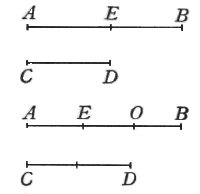
\includegraphics[width=5.00cm,height=4.85cm,keepaspectratio]{images/figura14.png} \end{center}
\end{center}

\speaker{Salv.} Sia questa linea \emph{AB} lo spazio e la dilatazione d'una vibrazione della corda grave, e la linea \emph{CD} quella della corda acuta, la quale con l'altra renda l'ottava, e dividasi la \emph{AB} in mezzo in \emph{E}: è manifesto, che cominciando a muoversi le corde nei termini \emph{A}, \emph{C}, quando la vibrazione acuta sarà pervenuta al termine \emph{D}, l'altra si sarà distesa solamente sino al mezzo \emph{E}, il quale, non sendo termine del moto, non percuote, ma ben si fa colpo in \emph{D}. Ritornando poi la vibrazione dal \emph{D} in \emph{C}, l'altra passa da \emph{E} in \emph{B}, onde le due percosse di \emph{B} e di \emph{C} battono unitamente su 'l timpano: e tornando a reiterarsi le simili seguenti vibrazioni, si concluderà, alternatamente in una sì e nell'altra no delle vibrazioni \emph{C}, \emph{D} accadere l'unione delle percosse con quelle di \emph{A}, \emph{B}. Ma le pulsazioni de i termini hanno sempre per compagne una delle \emph{C}, \emph{D}, e sempre la medesima: il che è manifesto; perché, posto che \emph{A}, \emph{C} battano insieme, nel passar \emph{A} in \emph{B}, \emph{C} va in \emph{D} e torna in \emph{C}, tal che \emph{C} batte con \emph{B}; e nel tempo che \emph{B} torna in \emph{A}, \emph{C} passa per \emph{D} e torna in \emph{C}, sì che i colpi \emph{A}, \emph{C} si fanno insieme. Ma sieno ora le due vibrazioni \emph{AB}, \emph{CD} quelle che producono la diapente, i tempi delle quali sono in proporzion sesquialtera, e dividasi la \emph{AB} della corda grave in tre parti eguali in \emph{E}, \emph{O}, e intendansi le vibrazioni cominciare nell'istesso momento da i termini \emph{A}, \emph{C}: è manifesto che nella percossa che si farà nel termine \emph{D}, la vibrazione di \emph{AB} sarà giunta solamente in \emph{O}; il timpano dunque riceve la percossa \emph{D} sola: nel ritorno poi da \emph{D} in \emph{C}, l'altra vibrazione passa da \emph{O} in \emph{B} e ritorna in \emph{O}, facendo la pulsazione in \emph{B}, che pure è sola e di contrattempo (accidente da considerarsi); perché, avendo poi posto le prime pulsazioni fatte nell'istesso momento nei termini \emph{A}, \emph{C}, la seconda, che fu sola del termine \emph{D}, si fece dopo quanto importa il tempo del transito \emph{CD}, cioè \emph{AO}, ma la seguente, che si fa in \emph{B}, dista dall'altra solo quanto è il tempo di \emph{OB}, che è la metà: continuando poi il ritorno da \emph{O} in \emph{A}, mentre da \emph{C} si va in \emph{D}, si viene a far le due pulsazioni unitamente in \emph{A} e \emph{D}. Seguono poi altri periodi simili a questi, cioè con l'interposizione di due pulsazioni della corda acuta, scompagnate e solitarie, e una della corda grave, pur solitaria e interposta tra le due solitarie dell'acuta. Sì che, se noi figureremo il tempo diviso in momenti, cioè in minime particole eguali; posto che nei due primi dalle concordi pulsazioni fatte in \emph{A}, \emph{C} si passi in \emph{O}, \emph{D}, e in \emph{D} si batta; che nel terzo e quarto momento si torni da \emph{D} in \emph{C}, battendo in \emph{C}, e che da \emph{O} si passi per \emph{B} e si torni in \emph{O}, battendosi in \emph{B}; e che finalmente nel quinto e sesto momento da \emph{O} e \emph{C} si passi in \emph{A} e \emph{D}, battendo in amendue; avremo sopra 'l timpano le pulsazioni distribuite con tal ordine, che poste le pulsazioni delle due corde nel medesimo instante, due momenti dopo riceverà una percossa solitaria, nel terzo momento un'altra pur solitaria, nel quarto un'altra sola, e due momenti dopo, cioè nel sesto, due congiunte insieme: e qui finisce il periodo, e, per dir così, l'anomalia, il qual periodo si va poi più volte replicando.

\speaker{Sagr.} Io non posso più tacere: è forza ch'io esclami il gusto che sento nel vedermi tanto adequatamente rese ragioni di effetti che tanto tempo m'hanno tenuto in tenebre e cecità. Ora intendo perché l'unisono non differisce punto da una voce sola: intendo perché l'ottava è la principal consonanza, ma tanto simile all'unisono, che come unisono si prende e si accompagna con le altre; simile è all'unisono, perché, dove le pulsazioni delle corde unisone vanno a ferire tutte insieme sempre, queste della corda grave dell'ottava vanno tutte accompagnate da quelle dell'acuta, e di queste una s'interpone solitaria ed in distanze eguali ed in certo modo senza fare scherzo alcuno, onde tal consonanza ne diviene sdolcinata troppo e senza brio. Ma la quinta, con quei suoi contrattempi, e con l'interpor tra le coppie delle due pulsazioni congiunte due solitarie della corda acuta ed una pur solitaria della grave, e queste tre con tanto intervallo di tempo quanto è la metà di quello che è tra ciascuna coppia e le solitarie dell'acuta, fa una titillazione ed un solletico tale sopra la cartilagine del timpano, che temperando la dolcezza con uno spruzzo d'acrimonia, par che insieme soavemente baci e morda.

\speaker{Salv.} È forza, poiché veggo che V. S. gusta tanto di queste novellizie, che io gli mostri il modo col quale l'occhio ancora, non pur l'udito, possa recrearsi nel veder i medesimi scherzi che sente l'udito. Sospendete palle di piombo, o altri simili gravi, da tre fili di lunghezze diverse, ma tali che nel tempo che il più lungo fa due vibrazioni, il più corto ne faccia quattro e 'l mezzano tre, il che accaderà quando il più lungo contenga sedici palmi o altre misure, delle quali il mezzano ne contenga nove ed il minore quattro; e rimossi tutti insieme dal perpendicolo e poi lasciatigli andare, si vedrà un intrecciamento vago di essi fili, con incontri varii, ma tali che ad ogni quarta vibrazione del più lungo tutti tre arriveranno al medesimo termine unitamente, e da quello poi si partiranno, reiterando di nuovo l'istesso periodo: la qual mistione di vibrazioni è quella che, fatta dalle corde, rende all'udito l'ottava con la quinta in mezzo. E se con simile disposizione si andranno temperando le lunghezze di altri fili, sì che le vibrazioni loro rispondano a quelle di altri intervalli musici, ma consonanti, si vedranno altri ed altri intrecciamenti, e sempre tali, che in determinati tempi e dopo determinati numeri di vibrazioni tutti i fili (siano tre o siano quattro) si accordano a giugner nell'istesso momento al termine di loro vibrazioni, e di lì a cominciare un altro simil periodo. Ma quando le vibrazioni di due o più fili siano o incommensurabili, sì che mai non ritornino a terminar concordemente determinati numeri di vibrazioni, o se pur, non essendo incommensurabili, vi ritornano dopo lungo tempo e dopo gran numero di vibrazioni, allora la vista si confonde nell'ordine disordinato di sregolata intrecciatura, e l'udito con noia riceve gli appulsi intemperati de i tremori dell'aria, che senza ordine o regola vanno a ferire su 'l timpano.

Ma dove, Signori miei, ci siamo lasciati trasportare per tante ore da i vani problemi ed inopinati discorsi? Siamo giunti a sera, e della proposta materia abbiamo trattato pochissimo o niente; anzi ce ne siamo in modo disviati, che a pena mi sovviene della prima introduzzione e di quel poco ingresso che facemmo come ipotesi e principio delle future dimostrazioni.

\speaker{Sagr.} Sarà dunque bene che ponghiamo per oggi fine a i nostri ragionamenti, dando commodo alla mente di andarsi nel riposo della notte tranquillando, per tornar poi domani (quando piaccia a V. S. di favorirci) a i discorsi desiderati e principalmente intesi.

\speaker{Salv.} Non mancherò d'esser qua all'istessa ora di oggi a servirle e goderle.


\vspace{1.5em}\begin{center}\large\itshape Finisce la prima Giornata\end{center}

\chapter*{Giornata Seconda}
\addcontentsline{toc}{chapter}{Giornata Seconda — Causa della coerenza e resistenza}
\markboth{Giornata Seconda}{Giornata Seconda}
\speaker{Sagr.} Stavamo, il Sig. Simplicio ed io, aspettando la venuta di V. S., e nel medesimo tempo ci andavamo riducendo a memoria l'ultima considerazione, che, quasi come principio e supposizione delle conclusioni che V. S. intendeva di dimostrarci, fu circa quella resistenza che hanno tutti i corpi solidi all'esser rotti, dependente da quel glutine che tiene le parti attaccate e congiunte, sì che non senza una potente attrazzione cedono e si separano. Si andò poi cercando qual potesse esser la causa di tal coerenza, che in alcuni solidi è gagliardissima, proponendosi principalmente quella del vacuo, che fu poi cagione di tante digressioni che ci tennero tutta la giornata occupati e lontani dalla materia primieramente intesa, che era, come ho detto, la contemplazione delle resistenze de i solidi all'essere spezzati.

\speaker{Salv.} Ben mi sovviene del tutto. E ritornando su 'l filo incominciato, posta qualunque ella sia la resistenza de i corpi solidi all'essere spezzati per una violenta attrazzione, basta che indubitabilmente ella in loro si trova; la quale, ben che grandissima contro alla forza di chi per diritto gli tira, minore per lo più si osserva nel violentargli per traverso: e così vegghiamo una verga, per esempio, d'acciaio o di vetro reggere per lo lungo il peso di mille libbre, che fitta a squadra in un muro si spezzerà con l'attaccargliene cinquanta solamente: e di questa seconda resistenza deviamo noi parlare, ricercando secondo quali proporzioni ella si ritrovi ne i prismi e cilindri simili o dissimili in figura e grossezza, essendo però dell'istessa materia. Nella quale specolazione io piglio come principio noto quello che nelle mecaniche si dimostra tra le passioni del vette, che noi chiamiamo leva, cioè che nell'uso della leva la forza alla resistenza ha la proporzion contraria di quella che hanno le distanze tra 'l sostegno e le medesime forza e resistenza.

\speaker{Simp.} Questo fu dimostrato da Aristotile, nelle sue Mecaniche, prima che da ogni altro.

\speaker{Salv.} Voglio che gli concediamo il primato nel tempo; ma nella fermezza della dimostrazione parmi che se gli deva per grand'intervallo anteporre Archimede, da una sola proposizione del quale, dimostrata da esso ne gli Equiponderanti, dependono le ragioni non solamente della leva, ma della maggior parte de gli altri strumenti mecanici.

\speaker{Sagr.} Ma già che questo principio è il fondamento di tutto quello che voi avete intenzione di volerci dimostrare, non sarebbe se non molto a proposito l'arrecarci anco la prova di tal supposizione, quando non sia materia molto prolissa, dandoci una intera e compita instruzzione.

\speaker{Salv.} Come questo si abbia a fare, sarà pur meglio che io per altro ingresso, alquanto diverso da quello d'Archimede, v'introduca nel campo di tutte le future specolazioni, e che non supponendo altro se non che pesi eguali posti in bilancia di braccia eguali facciano l'equilibrio (principio supposto parimente dal medesimo Archimede), io venga poi a dimostrarvi come non solamente altrettanto sia vero che pesi diseguali facciano l'equilibrio in stadera di braccia diseguali secondo la proporzione di essi pesi permutatamente sospesi, ma che l'istessa cosa fa colui che colloca pesi eguali in distanze eguali, che quello che colloca pesi diseguali in distanze che abbiano permutatamente la medesima proporzione che i pesi.


\begin{center}
\begin{center} 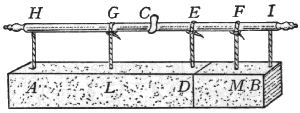
\includegraphics[width=7.50cm,height=2.83cm,keepaspectratio]{images/figura15.png} \end{center}
\end{center}

Or per chiara dimostrazione di quanto dico, segno un prisma o cilindro solido \emph{AB}, sospeso dall'estremità alla linea \emph{HI}, e sostenuto da due fili \emph{HA}, \emph{IB}: è manifesto, che se io sospenderò il tutto dal filo \emph{C}, posto nel mezzo della bilancia \emph{HI}, il prisma \emph{AB} resterà equilibrato, essendo la metà del suo peso da una banda, e l'altra dall'altra, del punto della sospensione \emph{C}, per il principio da noi supposto. Intendasi ora il prisma esser diviso in parti diseguali dal piano per la linea \emph{D}, e sia la parte \emph{DA} maggiore, e la \emph{DB} minore; ed acciò che, fatta tal divisione, le parti del prisma restino nel medesimo sito e costituzione rispetto alla linea \emph{HI}, soccorriamo con un filo \emph{ED}, il quale, fermato nel punto \emph{E}, sostenga le parti del prisma \emph{AD}, \emph{DB}; non è da dubitarsi che, non si essendo fatta veruna local mutazione nel prisma rispetto alla bilancia \emph{HI}, ella resterà nel medesimo stato dell'equilibrio. Ma nella medesima costituzione resterà ancora se la parte del prisma che ora è sospesa dalle due estremità con li fili \emph{AH}, \emph{DE}, si appenda ad un sol filo \emph{GL}, posto nel mezzo; e parimente l'altra parte \emph{DB} non muterà stato sospesa dal mezzo e sostenuta dal filo \emph{FM}: sciolti dunque i fili \emph{HA}, \emph{ED}, \emph{IB}, e lasciati solo li due \emph{GL}, \emph{FM}, resterà l'istesso equilibrio, fatta pur sempre la sospensione dal punto \emph{C}. Or qui voltiamoci a considerare come noi abbiamo due gravi \emph{AD}, \emph{DB}, pendenti da i termini \emph{G}, \emph{F} di una libra \emph{GF}, nella quale si fa l'equilibrio dal punto \emph{C}, in modo che la distanza della sospensione del grave \emph{AD} dal punto \emph{C} è la linea \emph{CG}, e l'altra parte \emph{CF} è la distanza dalla qual pende l'altro grave \emph{DB}: resta dunque solo da dimostrarsi, tali distanze aver la medesima proporzione tra di loro che hanno gli stessi pesi, ma permutatamente presi, cioè che la distanza \emph{GC} alla \emph{CF} sia come il prisma \emph{DB} al prisma \emph{DA}; il che proveremo così. Essendo la linea \emph{GE} la metà della \emph{EH}, e la \emph{EF} metà della \emph{EI}, sarà tutta la \emph{GF} metà di tutta la \emph{HI}, e però eguale alla \emph{CI}; e trattane la parte comune \emph{CF}, sarà la rimanente \emph{GC} eguale alla rimanente \emph{FI}, cioè alla \emph{FE}; e presa comunemente la \emph{CE}, saranno le due \emph{GE}, \emph{CF} eguali: e però, come \emph{GE} ad \emph{EF}, così \emph{FC} a \emph{CG}; ma come \emph{GE} ad \emph{EF}, così la doppia alla doppia, cioè \emph{HE} ad \emph{EI}, cioè il prisma \emph{AD} al prisma \emph{DB}; adunque, per l'egual proporzione e convertendo, come la distanza \emph{GC} alla distanza \emph{CF}, così il peso \emph{BD} al peso \emph{DA}: che è quello che io volevo provarvi.

Inteso sin qui, non credo che voi porrete difficoltà in ammettere che i due prismi \emph{AD}, \emph{DB} facciano l'equilibrio dal punto \emph{C}, perché la metà di tutto 'l solido \emph{AB} è alla destra della sospensione \emph{C}, e l'altra metà dalla sinistra, e che così si vengono a rappresentar due pesi eguali disposti e distesi in due distanze eguali. Che poi li due prismi \emph{AD}, \emph{DB} ridotti in due dadi, o in due palle, o in due qual'altre si siano figure (purché si conservino le sospensioni medesime \emph{G}, \emph{F}), seguitino di far l'equilibrio dal punto \emph{C}, non credo che sia alcuno che ne possa dubitare, perché troppo manifesta cosa è che le figure non mutano peso, dove si ritenga la medesima quantità di materia. Dal che possiamo raccor la general conclusione, che due pesi, qualunque si siano, fanno l'equilibrio da distanze permutatamente respondenti alle lor gravità.

Stabilito dunque tal principio, avanti che passiamo più oltre devo metter in considerazione come queste forze, resistenze, momenti, figure, etc., si posson considerar in astratto e separate dalla materia, ed anco in concreto e congiunte con la materia; ed in questo modo quelli accidenti che converranno alle figure considerate come immateriali, riceveranno alcune modificazioni mentre li aggiugneremo la materia, ed in consequenza la gravità.


\begin{center}
\begin{center} 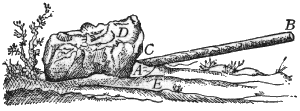
\includegraphics[width=7.50cm,height=2.78cm,keepaspectratio]{images/figura16.png} \end{center}
\end{center}

Come, per esempio, se noi intenderemo una leva, qual sarebbe questa \emph{BA}, la quale, posando su 'l sostegno \emph{E}, sia applicata per sollevare il grave sasso \emph{D}, è manifesto, per il dimostrato principio, che la forza posta nell'estremità \emph{B} basterà per adequare la resistenza del grave \emph{D}, se il suo momento al momento di esso \emph{D} abbia la medesima proporzione che ha la distanza \emph{AC} alla distanza \emph{CB}; e questo è vero, non mettendo in considerazione altri momenti che quelli della semplice forza in \emph{B} e della resistenza in \emph{D}, quasi che l'istessa leva fusse immateriale e senza gravità: ma se noi metteremo in conto la gravità ancora dello strumento stesso della leva, la quale sarà talor di legno e tal volta anco di ferro, è manifesto che, alla forza in \emph{B} aggiunto il peso della leva, altererà la proporzione, la quale converrà pronunziare sotto altri termini. E però, prima che passar più oltre, è necessario che noi convenghiamo in por distinzione tra queste due maniere di considerare, chiamando un \emph{prendere assolutamente} quello quando intenderemo lo strumento preso in astratto, cioè separato dalla gravità della propria materia; ma congiugnendo con le figure semplici ed assolute la materia, con la gravità ancora, nomineremo le figure congiunte con la materia \emph{momento} o \emph{forza composta}.

\speaker{Sagr.} È forza ch'io rompa il proposito che avevo di non dar occasione di digredire; ma non potrei con attenzione applicarmi al rimanente, se non mi fusse rimosso certo scrupolo che mi nasce; ed è questo: che mi pare che V. S. faccia comparazione della forza posta in \emph{B} con la total gravità del sasso \emph{D}, della qual gravità mi pare che una parte, e forse forse la maggiore, si appoggi sopra 'l piano dell'orizonte; sì che...

\speaker{Salv.} Ho inteso benissimo. V. S. non soggiunga altro ma solamente avverta che io non ho nominata la gravità totale del sasso, ma ho parlato del momento che egli tiene ed esercita sopra 'l punto \emph{A}, estremo termine della leva \emph{BA}; il quale è sempre minore dell'intero peso del sasso, ed è, variabile secondo la figura della pietra e secondo che ella vien più o meno sollevata.

\speaker{Sagr.} Resto appagato; ma mi nasce un altro desiderio, che è, che per intera cognizione mi fusse dimostrato il modo, se vi è, di poter investigare qual parte sia del peso totale quella che vien sostenuta dal soggetto piano, e quale quella che grava su 'l vette nell'estremità \emph{A}.

\speaker{Salv.} Perché posso con poche parole dargli sodisfazzione, non voglio lasciar di servirla. Però, facendone un poco di figura,


\begin{center}
\begin{center} 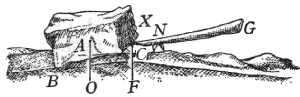
\includegraphics[width=7.50cm,height=2.43cm,keepaspectratio]{images/figura17.png} \end{center}
\end{center}

intenda V. S. il peso il cui centro di gravità sia \emph{A}, appoggiato sopra l'orizonte co 'l termine \emph{B}, e nell'altro sia sostenuto col vette \emph{CG}, sopra 'l sostegno \emph{N}, da una potenza posta in \emph{G}; e dal centro \emph{A} e dal termine \emph{C} caschino, perpendicolari all'orizzonte, \emph{AO}, \emph{CF}: dico, il momento di tutto il peso al momento della potenza in \emph{G} aver la proporzion composta della distanza \emph{GN} alla distanza \emph{NC} e della \emph{FB} alla \emph{BO}. Facciasi, come la linea \emph{FB} alla \emph{BO}, così la \emph{NC} alla \emph{X}: ed essendo tutto il peso \emph{A} sostenuto dalle due potenze poste in \emph{B} e \emph{C}, la potenza \emph{B} alla \emph{C} è come la distanza \emph{FO} alla \emph{OB}; e componendo, le due potenze \emph{B}, \emph{C} insieme, cioè il total momento di tutto 'l peso \emph{A}, alla potenza in \emph{C} è come la linea \emph{FB} alla \emph{BO}, cioè come la \emph{NC} alla \emph{X}: ma il momento della potenza in \emph{C} al momento della potenza in \emph{G} è come la distanza \emph{GN} alla \emph{NC}: adunque, per la perturbata, il total peso \emph{A} al momento della potenza in \emph{G} è come la \emph{GN} alla \emph{X}. Ma la proporzione di \emph{GN} ad \emph{X} è composta della proporzione di \emph{GN} ad \emph{NC} e di quella di \emph{NC} ad \emph{X}, cioè di \emph{FB} a \emph{BO}; adunque il peso \emph{A} alla potenza che lo sostiene in \emph{G} ha la proporzione composta della \emph{GN} ad \emph{NC} e di quella di \emph{FB} a \emph{BO}: ch'è quello che si doveva dimostrare.


\propbox{Prop I}

Or tornando al nostro primo proposito, intese tutte le cose sin qui dichiarate, non sarà difficile l'intender la ragione onde avvenga che un prisma o cilindro solido, di vetro, acciaio, legno o altra materia frangibile, che sospeso per lungo sosterrà gravissimo peso che gli sia attaccato, ma in traverso (come poco fa dicevamo) da minor peso assai potrà tal volta essere spezzato, secondo che la sua lunghezza eccederà la sua grossezza.


\begin{center}
\begin{center} 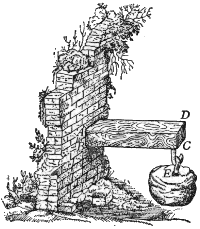
\includegraphics[width=5.00cm,height=5.73cm,keepaspectratio]{images/figura18.png} \end{center}
\end{center}

Imperò che figuriamoci il prisma solido \emph{ABCD}, fitto in un muro dalla parte \emph{AB}, e nell'altra estremità s'intenda la forza del peso \emph{E} (intendendo sempre, il muro esser eretto all'orizonte, ed il prisma o cilindro fitto nel muro ad angoli retti): è manifesto che, dovendosi spezzare, si romperà nel luogo \emph{B}, dove il taglio del muro serve per sostegno, e la \emph{BC} per la parte della leva dove si pone la forza; e la grossezza del solido \emph{BA} è l'altra parte della leva, nella quale è posta la resistenza, che consiste nello staccamento che s'ha da fare della parte del solido \emph{BD}, che è fuor del muro, da quella che è dentro: e per le cose dichiarate, il momento della forza posta in \emph{C} al momento della resistenza, che sta nella grossezza del prisma cioè nell'attaccamento della base \emph{BA} con la sua contigua, ha la medesima proporzione che la lunghezza \emph{CB} alla metà della \emph{BA}; e però l'assoluta resistenza all'esser rotto, che è nel prisma \emph{BD} (la quale assoluta resistenza è quella che si fa col tirarlo per diritto, perché allora tanto è il moto del movente quanto quello del mosso), all'esser rotto con l'aiuto della leva \emph{BC}, ha la medesima proporzione che la lunghezza \emph{BC} alla metà di \emph{AB} nel prisma, che nel cilindro è il semidiametro della sua base. E questa sia la nostra prima proposizione. E notate, che questo che dico, si debbe intendere, rimossa la considerazione del peso proprio del solido \emph{BD}, il qual solido ho preso come nulla pesante: ma quando vorremo mettere in conto la sua gravità, congiugnendola col peso \emph{E}, doviamo al peso \emph{E} aggiugnere la metà del peso del solido \emph{BD}; sì che essendo, v. g., il peso di \emph{BD} due libbre, e 'l peso di \emph{E} libbre dieci, si deve pigliare il peso \emph{E} come se fusse undici.

\speaker{Simp.} E perché non come se fusse dodici?

\speaker{Salv.} Il peso \emph{E}, Sig. Simplicio mio, pendente dal termine \emph{C}, preme, in rispetto alla leva \emph{BC}, con tutto 'l suo momento di libbre dieci; dove se fusse appeso il solo \emph{BD}, graverebbe con tutto 'l momento di due libbre: ma, come vedete, tal solido è distribuito per tutta la lunghezza \emph{BC} uniformemente, onde le parti sue vicine all'estremità \emph{B} gravano manco delle più remote; sì che in somma, ristorando quelle con queste, il peso di tutto 'l prisma si riduce a lavorare sotto 'l centro della sua gravità, che risponde al mezzo della leva \emph{BC}: ma un peso pendente dalla estremità \emph{C} ha momento doppio di quello che arebbe pendendo dal mezzo: e però la metà del peso del prisma si deve aggiugnere al peso \emph{E}, mentre ci serviamo del momento di amendue, come locati nel termine \emph{C}.

\speaker{Simp.} Resto capacissimo; e di più, s'io non m'inganno, parmi che la potenza di amendue i pesi \emph{BD} ed \emph{E}, posti così, arebbe l'istesso momento che se tutto il peso di \emph{BD} col doppio di \emph{E} fusse appeso nel mezo della leva \emph{BC}.


\propbox{Prop II}

\speaker{Salv.} Così è precisamente, e si deve tenere a memoria. Qui possiamo immediatamente intender, come e con che proporzione resista più una verga, o vogliam dir prisma più largo che grosso, all'esser rotto, fattogli forza secondo la sua larghezza, che secondo la grossezza.


\begin{center}
\begin{center} 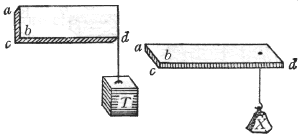
\includegraphics[width=7.50cm,height=3.43cm,keepaspectratio]{images/figura19.png} \end{center}
\end{center}

Per intelligenza di che, intendasi una riga \emph{ad}, la cui larghezza sia \emph{ac}, e la grossezza, assai minore, \emph{cb}: si cerca perché, volendola romper per taglio, come nella prima figura, resisterà al gran peso \emph{T}; ma posta per piatto, come nella seconda figura, non resisterà all'\emph{X}, minore del \emph{T}. Il che si fa manifesto, mentre intendiamo, il sostegno essere una volta sotto la linea \emph{bc}, ed un'altra sotto la \emph{ca}, e le distanze delle forze esser nell'un caso e nell'altro eguali, cioè la lunghezza \emph{bd}; ma nel primo caso la distanza della resistenza dal sostegno, che è la metà della linea \emph{ca}, è maggiore della distanza nell'altro caso, la quale è la metà della \emph{bc}; però la forza del peso \emph{T} conviene che sia maggiore della \emph{X} quanto la metà della larghezza \emph{ca} è maggiore della metà della grossezza \emph{bc}, servendoci quella per contralleva della \emph{ca}, e questa della \emph{cb}, per superare la medesima resistenza, che è la quantità delle fibre di tutta la base \emph{ab}. Concludesi per tanto, la medesima riga o prisma più largo che grosso resister più all'esser rotto per taglio che per piatto, secondo la proporzione della larghezza alla grossezza.


\propbox{Prop III}

Conviene ora che cominciamo a investigare secondo qual proporzione vadia crescendo il momento della propria gravità, in relazione alla propria resistenza all'essere spezzato in un prisma o cilindro, mentre, stando parallelo all'orizonte, si va allungando; il qual momento trovo andar crescendo in duplicata proporzione di quella dell'allungamento.


\begin{center}
\begin{center} 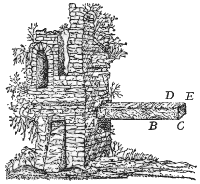
\includegraphics[width=5.00cm,height=4.60cm,keepaspectratio]{images/figura20.png} \end{center}
\end{center}

Per la cui dimostrazione, intendasi il prisma o cilindro \emph{AD} fitto saldamente nel muro dall'estremità \emph{A}, e sia equidistante all'orizonte; ed il medesimo intendasi allungato sino in \emph{E}, aggiugnendovi la parte \emph{BE}. È manifesto che l'allungamento della leva \emph{AB} sino in \emph{C} cresce per sé solo, cioè assolutamente preso, il momento della forza premente contro alla resistenza dello staccamento e rottura da farsi in \emph{A} secondo la proporzione di \emph{CA} e \emph{BA}: ma, oltre a questo, il peso aggiunto del solido \emph{BE} al peso del solido \emph{AB} cresce il momento della gravità premente secondo la proporzione del prisma \emph{AE} al prisma \emph{AB}, la qual proporzione è la medesima della lunghezza \emph{AC} alla \emph{AB}: adunque è manifesto che, congiunti i due accrescimenti delle lunghezze e delle gravità, il momento composto di amendue è in doppia proporzione di qualunque di esse. Concludasi per tanto, i momenti delle forze de i prismi e cilindri egualmente grossi, ma disegualmente lunghi, esser tra di loro in duplicata proporzione di quella delle lor lunghezze, cioè esser come i quadrati delle lunghezze.

Mostreremo adesso, nel secondo luogo, secondo qual proporzione cresca la resistenza all'essere spezzati ne i prismi e cilindri, mentre restino della medesima lunghezza e si accresca la grossezza. E qui dico che:


\propbox{Prop IV}

Ne i prismi e cilindri egualmente lunghi, ma disegualmente grossi, la resistenza all'esser rotti cresce in triplicata proporzione de i diametri delle lor grossezze, cioè delle lor basi.


\begin{center}
\begin{center} 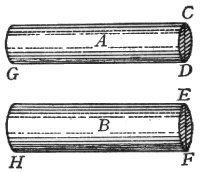
\includegraphics[width=5.00cm,height=4.30cm,keepaspectratio]{images/figura21.png} \end{center}
\end{center}

I due cilindri siano questi \emph{A}, \emph{B}; le cui lunghezze eguali, \emph{DG}, \emph{FH}; le basi diseguali, i cerchi i cui diametri \emph{CD}, \emph{EF}: dico, la resistenza del cilindro \emph{B} alla resistenza del cilindro \emph{A}, ad esser rotti, aver triplicata proporzione di quella che ha il diametro \emph{FE} al diametro \emph{DC}. Imperò che, se consideriamo l'assoluta e semplice resistenza che risiede nelle basi, cioè ne i cerchi \emph{EF}, \emph{DC}, all'essere strappati facendogli forza col tirargli per diritto, non è dubbio che la resistenza del cilindro \emph{B} è tanto maggiore che quella del cilindro \emph{A}, quanto il cerchio \emph{EF} è maggiore del \emph{CD}, perché tante più sono le fibre, i filamenti o le parti tenaci, che tengono unite le parti de i solidi. Ma se consideriamo che nel far forza per traverso ci serviamo di due leve, delle quali le parti o distanze dove si applicano le forze sono le linee \emph{DG}, \emph{FH}, i sostegni sono ne' punti \emph{D}, \emph{F}, ma le altre parti o distanze dove son poste le resistenze sono i semidiametri de i cerchi \emph{DC}, \emph{EF}, perché i filamenti sparsi per tutte le superficie de i cerchi è come se tutti si riducessero ne i centri; considerando, dico, tali leve, intenderemo, la resistenza nel centro della base \emph{EF} contro alla forza di \emph{H} esser tanto maggiore della resistenza della base \emph{CD} contro alla forza posta in \emph{G} (e sono le forze in \emph{G} ed \emph{H} di leve uguali \emph{DG}, \emph{FH}), quanto il semidiametro \emph{FE} è maggiore del semidiametro \emph{DC}. Cresce dunque la resistenza all'esser rotto nel cilindro \emph{B} sopra la resistenza del cilindro \emph{A} secondo amendue le proporzioni de i cerchi \emph{EF}, \emph{DC} e de i lor semidiametri, o vogliam dir diametri: ma la proporzione de i cerchi è doppia di quella de i diametri: adunque la proporzione delle resistenze, che di quelle si compone, è triplicata della proporzione de i medesimi diametri: che è quello che dovevo provare. Ma perché anco i cubi sono in tripla proporzione de i loro lati, possiamo similmente concludere, le resistenze de i cilindri egualmente lunghi esser tra di loro come i cubi de i lor diametri.


\propbox{Corol.}

Da questo che si è dimostrato possiamo concludere ancora, le resistenze de i prismi e cilindri egualmente lunghi aver sesquialtera proporzione di quella de gli stessi cilindri. Il che è manifesto: perché i prismi e cilindri egualmente alti hanno fra di loro la medesima proporzione che le lor basi, cioè doppia de i lati o diametri di esse basi; ma le resistenze (come si è dimostrato) hanno triplicata proporzione de i medesimi lati o diametri; adunque la proporzione delle resistenze è sesquialtera della proporzione de gli stessi solidi, ed in consequenza de i pesi de i medesimi solidi.

\speaker{Simp.} Egli è forza che, avanti che si proceda più oltre, io resti sincerato di certa mia difficoltà. E questa è, che sin qui non ho sentito mettere in considerazione cert'altra sorte di resistenza, la quale mi par che venga diminuita ne i solidi secondo che si vanno più e più allungando, e non solo nell'uso trasversale, ma ancora per lo lungo; in quel modo appunto che veggiamo, una corda lunghissima esser molto meno atta a reggere un gran peso, che se fusse corta: onde io credo che una verga di legno o di ferro più peso assai potrà reggere se sarà corta, che se sarà molto lunga; intendendo sempre usata per lo lungo, e non in traverso, ed anco messo in conto il suo proprio peso, che nella più lunga è maggiore.

\speaker{Salv.} Dubito, Sig. Simplicio, che in questo punto voi, con molti altri, v'inganniate, se però ho ben compreso il vostro concetto, sì che voi vogliate dire che una corda lunga, v. g., quaranta braccia non possa sostenere tanto peso, quanto se fusse un braccio o due della medesima corda.

\speaker{Simp.} Cotesto ho voluto dire, e sin qui mi par proposizione assai probabile.

\speaker{Salv.} Ma io l'ho per falsa, non che per improbabile; e credo di potervi assai agevolmente cavar d'errore.


\begin{center}
\begin{center} 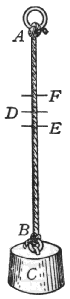
\includegraphics[width=1.75cm,height=7.48cm,keepaspectratio]{images/figura22.png} \end{center}
\end{center}

Però ponghiamo questa corda \emph{AB}, fermata di sopra dal capo \emph{A}, e dall'altro sia il peso \emph{C}, dalla cui forza debba essa corda essere rotta: assegnatemi voi, Sig. Simplicio, il luogo particolare dove debba seguir la rottura.

\speaker{Simp.} Sia nel luogo \emph{D}.

\speaker{Salv.} Vi domando qual sia la cagione dello strapparsi in \emph{D}.

\speaker{Simp.} È la causa di ciò, perché la corda in quella parte non era potente a reggere, v. g., cento libbre di peso, quanto è la parte \emph{DB} con la pietra C.

\speaker{Salv.} Adunque, tutta volta che tal corda nella parte \emph{D} venisse violentata dalle medesime cento libbre di peso, ella li si strapperebbe.

\speaker{Simp.} Così credo.

\speaker{Salv.} Ma ditemi ora: chi attaccasse il medesimo peso non al fine della corda \emph{B}, ma vicino al punto \emph{D}, come sarebbe in \emph{E}, o vero legasse la corda non nella altezza \emph{A}, ma più vicina e sopra al punto medesimo \emph{D}, come sarebbe in \emph{F}, ditemi, dico, se il punto \emph{D} sentirebbe il medesimo peso delle cento libbre.

\speaker{Simp.} Sentirebbelo, accompagnando però il pezzo di corda \emph{EB} con la pietra \emph{C}.

\speaker{Salv.} Se dunque la corda nel punto \emph{D} vien tirata dalle medesime cento libbre di peso, si romperà, per la vostra concessione: e pure la \emph{FE} è un piccol pezzo della lunga \emph{AB}; come dunque volete più dire che la corda lunga sia più debole della corta? Contentatevi dunque d'esser cavato d'un errore nel quale avete auto molti compagni, ed anco per altro molto intelligenti, e seguitiamo innanzi. Ed avendo dimostrato, i prismi e cilindri crescere il lor momento sopra le proprie resistenze secondo i quadrati delle lunghezze loro (mantenendo però sempre la medesima grossezza); e parimente, gli egualmente lunghi, ma differenti in grossezza, crescer le lor resistenze secondo la proporzione de i cubi de i lati o diametri delle lor basi, passiamo a investigare quello che accaggia a tali solidi differenti in lunghezza e grossezza insieme. Ne i quali io osservo che:


\propbox{Prop. V}

I prismi e cilindri di diversa lunghezza e grossezza hanno le lor resistenze all'esser rotti di proporzione composta della proporzione de i cubi de' diametri delle lor basi e della proporzione delle lor lunghezze permutatamente prese.


\begin{center}
\begin{center} 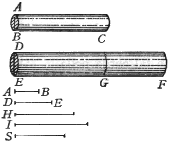
\includegraphics[width=4.25cm,height=3.60cm,keepaspectratio]{images/figura23.png} \end{center}
\end{center}

Siano tali due cilindri \emph{ABC}, \emph{DEF}: dico, la resistenza del cilindro \emph{AC} alla resistenza del cilindro \emph{DF} aver la proporzione composta della proporzione del cubo del diametro \emph{AB} al cubo del diametro \emph{DE} e della proporzione della lunghezza \emph{EF} alla lunghezza \emph{BC}. Pongasi la \emph{EG} eguale alla \emph{BC}, e delle linee \emph{AB}, \emph{DE} sia terza proporzionale la \emph{H}, e quarta la \emph{I}, e come la \emph{EF} alla \emph{BC} così sia la \emph{I} alla \emph{S}. E perché la resistenza del cilindro \emph{AC} alla resistenza del cilindro \emph{DG} è come il cubo \emph{AB} al cubo \emph{DE}, cioè come la linea \emph{AB} alla linea \emph{I}; e la resistenza del cilindro \emph{DG} alla resistenza del cilindro \emph{DF} come la lunghezza \emph{FE} alla \emph{EG}, cioè come la linea \emph{I} alla \emph{S}; adunque, per l'egual proporzione come la resistenza del cilindro \emph{AC} alla resistenza del cilindro \emph{DF}, così la linea \emph{AB} alla \emph{S}: ma la linea \emph{AB} alla \emph{S} ha la proporzion composta della \emph{AB} alla \emph{I} e della \emph{I} alla S: adunque la resistenza del cilindro \emph{AC} alla resistenza del cilindro \emph{DF} ha la proporzion composta della \emph{AB} alla \emph{I}, cioè del cubo di \emph{AB} al cubo di \emph{DE}, e della proporzione della linea \emph{I} alla \emph{S}, cioè della lunghezza \emph{EF} alla lunghezza \emph{BC}: che è quello che intendevo di dimostrare.

Dopo la dimostrata proposizione, voglio che consideriamo quello che accaggia tra i cilindri e prismi simili: de i quali dimostreremo come:


\propbox{Prop. VI}

De i cilindri e prismi simili i momenti composti, cioè risultanti dalle lor gravità e dalle loro lunghezze, che sono come leve, hanno tra di loro proporzione sesquialtera di quella che hanno le resistenze delle medesime lor basi.


\begin{center}
\begin{center} 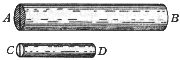
\includegraphics[width=4.50cm,height=1.50cm,keepaspectratio]{images/figura24.png} \end{center}
\end{center}

Per il che dimostrare, segniamo i due cilindri simili \emph{AB}, \emph{CD}: dico, il momento del cilindro \emph{AB} per superare la resistenza della sua base \emph{B}, al momento di \emph{CD} per superare la resistenza della sua \emph{D}, aver sesquialtera proporzione di quella che ha la medesima resistenza della base \emph{B} alla resistenza della base \emph{D}. E perché i momenti de i solidi \emph{AB}, \emph{CD} per superar le resistenze delle lor basi \emph{B}, \emph{D} son composti delle lor gravità e delle forze delle lor leve, e la forza della leva \emph{AB} è eguale alla forza della leva \emph{CD} (e questo perché la lunghezza \emph{AB} al semidiametro della base \emph{B} ha la medesima proporzione, per la similitudine de' cilindri, che la lunghezza \emph{CD} al semidiametro della base \emph{D}), resta che 'l momento totale del cilindro \emph{AB} al momento totale di \emph{CD} sia come la sola gravità del cilindro \emph{AB} alla sola gravità del cilindro \emph{CD}, cioè come l'istesso cilindro \emph{AB} all'istesso \emph{CD}; ma questi sono in triplicata proporzione de i diametri delle basi loro \emph{B}, \emph{D}; e le resistenze delle medesime basi, essendo tra di loro come l'istesse basi, sono, in consequenza, in duplicata proporzione de i medesimi loro diametri: adunque i momenti de i cilindri son in sesquialtera proporzione delle resistenze delle basi loro.

\speaker{Simp.} Questa proposizione mi è veramente giunta non solamente nuova, ma inaspettata, e nel primo aspetto assai remota dal giudizio che io ne averei conietturalmente fatto: imperò che, essendo tali figure in tutto 'l restante simili, arei tenuto per fermo che anco i momenti loro verso le proprie resistenze avessero ritenuta la medesima proporzione.

\speaker{Sagr.} Questa è la dimostrazione di quella proposizione, che nel principio de' nostri ragionamenti dissi parermi di scorger per ombra.

\speaker{Salv.} Quello che ora accade al Sig. Simplicio, avvenne per alcun tempo a me, credendo che le resistenze di solidi simili fusser simili, sin che certa, né anco molto fissa o accurata, osservazione mi pareva rappresentarmi, ne i solidi simili non mantenersi un tenore eguale nelle loro robustezze, ma i maggiori esser meno atti a patire gl'incontri violenti, come rimaner più offesi dalle cadute gli uomini grandi che i piccoli fanciulli; e, come da principio dicevamo, cadendo dalla medesima altezza vedesi andare in pezzi una gran trave o una colonna, ma non così un piccolo corrente o un piccol cilindro di marmo. Questa tal quale osservazione mi destò la mente all'investigazione di quello che ora son per dimostrarvi: proprietà veramente ammirabile, poiché tra le infinite figure solide simili tra di loro, pur due non ve ne sono, i momenti delle quali verso le proprie resistenze ritenghino la medesima proporzione.

\speaker{Simp.} Ora mi fate sovvenire non so che, posto da Aristotele tra le sue Quistioni Mecaniche, mentre vuol render la ragione onde avvenga che i legni, quanto più son lunghi, tanto più son deboli e più si piegano, ben che i più corti sieno più sottili, e i lunghi più grossi; e se io ben mi ricordo, ne riduce la ragione alla semplice leva.

\speaker{Salv.} È verissimo: e perché la soluzione non par che tolga interamente la ragion del dubitare, Monsig. di Guevara, il quale veramente con i suoi dottissimi comentarii ha altamente nobilitata e illustrata quell'opera, si estende con altre più acute specolazioni per sciorre tutte le difficoltà, restando però esso ancora perplesso in questo punto, se crescendosi con la medesima proporzione le lunghezze e le grossezze di tali solide figure, si deva mantenere l'istesso tenore nelle loro robustezze e resistenze nell'esser rotte ed anco nel piegarsi. Io, dopo un lungo pensarvi, ho in questa materia ritrovato quello che seguentemente son per apportarvi. E prima dimostrerò che:


\propbox{Prop. VII}

De i prismi o cilindri simili gravi, un solo e unico è quello che si riduce (gravato dal proprio peso) all'ultimo stato tra lo spezzarsi e 'l sostenersi intero: sì che ogni maggiore, come impotente a resistere al proprio peso, si romperà; e ogni minore resiste a qualche forza che gli venga fatta per romperlo.


\begin{center}
\begin{center} 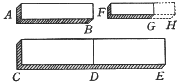
\includegraphics[width=4.50cm,height=2.10cm,keepaspectratio]{images/figura25.png} \end{center}
\end{center}

Sia il prisma grave \emph{AB} ridotto alla somma lunghezza di sua consistenza, sì che allungato un minimo di più si rompesse: dico, questo esser unico tra tutti i suoi simili (che pur sono infiniti); atto ad esser ridotto in tale stato ancipite; sì che ogni maggiore, oppresso dal proprio peso, si spezzerà, ed ogni minore no, anzi potrà resistere a qualche aggravio di nuova violenza, oltre a quella del proprio peso. Sia prima il prisma \emph{CE}, simile e maggiore di \emph{AB}: dico, questo non poter consistere, ma rompersi, superato dalla propria gravità. Pongasi la parte \emph{CD} lunga quanto \emph{AB}: e perché la resistenza di \emph{CD} a quella di \emph{AB} è come il cubo della grossezza di \emph{CD} al cubo della grossezza di \emph{AB}, cioè come il prisma \emph{CE} al prisma \emph{AB} (essendo simili), adunque il peso di \emph{CE} è il sommo che possa esser sostenuto nella lunghezza del prisma \emph{CD}; ma la lunghezza \emph{CE} è maggiore; adunque il prisma \emph{CE} si romperà. Ma sia \emph{FG} minore: si dimostrerà similmente (posta \emph{FH} eguale alla \emph{BA}), la resistenza di \emph{FG} a quella di \emph{AB} esser come il prisma \emph{FG} al prisma \emph{AB}, quando la distanza \emph{AB}, cioè \emph{FH}, fusse eguale alla \emph{FG}; ma è maggiore; adunque il momento del prisma \emph{FG} posto in \emph{G} non basta per romper il prisma \emph{FG}.

\speaker{Sagr.} Chiarissima e breve dimostrazione, concludente la verità e necessità di una proposizione che, nel primo aspetto, sembra assai remota dal verisimile. Bisognerebbe dunque alterare assai la proporzione tra la lunghezza e la grossezza del prisma maggiore, con l'ingrossarlo o scorciarlo, acciò si riducesse allo stato ancipite tra 'l reggersi e lo spezzarsi; e l'investigazione di tale stato penso che potesse esser altrettanto ingegnosa.

\speaker{Salv.} Anzi più presto d'avvantaggio, come anco più laboriosa; ed io lo so, che vi spesi non piccol tempo per ritrovarla, ed ora voglio participarvela.


\propbox{Prop. VIII}

Dato dunque un cilindro o prisma di massima lunghezza da non esser dal suo proprio peso spezzato, e data una lunghezza maggiore, trovar la grossezza d'un altro cilindro o prisma che sotto la data lunghezza sia l'unico e massimo resistente al proprio peso.


\begin{center}
\begin{center} 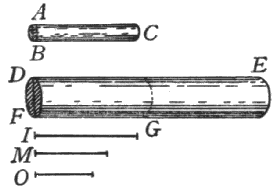
\includegraphics[width=7.00cm,height=4.83cm,keepaspectratio]{images/figura26.png} \end{center}
\end{center}

Sia il cilindro \emph{BC} massimo resistente al proprio peso, e sia la \emph{DE} lunghezza maggiore della \emph{AC}: bisogna trovare la grossezza del cilindro che sotto la lunghezza \emph{DE} sia il massimo resistente al proprio peso. Sia delle lunghezze \emph{DE}, \emph{AC} terza proporzionale \emph{I}, e come \emph{DE} ad \emph{I}, così sia il diametro \emph{FD} al diametro \emph{BA}, e facciasi il cilindro \emph{FE}; dico, questo esser il massimo ed unico, tra tutti i suoi simili, resistente al proprio peso. Delle linee \emph{DE}, \emph{I} sia terza proporzionale \emph{M}, e quarta \emph{O}, e pongasi \emph{FG} eguale alla \emph{AC}: e perché il diametro \emph{FD} al diametro \emph{AB} è come la linea \emph{DE} alla \emph{I}, e delle \emph{DE}, \emph{I} la \emph{O} è quarta proporzionale, il cubo di \emph{FD} al cubo di \emph{BA} sarà come la \emph{DE} alla \emph{O}; ma come il cubo di \emph{FD} al cubo di \emph{BA}, così è la resistenza del cilindro \emph{DG} alla resistenza del cilindro \emph{BC}; adunque la resistenza del cilindro \emph{DG} a quella del cilindro \emph{BC} è come la linea \emph{DE} alla \emph{O}. E perché il momento del cilindro \emph{BC} è eguale alla sua resistenza, se si mostrerà, il momento del cilindro \emph{FE} al momento del cilindro \emph{BC} esser come la resistenza \emph{DF} alla resistenza \emph{BA}, cioè come il cubo di \emph{FD} al cubo di \emph{BA}, cioè come la linea \emph{DE} alla \emph{O}, aremo l'intento, cioè il momento del cilindro \emph{FE} esser eguale alla resistenza posta in \emph{FD}. Il momento del cilindro \emph{FE} al momento del cilindro \emph{DG} è come il quadrato della \emph{DE} al quadrato della \emph{AC}, cioè come la linea \emph{DE} alla \emph{I}; ma il momento del cilindro \emph{DG} al momento del cilindro \emph{BC} è come il quadrato \emph{DF} al quadrato \emph{BA}, cioè come il quadrato di \emph{DE} al quadrato della \emph{I}, cioè come il quadrato della \emph{I} al quadrato della \emph{M}, cioè come la \emph{I} alla \emph{O}; adunque, per l'egual proporzione, come il momento del cilindro \emph{FE} al momento del cilindro \emph{BC}, così è la linea \emph{DE} alla \emph{O}, cioè il cubo \emph{DF} al cubo \emph{BA}, cioè la resistenza della base \emph{DF} alla resistenza della base \emph{BA}: che è quello che si cercava.

\speaker{Sagr.} Questa, Sig. Salviati, è una lunga dimostrazione, e molto difficile a ritenersi a memoria per sentirla una sola volta; onde io vorrei che V. S. si contentasse di replicarla di nuovo.

\speaker{Salv.} Farò quanto V. S. comanda; ma forse sarebbe meglio arrecarne una più speditiva e breve: ma converrà fare una figura alquanto diversa.

\speaker{Sagr.} Maggiore sarà il favore; e la già dichiarata mi farà grazia darmela scritta, acciò a mio bell'agio possa ristudiarla.

\speaker{Salv.} Non mancherò di servirla.


\begin{center}
\begin{center} 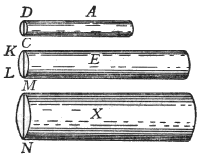
\includegraphics[width=5.00cm,height=3.95cm,keepaspectratio]{images/figura27.png} \end{center}
\end{center}

Ora intendiamo un cilindro \emph{A}, il diametro della cui base sia la linea \emph{DC}, e sia questo \emph{A} il massimo che possa sostenersi; del quale vogliamo trovare un maggiore, che pur sia il massimo esso ancora ed unico che si sostenga. Intendiamone un simile ad esso \emph{A} e lungo quanto la linea assegnata, e questo sia, v. g., \emph{E}, il diametro della cui base sia la \emph{KL}, e delle due linee \emph{DC}, \emph{KL} sia terza proporzionale la \emph{MN}, che sia diametro della base del cilindro \emph{X}, di lunghezza eguale all'\emph{E}: dico, questo \emph{X} esser quello che cerchiamo. E perché la resistenza \emph{DC} alla resistenza \emph{KL} è come il quadrato \emph{DC} al quadrato \emph{KL}, cioè come il quadrato \emph{KL} al quadrato \emph{MN}, cioè come il cilindro \emph{E} al cilindro \emph{X}, cioè come il momento \emph{E} al momento \emph{X}; ma la resistenza \emph{KL} alla \emph{MN} è come il cubo di \emph{KL} al cubo di \emph{MN}, cioè come il cubo \emph{DC} al cubo \emph{KL}, cioè come il cilindro \emph{A} al cilindro \emph{E}, cioè come il momento \emph{A} al momento \emph{E}; adunque, per l'analogia perturbata, come la resistenza \emph{DC} alla \emph{MN}, così il momento \emph{A} al momento \emph{X}: adunque il prisma \emph{X} è nella medesima costituzione di momento e resistenza che il prisma \emph{A}.

Ma voglio che facciamo il problema più generale; e la proposizione sia questa:


\begin{enunciato}
Dato il cilindro \emph{AC}, qualunque si sia il suo momento verso la sua resistenza, e data qual si sia lunghezza \emph{DE}, trovar la grossezza del cilindro, la cui lunghezza sia \emph{DE}, e 'l suo momento verso la sua resistenza ritenga la medesima proporzione che il momento del cilindro \emph{AC} alla sua.
\end{enunciato}

Ripresa l'istessa figura di sopra e quasi l'istesso progresso, diremo: perché il momento del cilindro \emph{FE} al momento della parte \emph{DG} ha la medesima proporzione che il quadrato \emph{ED} al quadrato \emph{FG}, cioè che la linea \emph{DE} alla \emph{I}; ed il momento del cilindro \emph{FG} al momento del cilindro \emph{AC} è come il quadrato \emph{FD} al quadrato \emph{AB}, cioè come il quadrato \emph{DE} al quadrato \emph{I}, cioè come il quadrato \emph{I} al quadrato \emph{M}, cioè come la linea \emph{I} alla \emph{O}; adunque \emph{ex æquali}, il momento del cilindro \emph{FE} al momento del cilindro \emph{AC} ha la medesima proporzione della linea \emph{DE} alla \emph{O}, cioè del cubo \emph{DE} al cubo \emph{I}, cioè del cubo di \emph{FD} al cubo di \emph{AB}, cioè della resistenza della base \emph{FD} alla resistenza della base \emph{AB}: ch'è quello che si doveva fare.

Or vegghino come dalle cose sin qui dimostrate apertamente si raccoglie l'impossibilità del poter non solamente l'arte, ma la natura stessa, crescer le sue macchine a vastità immensa: sì che impossibil sarebbe fabbricar navilii, palazzi o templi vastissimi, li cui remi, antenne, travamenti, catene di ferro, ed in somma le altre lor parti, consistessero; come anco non potrebbe la natura far alberi di smisurata grandezza, poiché i rami loro, gravati dal proprio peso, finalmente si fiaccherebbero; e parimente sarebbe impossibile far strutture di ossa per uomini, cavalli o altri animali, che potessero sussistere e far proporzionatamente gli uffizii loro, mentre tali animali si dovesser agumentare ad altezze immense, se già non si togliesse materia molto più dura e resistente della consueta, o non si deformassero tali ossi, sproporzionatamente ingrossandogli, onde poi la figura ed aspetto dell'animale ne riuscisse mostruosamente grosso: il che forse fu avvertito dal mio accortissimo Poeta, mentre descrivendo un grandissimo gigante disse:


\begin{enunciato}
Non si può compatir quanto sia lungo, \\ Sì smisuratamente è tutto grosso.
\end{enunciato}

E per un breve esempio di questo che dico, disegnai già la figura di un osso allungato solamente tre volte, ed ingrossato con tal proporzione, che potesse nel suo animale grande far l'uffizio proporzionato a quel dell'osso minore nell'animal più piccolo, e le figure son queste:


\begin{center}
\begin{center} 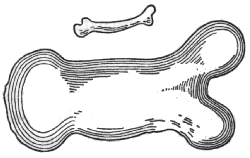
\includegraphics[width=6.25cm,height=3.95cm,keepaspectratio]{images/figura28.png} \end{center}
\end{center}

dove vedete sproporzionata figura che diviene quella dell'osso ingrandito. Dal che è manifesto, che chi volesse mantener in un vastissimo gigante le proporzioni che hanno le membra in un uomo ordinario, bisognerebbe o trovar materia molto più dura e resistente, per formarne l'ossa, o vero ammettere che la robustezza sua fusse a proporzione assai più fiacca che ne gli uomini di statura mediocre; altrimente, crescendogli a smisurata altezza, si vedrebbono dal proprio peso opprimere e cadere. Dove che, all'incontro, si vede, nel diminuire i corpi non si diminuir con la medesima proporzione le forze, anzi ne i minimi crescer la gagliardia con proporzion maggiore: onde io credo che un piccolo cane porterebbe addosso due o tre cani eguali a sé, ma non penso già che un cavallo portasse né anco un solo cavallo, a se stesso eguale.

\speaker{Simp.} Ma se così è, grand'occasione mi danno di dubitare le moli immense che vediamo ne i pesci; ché tal balena, per quanto intendo, sarà grande per dieci elefanti; e pur si sostengono.

\speaker{Salv.} Il vostro dubbio, Sig. Simplicio, mi fa accorgere d'una condizione da me non avvertita prima, potente essa ancora a far che giganti ed altri animali vastissimi potessero consistere e agitarsi non meno che i minori: e ciò seguirebbe quando non solo si aggiugnesse gagliardia all'ossa ed all'altre parti, offizio delle quali è il sostener il proprio e 'l sopravegnente peso; ma, lasciata la struttura delle ossa con le medesime proporzioni, pur nell'istesso modo, anzi più agevolmente, consisterebbono le medesime fabbriche quando con tal proporzione si diminuisse la gravità della materia delle medesime ossa, e quella della carne o di altro che sopra l'ossa si abbia ad appoggiare. E di questo secondo artifizio si è prevalsa la natura nella fabbrica de i pesci, facendogli le ossa e le polpe non solamente assai leggiere, ma senza veruna gravità.

\speaker{Simp.} Veggo bene, Sig. Salviati, dove tende il vostro discorso: voi volete dire, che per esser l'abitazione de i pesci l'elemento dell'acqua, la quale per la sua corpulenza, o, come altri vogliono, per la sua gravità, scema il peso a i corpi che in quella si demergono, per tal ragione la materia de i pesci, non pesando, può senza aggravio dell'ossa loro esser sostenuta. Ma questo non basta; perché quando bene il resto della sustanza del pesce non graviti, grava però senza dubbio la materia dell'ossa loro. E chi dirà che una costola di balena, grande quanto una trave, non pesi assaissimo, e nell'acqua non vadia al fondo? Queste dunque non deveriano poter sussistere in sì vasta mole.

\speaker{Salv.} Voi acutamente opponete: e per risposta al vostro dubbio, ditemi se avete osservato stare i pesci, quando piace loro, sott'acqua immobili, e non descendere verso 'l fondo o sollevarsi alla superficie senza far qualche forza col nuoto?

\speaker{Simp.} Questa è chiarissima osservazione.

\speaker{Salv.} Questo, dunque, potersi i pesci fermare come immobili a mezz'acqua è concludentissimo argomento, il composto della lor mole corporea agguagliar la gravità in spezie dell'acqua; sì che se in esso si trovano alcune parti più gravi dell'acqua, necessariamente bisogna che ve ne siano altre altrettanto men gravi, acciò si possa pareggiar l'equilibrio. Se dunque le ossa son più gravi, è necessario che le polpe, o altre materie che vi siano, sien più leggiere, e queste si opporranno con la lor leggerezza al peso dell'ossa: talché ne gli acquatici avverrà l'opposito di quel che accade ne gli animali terrestri, cioè che in questi tocchi all'ossa a sostenere il peso proprio e quel della carne, e in quelli la carne regga la gravezza propria e quella dell'ossa. E però deve cessar la maraviglia, come nell'acqua possano essere animali vastissimi, ma non sopra la terra, cioè nell'aria.

\speaker{Simp.} Resto appagato; e di più noto che questi, che noi addimandiamo animali terrestri, più ragionevolmente si devrebbero dimandar aerei, perché nell'aria veramente vivono, e dall'aria son circondati e dell'aria respirano.

\speaker{Sagr.} Piacemi il discorso del Sig. Simplicio, col suo dubbio e con la soluzione: e di più comprendo assai facilmente che uno di questi smisurati pesci, tirato in terra, forse non si potrebbe per lungo tempo sostenere, ma che, relassate le attaccature dell'ossa, la sua mole si ammaccherebbe.

\speaker{Salv.} Io per ora inclino a creder l'istesso; né son lontano a credere che 'l medesimo avverrebbe a quel vastissimo navilio il quale, galleggiando in mare, non si dissolve per il peso e carico di tante merci ed armamenti, che in secco e circondato dall'aria forse si aprirebbe. Ma seguitiamo la nostra materia, e dimostriamo come:


\begin{enunciato}
Dato un prisma o cilindro col suo peso, ed il peso massimo sostenuto da esso, si possa trovare la massima lunghezza, oltre alla quale prolungato, dal solo suo proprio peso si romperebbe.
\end{enunciato}


\begin{center}
\begin{center} 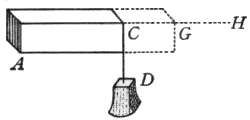
\includegraphics[width=6.25cm,height=3.00cm,keepaspectratio]{images/figura29.png} \end{center}
\end{center}

Sia dato il prisma \emph{AC} col suo proprio peso, e dato parimente il peso \emph{D}, massimo da poter esser sostenuto dall'estremità \emph{C}: bisogna trovare la lunghezza massima sino alla quale si possa allungare il detto prisma senza rompersi. Facciasi, come il peso del prisma \emph{AC} al composto de i pesi \emph{AC} col doppio del peso di \emph{D}, così la lunghezza \emph{CA} alla \emph{AH}, tra le quali sia media proporzionale la \emph{AG}: dico, \emph{AG} esser la lunghezza cercata. Imperò che il momento gravante del peso \emph{D} in \emph{C} è eguale al momento del peso doppio di \emph{D} che fusse posto nel mezo di \emph{AC}, dove è anco il centro del momento del prisma \emph{AC}; il momento dunque della resistenza del prisma \emph{AC}, che sta in \emph{A}, equivale al gravante del doppio del peso \emph{D} col peso \emph{AC}, attaccati però nel mezo di \emph{AC}. E perché viene ad essersi fatto, come 'l momento di detti pesi così situati, cioè del doppio \emph{D} con \emph{AC}, al momento di \emph{AC}, così la \emph{HA} alla \emph{AC}, tra le quali è media la \emph{AG}, adunque il momento del doppio \emph{D} col momento \emph{AC} al momento \emph{AC} è come il quadrato \emph{GA} al quadrato \emph{AC}: ma il momento premente del prisma \emph{GA} al momento di \emph{AC} è come il quadrato \emph{GA} al quadrato \emph{AC}: adunque la lunghezza \emph{AG} è la massima che si cercava, cioè quella sino alla quale allungandosi il prisma \emph{AC} si sosterrebbe, ma più oltre si spezzerebbe.

Sin qui si son considerati i momenti e le resistenze de i prismi e cilindri solidi, l'una estremità de i quali sia posta immobile, e solo nell'altra sia applicata la forza di un peso premente, considerandolo esso solo, o ver congiunto con la gravità del medesimo solido, o veramente la sola gravità dell'istesso solido: ora voglio che discorriamo alquanto de i medesimi prismi e cilindri quando fussero sostenuti da amendue l'estremità, o vero che sopra un sol punto, preso tra le estremità, fusser posati. E prima dico, che il cilindro che gravato dal proprio peso sarà ridotto alla massima lunghezza, oltre alla quale più non si sosterrebbe, o sia retto nel mezo da un solo sostegno o vero da due nelle estremità, potrà esser lungo il doppio di quello che sarebbe, fitto nel muro, cioè sostenuto in un sol termine.


\begin{center}
\begin{center} 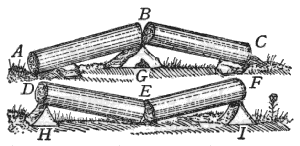
\includegraphics[width=7.50cm,height=3.65cm,keepaspectratio]{images/figura30.png} \end{center}
\end{center}

Il che per se stesso è assai manifesto perché se intenderemo, del cilindro che io segno \emph{ABC}, la sua metà \emph{AB} esser la somma lunghezza potente a sostenersi stando fissa nel termine \emph{B}, nell'istesso modo si sosterrà se, posata sopra 'l sostegno \emph{G}, sarà contrappesata dall'altra sua metà \emph{BC}. E similmente, se del cilindro \emph{DEF} la lunghezza sarà tale, che solamente la sua metà potesse sostenersi fissa nel termine \emph{D}, ed in consequenza l'altra \emph{EF} fissa nel termine \emph{F}, è manifesto che posti i sostegni \emph{H}, \emph{I} sotto l'estremità \emph{D}, \emph{F}, ogni momento che si aggiunga di forza o di peso in \emph{E}, quivi si farà la rottura.

Quello che ricerca più sottile specolazione è quando, astraendo dalla gravità di tali solidi, ci fusse proposto di dovere investigare se quella forza o peso che, applicato al mezo d'un cilindro sostenuto nelle estremità, basterebbe a romperlo, potrebbe far l'istesso effetto applicato in qualsivoglia altro luogo, più vicino all'una che all'altra estremità: come, per esempio, se volendo noi rompere una mazza, presola con le mani nell'estremità ed appuntato il ginocchio in mezo, l'istessa forza che basterebbe usare per romperla in tal modo, basterebbe ancora quando il ginocchio si puntasse non nel mezzo, ma più vicino all'un de gli estremi.

\speaker{Sagr.} Parmi che 'l problema sia toccato da Aristotele nelle sue Questioni Mecaniche.

\speaker{Salv.} Il quesito d'Aristotele non è precisamente l'istesso, perché ei non cerca altro, se non di render la ragione perché manco fatica si ricerchi a romperlo tenendo le mani nell'estremità del legno, cioè remote assai dal ginocchio, che se le tenessimo vicine: e ne rende una ragione generale, riducendo la causa alle leve più lunghe, quando s'allargano le braccia afferrando l'estremità. Il nostro quesito aggiugne qualche cosa di più, ricercando se, posto il ginocchio nel mezo o in altro luogo, tenendo pur le mani sempre nell'estremità, la medesima forza serva in tutti i siti.

\speaker{Sagr.} Nella prima apprensione parrebbe di sì, atteso che le due leve mantengono in certo modo il medesimo momento, mentre che, quanto si scorcia l'una, tanto s'allunga l'altra.

\speaker{Salv.} Or vedete quanto sono in pronto l'equivocazioni, e con quanta cautela e circospezione convien andare per non v'incorrere. Cotesto che voi dite, e che veramente nel primo aspetto ha tanto del verisimile, in ristretto poi è tanto falso, che quando il ginocchio, che è il fulcimento delle due leve, sia posto o non posto nel mezo, fa tal diversità, che di quella forza che basterebbe per far la frazzione nel mezo, dovendola fare in qualche altro luogo, tal volta non basterà l'applicarvene quattro volte tanto, né dieci, né cento, né mille. Faremo sopra ciò una tal quale considerazion generale, e poi verremo alla specifica determinazione della proporzione secondo la quale si vanno variando le forze per far la frazzione più in un punto che in un altro.


\begin{center}
\begin{center} 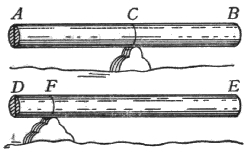
\includegraphics[width=6.25cm,height=3.90cm,keepaspectratio]{images/figura31.png} \end{center}
\end{center}

Segniamo prima questo legno \emph{AB}, da rompersi nel mezo sopra 'l sostegno \emph{C}, ed appresso segniamo l'istesso, ma sotto caratteri \emph{DE}, da rompersi sopra 'l sostegno \emph{F}, remoto dal mezo. Prima, è manifesto che sendo le distanze \emph{AC}, \emph{CB} eguali, la forza sarà compartita egualmente nelle estremità \emph{B}, \emph{A}. Secondo, poi che la distanza \emph{DF} diminuisce dalla distanza \emph{AC}, il momento della forza posta in \emph{D} sciema dal momento in \emph{A}, cioè posto nella distanza \emph{CA}, e sciema secondo la proporzione della linea \emph{DF} alla \emph{AC}, ed in consequenza bisogna crescerlo per pareggiare o superar la resistenza di \emph{F}: ma la distanza \emph{DF} si può diminuire in infinito in relazione alla distanza \emph{AC}: adunque bisogna poter crescere in infinito la forza da applicarsi in \emph{D} per pareggiar la resistenza in \emph{F}. Ma all'incontro, secondo che cresce la distanza \emph{FE} sopra la \emph{CB}, convien diminuire la forza in \emph{E} per pareggiare la resistenza in \emph{F}: ma la distanza \emph{FE} in relazione alla \emph{CB} non si può crescere in infinito col ritirar il sostegno \emph{F} verso il termine \emph{D}, anzi né anco il doppio: adunque la forza in \emph{E} per pareggiare la resistenza in \emph{F} sarà sempre più che la metà della forza in \emph{B}. Comprendesi dunque la necessità del doversi agumentare i momenti del congiunto delle forze in \emph{E}, \emph{D} infinitamente per pareggiare o superar la resistenza posta in \emph{F}, secondo che il sostegno \emph{F} s'andrà approssimando verso l'estremità \emph{D}.

\speaker{Sagr.} Che diremo, Sig. Simplicio? non convien egli confessare, la virtù della geometria esser il più potente strumento d'ogni altro per acuir l'ingegno e disporlo al perfettamente discorrere e specolare? e che con gran ragione voleva Platone i suoi scolari prima ben fondati nelle matematiche? Io benissimo avevo compreso la facultà della leva, e come crescendo o sciemando la sua lunghezza, cresceva o calava il momento della forza e della resistenza; con tutto ciò nella determinazione del presente problema m'ingannavo, e non di poco, ma d'infinito.

\speaker{Simp.} Veramente comincio a comprendere che la logica, benché strumento prestantissimo per regolare il nostro discorso, non arriva, quanto al destar la mente all'invenzione, all'acutezza della geometria.

\speaker{Sagr.} A me pare che la logica insegni a conoscere se i discorsi e le dimostrazioni già fatte e trovate procedano concludentemente; ma che ella insegni a trovare i discorsi e le dimostrazioni concludenti, ciò veramente non credo io. Ma sarà meglio che il Sig. Salviati ci mostri secondo qual proporzione vadian crescendo i momenti delle forze per superar la resistenza del medesimo legno secondo i luoghi diversi della rottura.

\speaker{Salv.} La proporzione, che ricercate, procede in cotal forma, che:


\begin{enunciato}
Se nella lunghezza d'un cilindro si noteranno due luoghi sopra i quali si voglia far la frazzione di esso cilindro, le resistenze di detti due luoghi hanno fra di loro la medesima proporzione che i rettangoli fatti dalle distanze di essi luoghi contrariamente presi.
\end{enunciato}


\begin{center}
\begin{center} 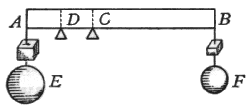
\includegraphics[width=6.25cm,height=2.78cm,keepaspectratio]{images/figura32.png} \end{center}
\end{center}

Siano le forze \emph{A}, \emph{B} minime per rompere in \emph{C}, e le \emph{E}, \emph{F} parimente le minime per rompere in \emph{D}: dico, le forze \emph{A}, \emph{B} alle forze \emph{E}, \emph{F} aver la proporzion medesima che ha il rettangolo \emph{ADB} al rettangolo \emph{ACB}. Imperò che le forze \emph{A}, \emph{B} alle forze \emph{E}, \emph{F} hanno la proporzion composta delle forze \emph{A}, \emph{B} alla forza \emph{B}, della \emph{B} alla \emph{F}, e della \emph{F} alle \emph{F}, \emph{E}: ma come le forze \emph{A}, \emph{B} alla forza \emph{B}, così sta la lunghezza \emph{BA} ad \emph{AC}; e come la forza \emph{B} alla \emph{F}, così sta la linea \emph{DB} alla \emph{BC}; e come la forza \emph{F} alle \emph{F}, \emph{E}, così sta la linea \emph{DA} alla \emph{AB}: adunque le forze \emph{A}, \emph{B} alle forze \emph{E}, \emph{F} hanno la proporzion composta delle tre, cioè della retta \emph{BA} ad \emph{AC}, della \emph{DB} a \emph{BC}, e della \emph{DA} ad \emph{AB}. Ma delle due \emph{DA} ad \emph{AB}, ed \emph{AB} ad \emph{AC}, si compone la proporzione della \emph{DA} ad \emph{AC}; adunque le forze \emph{A}, \emph{B} alle forze \emph{E}, \emph{F} hanno la proporzion composta di questa \emph{DA} ad \emph{AC} e dell'altra \emph{DB} a \emph{BC}. Ma il rettangolo \emph{ADB} al rettangolo \emph{ACB} ha la proporzion composta delle medesime \emph{DA} ad \emph{AC} e \emph{DB} a \emph{BC}: adunque le forze \emph{A}, \emph{B} alle \emph{E}, \emph{F} stanno come il rettangolo \emph{ADB} al rettangolo \emph{ACB}: che è quanto a dire, la resistenza in \emph{C} ad essere spezzato alla resistenza ad esser rotto in \emph{D} aver la medesima proporzione che il rettangolo \emph{ADB} al rettandolo \emph{ACB}: che è quello che si doveva provare.

In consequenza di questo teorema possiamo risolvere un problema assai curioso; ed è:


\begin{enunciato}
Dato il peso massimo retto dal mezo di un cilindro o prisma, dove la resistenza è minima, e dato un peso maggior di quello, trovare nel detto cilindro il punto nel quale il dato peso maggiore sia retto come peso massimo.
\end{enunciato}


\begin{center}
\begin{center} 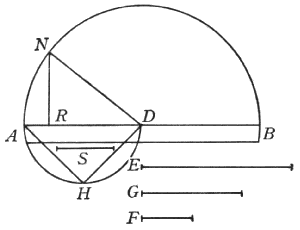
\includegraphics[width=7.50cm,height=5.75cm,keepaspectratio]{images/figura33.png} \end{center}
\end{center}

Abbia il dato peso, maggiore del peso massimo retto dal mezo del cilindro \emph{AB}, ad esso massimo la proporzione della linea \emph{E} alla \emph{F}: bisogna trovare il punto nel cilindro dal quale il dato peso venga sostenuto come massimo. Tra le due \emph{E}, \emph{F} sia media proporzionale la \emph{G}, e come la \emph{E} alla \emph{G}, così si faccia la \emph{AD} alla \emph{S}: sarà la \emph{S} minore della \emph{AD}. Sia \emph{AD} diametro del mezo cerchio \emph{AHD}, nel quale pongasi la \emph{AH} eguale alla \emph{S}, e congiungasi \emph{HD}, e ad essa si tagli eguale la \emph{DR}: dico, il punto \emph{R} essere il cercato, dal quale il dato peso, maggiore del massimo retto dal mezo del cilindro \emph{D}, verrebbe come massimo retto. Sopra la lunghezza \emph{BA} facciasi il mezo cerchio \emph{ANB}, e si alzi la perpendicolare \emph{RN}, e congiungasi \emph{ND}: e perché i due quadrati \emph{NR}, \emph{RD} sono eguali al quadrato \emph{ND}, cioè al quadrato \emph{AD}, cioè alli due \emph{AH}, \emph{HD}, e l'\emph{HD} è eguale al quadrato \emph{DR}, adunque il quadrato \emph{NR}, cioè il rettangolo \emph{ARB}, sarà eguale al quadrato \emph{AH}, cioè al quadrato \emph{S}; ma il quadrato \emph{S} al quadrato \emph{AD} è come la \emph{F} alla \emph{E}, cioè come il peso massimo retto in \emph{D} al dato peso maggiore; adunque questo maggiore sarà retto in \emph{R} come il massimo che vi possa esser sostenuto: che è quello che si cercava.

\speaker{Sagr.} Intendo benissimo: e vo considerando che, essendo il prisma \emph{AB} sempre più gagliardo e resistente alla pressione nelle parti che più e più si allontanano dal mezo, nelle travi grandissime e gravi se ne potrebbe levar non piccola parte verso l'estremità, con notabile alleggerimento di peso, che ne i travamenti di grandi stanze sarebbe di commodo ed utile non piccolo. E bella cosa sarebbe il ritrovar quale figura devrebbe aver quel tal solido che in tutte le sue parti fusse egualmente resistente, tal che non più facile fusse ad esser rotto da un peso che lo premesse nel mezo, che in qualsivoglia altro luogo.

\speaker{Salv.} Già ero in procinto di dirvi cosa assai notabile e vaga in questo proposito. Fo un poco di figura per meglio dichiararmi.


\begin{center}
\begin{center} 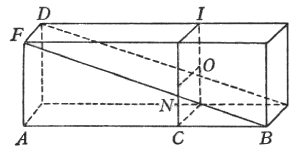
\includegraphics[width=7.50cm,height=3.80cm,keepaspectratio]{images/figura34.png} \end{center}
\end{center}

Questo \emph{DB} è un prisma, la cui resistenza ad essere spezzato nell'estremità \emph{AD} da una forza premente nel termine \emph{B} è tanto minore della resistenza che si troverebbe nel luogo \emph{CI}, quanto la lunghezza \emph{CB} è minore della \emph{BA}, come già si è dimostrato. Intendasi adesso il medesimo prisma segato diagonalmente secondo la linea \emph{FB}, sì che le faccie opposte siano due triangoli, uno de i quali, verso noi, è questo \emph{FAB}: ottiene tal solido contraria natura del prisma, cioè che meno resiste all'essere spezzato sopra 'l termine \emph{C} che sopra l'\emph{A} dalla forza posta in \emph{B}, quanto la lunghezza \emph{CB} è minore della \emph{BA}. Il che facilmente proveremo: perché intendendo il taglio \emph{CNO} parallelo all'altro \emph{AFD}, la linea \emph{FA} alla \emph{CN} nel triangolo \emph{FAB} arà la medesima proporzione che la linea \emph{AB} alla \emph{BC}; e però se noi intenderemo, ne i punti \emph{A}, \emph{C} esser i sostegni di due leve, le cui distanze \emph{BA}, \emph{AF}, \emph{BC}, \emph{CN}, queste saranno simili; e però quel momento che ha la forza posta in \emph{B} con la distanza \emph{BA} sopra la resistenza posta nella distanza \emph{AF}, l'arà la medesima forza in \emph{B} con la distanza \emph{BC} sopra la medesima resistenza che fusse posta nella distanza \emph{CN}: ma la resistenza da superarsi nel sostegno \emph{C}, posta nella distanza \emph{CN}, dalla forza in \emph{B}, è minore della resistenza in \emph{A} tanto, quanto il rettangolo \emph{CO} è minore del rettangolo \emph{AD}, cioè quanto la linea \emph{CN} è minore della \emph{AF}, cioè la \emph{CB} della \emph{BA}: adunque la resistenza della parte \emph{OCB} ad esser rotto in \emph{C} è tanto minore della resistenza dell'intero \emph{DAB} ad esser rotto in \emph{A}, quanto la lunghezza \emph{CB} è minore della \emph{AB}. Aviamo dunque nel trave o prisma \emph{DB} levatone una parte, cioè la metà, segandolo diagonalmente, e lasciato il cuneo o prisma triangolare \emph{FBA}; e sono due solidi di condizioni contrarie, cioè quello tanto più resiste quanto più si scorcia, e questo nello scorciarsi perde altrettanto di robustezza. Ora, stante questo, par ben ragionevole, anzi pur necessario, che se gli possa dare un taglio, per il quale, togliendo via il superfluo, rimanga un solido di figura tale, che in tutte le sue parti sia egualmente resistente.

\speaker{Simp.} È ben necessario che dove si passa dal maggiore al minore, s'incontri ancora l'eguale.

\speaker{Sagr.} Ma il punto sta ora a trovar come si ha guidar la sega per far questo taglio.

\speaker{Simp.} Questo mi si rappresenta che dovrebbe esser opera assai facile; perché, se col segar il prisma diagonalmente, levandone la metà, la figura che resta ritien contraria natura a quella del prisma intero, sì che in tutti i luoghi ne i quali questo acquistava robustezza, quello altrettanto la perdeva, parmi che tenendo la via del mezo, cioè levando solamente la metà di quella metà, che è la quarta parte del tutto, la rimanente figura non guadagnerà né perderà robustezza in tutti quei medesimi luoghi ne i quali la perdita e il guadagno dell'altre due figure erano sempre eguali.

\speaker{Salv.} Voi, Sig. Simplicio, non avete dato nel segno: e sì come io vi mostrerò, vedrete veramente che quello che si può segar del prisma e levar via senza indebolirlo, non è la sua quarta parte, ma la terza. Ora resta (che è quello che accennava il Sig. Sagredo) il ritrovar secondo che linea si deve far camminar la sega: la quale proverò che deve esser linea parabolica. Ma prima è necessario dimostrare certo lemma, che è tale:


\begin{enunciato}
Se saranno due libre o leve, divise da i loro sostegni in modo, che le due distanze dove si hanno a costituire le potenze, abbiano tra di loro doppia proporzione delle distanze dove saranno le resistenze, le quali resistenze siano tra loro come le lor distanze, le potenze sostenenti saranno eguali.
\end{enunciato}


\begin{center}
\begin{center} 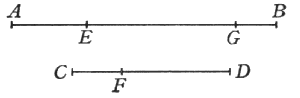
\includegraphics[width=7.50cm,height=2.45cm,keepaspectratio]{images/figura35.png} \end{center}
\end{center}

Siano due leve \emph{AB}, \emph{CD}, divise sopra i lor sostegni \emph{E}, \emph{F} talmente, che la distanza \emph{EB} alla \emph{FD} abbia doppia proporzione di quella che ha la distanza \emph{EA} alla \emph{FC}; ed intendansi in \emph{A}, \emph{C} resistenze tra di loro nella proporzione di \emph{EA}, \emph{FC}: dico, le potenze che in \emph{B}, \emph{D} sosterranno le resistenze di \emph{A}, \emph{C} esser tra loro eguali. Pongasi la \emph{EG} media proporzionale tra \emph{EB} e \emph{FD}: sarà dunque come \emph{BE} ed \emph{EG}, così \emph{GE} ad \emph{FD} ed \emph{AE} a \emph{CF}; e così si è posto esser la resistenza di \emph{A} alla resistenza di \emph{C}. E perché come \emph{EG} ad \emph{FD}, così \emph{AE} a \emph{CF}, sarà, permutando, come \emph{GE} ad \emph{EA} così \emph{DF} ad \emph{FC}; e però (per esser le due leve \emph{DC}, \emph{GA} divise proporzionalmente ne i punti \emph{F}, \emph{E}) quando la potenza che posta in \emph{D} pareggia la resistenza di \emph{C}, fusse in \emph{G}, pareggerebbe la medesima resistenza di \emph{C} posta in \emph{A}: ma, per il dato, la resistenza di \emph{C} ha la medesima proporzione che la \emph{AE} alla \emph{CF}, cioè che la \emph{BE} alla \emph{EG}: adunque la potenza \emph{G}, o vogliam dire \emph{D}, posta in \emph{B}, sosterrà la resistenza posta in \emph{A}: che è quello che si doveva provare.


\begin{center}
\begin{center} 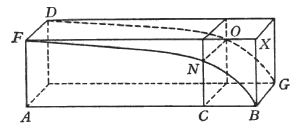
\includegraphics[width=7.50cm,height=3.28cm,keepaspectratio]{images/figura36.png} \end{center}
\end{center}

Inteso questo, nella faccia \emph{FB} del prisma \emph{DB} sia segnata la linea parabolica \emph{FNB}, il cui vertice \emph{B}, secondo la quale sia segato esso prisma, restando il solido compreso dalla base \emph{AD}, dal piano rettangolo \emph{AG}, dalla linea retta \emph{BG} e dalla superficie \emph{DGBF}, incurvata secondo la curvità della linea parabolica \emph{FNB}: dico, tal solido esser per tutto egualmente resistente. Sia segato dal piano \emph{CO}, parallelo all'\emph{AD}, e intendansi due leve divise e posate sopra i sostegni \emph{A}, \emph{C}, e siano dell'una le distanze \emph{BA}, \emph{AF}, e dell'altra le \emph{BC}, \emph{CN}. E perché nella parabola \emph{FBA} la \emph{AB} alla \emph{BC} sta come il quadrato della \emph{FA} al quadrato di \emph{CN}, è manifesto, la distanza \emph{BA} dell'una leva alla distanza \emph{BC} dell'altra aver doppia proporzione di quella che ha l'altra distanza \emph{AF} all'altra \emph{CN}: e perché la resistenza da pareggiarsi con la leva \emph{BA} alla resistenza da pareggiarsi con la leva \emph{BC} ha la medesima proporzione che 'l rettangolo \emph{DA} al rettangolo \emph{OC}, la quale è la medesima che ha la linea \emph{AF} alla \emph{NC}, che sono l'altre due distanze delle leve, è manifesto, per il lemma passato, che la medesima forza che sendo applicata alla linea \emph{BG} pareggerà la resistenza \emph{DA}, pareggerà ancora la resistenza \emph{CO}. Ed il medesimo si dimostrerà segandosi il solido in qual si sia altro luogo: adunque tal solido parabolico è per tutto egualmente resistente. Che poi, segandosi il prisma secondo la linea parabolica \emph{FNB}, se ne levi la terza parte, si fa manifesto: perché la semiparabola \emph{FNBA} e 'l rettangolo \emph{FB} son basi di due solidi compresi tra due piani paralleli, cioè tra i rettangoli \emph{FB}, \emph{DG}, per lo che ritengono tra di loro la medesima proporzione che esse lor basi; ma il rettangolo \emph{FB} è sesquialtero della semiparabola \emph{FNBA}; adunque, segando il prisma secondo la linea parabolica, se ne leva la terza parte. Di qui si vede come con diminuzion di peso di più di trentatré per cento si posson far i travamenti, senza diminuir punto la loro gagliardia; il che ne i navilii grandi, in particolare per regger le coverte, può esser d'utile non piccolo, atteso che in cotali fabbriche la leggerezza importa infinitamente.

\speaker{Sagr.} Le utilità son tante, che lungo o impossibil sarebbe il registrarle tutte: ma io, lasciate queste da banda, arei più gusto d'intender che l'alleggerimento si faccia secondo le proporzioni assegnate. Che il taglio secondo la diagonale levi la metà del peso, l'intendo benissimo; ma che l'altro, secondo la parabolica, porti via la terza parte del prisma, posso crederlo al Sig. Salviati, sempre veridico, ma in ciò più della fede mi sarebbe grata la scienza.

\speaker{Salv.} Vorreste dunque aver la dimostrazione, come sia vero che l'eccesso del prisma sopra questo che per ora chiamiamo solido parabolico, sia la terza parte di tutto il prisma. So d'averlo altra volta dimostrato; tenterò ora se potrò rimetter insieme la dimostrazione, per la quale intanto mi sovvien che mi servivo di certo lemma d'Archimede, posto da esso nel libro delle Spirali: ed è, che se quante linee si vogliono si eccederanno egualmente, e l'eccesso sia eguale alla minima di quelle, ed altrettante siano ciascheduna eguale alla massima, i quadrati di tutte queste saranno meno che tripli de i quadrati di quelle che si eccedono; ma i medesimi saranno ben più che tripli di quelli altri che restano, trattone il quadrato della massima.


\begin{center}
\begin{center} 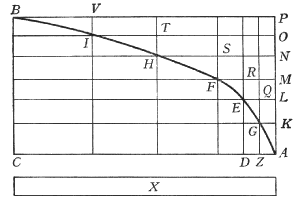
\includegraphics[width=7.50cm,height=5.10cm,keepaspectratio]{images/figura37.png} \end{center}
\end{center}

Posto questo, sia in questo rettangolo \emph{ACBP} inscritta la linea parabolica \emph{AB}: doviamo provare, il triangolo misto \emph{BAP}, i cui lati sono \emph{BP}, \emph{PA} e base la linea parabolica \emph{BA}, esser la terza parte di tutto 'l rettangolo \emph{CP}. Imperò che, se non è tale, sarà o più che la terza parte o meno. Sia, se esser può, meno, ed a quello che gli manca intendasi esser eguale lo spazio \emph{X}. Dividendo poi il rettangolo \emph{CP} continuamente in parti eguali con linee parallele a i lati \emph{BP}, \emph{CA} arriveremo finalmente a parti tali, ch'una di loro sarà minore dello spazio \emph{X}: or sia una di quelle il rettangolo \emph{OB}, e per i punti dove l'altre parallele segano la linea parabolica, facciansi passare le parallele alla \emph{AP}; e qui intenderò circoscritta intorno al nostro triangolo misto una figura composta di rettangoli, che sono \emph{BO}, \emph{IN}, \emph{HM}, \emph{FL}, \emph{EK}, \emph{GA}, la qual figura sarà pur ancora meno che la terza parte del rettangolo \emph{CP}, essendo che l'eccesso di essa figura sopra 'l triangolo misto è manco assai del rettangolo \emph{BO}, il quale è ancor minore dello spazio \emph{X}.

\speaker{Sagr.} Piano, di grazia, ch'io non vedo come l'eccesso di questa figura circoscritta sopra 'l triangolo misto sia manco assai del rettangolo \emph{BO}.

\speaker{Salv.} Il rettangolo \emph{BO} non è egli eguale a tutti questi rettangoletti per i quali passa la nostra linea parabolica? dico di questi \emph{BI}, \emph{IH}, \emph{HF}, \emph{FE}, \emph{EG}, \emph{GA}, de i quali una parte sola resta fuori del triangolo misto? ed il rettangolo \emph{BO} non si è egli posto ancor minore nello spazio \emph{X}? Adunque, se il triangolo insieme con l'\emph{X} pareggiava, per l'avversario, la terza parte del rettangolo \emph{CP}, la figura circoscritta, che al triangolo aggiugne tanto meno che lo spazio \emph{X}, resterà pur ancora minore della terza parte del rettangolo medesimo \emph{CP}: ma questo non può essere, perché ella è più della terza parte: adunque non è vero che il nostro triangolo misto sia manco del terzo del rettangolo.

\speaker{Sagr.} Ho intesa la soluzione del mio dubbio. Ma bisogna ora provarci che la figura circoscritta sia più della terza parte del rettangolo \emph{CP}, dove credo che aremo assai più da fare.

\speaker{Salv.} Eh non ci è gran difficoltà. Imperò che nella parabola il quadrato della linea \emph{DE} al quadrato della \emph{ZG} ha la medesima proporzione che la linea \emph{DA} alla \emph{AZ}, che è quella che ha il rettangolo \emph{KE} al rettangolo \emph{AG} (per esser l'altezze \emph{AK}, \emph{KL} eguali); adunque la proporzione che ha il quadrato \emph{ED} al quadrato \emph{ZG}, cioè il quadrato \emph{LA} al quadrato \emph{AK}, l'ha ancora il rettangolo \emph{KE} al rettangolo \emph{KZ}. E nel medesimo modo appunto si proverà de gli altri rettangoli \emph{LF}, \emph{MH}, \emph{NI}, \emph{OB} star tra di loro come i quadrati delle linee \emph{MA}, \emph{NA}, \emph{OA}, \emph{PA}. Consideriamo adesso come la figura circoscritta è composta di alcuni spazii che tra di loro stanno come i quadrati di linee che si eccedono con eccessi eguali alla minima, e come il rettangolo \emph{CP} è composto di altrettanti spazii ciascuno eguale al massimo, che sono tutti i rettangoli eguali all'\emph{OB}; adunque, per il lemma d'Archimede, la figura circoscritta è più della terza parte del rettangolo \emph{CP}: ma era anche minore, il che è impossibile: adunque il triangolo misto non è manco del terzo del rettangolo \emph{CP}. Dico parimente che non è più. Imperò che, se è più del terzo del rettangolo \emph{CP}, intendasi lo spazio \emph{X} eguale all'eccesso del triangolo sopra la terza parte di esso rettangolo \emph{CP}; e fatta la divisione e suddivisione del rettangolo in rettangoli sempre eguali, si arriverà a tale che uno di quelli sia minore dello spazio \emph{X}. Sia fatta, e sia il rettangolo \emph{BO} minore dell'\emph{X}; e descritta come sopra la figura, avremo nel triangolo misto inscritta una figura composta de i rettangoli \emph{VO}, \emph{TN}, \emph{SM}, \emph{RL}, \emph{QK}, la quale non sarà ancora minore della terza parte del gran rettangolo \emph{CP}. Imperò che il triangolo misto supera di manco assai la figura inscritta di quello che egli superi la terza parte di esso rettangolo \emph{CP}, atteso che l'eccesso del triangolo sopra la terza parte del rettangolo \emph{CP} è eguale allo spazio \emph{X}, il quale è minore del rettangolo \emph{BO}, e questo è anco minore assai dell'eccesso del triangolo sopra la figura inscrittagli; imperò che ad esso rettangolo \emph{BO} sono eguali tutti i rettangoletti \emph{AG}, \emph{GE}, \emph{EF}, \emph{FH}, \emph{HI}, \emph{IB}, de i quali son ancora manco che la metà gli avanzi del triangolo sopra la figura inscritta. E però, avanzando il triangolo la terza parte del rettangolo \emph{CP} di più assai (avanzandolo dello spazio \emph{X}) che ei non avanza la sua figura inscritta, sarà tal figura ancora maggiore della terza parte del rettangolo \emph{CP}: ma ella è minore, per il lemma supposto; imperò che il rettangolo \emph{CP}, come aggregato di tutti i rettangoli massimi, a i rettangoli componenti la figura inscritta ha la medesima proporzione che l'aggregato di tutti i quadrati delle linee eguali alla massima a i quadrati delle linee che si eccedono egualmente, trattone il quadrato della massima; e però (come de i quadrati accade) tutto l'aggregato de i massimi (che è il rettangolo \emph{CP}) è più che triplo dell'aggregato de gli eccedentisi, trattone il massimo, che compongono la figura inscritta. Adunque il triangolo misto non è né maggiore né minore della terza parte del rettangolo \emph{CP}; è dunque eguale.

\speaker{Sagr.} Bella e ingegnosa dimostrazione, e tanto più, quanto ella ci dà la quadratura della parabola, mostrandola essere sesquiterza del triangolo inscrittogli, provando quello che Archimede con due tra di loro diversissimi, ma amendue ammirabili, progressi di molte proposizioni dimostrò; come anco fu dimostrata ultimamente da Luca Valerio, altro Archimede secondo dell'età nostra, la qual dimostrazione è registrata nel libro che egli scrisse del centro della gravità de i solidi.

\speaker{Salv.} Libro veramente da non esser posposto a qual si sia scritto da i più famosi geometri del presente e di tutti i secoli passati; il quale quando fu veduto dall'Accademico nostro, lo fece desistere dal proseguire i suoi trovati, che egli andava continuando di scrivere sopra 'l medesimo suggetto, già che vedde il tutto tanto felicemente ritrovato e dimostrato dal detto Sig. Valerio.

\speaker{Sagr.} Io ero informato di tutto questo accidente dall'istesso Accademico: e l'avevo anco ricercato che mi lasciasse una volta vedere le sue dimostrazioni sin allora ritrovate quando ei s'incontrò nel libro del Sig. Valerio, ma non mi successe poi il vederle.

\speaker{Salv.} Io ne ho copia, e le mostrerò a V. S., che averà gusto di vedere la diversità de i metodi con i quali camminano questi due autori per l'investigazione delle medesime conclusioni e loro dimostrazioni; dove anco alcune delle conclusioni hanno differente esplicazione, benché in effetto egualmente vere.

\speaker{Sagr.} Mi sarà molto caro il vederle, e V. S., quando ritorni a i soliti congressi, mi farà grazia di portarle seco. Ma intanto, essendo questa, della resistenza del solido cavato dal prisma col taglio parabolico, operazione non men bella che utile in molte opere mecaniche, buona cosa sarebbe per gli artefici l'aver qualche regola facile e spedita per potere sopra 'l piano del prisma segnare essa linea parabolica.

\speaker{Salv.} Modi di disegnar tali linee ce ne son molti, ma due sopra tutti gli altri speditissimi glie ne dirò io: uno de i quali è veramente maraviglioso, poiché con esso, in manco tempo che col compasso altri disegnerà sottilmente sopra una carta quattro o sei cerchi di differenti grandezze, io posso disegnare trenta e quaranta linee paraboliche, non men giuste sottili e pulite delle circonferenze di essi cerchi. Io ho una palla di bronzo esquisitamente rotonda, non più grande d'una noce; questa, tirata sopra uno specchio di metallo, tenuto non eretto all'orizonte, ma alquanto inchinato, sì che la palla nel moto vi possa camminar sopra, calcandolo leggiermente nel muoversi, lascia una linea parabolica sottilissimamente e pulitissimamente descritta, e più larga e più stretta secondo che la proiezzione si sarà più o meno elevata. Dove anco abbiamo chiara e sensata esperienza, il moto de i proietti farsi per linee paraboliche: effetto non osservato prima che dal nostro amico, il quale ne arreca anco la dimostrazione nel suo libro del moto, che vedremo insieme nel primo congresso. La palla poi, per descrivere al modo detto le parabole, bisogna, con maneggiarla alquanto con la mano, scaldarla ed alquanto inumidirla, ché così lascerà più apparenti sopra lo specchio i suoi vestigii. L'altro modo, per disegnar la linea, che cerchiamo, sopra il prisma, procede così. Ferminsi ad alto due chiodi in un parete, equidistanti all'orizonte e tra di loro lontani il doppio della larghezza del rettangolo su 'l quale vogliamo notare la semiparabola, e da questi due chiodi penda una catenella sottile, e tanto lunga che la sua sacca si stenda quanta è la lunghezza del prisma: questa catenella si piega in figura parabolica, sì che andando punteggiando sopra 'l muro la strada che vi fa essa catenella, aremo descritta un'intera parabola, la quale con un perpendicolo, che penda dal mezo di quei due chiodi, si dividerà in parti eguali. Il trasferir poi tal linea sopra le faccie opposte del prisma non ha difficoltà nessuna, sì che ogni mediocre artefice lo saprà fare. Potrebbesi anco con l'aiuto delle linee geometriche segnate su 'l compasso del nostro amico, senz'altra fattura, andar su l'istessa faccia del prisma punteggiando la linea medesima.

Abbiamo sin qui dimostrate tante conclusioni attenenti alla contemplazione di queste resistenze de i solidi all'essere spezzati, con l'aver prima aperto l'ingresso a tale scienza col suppor come nota la resistenza per diritto, che si potrà consequentemente camminar avanti, ritrovandone altre ed altre conclusioni, e loro dimostrazioni, di quelle che in natura sono infinite. Solo per ora, per ultimo termine de gli odierni ragionamenti, voglio aggiugnere la specolazione delle resistenze de i solidi vacui, de i quali l'arte, e più la natura, si serve in mille operazioni, dove senza crescer peso si cresce grandemente la robustezza, come si vede nell'ossa de gli uccelli ed in moltissime canne, che son leggiere e molto resistenti al piegarsi e rompersi: che se un fil di paglia, che sostien una spiga più grave di tutto 'l gambo, fusse fatto della medesima quantità di materia, ma fusse massiccio, sarebbe assai meno resistente al piegarsi ed al rompersi. E con tal ragione ha osservato l'arte, e confermato l'esperienza, che un'asta vota o una canna di legno o di metallo è molto più salda che se fusse, d'altrettanto peso e della medesima lunghezza, massiccia, che in consequenza sarebbe più sottile; e però l'arte ha trovato di far vote dentro le lancie, quando si desideri averle gagliarde e leggiere. Mostreremo per tanto, come:


\begin{enunciato}
Le resistenze di due cilindri eguali ed egualmente lunghi, l'uno de i quali sia voto e l'altro massiccio, hanno tra di loro la medesima proporzione che i lor diametri.
\end{enunciato}


\begin{center}
\begin{center} 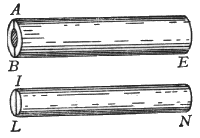
\includegraphics[width=5.00cm,height=3.45cm,keepaspectratio]{images/figura38.png} \end{center}
\end{center}

Siano, la canna o cilindro voto \emph{AE}, ed il cilindro \emph{IN} massiccio, eguali in peso ed egualmente lunghi: dico, la resistenza della canna \emph{AE} all'esser rotta alla resistenza del cilindro solido \emph{IN} aver la medesima proporzione che 'l diametro \emph{AB} al diametro \emph{IL}. Il che è assai manifesto: perché, essendo la canna e 'l cilindro \emph{IN} eguali ed egualmente lunghi, il cerchio \emph{IL}, base del cilindro, sarà eguale alla ciambella \emph{AB}, base della canna \emph{AE} (chiamo \emph{ciambella} la superficie che resta, tratto un cerchio minore dal suo concentrico maggiore), e però le loro resistenze assolute saranno eguali: ma perché nel romper in traverso ci serviamo, nel cilindro \emph{IN}, della lunghezza \emph{LN} per leva, e per sostegno del punto \emph{L}, e del semidiametro o diametro \emph{LI} per contralleva, e nella canna la parte della leva, cioè la linea \emph{BE}, è eguale alla \emph{LN}, ma la contralleva oltre al sostegno \emph{B} è il semidiametro o diametro \emph{AB}, resta manifesto, la resistenza della canna superar quella del cilindro solido secondo l'eccesso del diametro \emph{AB} sopra 'l diametro \emph{IL}: che è quello che cercavamo. S'acquista, dunque, di robustezza nella canna vota sopra la robustezza del cilindro solido secondo la proporzione de i diametri, tutta volta però che amendue siano dell'istessa materia, peso e lunghezza. Sarà bene che conseguentemente andiamo investigando quello che accaggia negli altri casi indifferentemente tra tutte le canne e cilindri solidi egualmente lunghi, benché in quantità di peso diseguali e più e meno evacuati. E prima dimostreremo, come:


\begin{enunciato}
Data una canna vota, si possa trovare un cilindro pieno, eguale ad essa.
\end{enunciato}


\begin{center}
\begin{center} 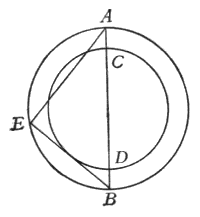
\includegraphics[width=5.00cm,height=5.43cm,keepaspectratio]{images/figura39.png} \end{center}
\end{center}

Facilissima è tal operazione. Imperò che sia la linea \emph{AB} diametro della canna, e \emph{CD} diametro del voto: applichisi nel cerchio maggiore la linea \emph{AE} egual al diametro \emph{CD}, e congiungasi la \emph{EB}. E perché nel mezo cerchio \emph{AEB} l'angolo \emph{E} è retto, il cerchio il cui diametro è \emph{AB}, sarà eguale alli due cerchi de i diametri \emph{AE}, \emph{EB}; ma \emph{AE} è il diametro del voto della canna; adunque il cerchio il cui diametro sia \emph{EB}, sarà egual alla ciambella \emph{ACBD}: e però il cilindro solido, il cerchio della cui base abbia il diametro \emph{EB}, sarà eguale alla canna, essendo egualmente lungo. Dimostrato questo, potremo speditamente


\begin{enunciato}
Trovare qual proporzione abbiano le resistenze d'una canna e di un cilindro, qualunque siano, pur che egualmente lunghi.
\end{enunciato}


\begin{center}
\begin{center} 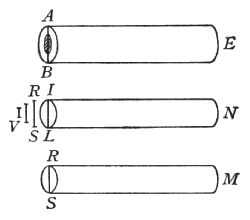
\includegraphics[width=6.25cm,height=5.50cm,keepaspectratio]{images/figura40.png} \end{center}
\end{center}

Sia la canna \emph{ABE}, ed il cilindro \emph{RSM} egualmente lungo: bisogna trovare qual proporzione abbiano tra di loro le lor resistenze. Trovisi, per la precedente, il cilindro \emph{ILN} eguale alla canna ed egualmente lungo, e delle linee \emph{IL}, \emph{RS} (diametri delle basi de i cilindri \emph{IN}, \emph{RM}) sia quarta proporzionale la linea \emph{V}: dico, la resistenza della canna \emph{AE} a quella del cilindro \emph{RM} esser come la linea \emph{AB} alla \emph{V}. Imperò che, essendo la canna \emph{AE} eguale ed egualmente lunga al cilindro \emph{IN}, la resistenza della canna alla resistenza del cilindro starà come la linea \emph{AB} alla \emph{IL}: ma la resistenza del cilindro \emph{IN} alla resistenza del cilindro \emph{RM} sta come il cubo \emph{IL} al cubo \emph{RS}, cioè come la linea \emph{IL} alla \emph{V}; adunque, \emph{ex æquali}, la resistenza della canna \emph{AE} alla resistenza del cilindro \emph{RM} ha la medesima proporzione che la linea \emph{AB} alla \emph{V}: che è quello che si cercava.


\vspace{1.5em}\begin{center}\large\itshape Finisce la seconda Giornata\end{center}

\chapter*{Giornata Terza\\{\normalsize\itshape Del Moto Locale}}
\addcontentsline{toc}{chapter}{Giornata Terza — Del Moto Locale}
\markboth{Giornata Terza}{Del Moto Locale}
Diamo avvio a una nuovissima scienza intorno a un soggetto antichissimo. Nulla v'è, forse, in natura, di più antico del moto, e su di esso ci sono non pochi volumi, né di piccola mole, scritti dai filosofi; tuttavia tra le sue proprietà ne trova molte che, pur degne di essere conosciute, non sono mai state finora osservate, nonché dimostrate. Se ne rilevano alcune più immediate, come quella, ad esempio, che il moto naturale dei gravi discendenti accelera continuamente; però, secondo quale proporzione tale accelerazione avvenga, non è stato sin qui mostrato: nessuno, che io sappia, infatti, ha dimostrato che un mobile discendente a partire dalla quiete percorre, in tempi eguali, spazi che ritengono tra di loro la medesima proporzione che hanno i numeri impari successivi ab unitate. È stato osservato che i corpi lanciati, ovverossia i proietti, descrivono una linea curva di un qualche tipo; però, che essa sia una parabola, nessuno l'ha mostrato. Che sia così, lo dimostrerò insieme ad altre non poche cose, né meno degne di essere conosciute, e, ciò che ritengo ancor più importante, si apriranno le porte a una vastissima e importantissima scienza, della quale queste nostre ricerche costituiranno gli elementi; altri ingegni più acuti del mio ne penetreranno poi più ascosi recessi.

Dividiamo in tre parti la trattazione: nella prima parte consideriamo ciò che concerne il moto equabile o uniforme; nella seconda trattiamo del moto naturalmente accelerato; nella terza, del moto violento, ossia dei proietti.


\section*{DEL MOTO EQUABILE}
\addcontentsline{toc}{section}{Del Moto Equabile}

Circa il moto equabile o uniforme, ci occorre una sola definizione, che formulo così:

\textbf{DEFINIZIONE\\}Moto eguale o uniforme intendo quello in cui gli spazi percorsi da un mobile in tempi eguali, comunque presi, risultano tra di loro eguali.

\textbf{AVVERTENZA\\}Ci è parso opportuno aggiungere alla vecchia definizione (che semplicemente parla di moto equabile, allorché in tempi eguali vengono percorsi spazi eguali) l'espressione comunque presi, cioè per tutti i tempi che siano eguali: infatti, può accadere che in determinati tempi eguali un mobile percorra spazi eguali, mentre spazi, percorsi in frazioni di tempo minori, sebbene eguali, non siano eguali. Dalla precedente definizione dipendono quattro assiomi, cioè:

\textbf{ASSIOMA 1\\}In uno stesso moto equabile, lo spazio percorso in un tempo più lungo è maggiore dello spazio percorso in un tempo più breve.

\textbf{ASSIOMA 2}\\ In uno stesso moto equabile, il tempo in cui è percorso uno spazio maggiore è più lungo del tempo impiegato a percorrere uno spazio minore.

\textbf{ASSIOMA 3}\\ Lo spazio, percorso in un dato tempo a velocità maggiore, è maggiore di quello percorso, nello stesso tempo, a velocità minore.

\textbf{ASSIOMA 4}\\ La velocità, con cui in un dato tempo viene percorso uno spazio maggiore, è maggiore di quella con cui, nello stesso tempo, viene percorso uno spazio minore.

\textbf{TEOREMA 1. PROPOSIZIONE 1}\\ Se un mobile, dotato di moto equabile, percorre due spazi con una stessa velocità, i tempi dei moti staranno tra di loro come gli spazi percorsi.

\textbf{TEOREMA 2. PROPOSIZIONE 2}\\ Se un mobile percorre due spazi in tempi eguali, quegli spazi staranno tra loro come le velocità. E se gli spazi stanno tra loro come le velocità, i tempi saranno eguali.

\textbf{TEOREMA 3. PROPOSIZIONE 3}\\ Se il medesimo spazio viene percorso con velocità diseguali, i tempi dei moti rispondono contrariamente [\emph{sono inversamente proporzionali}] alle velocità.

\textbf{TEOREMA 4. PROPOSIZIONE 4}\\ Se due mobili si muovono di moto equabile, ma con diseguale velocità, gli spazi percorsi da essi in tempi diseguali avranno tra di loro una proporzione composta della proporzione tra le velocità e della proporzione tra i tempi.

\textbf{TEOREMA 5. PROPOSIZIONE 5}\\ Se due mobili si muovono di moto equabile, ma le loro velocità sono diseguali e diseguali gli spazi percorsi, la proporzione tra i tempi risulterà composta della proporzione tra gli spazi e della proporzione tra le velocità permutatamente prese [\emph{proporzione inversa delle velocità}].

\textbf{TEOREMA 6. PROPOSIZIONE 6}\\ Se due mobili si muovono di moto equabile, la proporzione tra le loro velocità risulterà composta della proporzione tra gli spazi percorsi e della proporzione tra i tempi permutatamente presi [\emph{proporzione inversa dei tempi}].

\speaker{Salv.} Questo che abbiamo veduto, è quanto il nostro Autore ha scritto del moto equabile. Passeremo dunque a più sottile e nuova contemplazione intorno al moto naturalmente accelerato, quale è quello che generalmente è esercitato da i mobili gravi descendenti: ed ecco il titolo e l'introduzione.


\section*{DEL MOTO NATURALMENTE ACCELERATO}
\addcontentsline{toc}{section}{Del Moto Naturalmente Accelerato}

Le proprietà del moto equabile sono state considerate nel libro precedente: ora dobbiamo trattare del moto accelerato.

E in primo luogo conviene investigare e spiegare la definizione che corrisponde esattamente al moto accelerato di cui si serve la natura. Infatti, sebbene sia lecito immaginare arbitrariamente qualche forma di moto e contemplare le proprietà che ne conseguono (così, infatti, coloro che si immaginarono linee spirali o concoidi, originate da certi movimenti, ne hanno lodevolmente dimostrate le proprietà argomentando ex suppositione, anche se di tali movimenti non usi la natura), tuttavia, dal momento che la natura si serve di una certa forma di accelerazione nei gravi discendenti, abbiamo stabilito di studiarne le proprietà, posto che la definizione che daremo del nostro moto accelerato abbia a corrispondere con l'essenza del moto naturalmente accelerato. Questa coincidenza crediamo di averla raggiunta finalmente, dopo lunghe riflessioni; soprattutto per il fatto che le proprietà, da noi successivamente dimostrate [dalla nostra definizione], sembrano esattamente corrispondere e coincidere con ciò che gli esperimenti naturali presentano ai sensi. Infine a studiare il moto naturalmente accelerato siamo stati condotti quasi per mano dall'osservazione della consuetudine e della regola seguite dalla natura medesima in tutte le altre sue opere, nella cui attuazione suole far uso dei mezzi più immediati, più semplici, più facili. Ritengo infatti che non vi sia nessuno, il quale creda che si possa praticare il nuoto o il volo in una maniera più semplice e più facile di quella usata, per istinto naturale, dai pesci e dagli uccelli.

Quando, dunque, osservo che una pietra, che discende dall'alto a partire dalla quiete, acquista via via nuovi incrementi di velocità, perché non dovrei credere che tali aumenti avvengano secondo la più semplice e più ovvia proporzione? Ora, se consideriamo attentamente la cosa, non troveremo nessun aumento o incremento più semplice di quello che aumenta sempre nel medesimo modo. Il che facilmente intenderemo considerando la stretta connessione tra tempo e moto: come infatti la equabilità e uniformità del moto si definisce e si concepisce sulla base della eguaglianza dei tempi e degli spazi (infatti chiamiamo equabile il moto, allorché in tempi eguali vengono percorsi spazi eguali), così, mediante una medesima suddivisione uniforme del tempo, possiamo concepire che gli incrementi di velocità avvengano con [altrettanta] semplicità; [lo possiamo] in quanto stabiliamo in astratto che risulti uniformemente e, nel medesimo modo, continuamente accelerato, quel moto che in tempi eguali, comunque presi, acquista eguali aumenti di velocità. Cosicché, considerando un numero qualsiasi di frazioni di tempo eguali a partire dal primo istante in cui il mobile abbandona la quiete e comincia a scendere, il grado di velocità acquistato nella prima e seconda frazione di tempo prese insieme, è doppio rispetto al grado di velocità acquistato dal mobile nella prima frazione; e il grado che si ottiene in tre frazioni di tempo, è triplo; quello acquistato in quattro, quadruplo del medesimo grado del primo tempo: sì che (per maggiore chiarezza), se il mobile continuasse il suo moto secondo il grado o momento di velocità acquistato nella prima frazione di tempo e lo proseguisse uniformemente con tale grado, questo moto sarebbe due volte più lento di quello che [il mobile] otterrebbe secondo il grado di velocità acquistato in due frazioni di tempo. E così ci sembra di non discordare affatto dalla retta ragione se ammettiamo che l'intensità della velocità cresca secondo l'estensione del tempo [la velocità sia proporzionale al tempo].

Possiamo quindi ammettere la seguente definizione del moto di cui tratteremo: Moto equabilmente, ossia uniformemente accelerato, dico quello che, a partire dalla quiete, in tempi eguali acquista eguali momenti di velocità.

\speaker{Sagr.} Io, sì come fuor di ragione mi opporrei a questa o ad altra definizione che da qualsivoglia autore fusse assegnata, essendo tutte arbitrarie, così ben posso senza offesa dubitare se tal definizione, concepita ed ammessa in astratto, si adatti, convenga e si verifichi in quella sorte di moto accelerato che i gravi naturalmente descendenti vanno esercitando. E perché pare che l'Autore ci prometta che tale, quale egli ha definito, sia il moto naturale de i gravi, volentieri mi sentirei rimuover certi scrupoli che mi perturbano la mente, acciò poi con maggior attenzione potessi applicarmi alle proposizioni, e lor dimostrazioni, che si attendono.

\speaker{Salv.} È bene che V. S. ed il Sig. Simplicio vadano proponendo le difficoltà; le quali mi vo immaginando che siano per essere quelle stesse che a me ancora sovvennero, quando primieramente veddi questo trattato, e che o dall'Autor medesimo, ragionandone seco, mi furon sopite, o tal una ancora da me stesso, co 'l pensarvi, rimosse.

\speaker{Sagr.} Mentre io mi vo figurando, un mobile grave descendente partirsi dalla quiete, cioè dalla privazione di ogni velocità, ed entrare nel moto, ed in quello andarsi velocitando secondo la proporzione che cresce 'l tempo dal primo instante del moto, ad avere, v. g., in otto battute di polso acquistato otto gradi di velocità, della quale nella quarta battuta ne aveva guadagnati quattro, nella seconda due, nella prima uno, essendo il tempo subdivisibile in infinito, ne séguita che, diminuendosi sempre con tal ragione l'antecedente velocità, grado alcuno non sia di velocità così piccolo, o vogliamo dir di tardità così grande, nel quale non si sia trovato costituito l'istesso mobile dopo la partita dall'infinita tardità, cioè dalla quiete: tal che, se quel grado di velocità ch'egli ebbe alle quattro battute di tempo, era tale che, mantenendola equabile, arebbe corso due miglia in un'ora, e co 'l grado di velocità ch'ebbe nella seconda battuta arebbe fatto un miglio per ora, convien dire che ne gl'instanti del tempo più e più vicini al primo della sua mossa dalla quiete si trovasse così tardo, che non arebbe (seguitando di muoversi con tal tardità) passato un miglio in un'ora, né in un giorno, né in un anno, né in mille, né passato anco un sol palmo in tempo maggiore; accidente al quale pare che assai mal agevolmente s'accomodi l'immaginazione, mentre che il senso ci mostra, un grave cadente venir subito con gran velocità.

\speaker{Salv.} Questa è una delle difficoltà che a me ancora su 'l principio dette che pensare, ma non molto dopo la rimossi; ed il rimuoverla fu effetto della medesima esperienza che di presente a voi la suscita. Voi dite, parervi che l'esperienza mostri, che a pena partitosi il grave dalla quiete, entri in una molto notabile velocità; ed io dico che questa medesima esperienza ci chiarisce, i primi impeti del cadente, benché gravissimo, esser lentissimi e tardissimi. Posate un grave sopra una materia cedente, lasciandovelo sin che prema quanto egli può con la sua semplice gravità: è manifesto che, alzandolo un braccio o due, lasciandolo poi cadere sopra la medesima materia, farà con la percossa nuova pressione, e maggiore che la fatta prima co 'l solo peso; e l'effetto sarà cagionato dal mobile cadente congiunto con la velocità guadagnata nella caduta, il quale effetto sarà più e più grande, secondo che da maggior altezza verrà la percossa, cioè secondo che la velocità del percuziente sarà maggiore. Quanta dunque sia la velocità d'un grave cadente, lo potremo noi senza errore conietturare dalla qualità e quantità della percossa. Ma ditemi, Signori: quel mazzo che lasciato cadere sopra un palo dall'altezza di quattro braccia lo ficca in terra, v. g., quattro dita, venendo dall'altezza di duo braccia lo caccerà assai manco, e meno dall'altezza di uno, e manco da un palmo; e finalmente, sollevandolo un dito, che farà di più che se, senza percossa, vi fusse posto sopra? certo pochissimo: ed operazione del tutto impercettibile sarebbe, se si elevasse quanto è grosso un foglio. E perché l'effetto della percossa si regola dalla velocità del medesimo percuziente, chi vorrà dubitare che lentissimo sia 'l moto e più che minima la velocità, dove l'operazione sua sia impercettibile? Veggano ora quanta sia la forza della verità, mentre l'istessa esperienza che pareva nel primo aspetto mostrare una cosa, meglio considerata ci assicura del contrario. Ma senza ridursi a tale esperienza (che senza dubbio è concludentissima), mi pare che non sia difficile co 'l semplice discorso penetrare una tal verità. Noi abbiamo un sasso grave, sostenuto nell'aria in quiete; si libera dal sostegno e si pone in libertà, e, come più grave dell'aria, vien descendendo al basso, e non con moto equabile, ma lento nel principio, e continuamente dopo accelerato: ed essendo che la velocità è augumentabile e menomabile in infinito, qual ragione mi persuaderà che tal mobile, partendosi da una tardità infinita (ché tal è la quiete), entri immediatamente in dieci gradi di velocità più che in una di quattro, o in questa prima che in una di due, di uno, di un mezo, di un centesimo? ed in somma in tutte le minori in infinito? Sentite, in grazia. Io non credo che voi fuste renitenti a concedermi che l'acquisto de i gradi di velocità del sasso cadente dallo stato di quiete possa farsi co 'l medesimo ordine che la diminuzione e perdita de i medesimi gradi, mentre da virtù impellente fusse ricacciato in su alla medesima altezza; ma quando ciò sia, non veggo che si possa dubitare che nel diminuirsi la velocità del sasso ascendente, consumandola tutta, possa pervenire allo stato di quiete prima che passar per tutti i gradi di tardità.

\speaker{Simp.} Ma se i gradi di tardità maggiore e maggiore sono infiniti, già mai non si consumeranno tutti; onde tal grave ascendente non si condurrà mai alla quiete, ma infinitamente si moverà, ritardandosi sempre: cosa che non si vede accadere.

\speaker{Salv.} Accaderebbe cotesto, Sig. Simplicio, quando il mobile andasse per qualche tempo trattenendosi in ciaschedun grado; ma egli vi passa solamente, senza dimorarvi oltre a un instante; e perché in ogni tempo quanto, ancor che piccolissimo, sono infiniti instanti, però son bastanti a rispondere a gl'infiniti gradi di velocità diminuita. Che poi tal grave ascendente non persista per verun tempo quanto in alcun medesimo grado di velocità, si fa manifesto così: perché se, assegnato qualche tempo quanto, nel primo instante di tal tempo ed anco nell'ultimo il mobile si trovasse aver il medesimo grado di velocità, potrebbe da questo secondo grado esser parimente sospinto in su per altrettanto spazio, sì come dal primo fu portato al secondo, e per l'istessa ragione passerebbe dal secondo al terzo, e finalmente continuerebbe il suo moto uniforme in infinito.

\speaker{Sagr.} Da questo discorso mi par che si potrebbe cavare una assai congrua ragione della quistione agitata tra i filosofi, qual sia la causa dell'accelerazione del moto naturale de i gravi. Imperò che, mentre io considero, nel grave cacciato in su andarsi continuamente diminuendo quella virtù impressagli dal proiciente; la quale, sin che fu superiore all'altra contraria della gravità, lo sospinse in alto; giunte che siano questa e quella all'equilibrio, resta il mobile di più salire e passa per lo stato della quiete, nel quale l'impeto impresso non è altramente annichilito, ma solo consumatosi quell'eccesso che pur dianzi aveva sopra la gravità del mobile, per lo quale, prevalendogli, lo spingeva in su; continuandosi poi la diminuzione di questo impeto straniero, ed in consequenza cominciando il vantaggio ad esser dalla parte della gravità, comincia altresì la scesa, ma lenta per il contrasto della virtù impressa, buona parte della quale rimane ancora nel mobile; ma perché ella pur va continuamente diminuendosi, venendo sempre con maggior proporzione superata dalla gravità, quindi nasce la continua accelerazione del moto.

\speaker{Simp.} Il pensiero è arguto, ma più sottile che saldo: imperò che, quando pur sia concludente, non sodisfà se non a quei moti naturali a i quali sia preceduto un moto violento, nel quale resti ancora vivace parte della virtù esterna; ma dove non sia tal residuo, ma si parta il mobile da una antiquata quiete, cessa la forza di tutto il discorso.

\speaker{Sagr.} Credo che voi siate in errore, e che questa distinzione di casi, che fate, sia superflua, o, per dir meglio, nulla. Però ditemi, se nel proietto può esser tal volta impressa dal proiciente molta e tal ora poca virtù, sì che possa essere scagliato in alto cento braccia, ed anco venti, o quattro, o uno?

\speaker{Simp.} Non è dubbio che sì.

\speaker{Sagr.} E non meno potrà cotal virtù impressa di così poco superar la resistenza della gravità, che non l'alzi più d'un dito; e finalmente può la virtù del proiciente esser solamente tanta, che pareggi per l'appunto la resistenza della gravità, sì che il mobile sia non cacciato in alto, ma solamente sostenuto. Quando dunque voi reggete in mano una pietra, che altro gli fate voi che l'imprimerli tanta virtù impellente all'in su, quanta è la facoltà della sua gravità, traente in giù? e questa vostra virtù non continuate voi di conservargliela impressa per tutto il tempo che voi la sostenete in mano? si diminuisce ella forse per la lunga dimora che voi la reggete? e questo sostentamento che vieta la scesa al sasso, che importa che sia fatto più dalla vostra mano, che da una tavola, o da una corda dalla quale ei sia sospeso? Certo niente. Concludete pertanto, Sig. Simplicio, che il precedere alla caduta del sasso una quiete lunga o breve o momentanea, non fa differenza alcuna, sì che il sasso non parta sempre affetto da tanta virtù contraria alla sua gravità, quanta appunto bastava a tenerlo in quiete.

\speaker{Salv.} Non mi par tempo opportuno d'entrare al presente nell'investigazione della causa dell'accelerazione del moto naturale, intorno alla quale da varii filosofi varie sentenzie sono state prodotte, riducendola alcuni all'avvicinamento al centro, altri al restar successivamente manco parti del mezo da fendersi, altri a certa estrusione del mezo ambiente, il quale, nel ricongiugnersi a tergo del mobile, lo va premendo e continuatamente scacciando; le quali fantasie, con altre appresso, converrebbe andare esaminando e con poco guadagno risolvendo. Per ora basta al nostro Autore che noi intendiamo che egli ci vuole investigare e dimostrare alcune passioni di un moto accelerato (qualunque si sia la causa della sua accelerazione) talmente, che i momenti della sua velocità vadano accrescendosi, dopo la sua partita dalla quiete, con quella semplicissima proporzione con la quale cresce la continuazion del tempo, che è quanto dire che in tempi eguali si facciano eguali additamenti di velocità; e se s'incontrerà che gli accidenti che poi saranno dimostrati si verifichino nel moto de i gravi naturalmente descendenti ed accelerati, potremo reputare che l'assunta definizione comprenda cotal moto de i gravi, e che vero sia che l'accelerazione loro vadia crescendo secondo che cresce il tempo e la durazione del moto.

\speaker{Sagr.} Per quanto per ora mi si rappresenta all'intelletto, mi pare che con chiarezza forse maggiore si fusse potuto definire, senza variare il concetto: Moto uniformemente accelerato esser quello, nel qual la velocità andasse crescendo secondo che cresce lo spazio che si va passando; sì che, per esempio, il grado di velocità acquistato dal mobile nella scesa di quattro braccia fusse doppio di quello ch'egli ebbe sceso che e' fu lo spazio di due, e questo doppio del conseguito nello spazio del primo braccio. Perché non mi par che sia da dubitare, che quel grave che viene dall'altezza di sei braccia, non abbia e perquota con impeto doppio di quello che ebbe, sceso che fu tre braccia, e triplo di quello che ebbe alle due, e sescuplo dell'auto nello spazio di uno.

\speaker{Salv.} Io mi consolo assai d'aver auto un tanto compagno nell'errore; e più vi dirò che il vostro discorso ha tanto del verisimile e del probabile, che il nostro medesimo Autore non mi negò, quando io glielo proposi, d'esser egli ancora stato per qualche tempo nella medesima fallacia. Ma quello di che io poi sommamente mi maravigliai, fu il vedere scoprir con quattro semplicissime parole, non pur false, ma impossibili, due proposizioni che hanno del verisimile tanto, che avendole io proposte a molti, non ho trovato chi liberamente non me l'ammettesse.

\speaker{Simp.} Veramente io sarei del numero de i conceditori: e che il grave descendente \emph{vires acquirat eundo}, crescendo la velocità a ragion dello spazio, e che 'l momento dell'istesso percuziente sia doppio venendo da doppia altezza, mi paiono proposizioni da concedersi senza repugnanza o controversia.

\speaker{Salv.} E pur son tanto false e impossibili, quanto che il moto si faccia in un instante: ed eccovene chiarissima dimostrazione. Quando le velocità hanno la medesima proporzione che gli spazii passati o da passarsi, tali spazii vengon passati in tempi eguali; se dunque le velocità con le quali il cadente passò lo spazio di quattro braccia, furon doppie delle velocità con le quali passò le due prime braccia (sì come lo spazio è doppio dello spazio), adunque i tempi di tali passaggi sono eguali: ma passare il medesimo mobile le quattro braccia e le due nell'istesso tempo, non può aver luogo fuor che nel moto instantaneo: ma noi veggiamo che il grave cadente fa suo moto in tempo, ed in minore passa le due braccia che le quattro; adunque è falso che la velocità sua cresca come lo spazio. L'altra proposizione si dimostra falsa con la medesima chiarezza. Imperò che, essendo quello che perquote il medesimo, non può determinarsi la differenza e momento delle percosse se non dalla differenza della velocità: quando dunque il percuziente, venendo da doppia altezza, facesse percossa di doppio momento, bisognerebbe che percotesse con doppia velocità: ma la doppia velocità passa il doppio spazio nell'istesso tempo, e noi veggiamo il tempo della scesa dalla maggior altezza esser più lungo.

\speaker{Sagr.} Troppa evidenza, troppa agevolezza, è questa con la quale manifestate conclusioni ascoste: questa somma facilità le rende di minor pregio che non erano mentre stavano sotto contrario sembiante. Poco penso io che prezzerebbe l'universale notizie acquistate con sì poca fatica, in comparazione di quelle intorno alle quali si fanno lunghe ed inesplicabili altercazioni.

\speaker{Salv.} A quelli i quali con gran brevità e chiarezza mostrano le fallacie di proposizioni state comunemente tenute per vere dall'universale, danno assai comportabile sarebbe il riportarne solamente disprezzo, in luogo di aggradimento; ma bene spiacevole e molesto riesce cert'altro affetto che suol tal volta destarsi in alcuni, che, pretendendo ne i medesimi studii almeno la parità con chiunque si sia, si veggono aver trapassate per vere conclusioni che poi da un altro con breve e facile discorso vengono scoperte e dichiarate false. Io non chiamerò tale affetto invidia, solita a convertirsi poi in odio ed ira contro agli scopritori di tali fallacie, ma lo dirò uno stimolo e una brama di voler più presto mantener gli errori inveterati, che permetter che si ricevano le verità nuovamente scoperte; la qual brama tal volta gl'induce a scrivere in contradizione a quelle verità, pur troppo internamente conosciute anco da loro medesimi, solo per tener bassa nel concetto del numeroso e poco intelligente vulgo l'altrui reputazione. Di simili conclusioni false, ricevute per vere e di agevolissima confutazione, non piccol numero ne ho io sentite dal nostro Academico, di parte delle quali ho anco tenuto registro.

\speaker{Sagr.} E V. S. non dovrà privarcene, ma a suo tempo farcene parte, quando ben anco bisognasse in grazia loro fare una particolar sessione. Per ora, continuando il nostro filo, parmi che sin qui abbiamo fermata la definizione del moto uniformemente accelerato, del quale si tratta ne i discorsi che seguono; ed è:


\begin{enunciato}
Moto equabilmente, ossia uniformemente accelerato, diciamo quello che, a partire dalla quiete, in tempi eguali acquista eguali momenti di velocità.
\end{enunciato}

\speaker{Salv.} Fermata cotal definizione, un solo principio domanda e suppone per vero l'Autore, cioè:

Assumo che i gradi di velocità, acquistati da un medesimo mobile su piani diversamente inclinati, siano eguali allorché sono eguali le elevazioni di quei piani medesimi.

Chiama la elevazione di un piano inclinato la perpendicolare che dal termine sublime di esso piano casca sopra la linea orizontale prodotta per l'infimo termine di esso piano inclinato;


\begin{center}
\begin{center} 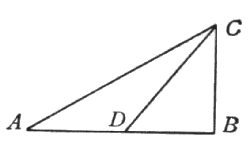
\includegraphics[width=6.25cm,height=3.65cm,keepaspectratio]{images/figura41.png} \end{center}
\end{center}

come, per intelligenza, essendo la linea \emph{AB} parallela all'orizonte, sopra 'l quale siano inclinati li due piani \emph{CA}, \emph{CD}, la perpendicolare \emph{CB}, cadente sopra l'orizontale \emph{BA}, chiama l'Autore la elevazione de i piani \emph{CA}, \emph{CD}; e suppone che i gradi di velocità del medesimo mobile scendente per li piani inclinati \emph{CA}, \emph{CD}, acquistati ne i termini \emph{A}, \emph{D}, siano eguali, per esser la loro elevazione l'istessa \emph{CB}: e tanto anco si deve intendere il grado di velocità che il medesimo cadente dal punto \emph{C} arebbe nel termine \emph{B}.

\speaker{Sagr.} Veramente mi par che tal supposto abbia tanto del probabile, che meriti di esser senza controversia conceduto, intendendo sempre che si rimuovano tutti gl'impedimenti accidentarii ed esterni, e che i piani siano ben solidi e tersi ed il mobile di figura perfettissimamente rotonda, sì che ed il piano ed il mobile non abbiano scabrosità. Rimossi tutti i contrasti ed impedimenti, il lume naturale mi detta senza difficoltà, che una palla grave e perfettamente rotonda, scendendo per le linee \emph{CA}, \emph{CD}, \emph{CB}, giugnerebbe ne i termini \emph{A}, \emph{D}, \emph{B} con impeti eguali.

\speaker{Salv.} Voi molto probabilmente discorrete; ma, oltre al verisimile, voglio con una esperienza accrescer tanto la probabilità, che poco gli manchi all'agguagliarsi ad una ben necessaria dimostrazione.


\begin{center}
\begin{center} 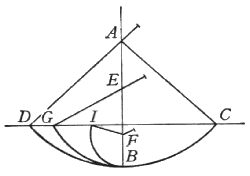
\includegraphics[width=6.25cm,height=4.40cm,keepaspectratio]{images/figura42.png} \end{center}
\end{center}

Figuratevi, questo foglio essere una parete eretta all'orizonte, e da un chiodo fitto in essa pendere una palla di piombo d'un'oncia o due, sospesa dal sottil filo \emph{AB}, lungo due o tre braccia, perpendicolare all'orizonte, e nella parete segnate una linea orizontale \emph{DC}, segante a squadra il perpendicolo \emph{AB}, il quale sia lontano dalla parete due dita in circa; trasferendo poi il filo \emph{AB} con la palla in \emph{AC}, lasciate essa palla in libertà: la quale primieramente vedrete scendere descrivendo l'arco \emph{CBD}, e di tanto trapassare il termine \emph{B}, che, scorrendo per l'arco \emph{BD}, sormonterà sino quasi alla segnata parallela \emph{CD}, restando di pervenirvi per piccolissimo intervallo, toltogli il precisamente arrivarvi dall'impedimento dell'aria e del filo; dal che possiamo veracemente concludere, che l'impeto acquistato nel punto \emph{B} dalla palla, nello scendere per l'arco \emph{CB}, fu tanto, che bastò a risospingersi per un simile arco \emph{BD} alla medesima altezza. Fatta e più volte reiterata cotale esperienza, voglio che ficchiamo nella parete, rasente al perpendicolo \emph{AB}, un chiodo, come in \emph{E} o vero in \emph{F}, che sporga in fuori cinque o sei dita, e questo acciò che il filo \emph{AC}, tornando, come prima, a riportar la palla \emph{C} per l'arco \emph{CB}, giunta che ella sia in \emph{B}, intoppando il filo nel chiodo \emph{E}, sia costretta a camminare per la circonferenza \emph{BG}, descritta intorno al centro \emph{E}; dal che vedremo quello che potrà far quel medesimo impeto che, dianzi, concepito nel medesimo termine \emph{B}, sospinse l'istesso mobile per l'arco \emph{BD} all'altezza della orizontale \emph{CD}. Ora, Signori, voi vedrete con gusto condursi la palla all'orizontale nel punto \emph{G}, e l'istesso accadere se l'intoppo si mettesse più basso, come in \emph{F}, dove la palla descriverebbe l'arco \emph{BI}, terminando sempre la sua salita precisamente nella linea \emph{CD}; e quando l'intoppo del chiodo fusse tanto basso che l'avanzo del filo sotto di lui non arrivasse all'altezza di \emph{CD} (il che accaderebbe quando fusse più vicino al punto \emph{B} che al segamento dell'\emph{AB} con l'orizontale \emph{CD}), allora il filo cavalcherebbe il chiodo e se gli avvolgerebbe intorno. Questa esperienza non lascia luogo di dubitare della verità del supposto: imperò che, essendo li due archi \emph{CB}, \emph{DB} eguali e similmente posti, l'acquisto di momento fatto per la scesa nell'arco \emph{CB} è il medesimo che il fatto per la scesa dell'arco \emph{DB}; ma il momento acquistato in \emph{B} per l'arco \emph{CB} è potente a risospingere in su il medesimo mobile per l'arco \emph{BD}; adunque anco il momento acquistato nella scesa \emph{DB} è eguale a quello che sospigne l'istesso mobile per il medesimo arco da \emph{B} in \emph{D}; sì che, universalmente, ogni momento acquistato per la scesa d'un arco è eguale a quello che può far risalire l'istesso mobile per il medesimo arco: ma i momenti tutti che fanno risalire per tutti gli archi \emph{BD}, \emph{BG}, \emph{BI} sono eguali, poiché son fatti dall'istesso medesimo momento acquistato per la scesa \emph{CB}, come mostra l'esperienza; adunque tutti i momenti che si acquistano per le scese ne gli archi \emph{DB}, \emph{GB}, \emph{IB} sono eguali.

\speaker{Sagr.} Il discorso mi par concludentissimo, e l'esperienza tanto accomodata per verificare il postulato, che molto ben sia degno d'esser conceduto come se fusse dimostrato.

\speaker{Salv.} Io non voglio, Sig. Sagredo, che noi ci pigliamo più del dovere, e massimamente che di questo assunto ci abbiamo a servire principalmente ne i moti fatti sopra superficie rette, e non sopra curve, nelle quali l'accelerazione procede con gradi molto differenti da quelli con i quali noi pigliamo ch'ella proceda ne' piani retti. Di modo che, se ben l'esperienza addotta ci mostra che la scesa per l'arco \emph{CB} conferisce al mobile momento tale, che può ricondurlo alla medesima altezza per qualsivoglia arco \emph{BD}, \emph{BG}, \emph{BI}, noi non possiamo con simile evidenza mostrare che l'istesso accadesse quando una perfettissima palla dovesse scendere per piani retti, inclinati secondo le inclinazioni delle corde di questi medesimi archi; anzi è credibile che, formandosi angoli da essi piani retti nel termine \emph{B}, la palla scesa per l'inclinato secondo la corda \emph{CB}, trovando intoppo ne i piani ascendenti secondo le corde \emph{BD}, \emph{BG}, \emph{BI}, nell'urtare in essi perderebbe del suo impeto, né potrebbe, salendo, condursi all'altezza della linea \emph{CD}: ma levato l'intoppo, che progiudica all'esperienza, mi par bene che l'intelletto resti capace, che l'impeto (che in effetto piglia vigore dalla quantità della scesa) sarebbe potente a ricondurre il mobile alla medesima altezza. Prendiamo dunque per ora questo come postulato, la verità assoluta del quale ci verrà poi stabilita dal vedere altre conclusioni, fabbricate sopra tale ipotesi, rispondere e puntualmente confrontarsi con l'esperienza. Supposto dall'Autore questo solo principio, passa alle proposizioni, dimostrativamente concludendole; delle quali la prima è questa:


\begin{center}
\begin{center} 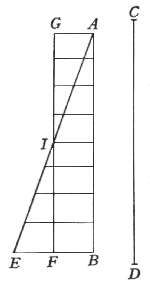
\includegraphics[width=3.75cm,height=7.08cm,keepaspectratio]{images/figura43.png} \end{center}
\end{center}

\textbf{TEOREMA 1. PROPOSIZIONE 1}\\ Il tempo in cui uno spazio dato è percorso da un mobile con moto uniformemente accelerato a partire dalla quiete, è eguale al tempo in cui quel medesimo spazio sarebbe percorso dal medesimo mobile mosso di moto equabile, il cui grado di velocità sia sudduplo [la metà] del grado di velocità ultimo e massimo [raggiunto dal mobile] nel precedente moto uniformemente accelerato.

\textbf{TEOREMA 2. PROPOSIZIONE 2}\\ Se un mobile scende, a partire dalla quiete, con moto uniformemente accelerato, gli spazi percorsi da esso in tempi qualsiasi stanno tra di loro in duplicata proporzione dei tempi [in un rapporto pari al rapporto dei tempi moltiplicato per se stesso], cioè stanno tra di loro come i quadrati dei tempi.

\textbf{COROLLARIO 1}\\ Di qui è manifesto che, se dal primo istante o inizio del moto avremo preso successivamente un numero qualsiasi di tempi eguali, come ad esempio AD, DE, EF, FG, nei quali siano percorsi gli spazi HL, LM, MN, NI, questi spazi staranno tra di loro come i numeri impari ab unitate, cioè come 1, 3, 5, 7: questa è infatti la proporzione tra gli eccessi dei quadrati delle linee che si eccedono egualmente e il cui eccesso è eguale alla minima di esse, o vogliam dire tra i numeri quadrati consecutivi ab unitate. Pertanto, mentre i gradi di velocità aumentano in tempi eguali secondo la serie dei numeri semplici, gli spazi percorsi nei medesimi tempi acquistano incrementi secondo la serie dei numeri impari ab unitate.

\speaker{Sagr.} Sospendete, in grazia, alquanto la lettura, mentre io vo ghiribizando intorno a certo concetto pur ora cascatomi in mente; per la spiegatura del quale, per mia e per vostra più chiara intelligenza, fo un poco di disegno.


\begin{center}
\begin{center} 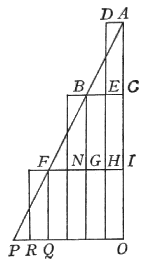
\includegraphics[width=3.75cm,height=6.60cm,keepaspectratio]{images/figura44.png} \end{center}
\end{center}

Dove mi figuro per la linea \emph{AI} la continuazione del tempo dopo il primo instante in \emph{A}; applicando poi in \emph{A}, secondo qualsivoglia angolo, la retta \emph{AF}, e congiugnendo i termini \emph{I}, \emph{F}, diviso il tempo \emph{AI} in mezo in \emph{C}, tiro la \emph{CB} parallela alla \emph{IF}; considerando poi la \emph{CB} come grado massimo della velocità che, cominciando dalla quiete nel primo instante del tempo \emph{A}, si andò augumentando secondo il crescimento delle parallele alla \emph{BC}, prodotte nel triangolo \emph{ABC} (che è il medesimo che crescere secondo che cresce il tempo), ammetto senza controversia, per i discorsi fatti sin qui, che lo spazio passato dal mobile cadente con la velocità accresciuta nel detto modo sarebbe eguale allo spazio che passerebbe il medesimo mobile quando si fusse nel medesimo tempo \emph{AC} mosso di moto uniforme, il cui grado di velocità fusse eguale all'\emph{EC}, metà del \emph{BC}. Passo ora più oltre, e figuratomi, il mobile sceso con moto accelerato trovarsi nell'instante \emph{C} avere il grado di velocità \emph{BC}, è manifesto, che se egli continuasse di muoversi con l'istesso grado di velocità \emph{BC} senza più accelerarsi, passerebbe nel seguente tempo \emph{CI} spazio doppio di quello che ei passò nell'egual tempo \emph{AC} col grado di velocità uniforme \emph{EC}, metà del grado \emph{BC}; ma perché il mobile scende con velocità accresciuta sempre uniformemente in tutti i tempi eguali, aggiugnerà al grado \emph{CB} nel seguente tempo \emph{CI} quei momenti medesimi di velocità crescente secondo le parallele del triangolo \emph{BFG}, eguale al triangolo \emph{ABC}: sì che, aggiunto al grado di velocità \emph{GI} la metà del grado \emph{FG}, massimo degli acquistati nel moto accelerato e regolati dalle parallele del triangolo \emph{BFG}, aremo il grado di velocità \emph{IN}, col quale di moto uniforme si sarebbe mosso nel tempo \emph{CI}; il qual grado \emph{IN} essendo triplo del grado \emph{EC}, convince, lo spazio passato nel secondo tempo \emph{CI} dovere esser triplo del passato nel primo tempo \emph{CA}. E se noi intenderemo, esser aggiunta all'\emph{AI} un'altra ugual parte di tempo \emph{IO}, ed accresciuto il triangolo sino in \emph{APO}, è manifesto, che quando si continuasse il moto per tutto 'l tempo \emph{IO} col grado di velocità \emph{IF}, acquistato nel moto accelerato nel tempo \emph{AI}, essendo tal grado \emph{IF} quadruplo dell'\emph{EC}, lo spazio passato nel tempo \emph{IO} sarebbe quadruplo del passato nell'egual primo tempo \emph{AC}; ma continuando l'accrescimento dell'uniforme accelerazione nel triangolo \emph{FPQ} simile a quello del triangolo \emph{ABC}, che ridotto a moto equabile aggiugne il grado eguale all'\emph{EC}, aggiunto il \emph{QR} eguale all'\emph{EC}, aremo tutta la velocità equabile esercitata nel tempo \emph{IO} quintupla dell'equabile del primo tempo \emph{AC}, e però lo spazio passato quintuplo del passato nel primo tempo \emph{AC}. Vedesi dunque anco in questo semplice calcolo, gli spazii passati in tempi uguali dal mobile che, partendosi dalla quiete, va acquistando velocità conforme all'accrescimento del tempo, esser tra di loro come i numeri impari \emph{ab unitate} 1, 3, 5, e, congiuntamente presi gli spazii passati, il passato nel doppio tempo esser quadruplo del passato nel sudduplo, il passato nel tempo triplo esser nonuplo, ed in somma gli spazii passati essere in duplicata proporzione de i tempi, cioè come i quadrati di essi tempi.

\speaker{Simp.} Io veramente ho preso più gusto in questo semplice e chiaro discorso del Sig. Sagredo, che nella per me più oscura dimostrazione dell'Autore; sì che io resto assai ben capace che il negozio deva succeder così, posta e ricevuta la definizione del moto uniformemente accelerato. Ma se tale sia poi l'accelerazione della quale si serve la natura nel moto de i suoi gravi descendenti, io per ancora ne resto dubbioso; e però, per intelligenza mia e di altri simili a me, parmi che sarebbe stato opportuno in questo luogo arrecar qualche esperienza di quelle che si è detto esservene molte, che in diversi casi s'accordano con le conclusioni dimostrate.

\speaker{Salv.} Voi, da vero scienziato, fate una ben ragionevol domanda; e così si costuma e conviene nelle scienze le quali alle conclusioni naturali applicano le dimostrazioni matematiche, come si vede ne i perspettivi, negli astronomi, ne i mecanici, ne i musici ed altri, li quali con sensate esperienze confermano i principii loro, che sono i fondamenti di tutta la seguente struttura: e però non voglio che ci paia superfluo se con troppa lunghezza aremo discorso sopra questo primo e massimo fondamento, sopra 'l quale s'appoggia l'immensa machina d'infinite conclusioni, delle quali solamente una piccola parte ne abbiamo in questo libro, poste dall'Autore, il quale arà fatto assai ad aprir l'ingresso e la porta stata sin or serrata agl'ingegni specolativi. Circa dunque all'esperienze, non ha tralasciato l'Autor di farne; e per assicurarsi che l'accelerazione de i gravi naturalmente descendenti segua nella proporzione sopradetta, molte volte mi son ritrovato io a farne la prova nel seguente modo, in sua compagnia.

In un regolo, o vogliàn dir corrente, di legno, lungo circa 12 braccia, e largo per un verso mezo bracio e per l'altro 3 dita, si era in questa minor larghezza incavato un canaletto, poco più largo d'un dito; tiratolo drittissimo, e, per averlo ben pulito e liscio, incollatovi dentro una carta pecora zannata e lustrata al possibile, si faceva in esso scendere una palla di bronzo durissimo, ben rotondata e pulita; costituito che si era il detto regolo pendente, elevando sopra il piano orizontale una delle sue estremità un braccio o due ad arbitrio, si lasciava (come dico) scendere per il detto canale la palla, notando, nel modo che appresso dirò, il tempo che consumava nello scorrerlo tutto, replicando il medesimo atto molte volte per assicurarsi bene della quantità del tempo, nel quale non si trovava mai differenza né anco della decima parte d'una battuta di polso. Fatta e stabilita precisamente tale operazione, facemmo scender la medesima palla solamente per la quarta parte della lunghezza di esso canale; e misurato il tempo della sua scesa, si trovava sempre puntualissimamente esser la metà dell'altro: e facendo poi l'esperienze di altre parti, esaminando ora il tempo di tutta la lunghezza col tempo della metà, o con quello delli duo terzi o de i 3/4, o in conclusione con qualunque altra divisione, per esperienze ben cento volte replicate sempre s'incontrava, gli spazii passati esser tra di loro come i quadrati e i tempi, e questo in tutte le inclinazioni del piano, cioè del canale nel quale si faceva scender la palla; dove osservammo ancora, i tempi delle scese per diverse inclinazioni mantener esquisitamente tra di loro quella proporzione che più a basso troveremo essergli assegnata e dimostrata dall'Autore. Quanto poi alla misura del tempo, si teneva una gran secchia piena d'acqua, attaccata in alto, la quale per un sottil cannellino, saldatogli nel fondo, versava un sottil filo d'acqua, che s'andava ricevendo con un piccol bicchiero per tutto 'l tempo che la palla scendeva nel canale e nelle sue parti: le particelle poi dell'acqua, in tal guisa raccolte, s'andavano di volta in volta con esattissima bilancia pesando, dandoci le differenze e proporzioni de i pesi loro le differenze e proporzioni de i tempi; e questo con tal giustezza, che, come ho detto, tali operazioni, molte e molte volte replicate, già mai non differivano d'un notabil momento.

\speaker{Simp.} Gran sodisfazione arei ricevuta nel trovarmi presente a tali esperienze: ma sendo certo della vostra diligenza nel farle e fedeltà nel referirle, mi quieto, e le ammetto per sicurissime e vere.

\speaker{Salv.} Potremo dunque ripigliar la nostra lettura, e seguitare avanti.

\textbf{COROLLARIO 2}\\ In secondo luogo si ricava che, se si prendono, a partire dall'inizio del moto, due spazi qualsiasi percorsi in tempi qualsiasi, i rispettivi tempi staranno tra di loro come uno dei due spazi sta al medio proporzionale tra i due spazi dati.

\textbf{SCOLIO}\\ Ora, quanto si è dimostrato riguardo ai moti verticali, si intenda verificarsi similmente anche nei moti sopra piani comunque inclinati: si è infatti assunto che, in questi ultimi, il grado di accelerazione aumenti sempre secondo la medesima proporzione, ossia secondo l'incremento del tempo, o vogliam dire secondo la prima serie semplice dei numeri.

\speaker{Salv.}\footnote{Il brano in forma di dialogo tra le interlinee, che Galileo voleva inserire in questo punto, è stato scritto dal suo discepolo Vincenzo Viviani (Firenze 1622--1703). [\emph{Nota per l extquotesingle edizione elettronica Manuzio}]} Qui vorrei, Sig. Sagredo, che a me ancora fosse permesso, se ben forsi con troppo tedio del Sig. Simplicio, il differir per un poco la presente lettura, fin ch'io possa esplicare quanto dal detto e dimostrato fin ora, e congiuntamente dalla notizia d'alcune conclusioni mecaniche apprese già dal nostro Academico, sovviemmi adesso di poter soggiugnere per maggior confermazione della verità del principio che sopra con probabili discorsi ed esperienze fu da noi esaminato, anzi, quello più importa, per geometricamente concluderlo, dimostrando prima un sol lemma, elementare nella contemplazione de gl'impeti.

\speaker{Sagr.} Mentre tale deva esser l'acquisto quale V. S. ci promette, non vi è tempo che da me volentierissimo non si spendesse, trattandosi di confermare e interamente stabilire queste scienze del moto: e quanto a me, non solo vi concedo il poter satisfarvi in questo particolare, ma di più pregovi ad appagare quanto prima la curiosità che mi avete in esso svegliata; e credo che il Sig. Simplicio abbia ancora il medesimo sentimento.

\speaker{Simp.} Non posso dire altrimenti.

\speaker{Salv.} Già che dunque me ne date licenza, considerisi in primo luogo, come effetto notissimo, che i momenti o le velocità d'un istesso mobile son diverse sopra diverse inclinazioni di piani, e che la massima è per la linea perpendicolarmente sopra l'orizonte elevata, e che per l'altre inclinate si diminuisce tal velocità, secondo che quelle più dal perpendicolo si discostano, cioè più obliquamente s'inclinano; onde l'impeto, il talento, l'energia, o vogliamo dire il momento, del descendere vien diminuito nel mobile dal piano soggetto, sopra il quale esso mobile s'appoggia e descende.


\begin{center}
\begin{center} 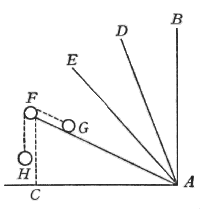
\includegraphics[width=5.00cm,height=5.25cm,keepaspectratio]{images/figura45.png} \end{center}
\end{center}

E per meglio dichiararmi, intendasi la linea \emph{AB}, perpendicolarmente eretta sopra l'orizonte \emph{AC}; pongasi poi la medesima in diverse inclinazioni verso l'orizonte piegata, come in \emph{AD}, \emph{AE}, \emph{AF}, etc.: dico, l'impeto massimo e totale del grave per descendere esser per la perpendicolare \emph{BA}, minor di questo per la \emph{DA}, e minore ancora per la \emph{EA}, e successivamente andarsi diminuendo per la più inclinata \emph{FA}, e finalmente esser del tutto estinto nella orizontale \emph{CA}, dove il mobile si trova indifferente al moto e alla quiete, e non ha per se stesso inclinazione di muoversi verso alcuna parte, né meno alcuna resistenza all'esser mosso; poiché, sì come è impossibile che un grave o un composto di essi si muova naturalmente all'in su, discostandosi dal comun centro verso dove conspirano tutte le cose gravi, così è impossibile che egli spontaneamente si muova, se con tal moto il suo proprio centro di gravità non acquista avvicinamento al sudetto centro comune: onde sopra l'orizontale, che qui s'intende per una superficie egualmente lontana dal medesimo centro, e perciò affatto priva d'inclinazione, nullo sarà l'impeto o momento di detto mobile.

Appresa questa mutazione d'impeto, mi fa qui mestier esplicare quello che in un antico trattato di mecaniche, scritto già in Padova dal nostro Academico sol per uso de' suoi discepoli, fu diffusamente e concludentemente dimostrato, in occasione di considerare l'origine e natura del maraviglioso strumento della vita; ed è con qual proporzione si faccia tal mutazione d'impeto per diverse inclinazioni di piani: come, per esempio, del piano inclinato \emph{AF} tirando la sua elevazione sopra l'orizonte, cioè la linea \emph{FC}, per la quale l'impeto d'un grave ed il momento del descendere è il massimo, cercasi qual proporzione abbia questo momento al momento dell'istesso mobile per l'inclinata \emph{FA}; qual proporzione dico esser reciproca delle dette lunghezze: e questo sia il lemma da premettersi al teorema, che dopo io spero di poter dimostrare. Qui è manifesto, tanto essere l'impeto del descendere d'un grave, quanta è la resistenza o forza minima che basta per proibirlo e fermarlo: per tal forza e resistenza, e sua misura, mi voglio servire della gravità d'un altro mobile. Intendasi ora, sopra il piano \emph{FA} posare il mobile \emph{G}, legato con un filo che, cavalcando sopra l'\emph{F}, abbia attaccato un peso \emph{H}; e consideriamo che lo spazio della scesa o salita a perpendicolo di esso è ben sempre eguale a tutta la salita o scesa dell'altro mobile \emph{G} per l'inclinata \emph{AF}, ma non già alla salita o scesa a perpendicolo, nella qual sola esso mobile \emph{G} (sì come ogn'altro mobile) esercita la sua resistenza. Il che è manifesto. Imperoché considerando, nel triangolo \emph{AFC} il moto del mobile \emph{G}, per esempio all'in su da \emph{A} in \emph{F}, esser composto del trasversale orizontale \emph{AC} e del perpendicolare \emph{CF}; ed essendo che quanto all'orizontale, nessuna, come s'è detto, è la resistenza del medesimo all'esser mosso (non facendo con tal moto perdita alcuna, né meno acquisto, in riguardo della propria distanza dal comun centro delle cose gravi, che nell'orizonte si conserva sempre l'istessa); resta, la resistenza esser solamente rispetto al dover salire la perpendicolare \emph{CF}. Mentre che dunque il grave \emph{G}, movendosi da \emph{A} in \emph{F}, resiste solo, nel salire, lo spazio perpendicolare \emph{CF}, ma che l'altro grave \emph{H} scende a perpendicolo necessariamente quanto tutto lo spazio \emph{FA}, e che tal proporzione di salita e scesa si mantien sempre l'istessa, poco o molto che sia il moto de i detti mobili (per esser collegati insieme); possiamo assertivamente affermare, che quando debba seguire l'equilibrio, cioè la quiete tra essi mobili, i momenti, le velocità, o le lor propensioni al moto, cioè gli spazii che da loro si passerebbero nel medesimo tempo, devon rispondere reciprocamente alle loro gravità, secondo quello che in tutti i casi de' movimenti mecanici si dimostra: sì che basterà, per impedire la scesa del \emph{G}, che lo \emph{H} sia tanto men grave di quello, quanto a proporzione lo spazio \emph{CF} è minore dello spazio \emph{FA}. Sia fatto, dunque, come \emph{FA} ad \emph{FC}, così il grave \emph{G} al grave \emph{H}; ché allora seguirà l'equilibrio, cioè i gravi \emph{H}, \emph{G} averanno momenti eguali, e cesserà il moto de i detti mobili. E perché siamo convenuti, che di un mobile tanto sia l'impeto, l'energia, il momento, o la propensione al moto, quanta è la forza o resistenza minima che basta a fermarlo, e s'è concluso che il grave \emph{H} è bastante a proibire il moto al grave \emph{G}, adunque il minor peso \emph{H}, che nella perpendicolare \emph{FC} esercita il suo momento totale, sarà la precisa misura del momento parziale che il maggior peso \emph{G} esercita per il piano inclinato \emph{FA}; ma la misura del total momento del medesimo grave \emph{G} è egli stesso (poiché per impedire la scesa perpendicolare d'un grave si richiede il contrasto d'altrettanto grave, che pur sia in libertà di muoversi perpendicolarmente); adunque l'impeto o momento parziale del \emph{G} per l'inclinata \emph{FA}, all'impeto massimo e totale dell'istesso \emph{G} per la perpendicolare \emph{FC}, starà come il peso \emph{H} al peso \emph{G}, cioè, per la costruzione, come essa perpendicolare \emph{FC}, elevazione dell'inclinata, alla medesima inclinata \emph{FA}: che è quello che per lemma si propose di dimostrare, e che dal nostro Autore, come vedranno, vien supposto per noto nella seconda parte della sesta proposizione del presente trattato.

\speaker{Sagr.} Da questo che V. S. ha concluso fin qui, parmi che facilmente si possa dedurre, argumentando \emph{ex æquali} con la proporzione perturbata, che i momenti dell'istesso mobile per piani diversamente inclinati, come \emph{FA}, \emph{FI}, che abbino l'istessa elevazione, son fra loro in reciproca proporzione de' medesimi piani.

\speaker{Salv.} Verissima conclusione. Fermato questo, passerò adesso a dimostrare il teorema, cioè che:


\begin{enunciato}
I gradi di velocità d'un mobile descendente con moto naturale dalla medesima sublimità per piani in qualsivoglia modo inclinati, all'arrivo all'orizonte son sempre eguali, rimossi gl'impedimenti.
\end{enunciato}

Qui devesi prima avvertire, che stabilito che in qualsivoglino inclinazioni il mobile dalla partita dalla quiete vada crescendo la velocità, o la quantità dell'impeto, con la proporzione del tempo (secondo la definizione data dall'Autore al moto naturalmente accelerato), onde, com'egli ha per l'antecedente proposizione dimostrato, gli spazii passati sono in duplicata proporzione de' tempi, e conseguentemente de' gradi di velocità; quali furono gl'impeti nella prima mossa, tali proporzionalmente saranno i gradi delle velocità guadagnati nell'istesso tempo, poiché e questi e quelli crescono con la medesima proporzione nel medesimo tempo.


\begin{center}
\begin{center} 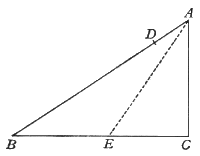
\includegraphics[width=5.00cm,height=3.90cm,keepaspectratio]{images/figura46.png} \end{center}
\end{center}

Ora sia il piano inclinato \emph{AB}, la sua elevazione sopra l'orizonte la perpendicolare \emph{AC}, e l'orizontale \emph{CB}; e perché, come poco fa si è concluso, l'impeto d'un mobile per la perpendicolare \emph{AC}, all'impeto del medesimo per l'inclinata \emph{AB}, sta come \emph{AB} ad \emph{AC}, prendasi nell'inclinata \emph{AB} la \emph{AD}, terza proporzionale delle \emph{AB}, \emph{AC}: l'impeto dunque per \emph{AC} all'impeto per la \emph{AB}, cioè per la \emph{AD}, sta come la \emph{AC} all'\emph{AD}; e perciò il mobile nell'istesso tempo che passerebbe lo spazio perpendicolare \emph{AC}, passerà ancora lo spazio \emph{AD} nell'inclinata \emph{AB} (essendo i momenti come gli spazii), ed il grado di velocità in \emph{C} al grado di velocità in \emph{D} averà la medesima proporzione della \emph{AC} alla \emph{AD}. Ma il grado di velocità in \emph{B} al medesimo grado in \emph{D} sta come il tempo per \emph{AB} al tempo per \emph{AD}, per la definizione del moto accelerato, ed il tempo per \emph{AB} al tempo per \emph{AD} sta come la medesima \emph{AC}, media tra le \emph{BA}, \emph{AD}, alla \emph{AD}, per l'ultimo corollario della seconda proposizione; adunque i gradi in \emph{B} ed in \emph{C} al grado in \emph{D} hanno la medesima proporzione della \emph{AC} alla \emph{AD}, e però sono eguali: che è il teorema che intesi di dimostrare.

Da questo potremo più concludentemente provare la seguente terza proposizione dell'Autore, nella quale egli si vale del principio; ed è che il tempo per l'inclinata al tempo per la perpendicolare ha l'istessa proporzione di essa inclinata e perpendicolare. Imperoché diciamo: quando \emph{BA} sia il tempo per \emph{AB}, il tempo per \emph{AD} sarà la media tra esse, cioè la \emph{AC}, per il secondo corollario della seconda proposizione; ma quando \emph{AC} sia il tempo per \emph{AD}, sarà anco il tempo per \emph{AC}, per essere le \emph{AD}, \emph{AC} scorse in tempi eguali; e però quando \emph{BA} sia il tempo per \emph{AB}, \emph{AC} sarà il tempo per \emph{AC}; adunque, come \emph{AB} ad \emph{AC}, così il tempo per \emph{AB} al tempo per \emph{AC}.

Col medesimo discorso si proverà, che il tempo per \emph{AC} al tempo per altra inclinata \emph{AE} sta come la \emph{AC} alla \emph{AE}; adunque, \emph{ex æquali}, il tempo per l'inclinata \emph{AB} al tempo dell'inclinata \emph{AE} sta omologamente come la \emph{AB} alla \emph{AE}, etc.

Potevasi ancora dall'istesso progresso del teorema, come vedrà benissimo il Sig. Sagredo, dimostrar immediatamente la sesta proposizione dell'Autore: ma basti per ora tal digressione, che forsi gli è riuscita troppo tediosa, benché veramente di profitto in queste materie del moto.

\speaker{Sagr.} Anzi di mio grandissimo gusto, e necessarissima alla perfetta intelligenza di quel principio.

\speaker{Salv.} Ripiglierò dunque la lettura del testo.

\textbf{TEOREMA 3. PROPOSIZIONE 3}\\ Se un medesimo mobile si muove, a partire dalla quiete, su un piano inclinato e lungo una perpendicolare, che abbiano eguale altezza, i tempi dei moti staranno tra di loro come le lunghezze [\emph{rispettivamente}] del piano e della perpendicolare.


\begin{center}
\begin{center} 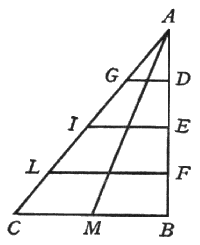
\includegraphics[width=5.00cm,height=6.12cm,keepaspectratio]{images/figura47.png} \end{center}
\end{center}

\speaker{Sagr.} Parmi che assai chiaramente e con brevità si poteva concludere il medesimo, essendosi già concluso che la somma del moto accelerato de i passaggi per \emph{AC}, \emph{AB} è quanto il moto equabile il cui grado di velocità sia sudduplo al grado massimo \emph{CB}; essendo dunque passati li due spazii \emph{AC}, \emph{AB} con l'istesso moto equabile, già è manifesto, per la proposizione prima del primo, che i tempi de' passaggi saranno come gli spazii medesimi.

\textbf{COROLLARIO}\\ Di qui si ricava che i tempi impiegati a scendere su piani diversamente inclinati, purché però abbiano la medesima elevazione, stanno tra di loro come le rispettive lunghezze.

\textbf{TEOREMA 4. PROPOSIZIONE 4}\\ I tempi dei moti su piani di eguale lunghezza, ma di diversa inclinazione, stanno tra di loro in sudduplicata proporzione delle elevazioni dei medesimi piani permutatamente prese [\emph{in un rapporto pari alla radice quadrata del rapporto inverso tra le elevazioni}].

\textbf{TEOREMA 5. PROPOSIZIONE 5}\\ La proporzione tra i tempi delle discese su piani di diversa inclinazione e lunghezza e di elevazione pure diseguale, è composta dalla proporzione tra le rispettive lunghezze e della sudduplicata proporzione delle elevazioni permutatamente prese.


\begin{center}
\begin{center} 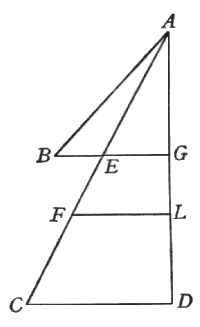
\includegraphics[width=5.00cm,height=8.18cm,keepaspectratio]{images/figura48.png} \end{center}
\end{center}

\textbf{TEOREMA 6. PROPOSIZIONE 6}\\ Se dal più alto o dal più basso punto di un cerchio eretto sull'orizzonte si conducono piani inclinati qualsiasi fino alla circonferenza, i tempi delle discese lungo tali piani saranno eguali.

\textbf{COROLLARIO 1}\\ Di qui si ricava che i tempi delle discese lungo tutte le corde condotte dagli estremi \emph{C} o \emph{D}, sono tra di loro eguali.

\textbf{COROLLARIO 2}\\ Si ricava inoltre che, se da un medesimo punto partono una perpendicolare e un piano inclinato tali, che i tempi di discesa lungo di essi siano eguali, quella perpendicolare e quel piano inclinato risultano [inscrivibili] in un semicerchio, il cui diametro è la perpendicolare medesima.


\begin{center}
\begin{center} 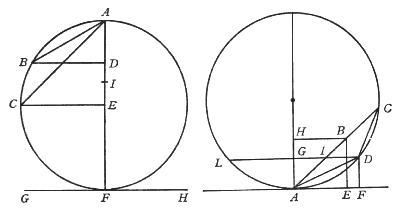
\includegraphics[width=10.00cm,height=5.25cm,keepaspectratio]{images/figura49.png} \end{center}
\end{center}

\textbf{COROLLARIO 3}\\ Si ricava anche che i tempi dei moti sopra piani inclinati sono eguali allorché le elevazioni di tratti eguali di tali piani staranno tra di esse come le lunghezze dei piani medesimi: si è infatti mostrato, nella penultima\footnote{In realtà, avendo l extquotesingle edizione U.T.E.T. omesso una dimostrazione, ci si riferisce qui all extquotesingle ultima figura. [\emph{Nota per l extquotesingle edizione elettronica Manuzio}]} figura, che i tempi delle discese per \emph{CA} e \emph{DA} sono eguali, quando l'elevazione del tratto \emph{AB}, eguale ad \emph{AD}, ossia \emph{BE}, sta alla elevazione \emph{DF} come \emph{CA} sta a \emph{DA}.

\speaker{Sagr.} Sospenda in grazia V. S. per un poco la lettura delle cose che seguono, sin che io mi vo risolvendo sopra certa contemplazione che pur ora mi si rivolge per la mente; la quale, quando non sia una fallacia, non è lontana dall'essere uno scherzo grazioso, quali sono tutti quelli della natura o della necessità.

È manifesto, che se da un punto segnato in un piano orizontale si faranno produr sopra 'l medesimo piano infinite linee rette per tutti i versi, sopra ciascuna delle quali s'intenda muoversi un punto con moto equabile, cominciandosi a muover tutti nell'istesso momento di tempo dal segnato punto, e che siano le velocità di tutti eguali, si verranno conseguentemente a figurar da essi punti mobili circonferenze di cerchi, tuttavia maggiori e maggiori, concentrici tutti intorno al primo punto segnato; giusto in quella maniera che vediamo farsi dall'ondette dell'acqua stagnante, dopo che da alto vi sia caduto un sassetto, la percossa del quale serve per dar principio di moto verso tutte le parti, e resta come centro di tutti i cerchi che vengon disegnati, successivamente maggiori e maggiori, da esse ondette. Ma se noi intenderemo un piano eretto all'orizonte, ed in esso piano notato un punto sublime, dal quale si portano infinite linee inclinate secondo tutte le inclinazioni, sopra le quali ci figuriamo descender mobili gravi, ciascheduno con moto naturalmente accelerato, con quelle velocità che alle diverse inclinazioni convengono; posto che tali mobili descendenti fusser continuamente visibili, in che sorti di linee gli vedremmo noi continuamente disposti? Qui nasce la mia maraviglia, mentre le precedenti dimostrazioni mi assicurano che si vedranno sempre tutti nell'istessa circonferenza di cerchi successivamente crescenti, secondo che i mobili nello scendere si vanno più e più successivamente allontanando dal punto sublime, dove fu il principio della lor caduta.


\begin{center}
\begin{center} 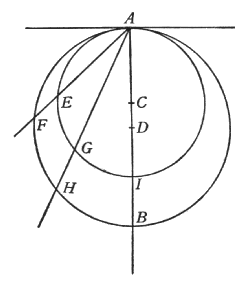
\includegraphics[width=6.25cm,height=7.15cm,keepaspectratio]{images/figura50.png} \end{center}
\end{center}

E per meglio dichiararmi, segnisi il punto subblime \emph{A}, dal quale descendano linee secondo qualsivogliano inclinazioni \emph{AF}, \emph{AH}, e la perpendicolare \emph{AB}, nella quale presi i punti \emph{C}, \emph{D} descrivansi intorno ad essi cerchi che passino per il punto \emph{A}, segando le linee inclinate ne i punti \emph{F}, \emph{H}, \emph{B}, \emph{E}, \emph{G}, \emph{I}: è manifesto, per le antecedenti dimostrazioni, che partendosi nell'istesso tempo dal termine \emph{A} mobili descendenti per esse linee, quando l'uno sarà in \emph{E}, l'altro sarà in \emph{G} e l'altro in \emph{I}; e così, continuando di scendere, si troveranno nell'istesso momento di tempo in \emph{F}, \emph{H}, \emph{B}; e continuando di muoversi questi ed altri infiniti per le infinite diverse inclinazioni, si troveranno sempre successivamente nelle medesime circonferenze, fatte maggiori e maggiori in infinito. Dalle due specie dunque di moti, delle quali la natura si serve, nasce con mirabil corrispondente diversità la generazione di cerchi infiniti: quella si pone, come in sua sede e principio originario, nel centro d'infiniti cerchi concentrici; questa si costituisce nel contatto subblime delle infinite circonferenze di cerchi, tutti tra loro eccentrici: quelli nascono da moti tutti eguali ed equabili; questi, da moti tutti sempre inequabili in se stessi, e diseguali l'uno dall'altro tutti, che sopra le differenti infinite inclinazioni si esercitano. Ma più aggiunghiamo, che se da i due punti assegnati per le emanazioni noi intenderemo eccitarsi linee non per due superficie sole, orizontale ed eretta, ma per tutti i versi, sì come da quelle, cominciandosi da un sol punto, si passava alla produzzione di cerchi, dal minimo al massimo, così, cominciandosi da un sol punto, si verranno producendo infinite sfere, o vogliam dire una sfera che in infinite grandezze si andrà ampliando, e questo in due maniere: cioè, o col por l'origine nel centro, o vero nella circonferenza di tali sfere.

\speaker{Salv.} La contemplazione è veramente bellissima, e proporzionata all'ingegno del Sig. Sagredo.

\speaker{Simp.} Io, restando al meno capace della contemplazione sopra le due maniere del prodursi, con li due diversi moti naturali, i cerchi e le sfere, se bene della produzzione dependente dal moto accelerato e della sua dimostrazione non son del tutto intelligente, tuttavia quel potersi assegnare per luogo di tale emanazione tanto il centro infimo quanto l'altissima sferica superficie, mi fa credere che possa essere che qualche gran misterio si contenga in queste vere ed ammirande conclusioni; misterio, dico, attenente alla creazione dell'universo, il quale si stima essere di forma sferica, ed alla residenza della prima causa.

\speaker{Salv.} Io non ho repugnanza al creder l'istesso. Ma simili profonde contemplazioni si aspettano a più alte dottrine che le nostre: ed a noi deve bastare d'esser quei men degni artefici, che dalle fodine scuoprono e cavano i marmi, ne i quali poi gli scultori industri fanno apparire maravigliose immagini, che sotto roza ed informe scorza stavano ascoste. Or, se così vi piace, seguiremo avanti.

\textbf{TEOREMA 7. PROPOSIZIONE 7}\\ Se le elevazioni di due piani avranno tra di loro una proporzione doppia di quella posseduta dalle lunghezze dei medesimi piani, su di questi i moti a partire dalla quiete si compiranno in tempi eguali.

\textbf{TEOREMA 8. PROPOSIZIONE 8}\\ Tra i piani delimitati da un medesimo cerchio eretto sull'orizzonte, su quelli, che terminano nell'estremo inferiore o superiore del diametro perpendicolare, i tempi delle discese sono eguali al tempo della caduta lungo il diametro; invece sui piani che non raggiungono il diametro, i tempi sono più brevi; infine, sui piani che tagliano il diametro, sono più lunghi.


\begin{center}
\begin{center} 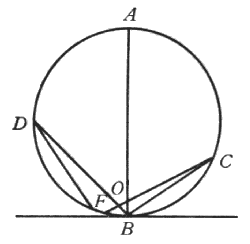
\includegraphics[width=6.25cm,height=6.10cm,keepaspectratio]{images/figura51.png} \end{center}
\end{center}

\textbf{TEOREMA 9. PROPOSIZIONE 9}\\ Se a partire da un punto di una linea parallela all'orizzonte si conducono due piani comunque inclinati, e questi sono tagliati da una linea, che formi con essi angoli permutatamente [\emph{inversamente}] eguali agli angoli racchiusi dai medesimi piani e dalla orizzontale, i moti lungo i tratti intersecati dalla suddetta linea si compiranno in tempi eguali.

\textbf{TEOREMA 10. PROPOSIZIONE 10}\\ I tempi dei moti sopra piani di diversa inclinazione ma di elevazione eguale, stanno tra di loro come le lunghezze dei piani medesimi, sia che i moti si svolgano a partire dalla quiete, sia che li preceda un moto [\emph{iniziato}] da una medesima altezza [\emph{cfr. figura 48}].

\textbf{TEOREMA 11. PROPOSIZIONE 11}\\ Se il piano, sul quale si svolge il moto a partire dalla quiete, viene diviso in un modo qualsiasi, il tempo del moto lungo il primo tratto sta al tempo del moto lungo il tratto successivo, come quel medesimo primo tratto sta all'eccesso che, su di esso, ha la media proporzionale tra l'intero piano e il suo primo tratto.

\textbf{TEOREMA 12. PROPOSIZIONE 12}


\begin{center}
\begin{center} 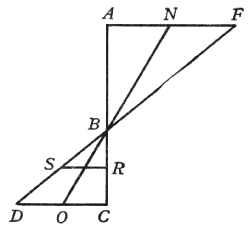
\includegraphics[width=6.25cm,height=5.70cm,keepaspectratio]{images/figura52.png} \end{center}
\end{center}

Se una perpendicolare e un piano comunque inclinato si intersecano tra di loro [nello spazio compreso] tra due medesime linee orizzontali, e se si prendono le medie proporzionali tra ciascuno di essi e la rispettiva parte compresa tra il punto comune di intersezione e la linea orizzontale superiore, il tempo del moto lungo la perpendicolare starà al tempo del moto [complessivo] lungo la parte superiore della perpendicolare e poi lungo la parte inferiore del piano secante, nella medesima proporzione che l'intera lunghezza della perpendicolare ha alla linea composta della media proporzionale presa sulla perpendicolare, e dell'eccesso dell'intero piano inclinato sulla propria media proporzionale.

\textbf{PROBLEMA 1. PROPOSIZIONE 13}\\ Data una perpendicolare, condurre ad essa un piano inclinato tale, che, avendo esso elevazione eguale a quella della perpendicolare, il moto su di esso dopo la caduta lungo la perpendicolare si compia in un tempo eguale a quello della caduta lungo la perpendicolare data a partire dalla quiete.

\textbf{PROBLEMA 2. PROPOSIZIONE 14}\\ Data una perpendicolare e dato un piano ad essa inclinato, determinare nella parte superiore della perpendicolare un tratto tale, che il tempo impiegato a percorrerlo a partire dalla quiete risulti eguale al tempo impiegato a percorrere il piano inclinato con moto successivo alla caduta lungo il suddetto tratto di perpendicolare.

\textbf{PROBLEMA 3. PROPOSIZIONE 15}\\ Dati una perpendicolare e un piano ad essa inclinato, determinare sul prolungamento inferiore della perpendicolare un tratto tale, che il tempo impiegato a percorrerlo risulti eguale al tempo impiegato a percorrere il piano inclinato con moto successivo alla caduta lungo la perpendicolare data.


\begin{center}
\begin{center} 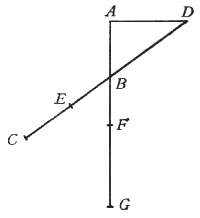
\includegraphics[width=5.00cm,height=5.45cm,keepaspectratio]{images/figura53.png} \end{center}
\end{center}

\textbf{TEOREMA 13. PROPOSIZIONE 16}\\ Se in un punto convergono i tratti di un piano inclinato e di una perpendicolare, tali che risultino eguali i tempi dei moti lungo di essi a partire dalla quiete, un mobile che cada da una qualsiasi altezza più elevata percorrerà più presto il tratto del piano inclinato che non quello della perpendicolare.

\textbf{COROLLARIO}\\ Da questa e dalla precedente proposizione si ricava che, dopo una caduta dall'alto, lo spazio, che viene percorso lungo la perpendicolare nel medesimo tempo impiegato a percorrere un dato piano inclinato, è minore dello spazio che viene percorso in tempo eguale a quello impiegato a percorrere il piano inclinato senza una precedente caduta dall'alto; tuttavia è maggiore del piano inclinato stesso.

\textbf{PROBLEMA 4. PROPOSIZIONE 17}\\ Dati una perpendicolare e un piano ad essa inclinato, segnare su questo un tratto tale, che un mobile, dopo essere caduto lungo la perpendicolare data, lo percorra in un tempo eguale a quello impiegato a percorrere la medesima perpendicolare a partire dalla quiete.


\begin{center}
\begin{center} 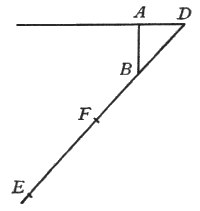
\includegraphics[width=5.00cm,height=5.28cm,keepaspectratio]{images/figura54.png} \end{center}
\end{center}

\textbf{PROBLEMA 5. PROPOSIZIONE 18}\\ Preso sulla perpendicolare, dall'inizio del moto, uno spazio qualsiasi, il quale sia percorso in un dato tempo, e dato un altro tempo minore qualsiasi, determinare, sulla medesima perpendicolare, un altro spazio [\emph{eguale in lunghezza al precedente}], il quale venga percorso nel tempo minore dato.


\begin{center}
\begin{center} 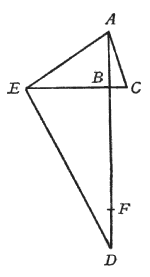
\includegraphics[width=3.75cm,height=6.93cm,keepaspectratio]{images/figura55.png} \end{center}
\end{center}

\textbf{PROBLEMA 6. PROPOSIZIONE 19}\\ Dato su una perpendicolare uno spazio qualsiasi percorso dall'inizio del moto, e dato il tempo della caduta, trovare il tempo in cui il medesimo mobile percorre successivamente un altro spazio eguale, preso in una parte qualsiasi della medesima perpendicolare.

\textbf{COROLLARIO}


\begin{center}
\begin{center} 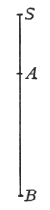
\includegraphics[width=1.25cm,height=5.25cm,keepaspectratio]{images/figura56.png} \end{center}
\end{center}

Di qui si ricava che, se si pone che il tempo, impiegato a percorrere un qualche spazio a partire dalla quiete, sia eguale allo spazio stesso, il tempo impiegato a percorrerlo, dopo che si sia già percorso un altro spazio, sarà eguale all'eccesso del medio proporzionale tra la somma dello spazio aggiunto più lo spazio dato e il medesimo spazio dato, sul medio proporzionale tra il primo spazio e lo spazio aggiunto: ad esempio, posto che il tempo del moto per \emph{AB} a partire dalla quiete in \emph{A} sia \emph{AB}, qualora si aggiunga lo spazio \emph{AS}, il tempo del moto per \emph{AB} dopo il moto per \emph{SA} sarà eguale all'eccesso del medio proporzionale tra \emph{SB} e \emph{BA} sul medio proporzionale tra \emph{BA} e \emph{AS}.

\textbf{PROBLEMA 7. PROPOSIZIONE 20}\\ Dato uno spazio qualsiasi e preso su di esso un tratto a partire dall'inizio del moto, determinare un altro tratto, alla fine [del moto], che sia percorso nello stesso tempo del primo tratto dato.

\textbf{TEOREMA 14. PROPOSIZIONE 21}\\ Se ha luogo una caduta lungo la perpendicolare a partire dalla quiete, e se si prende, dall'inizio del moto, un tratto, percorso in un tempo qualsiasi, cui segua un moto deviato su un piano comunque inclinato, lo spazio che, su tale piano, viene percorso in un tempo eguale a quello della caduta precedentemente svoltasi lungo la perpendicolare, sarà più del doppio, ma meno del triplo, dello spazio già percorso lungo la perpendicolare.

\textbf{PROBLEMA 8. PROPOSIZIONE 22}\\ Dati due tempi diseguali, e dato lo spazio che viene percorso lungo la perpendicolare a partire dalla quiete nel più breve dei due tempi dati, condurre dall'estremo superiore della perpendicolare fino all'orizzonte un piano inclinato, sul quale il mobile scenda in un tempo eguale al più lungo dei tempi dati.

\textbf{PROBLEMA 9. PROPOSIZIONE 23}


\begin{center}
\begin{center} 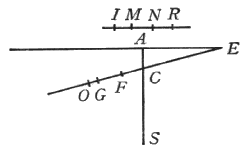
\includegraphics[width=6.25cm,height=3.88cm,keepaspectratio]{images/figura57.png} \end{center}
\end{center}

Preso sulla perpendicolare uno spazio percorso in un tempo qualsiasi a partire dalla quiete, condurre dall'estremo inferiore di questo spazio un piano inclinato, sul quale, dopo la caduta lungo la perpendicolare, venga percorso nel medesimo tempo uno spazio eguale a uno spazio dato qualsiasi, purché superiore al doppio, ma inferiore al triplo, dello spazio percorso lungo la perpendicolare.

\textbf{SCOLIO}


\begin{center}
\begin{center} 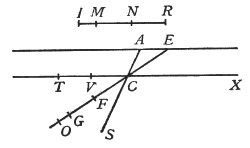
\includegraphics[width=6.25cm,height=3.70cm,keepaspectratio]{images/figura58.png} \end{center}
\end{center}

Se si considera attentamente, apparirà manifesto che, quanto meno manca alla linea data \emph{IR} per raggiungere il triplo della \emph{AC}, tanto maggiormente il piano inclinato, sul quale deve svolgersi il secondo movimento, come ad esempio \emph{CO}, si avvicina alla perpendicolare, e finalmente, lungo quest'ultima, viene percorso in un tempo eguale ad \emph{AC} uno spazio che è tre volte \emph{AC}. Infatti, allorché \emph{IR} sarà prossima al triplo di \emph{AC}, \emph{IM} sarà quasi eguale ad \emph{MN}; e poiché, per costruzione, come \emph{IM} sta ad \emph{MN} così \emph{AC} sta a \emph{CE}, ne risulta che la medesima \emph{CE} si trova ad essere di poco maggiore della \emph{CA}, e, di conseguenza, il punto \emph{E} si trova ad essere prossimo al punto \emph{A}, e \emph{CO} forma con \emph{CS} un angolo molto acuto, coincidendo quasi l'una con l'altra. Viceversa, se la linea data \emph{IR} sarà di pochissimo superiore al doppio della medesima \emph{AC}, \emph{IM} sarà una linea brevissima; ne verrà che anche la \emph{AC} sarà minima rispetto alla \emph{CE}, la quale sarà lunghissima e quanto più prossima alla parallela orizzontale passante per \emph{C}. E di qui possiamo ricavare che, se nella figura accanto dopo la discesa sul piano inclinato \emph{AC} il moto viene riflesso lungo la linea orizzontale, quale sarebbe \emph{CT}, lo spazio che il mobile successivamente percorrerebbe in un tempo eguale al tempo della discesa per \emph{AC}, sarebbe esattamente doppio dello spazio \emph{AC}. Sembra inoltre che qui sia anche adatto un consimile ragionamento: infatti, è chiaro, dal fatto che \emph{OE} sta ad \emph{EF} come \emph{FE} ad \emph{EC}, che proprio la \emph{FC} determina il tempo della discesa per \emph{CO}. Se poi il tratto orizzontale \emph{TC}, doppio di \emph{CA}, vien diviso a metà in \emph{V}, prolungato verso \emph{X} si estenderà all'infinito prima che possa incontrare il prolungamento di \emph{AE}, e la proporzione della linea infinita \emph{TX} all'infinita \emph{VX} non sarà diversa dalla proporzione dell'infinita \emph{VX} all'infinita \emph{XC}.

A questa stessa conclusione saremmo potuti giungere seguendo un altro procedimento, rifacendo un ragionamento consimile a quello seguìto nella dimostrazione della proposizione prima.


\begin{center}
\begin{center} 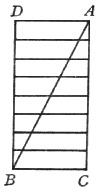
\includegraphics[width=2.50cm,height=4.80cm,keepaspectratio]{images/figura59.png} \end{center}
\end{center}

Riprendiamo, infatti, il triangolo \emph{ABC}, che sulle parallele alla base \emph{BC} ci rappresenta i gradi di velocità continuamente aumentati secondo il crescere del tempo, le quali [parallele], essendo infinite, siccome infiniti sono i punti nella linea \emph{AC} e gli istanti in un tempo qualsiasi, daranno origine alla superficie stessa del triangolo; se intendiamo che il moto continui per altrettanto tempo, ma non più accelerato, bensì equabile, secondo il massimo grado della velocità acquistata, il quale grado è rappresentato dalla linea \emph{BC}; tali gradi di velocità formeranno un aggregato simile al parallelogramma \emph{ADBC}, che è doppio del triangolo \emph{ABC}: perciò lo spazio percorso nel medesimo tempo con gradi di velocità consimili [\emph{tutti eguali a BC}], sarà doppio dello spazio percorso coi gradi di velocità rappresentati dal triangolo \emph{ABC}. Ma su un piano orizzontale il moto è equabile, allorché non intervenga nessuna causa di accelerazione o di ritardamento; dunque, si conclude che lo spazio \emph{CD} percorso in un tempo eguale al tempo \emph{AC} è doppio dello spazio \emph{AC}: infatti quest'ultimo viene percorso con moto accelerato a partire dalla quiete, secondo le parallele del triangolo; quello, invece, secondo le parallele del parallelogramma, le quali, quando siano prese nella loro infinità, risultano doppie delle infinite parallele del triangolo.

Inoltre, è lecito aspettarsi che, qualunque grado di velocità si trovi in un mobile, gli sia per sua natura indelebilmente impresso, purché siano tolte le cause esterne di accelerazione o di ritardamento; il che accade soltanto nel piano orizzontale; infatti nei piani declivi è di già presente una causa di accelerazione, mentre in quelli acclivi [è già presente una causa] di ritardamento: da ciò segue parimenti che il moto sul piano orizzontale è anche eterno; infatti, se è equabile, non scema o diminuisce, né tanto meno cessa. E per di più, poiché esiste un grado di velocità acquistato dal mobile nella discesa naturale, e poiché esso è, per sua natura, indelebile ed eterno, bisogna considerare che, se dopo la discesa per un piano declive il moto viene riflesso su un altro piano acclive, su quest'ultimo interviene già una causa di ritardamento: su tale piano, infatti, il medesimo mobile scende naturalmente; perciò ne nasce una certa mescolanza di proprietà contrarie, cioè del grado di velocità che è stato acquistato nella precedente discesa, il quale [grado di velocità] di per se stesso porterebbe il mobile a muoversi all'infinito di moto uniforme, e della naturale propensione al moto \emph{deorsum} secondo quella medesima proporzione di accelerazione con la quale sempre si muove. Perciò, investigando su che cosa accade allorché il mobile, dopo la discesa per un piano declive, viene riflesso su un piano acclive, sembrerà oltremodo ragionevole ammettere che il massimo grado di velocità acquistato nella discesa per sé si conservi sempre lo stesso sul piano ascendente; e che tuttavia nella ascesa gli si aggiunga la naturale inclinazione \emph{deorsum}, cioè un moto accelerato a partire dalla quiete sempre secondo una proporzione data. Se poi tali cose risulteranno troppo oscure da intendere, si faranno più chiare con l'aiuto di qualche disegno.


\begin{center}
\begin{center} 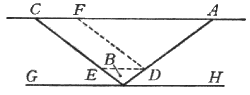
\includegraphics[width=6.25cm,height=2.38cm,keepaspectratio]{images/figura60.png} \end{center}
\end{center}

Si intenda pertanto che la discesa si sia svolta sul piano declive \emph{AB}, e che in séguito il moto continui riflesso su un altro piano acclive \emph{BC}; e, in primo luogo, i piani siano eguali ed elevati sull'orizzonte \emph{GH} con angoli [di inclinazione] eguali: già sappiamo che il mobile, che discende per \emph{AB} a partire dalla quiete in \emph{A}, acquista gradi di velocità secondo il crescere del tempo; inoltre [sappiamo] che il grado di velocità acquistato in \emph{B} è il massimo, e per sua natura immutabilmente impresso, rimosse beninteso le cause di nuova accelerazione o di ritardamento: vogliam dire, di accelerazione, se [il mobile] procede ancora sul prolungamento del medesimo piano; di ritardamento, allorché viene riflesso sul piano acclive \emph{BC}: ma sul piano orizzontale \emph{GH} il moto continuerebbe equabile all'infinito, col grado di velocità acquistato in \emph{B} nella discesa da \emph{A}; e la velocità sarebbe tale, che in un tempo eguale al tempo della discesa per \emph{AB} [il mobile] percorrerebbe sull'orizzonte uno spazio doppio del medesimo \emph{AB}. Immaginiamo ora che il medesimo mobile con il medesimo grado di velocità si muova equabilmente sul piano \emph{BC}, sì che, anche su questo, in un tempo eguale al tempo della discesa per \emph{AB}, percorrerebbe sul prolungamento di \emph{BC} uno spazio doppio del medesimo spazio \emph{AB}; intendiamo tuttavia che, non appena comincia a salire, per sua medesima natura gli sopravviene ciò stesso che gli accadde [nel muoversi] da \emph{A} sul piano \emph{AB}, cioè un moto di discesa a partire dalla quiete secondo medesimi gradi di accelerazione, in virtù dei quali, come già accadde sul piano \emph{AB}, in uno stesso tempo scenderebbe sul piano riflesso per uno spazio eguale a quello percorso in discesa su \emph{AB}: è manifesto che, per tale mescolanza di moto ascendente equabile e di moto discendente accelerato, il mobile verrà spinto sul piano \emph{BC} fino all'estremo \emph{C} secondo i medesimi gradi di velocità, che risulteranno eguali. Presi infatti due punti qualsiasi \emph{D} ed \emph{E}, ad eguale distanza dall'angolo \emph{B}, potremo ricavare che la discesa per \emph{DB} avverrà in un tempo eguale al tempo del moto riflesso per \emph{BE}. Tracciata la \emph{DF}, essa sarà parallela alla \emph{BC}; è noto infatti che il moto di discesa per \emph{AD} viene riflesso lungo la \emph{DF}: ora, se dopo \emph{D} il mobile si muovesse sull'orizzontale \emph{DE}, l'impeto in \emph{E} sarebbe eguale all'impeto in \emph{D}; dunque, da \emph{E} salirebbe fino in \emph{C}; dunque, il grado di velocità in \emph{D} è eguale al grado [di velocità] in \emph{E}.

Da ciò, pertanto, possiamo ragionevolmente asserire che, se ha luogo la discesa su un qualche piano inclinato e dopo di essa ha luogo la riflessione su un piano ascendente, il mobile, in virtù dell'impeto acquistato, salirà fino alla medesima altezza o elevazione dall'orizzonte; ad esempio,


\begin{center}
\begin{center} 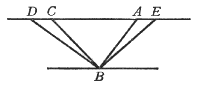
\includegraphics[width=5.00cm,height=2.20cm,keepaspectratio]{images/figura61.png} \end{center}
\end{center}

se la discesa si svolge lungo \emph{AB}, il mobile si muoverà sul piano riflesso \emph{BC} fino all'orizzontale \emph{ACD}, non soltanto se i piani avranno eguale inclinazione, ma anche se saranno di inclinazione diseguale, come il piano \emph{BD}: infatti, abbiamo prima assunto che i gradi di velocità, che si acquistano su piani diversamente inclinati, risultano eguali a condizione che sia eguale la elevazione di quegli stessi piani sull'orizzonte. Se infatti l'inclinazione dei piani \emph{EB} e \emph{BD} fosse la medesima, la discesa per \emph{EB} sarebbe in grado di spingere il mobile sul piano \emph{BD} fino al punto \emph{D}; ma tale spinta ha luogo in virtù dell'impeto di velocità acquistato nel punto \emph{B}, e in \emph{B} l'impeto è lo stesso, sia che il mobile scenda per \emph{AB}, sia che scenda per \emph{EB}; ne risulta allora che il mobile sarà spinto sul piano \emph{BD} dopo la discesa per \emph{AB} allo stesso modo che dopo la discesa per \emph{EB}. Accadrà però che il tempo della salita sul piano \emph{BD} sarà più lungo del tempo della salita sul piano \emph{BC}, siccome anche la discesa per \emph{EB} avviene in un tempo più lungo di quella per \emph{AB}; del resto, abbiamo già dimostrato che la proporzione dei tempi è eguale a quella delle lunghezze dei piani. Ci resta ora da investigare la proporzione tra gli spazi percorsi in tempi eguali su piani, che abbiano diverse inclinazioni, ma eguale elevazione, cioè che siano compresi entro le medesime parallele orizzontali. Ciò avviene secondo la seguente proporzione.

\textbf{TEOREMA 15. PROPOSIZIONE 24}


\begin{center}
\begin{center} 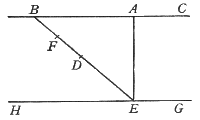
\includegraphics[width=5.00cm,height=3.00cm,keepaspectratio]{images/figura62.png} \end{center}
\end{center}

Siano dati, [nello spazio compreso] entro le medesime parallele orizzontali, una perpendicolare e un piano inclinato innalzato dall'estremo inferiore di essa: lo spazio, che il mobile dopo la caduta lungo la perpendicolare percorre sul piano ascendente in un tempo eguale al tempo della caduta, è maggiore della stessa perpendicolare, ma minore del doppio di essa.

\textbf{TEOREMA 16. PROPOSIZIONE 25}


\begin{center}
\begin{center} 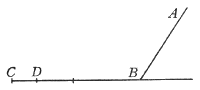
\includegraphics[width=5.00cm,height=2.25cm,keepaspectratio]{images/figura63.png} \end{center}
\end{center}

Se, dopo la caduta lungo un piano inclinato, il moto prosegue sul piano dell'orizzonte, il tempo della caduta lungo il piano inclinato starà al tempo del moto lungo un qualsiasi tratto dell'orizzonte, come il doppio della lunghezza del piano inclinato sta al tratto orizzontale preso.

\textbf{PROBLEMA 10. PROPOSIZIONE 26}


\begin{center}
\begin{center} 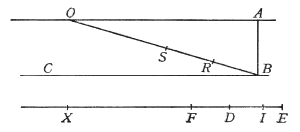
\includegraphics[width=7.50cm,height=3.30cm,keepaspectratio]{images/figura64.png} \end{center}
\end{center}

Data una perpendicolare [compresa] tra linee parallele orizzontali, e dato uno spazio maggiore della medesima perpendicolare, ma minore del doppio di essa, dall'estremo inferiore della perpendicolare innalzare, [nello spazio compreso] tra quelle medesime parallele, un piano tale che il mobile, se riflesso su questo piano dopo la discesa lungo la perpendicolare, percorra uno spazio eguale a quello dato, e in un tempo eguale al tempo della discesa lungo la perpendicolare.

\textbf{TEOREMA 17. PROPOSIZIONE 27}


\begin{center}
\begin{center} 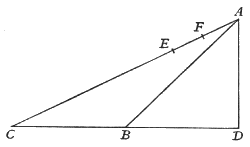
\includegraphics[width=6.25cm,height=3.68cm,keepaspectratio]{images/figura65.png} \end{center}
\end{center}

Se un mobile scende su piani diseguali, ma aventi la medesima elevazione, lo spazio, che viene percorso nella parte inferiore del piano più lungo in un tempo eguale a quello impiegato a percorrere l'intero piano più breve, è eguale allo spazio composto dello stesso piano più breve e di quel tratto rispetto al quale il medesimo piano più breve ha una proporzione pari a quella che il piano più lungo ha rispetto all'eccesso del più lungo sul più breve.

\textbf{PROBLEMA 11. PROPOSIZIONE 28}


\begin{center}
\begin{center} 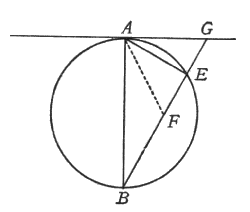
\includegraphics[width=6.25cm,height=5.30cm,keepaspectratio]{images/figura66.png} \end{center}
\end{center}

La linea orizzontale \emph{AG} sia tangente a un cerchio, e dal punto di contatto si conduca il diametro \emph{AB}; si considerino inoltre due corde qualsiasi \emph{AEB}: bisogna determinare la proporzione del tempo della caduta lungo \emph{AB} al tempo della discesa lungo ambedue le corde \emph{AEB}.

\textbf{TEOREMA 18. PROPOSIZIONE 29}\\ Sia dato uno spazio orizzontale qualsiasi, e dal suo estremo sia innalzata la perpendicolare, sulla quale si prenda un tratto eguale alla metà dello spazio orizzontale dato; il mobile, che scenda da tale altezza e sia deviato sul piano orizzontale, percorrerà lo spazio orizzontale e la perpendicolare, presi insieme, in più breve tempo di [quello che impiegherebbe a percorrere] un qualsiasi altro tratto della perpendicolare insieme al medesimo spazio orizzontale.

\textbf{TEOREMA 19. PROPOSIZIONE 30}\\ Se da un punto di una linea orizzontale scende una perpendicolare e da un altro punto, preso sulla medesima orizzontale, si deve condurre fino alla perpendicolare un piano inclinato, sul quale il mobile impieghi il tempo più breve per scendere fino alla perpendicolare; tale piano sarà quello che stacca dalla perpendicolare un tratto eguale alla distanza che intercorre tra il [secondo] punto preso sull'orizzontale e l'estremo della perpendicolare.

\textbf{TEOREMA 20. PROPOSIZIONE 31}


\begin{center}
\begin{center} 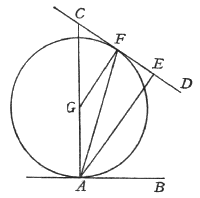
\includegraphics[width=5.00cm,height=4.95cm,keepaspectratio]{images/figura67.png} \end{center}
\end{center}

Se, tracciata una linea retta comunque inclinata sull'orizzontale, si conduce da un dato punto dell'orizzontale fino alla linea inclinata il piano, sul quale la discesa si svolge nel tempo più breve, tale piano sarà quello che divide a metà l'angolo compreso tra le due perpendicolari che, dal punto dato, vengano condotte, l'una alla linea orizzontale, l'altra alla linea inclinata.

\textbf{LEMMA}


\begin{center}
\begin{center} 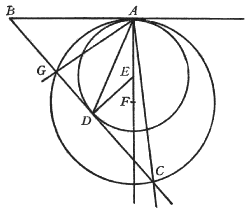
\includegraphics[width=6.25cm,height=5.48cm,keepaspectratio]{images/figura68.png} \end{center}
\end{center}

Date due circonferenze tangenti internamente l'una all'altra, se una retta qualsiasi è tangente alla circonferenza interna e interseca la circonferenza esterna, le tre linee condotte dal punto di contatto delle circonferenze ai tre punti della linea retta tangente - cioè al punto di contatto di essa con la circonferenza interna e ai due punti di intersezione di essa con la circonferenza esterna - formeranno angoli eguali [aventi per vertice] il punto di contatto delle circonferenze.

\textbf{TEOREMA 21. PROPOSIZIONE 32}\\ Se sull'orizzontale si prendono due punti e, a partire da uno di essi, si traccia una qualsiasi linea inclinata verso la parte dell'altro punto, e se a partire da quest'ultimo si conduce una linea retta, la quale incontri la predetta inclinata determinando su di essa un tratto eguale alla distanza fra i due punti dati sull'orizzontale, la caduta lungo questa retta si compirà più presto che non lungo qualsiasi altra retta condotta da quel medesimo punto fino a incontrare la medesima inclinata. Prese poi due rette qualsiasi, che formino con la retta data due angoli eguali da una parte e dall'altra, i tempi di caduta lungo di esse saranno eguali tra di loro.

\textbf{PROBLEMA 12. PROPOSIZIONE 33}\\ Dati una perpendicolare e un piano ad essa inclinato, che abbiano la medesima altezza e lo stesso estremo superiore, trovare lungo la perpendicolare, al di sopra dell'estremo in comune, un punto tale, che se da esso si lascia cadere un mobile, il quale venga poi fatto deviare sul piano inclinato, [quel mobile] percorra questo piano nello stesso tempo in cui percorrerebbe la perpendicolare a partire dalla quiete.

\textbf{PROBLEMA 13. PROPOSIZIONE 34}\\ Dati un piano inclinato e una perpendicolare, che abbiano il medesimo estremo superiore, trovare sul prolungamento della perpendicolare un punto più alto [dell'estremo comune], tale che un mobile, il quale cada da esso e sia deviato sul piano inclinato, li percorra entrambi in un tempo eguale a quello in cui percorrerebbe il solo piano inclinato [se partisse] dalla quiete nell'estremo superiore di questo.

\textbf{PROBLEMA 14. PROPOSIZIONE 35}\\ Data una perpendicolare e data una retta inclinata su di essa, determinare sull'inclinata un tratto, il quale da solo, [con movimento] a partire dalla quiete, sia percorso in un tempo eguale a quello impiegato a percorrere la medesima inclinata insieme alla perpendicolare.

\textbf{TEOREMA 22. PROPOSIZIONE 36}\\ Se in un cerchio, eretto sull'orizzonte, dal suo punto più basso si innalza un piano inclinato, il quale sottenda un arco non maggiore di un quadrante, e se dagli estremi di tale piano si conducono due altri piani inclinati a un qualsiasi punto dell'arco, la discesa lungo [il sistema di] questi due ultimi piani inclinati si compirà in minor tempo che lungo il solo primo piano inclinato, o che lungo uno soltanto di questi due ultimi piani, e precisamente l'inferiore.

\textbf{SCOLIO}


\begin{center}
\begin{center} 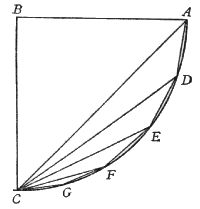
\includegraphics[width=5.00cm,height=5.23cm,keepaspectratio]{images/figura69.png} \end{center}
\end{center}

Da quanto si è dimostrato sembra si possa ricavare che il movimento più veloce da estremo ad estremo non avviene lungo la linea più breve, cioè la retta, ma lungo un arco di cerchio. Infatti, nel quadrante \emph{BAEC}, il cui lato \emph{BC} sia eretto sull'orizzonte, si divida l'arco \emph{AC} in un numero qualsiasi di parti eguali \emph{AD}, \emph{DE}, \emph{EF}, \emph{FG}, \emph{GC}; da \emph{C} si conducano le corde ai punti \emph{A}, \emph{D}, \emph{E}, \emph{F}, \emph{G}, e si traccino pure le corde \emph{AD}, \emph{DE}, \emph{EF}, \emph{FG}, \emph{G} \emph{C}: è manifesto che il movimento lungo [il sistema del]le due corde \emph{ADC} si compie più presto che lungo la sola \emph{AC}, o lungo \emph{DC} a partire dalla quiete in \emph{D}. Ma a partire dalla quiete in \emph{A}, \emph{DC} viene percorsa più presto di \emph{ADC}: ma lungo le due \emph{DEC} a partire dalla quiete in \emph{A}, è verisimile che la discesa si compia più presto che non lungo la sola \emph{CD}: dunque, la discesa lungo le tre corde \emph{ADEC} si compie più presto che non lungo le due \emph{ADC}. E similmente, dopo la discesa lungo \emph{ADE}, il movimento si svolge più presto lungo le due corde \emph{EFC} che non lungo la sola \emph{EC}; dunque, lungo le quattro corde \emph{ADEFC} il movimento si svolge più presto che non lungo le tre \emph{ADEC}. E infine, lungo le due corde \emph{FGC}, dopo la discesa lungo \emph{ADEF}, il movimento si compie più presto che non lungo la sola \emph{FC}; dunque, lungo le cinque corde \emph{ADEFGC} la discesa si svolge in un tempo ancora più breve che non lungo le quattro \emph{ADEFC}. Pertanto, quanto più, con poligoni inscritti [\emph{poligonali iscritte}] ci avviciniamo alla circonferenza, tanto più presto si compie il moto tra i due segnati estremi \emph{A} e \emph{C}.

Ciò che si è mostrato in un quadrante, accade anche in un arco di circonferenza minore di un quadrante; e identico è il ragionamento.

\textbf{PROBLEMA 15. PROPOSIZIONE 37}\\ Dati una perpendicolare e un piano inclinato, che abbiano la medesima elevazione, trovare sul piano inclinato un tratto, il quale sia eguale alla perpendicolare e venga percorso nello stesso tempo di quest'ultima.

\textbf{PROBLEMA 16. PROPOSIZIONE 38}\\ Dati due piani orizzontali intersecati da una perpendicolare, trovare su questa, in alto, un punto tale, che due mobili, i quali cadano da quel punto e vengano deviati sui piani orizzontali, percorrano su di questi, cioè sul piano orizzontale superiore e su quello inferiore, in tempi eguali a quelli della loro [rispettiva] caduta, spazi tali che abbiano tra loro una proporzione eguale a una qualsiasi proporzione data fra una [grandezza] minore e una maggiore.

\speaker{Sagr.} Parmi veramente che conceder si possa al nostro Accademico, che egli senza iattanza abbia nel principio di questo suo trattato potuto attribuirsi di arrecarci una nuova scienza intorno a un suggetto antichissimo. Ed il vedere con quanta facilità e chiarezza da un solo semplicissimo principio ei deduca le dimostrazioni di tante proposizioni, mi fa non poco maravigliare come tal materia sia passata intatta da Archimede, Apollonio, Euclide e tanti altri matematici e filosofi illustri, e massime che del moto si trovano scritti volumi grandi e molti.

\speaker{Salv.} Si vede un poco di fragmento d'Euclide intorno al moto, ma non vi si scorge vestigio che egli s'incaminasse all'investigazione della proporzione dell'accelerazione e delle sue diversità sopra le diverse inclinazioni. Tal che veramente si può dire, essersi non prima che ora aperta la porta ad una nuova contemplazione, piena di conclusioni infinite ed ammirande, le quali ne i tempi avenire potranno esercitare altri ingegni.

\speaker{Sagr.} Io veramente credo, che sì come quelle poche passioni (dirò per esempio) del cerchio, dimostrate nel terzo de' suoi Elementi da Euclide, sono l'ingresso ad innumerabili altre più recondite, così le prodotte e dimostrate in questo breve trattato, quando passasse nelle mani di altri ingegni specolativi, sarebbe strada ad altre ed altre più maravigliose; ed è credibile che così seguirebbe, mediante la nobiltà del soggetto sopra tutti gli altri naturali.

Lunga ed assai laboriosa giornata è stata questa d'oggi, nella quale ho gustato più delle semplici proposizioni che delle loro dimostrazioni, molte delle quali credo che, per ben capirle, mi porteranno via più d'un'ora per ciascheduna: studio che mi riserbo a farlo con quiete, lasciandomi V. S. il libro nelle mani, dopo che avremo veduto questa parte che resta intorno al moto de i proietti; che sarà, se così gli piace, nel seguente giorno.

\speaker{Salv.} Non mancherò d'esser con lei.

\textbf{Note:}

(1) Il brano in forma di dialogo tra le interlinee, che Galileo voleva inserire in questo punto, è stato scritto dal suo discepolo Vincenzo Viviani (Firenze 1622-1703). [\emph{nota per l'edizione elettronica Manuzio}]

(2) In realtà, avendo l'edizione U.T.E.T. omesso una dimostrazione, ci si riferisce qui all'ultima figura. [\emph{nota per l'edizione elettronica Manuzio}]


\vspace{1.5em}\begin{center}\large\itshape Finisce la terza Giornata\end{center}

\chapter*{Giornata Quarta\\{\normalsize\itshape Del Moto dei Proietti}}
\addcontentsline{toc}{chapter}{Giornata Quarta — Del Moto dei Proietti}
\markboth{Giornata Quarta}{Del Moto dei Proietti}
\speaker{Salv.} Attempo arriva ancora il Sig. Simplicio; però, senza interpor quiete, venghiamo al moto: ed ecco il testo del nostro Autore.


\section*{DEL MOTO DEI PROIETTI}
\addcontentsline{toc}{section}{Del Moto Dei Proietti}

Le proprietà che si presentano nel moto equabile, come pure nel moto naturalmente accelerato su piani di qualsiasi inclinazione, le abbiamo considerate sopra. Nella trattazione, che ora comincio, cercherò di presentare, e di stabilire sulla base di salde dimostrazioni, alcuni fenomeni notevoli e degni di essere conosciuti, che sono propri di un mobile, mentre si muove con moto composto di un duplice movimento, cioè di un movimento equabile e di uno naturalmente accelerato: tale appunto sembra essere quello che chiamiamo moto dei proietti; la generazione del quale così stabilisco.

Immagino di avere un mobile lanciato su un piano orizzontale, rimosso ogni impedimento: già sappiamo, per quello che abbiamo detto più diffusamente altrove, che il suo moto si svolgerà equabile e perpetuo sul medesimo piano, qualora questo si estenda all'infinito; se invece intendiamo [questo piano] limitato e posto in alto, il mobile, che immagino dotato di gravità, giunto all'estremo del piano e continuando la sua corsa, aggiungerà al precedente movimento equabile e indelebile quella propensione all'ingiù dovuta alla propria gravità: ne nasce un moto composto di un moto orizzontale equabile e di un moto \emph{deorsum} naturalmente accelerato, il quale [moto composto] chiamo proiezione. Ne dimostreremo parecchie proprietà: la prima delle quali sia [\emph{la seguente}].

\textbf{TEOREMA 1. PROPOSIZIONE 1}\\ Un proietto, mentre si muove di moto composto di un moto orizzontale equabile e di un moto \emph{deorsum} naturalmente accelerato, descrive nel suo movimento una linea semiparabolica.

\speaker{Sagr.} È forza, Sig. Salviati, in grazia di me, ed anco, credo io, del Sig. Simplicio, far qui un poco di pausa; avvenga che io non mi son tanto inoltrato nella geometria, che io abbia fatto studio in Apollonio, se non in quanto so ch'ei tratta di queste parabole e dell'altre sezzioni coniche, senza la cognizione delle quali e delle lor passioni non credo che intendersi possano le dimostrazioni di altre proposizioni a quelle aderenti. E perché già nella bella prima proposizione ci vien proposto dall'Autore, doversi dimostrare, la linea descritta dal proietto esser parabolica, mi vo imaginando che, non dovendosi trattar d'altro che di tali linee, sia assolutamente necessario avere una perfetta intelligenza, se non di tutte le passioni di tali figure dimostrate da Apollonio, almeno di quelle che per la presente scienza son necessarie.

\speaker{Salv.} V. S. si umilia molto, volendosi far nuovo di quelle cognizioni le quali non è gran tempo che ammesse come ben sapute, allora, dico, che nel trattato delle resistenze avemmo bisogno della notizia di certa proposizione d'Apollonio, sopra la quale ella non mosse difficoltà.

\speaker{Sagr.} Può essere o che io la sapessi per ventura o che io la supponessi per una volta tanto che ella mi bisognò in tutto quel trattato: ma qui, dove mi imagino d'avere a sentir tutte le dimostrazioni circa tali linee, non bisogna, come si dice, bever grosso, buttando via il tempo e la fatica.

\speaker{Simp.} E poi, rispetto a me, quando bene, come credo, il Sig. Sagredo fusse ben corredato di tutti i suoi bisogni, a me cominciano già a giugner come nuovi gli stessi primi termini; perché, se bene i nostri filosofi hanno trattata questa materia del moto de' proietti, non mi sovvien che si siano ristretti a definire quali siano le linee da quelli descritte, salvo che assai generalmente sian sempre linee curve, eccetto che nelle proiezzioni perpendicolari \emph{sursum}. Però, quando quel poco di geometria che io ho appreso da Euclide, da quel tempo in qua che noi avemmo altri discorsi, non sia bastante per rendermi capace delle cognizioni necessarie per l'intelligenza delle seguenti dimostrazioni, mi converrà contentarmi delle sole proposizioni credute, ma non sapute.

\speaker{Salv.} Anzi voglio io che le sappiate mercé dell'istesso Autor dell'opera, il quale, quando già mi concesse di veder questa sua fatica, perché io ancora in quella volta non aveva in pronto i libri di Apollonio, s'ingegnò di dimostrarmi due passioni principalissime di essa parabola, senza veruna altra precognizione, delle quali sole siamo bisognosi nel presente trattato: le quali son ben anco provate da Apollonio, ma dopo molte altre, che lungo sarebbe a vederle; ed io voglio che abbreviamo assai il viaggio, cavando la prima immediatamente dalla pura e semplice generazione di essa parabola, e da questa poi pure immediatamente la dimostrazione della seconda. Venendo dunque alla prima:


\begin{center}
\begin{center} 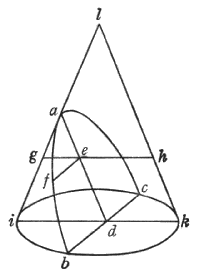
\includegraphics[width=5.00cm,height=6.90cm,keepaspectratio]{images/figura70.png} \end{center}
\end{center}

Intendasi il cono retto, la cui base sia il cerchio \emph{ibkc}, e vertice il punto \emph{l}, nel quale, segato con un piano parallelo al lato \emph{lk}, nasca la sezzione \emph{bac}, detta \emph{parabola}; la cui base \emph{bc} seghi ad angoli retti il diametro \emph{ik} del cerchio \emph{ibkc}, e sia l'asse della parabola \emph{ad} parallelo al lato \emph{lk}; e preso qualsivoglia punto \emph{f} nella linea \emph{bfa}, tirisi la retta \emph{fe} parallela alla \emph{bd}: dico che il quadrato della \emph{bd} al quadrato della \emph{fe} ha la medesima proporzione che l'asse \emph{da} alla parte \emph{ae}. Per il punto \emph{e} intendasi passare un piano parallelo al cerchio \emph{ibkc}, il quale farà nel cono una sezzione circolare, il cui diametro sia la linea \emph{geh}: e perché sopra il diametro \emph{ik} del cerchio \emph{ibk} la \emph{bd} è perpendicolare, sarà il quadrato della \emph{bd} eguale al rettangolo fatto dalle parti \emph{id}, \emph{dk}; e parimente nel cerchio superiore, che s'intende passare per i punti \emph{g}, \emph{f}, \emph{h}, il quadrato della linea \emph{fe} è eguale al rettangolo delle parti \emph{geh}; adunque il quadrato della \emph{bd} al quadrato della \emph{fe} ha la medesima proporzione che il rettangolo \emph{idk} al rettangolo \emph{geh}. E perché la linea \emph{ed} è parallela alla \emph{hk}, sarà la \emph{eh} eguale alla \emph{dk}, che pur son parallele: e però il rettangolo \emph{idk} al rettangolo \emph{geh} arà la medesima proporzione che la \emph{id} alla \emph{ge}, cioè che la \emph{da} alla \emph{ae}: adunque il rettangolo \emph{idk} al rettangolo \emph{geh}, cioè il quadrato \emph{bd} al quadrato \emph{fe}, ha la medesima proporzione che l'asse \emph{da} alla parte \emph{ae}: che bisognava dimostrare.

L'altra proposizione, pur necessaria al presente trattato, così faremo manifesta.


\begin{center}
\begin{center} 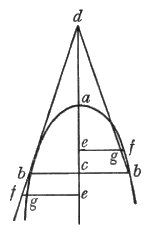
\includegraphics[width=3.75cm,height=5.83cm,keepaspectratio]{images/figura71.png} \end{center}
\end{center}

Segniamo la parabola, della quale sia prolungato fuori l'asse \emph{ca} in \emph{d}, e preso qualsivoglia punto \emph{b}, per esso intendasi prodotta la linea \emph{bc}, parallela alla base di essa parabola; e posta la \emph{da} eguale alla parte dell'asse \emph{ca}, dico che la retta tirata per i punti \emph{d}, \emph{b} non cade dentro alla parabola, ma fuori, sì che solamente la tocca nell'istesso punto \emph{b}. Imperò che, se è possibile, caschi dentro, segandola sopra, o, prolungata, segandola sotto, ed in essa sia preso qualsivoglia punto \emph{g}, per il quale passi la retta \emph{fge}. E perché il quadrato \emph{fe} è maggiore del quadrato \emph{ge}, maggior proporzione avrà esso quadrato \emph{fe} al quadrato \emph{bc} che 'l quadrato \emph{ge} al medesimo \emph{bc}; e perché, per la precedente, il quadrato \emph{fe} al quadrato \emph{bc} sta come la \emph{ea} alla \emph{ac}, adunque maggior proporzione ha la \emph{ea} alla \emph{ac} che 'l quadrato \emph{ge} al quadrato \emph{bc}, cioè che 'l quadrato \emph{ed} al quadrato \emph{dc} (essendo che nel triangolo \emph{dge} come la \emph{ge} alla parallela \emph{bc}, così sta \emph{ed} a \emph{dc}): ma la linea \emph{ea} alla \emph{ac}, cioè alla \emph{ad}, ha la medesima proporzione che 4 rettangoli \emph{ead} a 4 quadrati di \emph{ad}, cioè al quadrato \emph{cd} (che è eguale a 4 quadrati di \emph{ad}): adunque 4 rettangoli \emph{ead} al quadrato \emph{cd} aranno maggior proporzione che il quadrato \emph{ed} al quadrato \emph{dc}: adunque 4 rettangoli \emph{ead} saranno maggiori del quadrato \emph{ed}: il che è falso, perché son minori; imperò che le parti \emph{ea}, \emph{ad} della linea \emph{ed} non sono eguali. Adunque la linea \emph{db} tocca la parabola in \emph{b}, e non la sega: il che si doveva dimostrare.

\speaker{Simp.} Voi procedete nelle vostre dimostrazioni troppo alla grande, ed andate sempre, per quanto mi pare, supponendo che tutte le proposizioni di Euclide mi siano così familiari e pronte, come gli stessi primi assiomi, il che non è. E pur ora l'uscirmi addosso, che 4 rettangoli \emph{ead} son minori del quadrato \emph{de}, perché le parti \emph{ea}, \emph{ad} della linea \emph{ed} non sono equali, non mi quieta, ma mi lascia sospeso.

\speaker{Salv.} Veramente tutti i matematici non vulgari suppongono che il lettore abbia prontissimi al meno gli Elementi di Euclide: e qui, per supplire al vostro bisogno, basterà ricordarvi una proposizione del secondo, nella quale si dimostra, che quando una linea è segata in parti eguali ed in diseguali, il rettangolo delle parti diseguali è minore del rettangolo delle parti eguali (cioè del quadrato della metà) quanto è il quadrato della linea compresa tra i segamenti; onde è manifesto che il quadrato di tutta, il quale contiene 4 quadrati della metà, è maggiore di 4 rettangoli delle parti diseguali. Ora, di queste due proposizioni dimostrate, prese da gli elementi conici, conviene che tenghiamo memoria per l'intelligenza delle cose seguenti nel presente trattato: ché di queste sole, e non di più, si serve l'Autore. Ora possiamo ripigliare il testo, per vedere in qual maniera ei vien dimostrando la sua prima proposizione, dove egli intende di provarci la linea descritta dal mobile grave, che mentre ci descende con moto composto dell'equabile orizontale e del naturale descendente, sia una semiparabola.


\begin{center}
\begin{center} 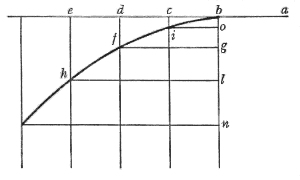
\includegraphics[width=7.50cm,height=4.50cm,keepaspectratio]{images/figura72.png} \end{center}
\end{center}

Si intenda la linea orizzontale ossia il piano \emph{ab} posto in alto, e un mobile si muova su di esso da \emph{a} in \emph{b} di moto equabile; mancando ora il sostegno del piano in \emph{b}, sopravvenga al medesimo mobile, per la propria gravità, un moto naturale \emph{deorsum} secondo la perpendicolare \emph{bn}. Si intenda inoltre che la linea \emph{be}, la quale prosegue il piano \emph{ab} per diritto, rappresenti lo scorrere del tempo, ossia [ne costituisca] la misura, e su di essa si segnino ad arbitrio un numero qualsiasi di porzioni di tempo eguali, \emph{bc}, \emph{cd}, \emph{de}; inoltre dai punti \emph{b}, \emph{c}, \emph{d}, \emph{e} si intendano condotte linee equidistanti dalla perpendicolare \emph{bn}: sulla prima di esse si prenda una parte qualsiasi \emph{ci}; sulla [linea] successiva se ne prenda una quattro volte maggiore, \emph{df}; [sulla terza,] una nove volte maggiore, \emph{eh}; e così di séguito sulle altre linee secondo la proporzione dei quadrati delle [porzioni di tempo] \emph{cb}, \emph{db}, \emph{eb}, o vogliam dire in duplicata proporzione delle medesime. Se poi intendiamo che al mobile, il quale si muove oltre \emph{b} verso \emph{c} con moto equabile, si aggiunga un movimento di discesa perpendicolare secondo la quantità \emph{ci}, nel tempo \emph{bc} [esso mobile] si troverà situato nell'estremo \emph{i}. Ma continuando a muoversi, nel tempo \emph{db}, cioè [in un tempo] doppio di \emph{bc}, sarà disceso per uno spazio quattro volte maggiore del primo spazio \emph{ci}; abbiamo infatti dimostrato nel primo trattato, che gli spazi percorsi da un grave, con moto naturalmente accelerato, sono in duplicata proporzione dei tempi: e parimenti, il successivo spazio \emph{eh}, percorso nel tempo \emph{be}, sarà nove [volte maggiore del primo spazio]: sì che risulterà manifesto che gli spazi \emph{eh}, \emph{df}, \emph{ci} stanno tra di loro come i quadrati delle linee \emph{eb}, \emph{db}, \emph{cb}. Si conducano ora dai punti \emph{i}, \emph{f}, \emph{h} le rette \emph{io}, \emph{fg}, \emph{hl}, equidistanti dalla medesima \emph{eb}: le linee \emph{hl}, \emph{fg}, \emph{io} saranno eguali, ad una ad una, alle linee \emph{eb}, \emph{db}, \emph{cb}; e così pure le linee \emph{bo}, \emph{bg}, \emph{bl} saranno eguali alle linee \emph{ci}, \emph{df}, \emph{eh}; inoltre il quadrato di \emph{hl} starà al quadrato di \emph{fg} come la linea \emph{lb} sta alla \emph{bg}, e il quadrato di \emph{fg} starà al quadrato di \emph{io} come \emph{gb} sta a \emph{bo}; dunque, i punti \emph{i}, \emph{f}, \emph{h} si trovano su un unica e medesima linea parabolica. Similmente si dimostrerà che, preso un numero qualsiasi di particole di tempo eguali di qualunque grandezza, i punti, che il mobile mosso di un simile moto composto occuperà in quei tempi, si troveranno su una medesima linea parabolica. È dunque manifesto quello che ci eravamo proposti.

\speaker{Salv.} Questa conclusione si raccoglie dal converso della prima delle due proposizioni poste di sopra. Imperò che, descritta, per esempio, la parabola per li punti \emph{b}, \emph{h}, se alcuno delli 2 \emph{f}, \emph{i} non fusse nella descritta linea parabolica, sarebbe dentro o fuori, e, per conseguenza, la linea \emph{fg} sarebbe o minore o maggiore di quella che andasse a terminare nella linea parabolica; onde il quadrato della \emph{hl} non al quadrato della \emph{fg}, ma ad altro maggiore o minore, arebbe la medesima proporzione che ha la linea \emph{lb} alla \emph{bg}: ma la ha al quadrato della \emph{fg}: adunque il punto \emph{f} è nella parabolica: e così tutti gli altri, etc.

\speaker{Sagr.} Non si può negare che il discorso sia nuovo, ingegnoso e concludente, argomentando \emph{ex suppositione}, supponendo cioè che il moto traversale si mantenga sempre equabile, e che il naturale \emph{deorsum} parimente mantenga il suo tenore, d'andarsi sempre accelerando secondo la proporzion duplicata de i tempi, e che tali moti e loro velocità, nel mescolarsi, non si alterino perturbino ed impedischino, sì che finalmente la linea del proietto non vadia, nella continuazion del moto, a degenerare in un'altra spezie: cosa che mi si rappresenta come impossibile. Imperò che, stante che l'asse della parabola nostra, secondo 'l quale noi supponghiamo farsi il moto naturale de i gravi, essendo perpendicolare all'orizonte, va a terminar nel centro della terra; ed essendo che la linea parabolica si va sempre slargando dal suo asse; niun proietto andrebbe già mai a terminar nel centro, o, se vi andrebbe, come par necessario, la linea del proietto tralignerebbe in altra, diversissima dalla parabolica.

\speaker{Simp.} Io a queste difficoltà ne aggiungo dell'altre: una delle quali è, che noi supponghiamo che il piano orizontale, il quale non sia né acclive né declive, sia una linea retta, quasi che una simil linea sia in tutte le sue parti egualmente distante dal centro, il che non è vero; perché, partendosi dal suo mezo, va verso le estremità sempre più e più allontanandosi dal centro, e però ascendendo sempre; il che si tira in conseguenza, essere impossibile che il moto si perpetui, anzi che né pur per qualche spazio si mantenga equabile, ma ben sempre vadia languendo. In oltre, è, per mio credere, impossibile lo schivar l'impedimento del mezo, sì che non levi l'equabilità del moto trasversale e la regola dell'accelerazione ne i gravi cadenti. Dalle quali tutte difficoltà si rende molto improbabile che le cose dimostrate con tali supposizioni incostanti possano poi nelle praticate esperienze verificarsi.

\speaker{Salv.} Tutte le promosse difficoltà e instanze son tanto ben fondate, che stimo essere impossibile il rimuoverle, ed io, per me, le ammetto tutte, come anco credo che il nostro Autore esso ancora le ammetterebbe; e concedo che le conclusioni così in astratto dimostrate si alterino in concreto, e si falsifichino a segno tale, che né il moto trasversale sia equabile, né l'accelerazione del naturale sia con la proporzion supposta, né la linea del proietto sia parabolica, etc.: ma ben, all'incontro, domando che elle non contendano al nostro Autor medesimo quello che altri grandissimi uomini hanno supposto, ancor che falso. E la sola autorità d'Archimede può quietare ogn'uno, il quale, nelle sue Mecaniche e nella prima Quadratura della parabola, piglia come principio vero, l'ago della bilancia o stadera essere una linea retta in ogni suo punto equalmente distante dal centro commune de i gravi, e le corde alle quali sono appesi i gravi esser tra di loro parallele: la qual licenza viene da alcuni scusata, perché nelle nostre pratiche gli strumenti nostri e le distanze le quali vengono da noi adoperate, son così piccole in comparazione della nostra gran lontananza dal centro del globo terrestre, che ben possiamo prendere un minuto di un grado del cerchio massimo come se fusse una linea retta, e due perpendicoli che da i suoi estremi pendessero, come se fussero paralleli. Che quando nelle opere praticali si avesse a tener conto di simili minuzie, bisognerebbe cominciare a riprendere gli architetti, li quali col perpendicolo suppongono d'alzar le altissime torri tra linee equidistanti. Aggiungo qui, che noi possiamo dire che Archimede e gli altri supposero nelle loro contemplazioni, esser costituiti per infinita lontananza remoti dal centro, nel qual caso i loro assunti non erano falsi, e che però concludevano con assoluta dimostrazione. Quando poi noi vogliamo praticar in distanza terminata le conclusioni dimostrate col suppor lontananza immensa, doviamo diffalcar dal vero dimostrato quello che importa il non esser la nostra lontananza dal centro realmente infinita, ma ben tale che domandar si può immensa in comparazione della piccolezza de gli artificii praticati da noi: il maggior de i quali sarà il tiro de i proietti, e di questi quello solamente dell'artiglierie, il quale, per grande che sia, non passerà 4 miglia di quelle delle quali noi siamo lontani dal centro quasi altrettante migliara; ed andando questi a terminar nella superficie del globo terrestre, ben potranno solo insensibilmente alterar quella figura parabolica, la quale si concede che sommamente si trasformerebbe nell'andare a terminar nel centro.

Quanto poi al perturbamento procedente dall'impedimento del mezo, questo è più considerabile, e, per la sua tanto moltiplice varietà, incapace di poter sotto regole ferme esser compreso e datone scienza; atteso che, se noi metteremo in considerazione il solo impedimento che arreca l'aria a i moti considerati da noi, questo si troverà perturbargli tutti, e perturbargli in modi infiniti, secondo che in infiniti modi si variano le figure, le gravità e le velocità de i mobili. Imperò che, quanto alla velocità, secondo che questa sarà maggiore, maggiore sarà il contrasto fattogli dall'aria; la quale anco impedirà più i mobili secondo che saranno men gravi: talché, se bene il grave descendente dovrebbe andare accelerandosi in duplicata proporzione della durazion del suo moto, tuttavia, per gravissimo che fusse il mobile, nel venir da grandissime altezze sarà tale l'impedimento dell'aria, che gli torrà il poter crescere più la sua velocità, e lo ridurrà ad un moto uniforme ed equabile; e questa adequazione tanto più presto ed in minori altezze si otterrà, quanto il mobile sarà men grave. Quel moto anco che nel piano orizontale, rimossi tutti gli altri ostacoli, devrebbe essere equabile e perpetuo, verrà dall'impedimento dell'aria alterato, e finalmente fermato: e qui ancora tanto più presto, quanto il mobile sarà più leggiero. De i quali accidenti di gravità, di velocità, ed anco di figura, come variabili in modi infiniti, non si può dar ferma scienza: e però, per poter scientificamente trattar cotal materia, bisogna astrar da essi, e ritrovate e dimostrate le conclusioni astratte da gl'impedimenti, servircene, nel praticarle, con quelle limitazioni che l'esperienza ci verrà insegnando. E non però piccolo sarà l'utile, perché le materie e lor figure saranno elette le men soggette a gl'impedimenti del mezo, quali sono le gravissime e le rotonde, e gli spazii e le velocità per lo più non saranno sì grandi, che le loro esorbitanze non possano con facil tara esser ridotte a segno; anzi pure ne i proietti praticabili da noi, che siano di materie gravi e di figura rotonda, ed anco di materie men gravi e di figura cilindrica, come frecce, lanciati con frombe o archi, insensibile sarà del tutto lo svario del lor moto dall'esatta figura parabolica. Anzi (e voglio pigliarmi alquanto più di licenza) che ne gli artifizii da noi praticabili la piccolezza loro renda pochissimo notabili gli esterni ed accidentarii impedimenti, tra i quali quello del mezo è il più considerabile, vi posso io con due esperienze far manifesto. Io farò considerazione sopra i movimenti fatti per l'aria, ché tali son principalmente quelli de i quali noi parliamo; contro i quali essa aria in due maniere esercita la sua forza: l'una è coll'impedir più i mobili men gravi che i gravissimi; l'altra è nel contrastar più alla velocità maggiore che alla minore dell'istesso mobile. Quanto al primo, il mostrarci l'esperienza che due palle di grandezza eguali, ma di peso l'una 10 o 12 volte più grave dell'altra, quali sarebbero, per esempio, una di piombo e l'altra di rovere, scendendo dall'altezza di 150 o 200 braccia, con pochissimo differente velocità arrivano in terra, ci rende sicuri che l'impedimento e ritardamento dell'aria in amendue è poco: che se la palla di piombo, partendosi nell'istesso momento da alto con l'altra di legno, poco fusse ritardata, e questa molto, per assai notabile spazio devrebbe il piombo, nell'arrivare in terra, lasciarsi a dietro il legno, mentre è 10 volte più grave; il che tutta via non accade, anzi la sua anticipazione non sarà né anco la centesima parte di tutta l'altezza; e tra una palla di piombo ed una di pietra, che di quella pesasse la terza parte o la metà, appena sarebbe osservabile la differenza del tempo delle lor giunte in terra. Ora, perché l'impeto che acquista una palla di piombo nel cadere da un'altezza di 200 braccia (il quale è tanto, che continuandolo in moto equabile scorrerebbe braccia 400 in tanto tempo quanto fu quello della sua scesa) è assai considerabile rispetto alle velocità che noi con archi o altre machine conferiamo a i nostri proietti (trattone gl'impeti dependenti dal fuoco), possiamo senza errore notabile concludere e reputar come assolutamente vere le proposizioni che si dimostreranno senza il riguardo dell'alterazion del mezo. Circa poi all'altra parte, che è di mostrare, l'impedimento che l'istesso mobile riceve dall'aria, mentre egli con gran velocità si muove, non esser grandemente maggiore di quello che gli contrasta nel muoversi lentamente, ferma certezza ce ne porge la seguente esperienza. Sospendansi da due fili egualmente lunghi, e di lunghezza di 4 o 5 braccia, due palle di piombo eguali, e attaccati i detti fili in alto, si rimuovano amendue le palle dallo stato perpendicolare; ma l'una si allontani per 80 o più gradi, e l'altra non più che 4 o 5: sì che, lasciate in libertà, l'una scenda e, trapassando il perpendicolo, descrive archi grandissimi di 160, 150, 140 gradi, etc., diminuendogli a poco a poco; ma l'altra, scorrendo liberamente, passi archi piccoli di 10, 8, 6 etc., diminuendogli essa ancora a poco a poco: qui primieramente dico, che in tanto tempo passerà la prima li suoi gradi 180, 160 etc., in quanto l'altra li suoi 10, 8 etc. Dal che si fa manifesto, che la velocità della prima palla sarà 16 e 18 volte maggiore della velocità della seconda; sì che, quando la velocità maggiore più dovesse essere impedita dall'aria che la minore, più rade devriano esser le vibrazioni ne gli archi grandissimi di 180 e 160 gradi etc., che ne i piccolissimi di 10, 8, 4, ed anco di 2 e di 1: ma a questo repugna l'esperienza; imperò che se due compagni si metteranno a numerare le vibrazioni, l'uno le grandissime e l'altro le piccolissime, vedranno che ne numereranno non pur le decine, ma le centinaia ancora, senza discordar d'una sola, anzi d'un sol punto. E questa osservazione ci assicura congiuntamente delle 2 proposizioni, cioè che le massime e le minime vibrazioni si fanno tutte a una a una sotto tempi eguali, e che l'impedimento e ritardamento dell'aria non opera più ne i moti velocissimi che ne i tardissimi; contro a quello che pur dianzi pareva che noi ancora comunemente giudicassimo.

\speaker{Sagr.} Anzi, perché non si può negare che l'aria impedisca questi e quelli, poi che e questi e quelli vanno languendo e finalmente finiscono, convien dire che tali ritardamenti si facciano con la medesima proporzione nell'una e nell'altra operazione. Ma che? l'avere a far maggior resistenza una volta che un'altra, da che altro proced'egli fuor che dall'esser assalito una volta con impeto e velocità maggiore, ed un'altra con minore? E se questo è, la quantità medesima della velocità del mobile è cagione ed insieme misura della quantità della resistenza. Adunque tutti i moti, siano tardi o veloci, son ritardati e impediti con l'istessa proporzione: notizia, par a me, non disprezzabile.

\speaker{Salv.} Possiam per tanto anco in questo secondo caso concludere, che le fallacie nelle conclusioni le quali astraendo da gli accidenti esterni si dimostreranno, siano ne gli artifizii nostri di piccola considerazione, rispetto a i moti di gran velocità, de i quali per lo più si tratta, ed alle distanze, che non sono se non piccolissime in relazione alla grandezza del semidiametro e de i cerchi massimi del globo terrestre.

\speaker{Simp.} Io volentieri sentirei la cagione per la quale V. S. sequestra i proietti dall'impeto del fuoco, cioè, come credo, dalla forza della polvere, da gli altri proietti con frombe archi o balestre, circa 'l non essere nell'istesso modo soggetti all'alterazione ed impedimento dell'aria.

\speaker{Salv.} Muovemi l'eccessiva e, per via di dire, furia soprannaturale con la quale tali proietti vengono cacciati; ché bene anco fuora d'iperbole mi par che la velocità con la quale vien cacciata la palla fuori d'un moschetto o d'una artiglieria, si possa chiamar sopranaturale. Imperò che, scendendo naturalmente per l'aria da qualche altezza immensa una tal palla, la velocità sua, mercé del contrasto dell'aria, non si andrà accrescendo perpetuamente: ma quello che ne i cadenti poco gravi si vede in non molto spazio accadere, dico di ridursi finalmente a un moto equabile, accaderà ancora, dopo la scesa di qualche migliara di braccia, in una palla di ferro o di piombo; e questa terminata ed ultima velocità si può dire esser la massima che naturalmente può ottener tal grave per aria: la qual velocità io reputo assai minor di quella che alla medesima palla viene impressa dalla polvere accesa. Del che una assai acconcia esperienza ci può render cauti. Sparisi da un'altezza di cento o più braccia un archibuso con palla di piombo all'in giù perpendicolarmente sopra un pavimento di pietra, e col medesimo si tiri contro una simil pietra in distanza d'un braccio o 2, e veggasi poi qual delle 2 palle si trovi esser più ammaccata: imperò che, se la venuta da alto si troverà meno schiacciata dell'altra, sarà segno che l'aria gli avrà impedita e diminuita la velocità conferitagli dal fuoco nel principio del moto, e che, per conseguenza, una tanta velocità non gli permetterebbe l'aria che ella guadagnasse già mai venendo da quanto si voglia subblime altezza; ché quando la velocità impressagli dal fuoco non eccedesse quella che per se stessa, naturalmente scendendo, potesse acquistare, la botta all'ingiù devrebbe più tosto esser più valida che meno. Io non ho fatto tale esperienza, ma inclino a credere che una palla d'archibuso o d'artiglieria, cadendo da un'altezza quanto si voglia grande, non farà quella percossa che ella fa in una muraglia in lontananza di poche braccia, cioè di così poche, che 'l breve sdrucito, o vogliam dire scissura, da farsi nell'aria non basti a levar l'eccesso della furia sopranaturale impressagli dal fuoco. Questo soverchio impeto di simili tiri sforzati può cagionar qualche deformità nella linea del proietto, facendo 'l principio della parabola meno inclinato e curvo del fine; ma questo, poco o niente può esser di progiudizio al nostro Autore nelle praticali operazioni: tra le quali principale è la composizione d'una tavola per i tiri che dicono di volata, la quale contenga le lontananze delle cadute delle palle tirate secondo tutte le diverse elevazioni; e perché tali proiezzioni si fanno con mortari, e con non molta carica, in questi non essendo sopranaturale l'impeto, i tiri segnano le lor linee assai esattamente.

Ma in tanto procediamo avanti nel trattato, dove l'Autore ci vuole introdurre alla contemplazione ed investigazione dell'impeto del mobile, mentre si muove con moto composto di due; e prima, del composto di due equabili, l'uno orizontale e l'altro perpendicolare.

\textbf{TEOREMA 2. PROPOSIZIONE 2}\\ Se un mobile si muove con moto composto di due equabili, l'uno orizzontale e l'altro perpendicolare, l'impeto o momento del movimento composto da ambedue sarà in potenza eguale ai due momenti dei primi moti.


\begin{center}
\begin{center} 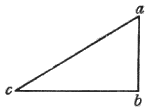
\includegraphics[width=3.75cm,height=2.75cm,keepaspectratio]{images/figura73.png} \end{center}
\end{center}

Un mobile, infatti, si muova equabilmente con un movimento duplice, e al movimento perpendicolare corrisponda lo spazio \emph{ab}, mentre al movimento orizzontale compiuto in un egual tempo corrisponda lo spazio \emph{bc}. Allora, poiché gli spazi \emph{ab} e \emph{bc} vengono percorsi nel medesimo tempo con moti equabili, i momenti di tali moti staranno tra di loro come le medesime \emph{ab} e \emph{bc}: ma il mobile, che si muove secondo questi due movimenti, descrive la diagonale \emph{ac}; il momento della sua velocità sarà dunque [rappresentato da] \emph{ac}. Ma \emph{ac} è eguale in potenza alle medesime \emph{ab} e \emph{bc}; dunque, il momento composto dai due momenti \emph{ab} e \emph{bc} sarà, soltanto in potenza, eguale a questi, presi insieme: che è quello che dovevamo mostrare.

\speaker{Simp.} È necessario levarmi un poco di scrupolo che qui mi nasce, parendomi che questo, che ora si conclude, repugni ad un'altra proposizione del trattato passato, nella quale si affermava, l'impeto del mobile venente dall'\emph{a} in \emph{b} essere eguale al venente dell'\emph{a} in \emph{c}; ed ora si conclude, l'impeto in \emph{c} esser maggiore che in \emph{b}.

\speaker{Salv.} Le proposizioni, Sig. Simplicio, sono amendue vere, ma molto diverse tra di loro. Qui si parla d'un sol mobile, mosso d'un sol moto, ma composto di due, amendue equabili; e là si parla di 2 mobili, mossi di moti naturalmente accelerati, uno per la perpendicolare \emph{ab}, e l'altro per l'inclinata \emph{ac}. In oltre, i tempi quivi non si suppongono eguali, ma il tempo per l'inclinata \emph{ac} è maggiore del tempo per la perpendicolare \emph{ab}; ma nel moto del quale si parla al presente, i moti per le \emph{ab}, \emph{bc}, \emph{ac} s'intendono equabili e fatti nell'istesso tempo.

\speaker{Simp.} Mi scusino, e seguano avanti, ché resto acquietato.

\speaker{Salv.} Séguita l'Autore per incaminarci a intender quel che accaggia intorno all'impeto d'un mobile mosso pur d'un moto composto di 2, uno cioè orizontale ed equabile, e l'altro perpendicolare ma naturalmente accelerato, de i quali finalmente è composto il moto del proietto e si descrive la linea parabolica, in ciaschedun punto della quale si cerca di determinare quanto sia l'impeto del proietto. Per la cui intelligenza ci dimostra l'Autore il modo, o vogliàn dir metodo, di regolare e misurar cotale impeto sopra l'istessa linea nella quale si fa il moto del grave descendente con moto naturalmente accelerato, partendosi dalla quiete, dicendo:

\textbf{TEOREMA 3. PROPOSIZIONE 3}


\begin{center}
\begin{center} 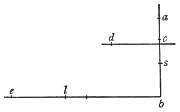
\includegraphics[width=4.50cm,height=2.80cm,keepaspectratio]{images/figura74.png} \end{center}
\end{center}

Il moto si svolga lungo la linea \emph{ab} a partire dalla quiete in \emph{a}, e su tale linea si prenda un qualsiasi punto \emph{c}; si ponga inoltre che la \emph{ac} sia il tempo, ossia la misura del tempo, della stessa caduta lungo lo spazio \emph{ac}, e che essa sia anche la misura dell'impeto o del momento acquistato nel punto \emph{c} in virtù della discesa \emph{ac}. Si prenda ora, sulla medesima linea \emph{ab}, un qualsiasi altro punto, come ad esempio \emph{b}: bisogna determinare l'impeto, acquistato in questo punto da un mobile che scenda per \emph{ab}, in proporzione all'impeto che aveva raggiunto in \emph{c}, a misura del quale si è posta la \emph{ac}. Si ponga \emph{as} media proporzionale tra \emph{ba} e \emph{ac}: dimostreremo che l'impeto in \emph{b} sta all'impeto in \emph{c} come la linea \emph{sa} sta alla \emph{ac}. Si prendano le orizzontali \emph{cd}, doppia della [linea] \emph{ac}, e \emph{be}, doppia della \emph{ba}: sappiamo, per le antecedenti dimostrazioni, che il mobile, il quale cada lungo \emph{ac}, sia deviato sull'orizzontale \emph{cd} e si muova di moto equabile secondo l'impeto acquistato in \emph{c}, percorre lo spazio \emph{cd} in un tempo eguale a quello impiegato a percorrere lo spazio \emph{ac} di moto accelerato; e similmente [sappiamo] che \emph{be} viene percorso nello stesso tempo di \emph{ab}: ma il tempo della discesa \emph{ab} è \emph{as}: dunque, la orizzontale \emph{be} viene percorsa nel tempo \emph{as}. Si faccia che, come il tempo \emph{sa} sta al tempo \emph{ac}, così \emph{eb} stia a \emph{bl}; essendo il moto lungo \emph{be} uniforme, lo spazio \emph{bl} verrà percorso nel tempo \emph{ac} secondo il momento di velocità [acquistato] in \emph{b}: ma nel medesimo tempo \emph{ac} viene percorso lo spazio \emph{cd} secondo il momento di velocità [acquistato] in \emph{c}; inoltre i momenti di velocità stanno tra di loro come gli spazi, che siano percorsi in tempi eguali con quegli stessi momenti di velocità: dunque, il momento di velocità in \emph{c} sta al momento di velocità in \emph{b}, come \emph{dc} sta a \emph{bl}. Ma poiché, come \emph{dc} sta a \emph{be}, così la metà dell'una sta alla metà dell'altra, cioè \emph{ca} ad \emph{ab}; e poiché, come \emph{eb} sta a \emph{bl}, così \emph{ba} sta ad \emph{as}; dunque, \emph{ex aequali}, come \emph{dc} sta a \emph{bl}, così \emph{ca} sta ad \emph{as}: cioè, come il momento di velocità in \emph{c} sta al momento di velocità in \emph{b}, così \emph{ca} sta ad \emph{as}, cioè, il tempo per \emph{ca} sta al tempo per \emph{ab}.

È pertanto chiaro il modo di misurare l'impeto o momento di velocità sulla linea lungo la quale si svolge il movimento di discesa; impeto che, come appunto abbiamo posto aumenta in proporzione al tempo.

Ma qui, prima di procedere oltre, bisogna premettere il seguente avvertimento: poiché il nostro discorso verterà intorno al moto composto di un moto orizzontale equabile e di un moto \emph{deorsum} naturalmente accelerato (da tale mescolanza, infatti, risulta composta e descritta la linea del proietto, cioè la parabola), ci troviamo nella necessità di determinare una misura comune, secondo la quale si possa misurare la velocità, l'impeto, ossia il momento di ambedue i moti; poiché nel moto equabile innumerevoli sono i gradi di velocità, ma di essi uno solo, e non uno qualsiasi a caso, deve essere correlato e congiunto al grado di velocità acquistato nel moto naturalmente accelerato, non ho potuto escogitare alcun altro modo più facile per sceglierlo e determinarlo, che assumendone un altro del medesimo genere. Ma per spiegarmi più chiaramente,


\begin{center}
\begin{center} 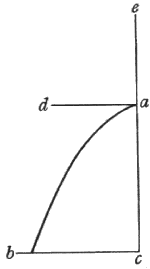
\includegraphics[width=3.75cm,height=6.73cm,keepaspectratio]{images/figura75.png} \end{center}
\end{center}

figuriamoci la perpendicolare \emph{ac} all'orizzontale \emph{cb}; ora, \emph{ac} è l'altezza e \emph{cb} è l'ampiezza della semiparabola \emph{ab} descritta dalla composizione di due movimenti, dei quali l'uno è quello del mobile che scende per \emph{ac} con moto naturalmente accelerato a partire dalla quiete in \emph{a}, l'altro è il moto trasversale equabile secondo l'orizzontale \emph{ad}. L'impeto acquistato in \emph{c} in virtù della discesa \emph{ac} è misurato dalla lunghezza della medesima altezza \emph{ac}; infatti, unico e sempre il medesimo è l'impeto del mobile cadente dalla medesima altezza: invece sull'orizzontale si possono assegnare non un solo, ma innumerevoli gradi di velocità di moti equabili. Per poter distinguere dagli altri e quasi mostrare a dito quel grado di velocità che avrò scelto tra quella moltitudine, prolungherò l'altezza \emph{ca} verso l'alto e su questo prolungamento segnerò, a seconda di quanto sarà necessario, la sublimità \emph{ae}: se immagino un [mobile] cadente da essa [sublimità] a partire dalla quiete in \emph{e}, è manifesto che l'impeto da esso acquistato nell'estremo \emph{a} sarà pari a quello col quale avrò immaginato muoversi il medesimo mobile deviato sull'orizzontale \emph{ad}; e che il suo grado di velocità sarà quello col quale, nel tempo della discesa per \emph{ea}, percorrerà sull'orizzontale uno spazio doppio del medesimo \emph{ea}. Questo [è l'avvertimento che] mi è sembrato necessario premettere.


\begin{itemize}
\item Si avverta, inoltre, che chiamo «ampiezza» della semiparabola \emph{ab} l'orizzontale \emph{cb};
\item «altezza», cioè \emph{ac}, l'asse della medesima parabola;
\item la linea \emph{ea}, invece, dalla cui discesa viene determinato l'impeto orizzontale, la chiamo «sublimità».
\end{itemize}

Chiarite e definite queste cose, mi volgo a quello che dobbiamo dimostrare.

\speaker{Sagr.} Fermate, in grazia, perché qui mi par che convenga adornar questo pensiero dell'Autore con la conformità del concetto di Platone intorno al determinare le diverse velocità de i moti equabili delle conversioni de i moti celesti. Il quale, avendo per avventura auto concetto, non potere alcun mobile passare dalla quiete ad alcun determinato grado di velocità, nel quale ei debba poi equabilmente perpetuarsi, se non col passare per tutti gli altri gradi di velocità minori, o vogliam dire di tardità maggiori, che tra l'assegnato grado e l'altissimo di tardità, cioè della quiete, intercedono, disse che Iddio, dopo aver creati i corpi mobili celesti, per assegnar loro quelle velocità con le quali poi dovessero con moto circolare equabile perpetuamente muoversi, gli fece, partendosi loro dalla quiete, muover per determinati spazii di quel moto naturale e per linea retta secondo 'l quale noi sensatamente veggiamo i nostri mobili muoversi dallo stato di quiete accelerandosi successivamente; e soggiugne che, avendogli fatto guadagnar quel grado nel quale gli piacque che poi dovessero mantenersi perpetuamente, convertì il moto loro retto in circolare, il quale solo è atto a conservarsi equabile, rigirandosi sempre senza allontanarsi o avvicinarsi a qualche prefisso termine da essi desiderato. Il concetto è veramente degno di Platone; ed è tanto più da stimarsi, quanto i fondamenti taciuti da quello e scoperti dal nostro Autore, con levargli la maschera o sembianza poetica, lo scuoprono in aspetto di verace istoria. E mi pare assai credibile, che avendo noi per le dottrine astronomiche assai competente notizia delle grandezze de gli orbi de i pianeti e delle distanze loro dal centro intorno al quale si raggirano, come ancora delle loro velocità, possa il nostro Autore (al quale il concetto Platonico non era ascosto) aver tal volta per sua curiosità auto pensiero d'andare investigando se si potesse assegnare una determinata sublimità, dalla quale partendosi, come da stato di quiete, i corpi de i pianeti, e mossisi per certi spazii di moto retto e naturalmente accelerato, convertendo poi la velocità acquistata in moti equabili, si trovassero corrispondere alle grandezze de gli orbi loro e a i tempi delle loro revoluzioni.

\speaker{Salv.} Mi par sovvenire che egli già mi dicesse, aver una volta fatto il computo, ed anco trovatolo assai acconciamente rispondere alle osservazioni, ma non averne voluto parlare, giudicando che le troppe novità da lui scoperte, che lo sdegno di molti gli hanno provocato, non accendessero nuove scintille. Ma se alcuno avrà simil desiderio, potrà per se stesso, con la dottrina del presente trattato, sodisfare al suo gusto. Ma seguitiamo la nostra materia, che è di dimostrare:

\textbf{PROBLEMA 1. PROPOSIZIONE 4}\\ Come si debba determinare l'impeto nei singoli punti di una data parabola descritta da un proietto.


\begin{center}
\begin{center} 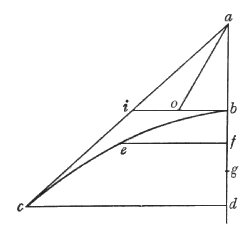
\includegraphics[width=6.25cm,height=5.80cm,keepaspectratio]{images/figura76.png} \end{center}
\end{center}

Sia la semiparabola \emph{bec}, della quale l'ampiezza sia \emph{cd} e l'altezza \emph{db}; quest'ultima, prolungata verso l'alto, incontri in \emph{a} la tangente \emph{ca} alla parabola; e per il vertice \emph{b} sia [condotta] la \emph{bi}, parallela all'orizzonte e alla \emph{cd}. Se, poi, l'ampiezza \emph{cd} è eguale all'intera altezza \emph{da}, \emph{bi} sarà eguale a \emph{ba} e a \emph{bd}; se poniamo che la stessa \emph{ab} sia misura del tempo della caduta per \emph{ab} e del momento di velocità acquistato in \emph{b} in virtù della discesa \emph{ab} a partire dalla quiete in \emph{a}, allora \emph{dc} (che è doppia di \emph{bi}) sarà lo spazio che nel medesimo tempo [il mobile] percorrerà in virtù dell'impeto \emph{ab} deviato sull'orizzontale: ma nel medesimo tempo [il mobile] percorre l'altezza \emph{bd} cadendo lungo \emph{bd} a partire dalla quiete in \emph{b}: dunque, il mobile che, cadendo lungo \emph{ab} a partire dalla quiete in \emph{a}, viene deviato sull'orizzontale con l'impeto \emph{ab}, percorre su di questa uno spazio eguale a \emph{dc}. Ma sopravvenendo il movimento di caduta lungo \emph{bd}, [il mobile] percorre l'altezza \emph{bd} e descrive la parabola \emph{bc}: il suo impeto nell'estremo \emph{c} risulta composto del [l'impeto del moto] trasversale equabile, il cui momento è [rappresentato da] \emph{ab}, e dell'altro momento, acquistato nell'estremo \emph{d}, ossia in \emph{c}, in virtù della discesa \emph{bd}; i quali momenti sono eguali. Se dunque intendiamo che \emph{ab} sia misura di uno dei [due momenti], ad esempio di quello [del moto] trasversale equabile, e che \emph{bi}, eguale a \emph{bd}, sia misura dell'impeto acquistato in \emph{d}, ossia in \emph{c}; l'ipotenusa \emph{ia} sarà la quantità del momento composto di ambedue [i momenti suddetti]: sarà dunque la quantità o misura del momento totale con cui il proietto, che abbia descritto la parabola \emph{bc}, fa impeto in \emph{c}. Tenendo presenti tali considerazioni, si prenda sulla parabola un qualsiasi punto \emph{e}, nel quale si debba determinare l'impeto del proietto. Si conduca l'orizzontale \emph{ef}, e si prenda \emph{bg} media proporzionale tra \emph{bd} e \emph{bf}: poiché abbiamo posto che \emph{ab}, ossia \emph{bd}, sia misura del tempo e del momento di velocità [acquistato] nella caduta \emph{bd} a partire dalla quiete in \emph{b}, sarà \emph{bg} il tempo, ossia la misura del tempo e dell'impeto in \emph{f} del [mobile] proveniente da \emph{b}. Pertanto, se si pone \emph{bo} eguale a \emph{bg}, tracciata la diagonale \emph{ao}, questa sarà la quantità dell'impeto nel punto \emph{e}: infatti si è posta \emph{ab} come determinatrice del tempo e dell'impeto in \emph{b}, il quale [impeto] deviato sull'orizzontale si mantiene sempre lo stesso; \emph{bo} invece determina l'impeto [acquistato] in \emph{f}, ossia in \emph{e}, in virtù della discesa lungo l'altezza \emph{bf} a partire dalla quiete in \emph{b}; ma \emph{ao} è eguale in potenza a questi due \emph{ab} e \emph{bo}. È dunque manifesto quello che si chiedeva.

\speaker{Sagr.} La contemplazione del componimento di questi impeti diversi, e della quantità di quell'impeto che da tal mistione ne risulta, mi giugne tanto nuova, che mi lascia la mente in non piccola confusione: non dico della mistione di due movimenti equabili, benché tra di loro diseguali, fatti uno per la linea orizontale e l'altro per la perpendicolare, ché di questi resto capacissimo farsi un moto in potenza eguale ad amendue i componenti; ma mi nasce confusione nel mescolamento dell'orizontale equabile, e perpendicolare naturalmente accelerato. Però vorrei che insieme digerissimo meglio questa materia.

\speaker{Simp.} Ed io tanto più ne son bisognoso, quanto che non sono ancor totalmente quietato di mente, come bisogna, nelle proposizioni che sono come primi fondamenti dell'altre che gli seguono appresso. Voglio inferire che anco nella mistione de i due moti equabili, orizontale e perpendicolare, vorrei meglio intendere quella potenza del lor composto. Ora, Sig. Salviati, V. S. intende il nostro bisogno e desiderio.

\speaker{Salv.} Il desiderio è molto ragionevole, e tenterò se l'aver io più lungo tempo potuto pensarvi sopra, può agevolare la vostra intelligenza. Ma converrà comportarmi e scusarmi, se nel discorrere andrò replicando buona parte delle cose sin qui poste dall'Autore.

Discorrer determinatamente circa i movimenti e lor velocità o impeti, siano quelli o equabili o naturalmente accelerati, non possiamo noi senza prima determinar della misura che usar vogliamo per misurar tali velocità, come anco della misura del tempo. Quanto alla misura del tempo, già abbiamo la comunemente ricevuta per tutto, delle ore, minuti primi e secondi etc.; e come per misura del tempo ci è la detta comune, ricevuta da tutti, così bisogna assegnarne una per le velocità, che appresso tutti sia comunemente intesa e ricevuta, cioè che appresso tutti sia l'istessa. Atta per tale uso ha stimato l'Autore, come si è dichiarato, esser la velocità de i gravi naturalmente descendenti, de i quali le crescenti velocità in tutte le parti del mondo serbano l'istesso tenore; sì che quel grado di velocità che (per esempio) acquista una palla di piombo d'una libra nell'esser, partendosi dalla quiete, scesa perpendicolarmente quanto è l'altezza di una picca, è sempre e in tutti i luoghi il medesimo, e per ciò accomodatissimo per esplicar la quantità dell'impeto derivante dalla scesa naturale. Resta poi il trovar modo di determinare anco la quantità dell'impeto in un moto equabile in guisa tale, che tutti coloro che circa di quello discorrino, si formino l'istesso concetto della grandezza e velocità sua, sì che uno non se lo figuri più veloce e un altro meno, onde poi nel congiugnere e mescolar questo da sé concepito equabile con lo statuito moto accelerato, da diversi uomini ne vengano formati diversi concetti di diverse grandezze d'impeti. Per determinare e rappresentare cotal impeto e velocità particolare, non ha trovato il nostro Autore altro mezo più accomodato, che 'l servirsi dell'impeto che va acquistando il mobile nel moto naturalmente accelerato del quale qualsivoglia momento acquistato, convertito in moto equabile, ritien la sua velocità limitata precisamente, e tanta, che in altrettanto tempo quanto fu quello della scesa passa doppio spazio dell'altezza dalla quale è caduto. Ma perché questo è punto principale nella materia che si tratta, è bene con qualche esempio particolare farsi perfettamente intendere.

Ripigliando dunque la velocità e l'impeto acquistato dal grave cadente, come dicemmo, dall'altezza d'una picca, della quale velocità vogliamo servirci per misura di altre velocità ed impeti in altre occasioni; e posto, per esempio, che il tempo di tal caduta sia 4 minuti secondi d'ora; per ritrovar da questa tal misura quanto fusse l'impeto del cadente da qualsivoglia altra altezza maggiore o minore, non doviamo dalla proporzione la quale quest'altra altezza avesse con l'altezza d'una picca, argomentare e concludere la quantità dell'impeto acquistato in questa seconda altezza, stimando, per esempio, che il cadente da quadrupla altezza avesse acquistato quadrupla velocità, perché ciò è falso: imperò che non cresce o cala la velocità nel moto naturalmente accelerato secondo la proporzione degli spazii, ma ben secondo quella de i tempi, della quale quella degli spazii è maggiore in duplicata proporzione, come già fu dimostrato. Però, quando noi avessimo in una linea retta assegnatane una parte per misura della velocità, ed anco del tempo e dello spazio in tal tempo passato (ché per brevità tutte tre queste grandezze con un'istessa linea spesse volte vengono rappresentate), per trovar la quantità del tempo e 'l grado di velocità che il mobile medesimo in altra distanza arebbe acquistato, ciò otterremo noi non immediatamente da questa seconda distanza, ma dalla linea che tra le due distanze sarà media proporzionale. Ma con un esempio meglio mi dichiaro.


\begin{center}
~ \begin{center} 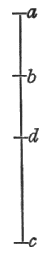
\includegraphics[width=1.25cm,height=6.48cm,keepaspectratio]{images/figura77.png} \end{center}
\end{center}

Nella linea \emph{ac}, perpendicolare all'orizonte, intendasi la parte \emph{ab} essere uno spazio passato da un grave naturalmente descendente di moto accelerato; il tempo del qual passaggio, potendo io rappresentarlo con qualsivoglia linea, voglio per brevità figurarlo esser quanto la medesima linea \emph{ab}; e parimente per misura dell'impeto e velocità acquistata per tal moto pongo pur l'istessa linea \emph{ab}: sì che di tutti gli spazii che nel progresso del discorso si hanno a considerare, la misura sia la parte \emph{ab}. Stabilite ad arbitrio nostro sotto una sola grandezza \emph{ab} queste 3 misure di generi di quantità diversissimi, cioè di spazii, di tempi e di impeti, siaci proposto di dover determinare, nell'assegnato spazio e altezza \emph{ac}, quanto sia per essere il tempo della scesa del cadente da l'\emph{a} in \emph{c}, e quanto l'impeto che in esso termine \emph{c} si troverà avere acquistato, in relazione al tempo ed all'impeto misurati per la \emph{ab}. L'uno e l'altro quesito si determinerà pigliando delle due linee \emph{ac}, \emph{ab} la media proporzionale \emph{ad}; affermando, il tempo della caduta per tutto lo spazio \emph{ac} esser quanto il tempo \emph{ad} in relazione al tempo \emph{ab}, posto da principio per la quantità del tempo nella scesa \emph{ab}. Diremo parimente, l'impeto o grado di velocità che otterrà 'l cadente nel termine \emph{c}, in relazione all'impeto che ebbe in \emph{b}, esser quale è la medesima linea \emph{ad} in relazione alla \emph{ab}, essendo che la velocità cresce con la medesima proporzione che cresce il tempo: la qual conclusione se ben fu presa come postulato, pur tuttavia volse l'Autore esplicarne l'applicazione di sopra, alla Proposizion terza.

Ben compreso e stabilito questo punto, venghiamo alla considerazione dell'impeto derivante da 2 moti composti; uno de i quali sia composto dell'orizontale e sempre equabile, e del perpendicolare all'orizonte e esso ancora equabile; ma l'altro sia composto dell'orizontale, pur sempre equabile, e del perpendicolare naturalmente accelerato. Se amendue saranno equabili, già s'è visto come l'impeto resultante dalla composizione di amendue è in potenza equale ad amendue, come per chiara intelligenza esemplificheremo così.


\begin{center}
\begin{center} 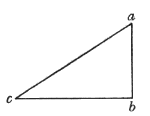
\includegraphics[width=3.75cm,height=2.90cm,keepaspectratio]{images/figura78.png} \end{center}
\end{center}

Intendasi, il mobile descendente per la perpendicolare \emph{ab} aver, per esempio, 3 gradi d'impeto equabile, ma, trasportato per la \emph{ab} verso \emph{c}, esser tal velocità ed impeto di 4 gradi, sì che nel tempo medesimo che scendendo passerebbe nella perpendicolare, v. g., 3 braccia, nella orizontale ne passerebbe 4: ma nel composto di amendue le velocità viene, nel medesimo tempo, dal punto \emph{a} nel termine \emph{c}, caminando sempre per la diagonale \emph{ac}, la quale non è lunga 7, quanto sarebbe la composta delle 2, \emph{ab} 3 e \emph{bc} 4, ma è 5; la qual 5 è in potenza equale alle due 3 e 4. Imperò che, fatti li quadrati del 3 e del 4, che sono 9 e 16, e questi congiunti insieme, fanno 25 per il quadrato di \emph{ac}, il quale alli due quadrati di \emph{ab} e di \emph{bc} è eguale; onde la \emph{ac} sarà quanto è il lato, o vogliam dir la radice, del quadrato 25, che è 5. Per regola dunque ferma e sicura, quando si debba assegnare la quantità dell'impeto resultante da 2 impeti dati, uno orizontale e l'altro perpendicolare ed amendue equabili, si deve di amendue fare i quadrati, e, componendogli insieme, estrar la radice del composto, la quale ci darà la quantità dell'impeto composto di amendue quelli. E così nell'esempio posto, quel mobile che in virtù del moto perpendicolare arebbe percosso sopra l'orizonte con 3 gradi di forza, e col moto solo orizontale arebbe percosso in \emph{c} con gradi 4, percotendo con amendue gl'impeti congiunti, il colpo sarà come quello del percuziente mosso con gradi 5 di velocità e di forza; e questa tal percossa sarebbe del medesimo valore in tutti i punti della diagonale \emph{ac}, per esser sempre gl'impeti composti i medesimi, non mai cresciuti o diminuiti.

Veggiamo ora quello che accaschi nel comporre il moto orizontale equabile con un moto perpendicolare all'orizonte, il quale, cominciando dalla quiete, vadia naturalmente accelerandosi. Già è manifesto che la diagonale, che è la linea del moto composto di questi due, non è una linea retta, ma semiparabolica, come si è dimostrato; nella quale l'impeto va sempre crescendo, mercé del continuo crescimento della velocità del moto perpendicolare. Là onde, per determinar qual sia l'impeto in un assegnato punto di essa diagonale parabolica, prima bisogna assegnar la quantità dell'impeto uniforme orizontale, e poi investigar qual sia l'impeto del cadente nell'assegnato punto, il che non si può determinare senza la considerazione del tempo decorso dal principio della composizione de i 2 moti, la qual considerazione di tempo non si richiede nella composizione de i moti equabili, le velocità ed impeti de i quali son sempre i medesimi; ma qui, dove entra nella mistione un moto che, cominciando dalla somma tardità, va crescendo la velocità conforme alla continuazion del tempo, è necessario che la quantità del tempo ci manifesti la quantità del grado di velocità nell'assegnato punto: ché quanto al resto poi, l'impeto composto di questi 2 è (come nei moti uniformi) eguale in potenza ad amendue i componenti. Ma qui ancora meglio mi dichiaro con un esempio.


\begin{center}
\begin{center} 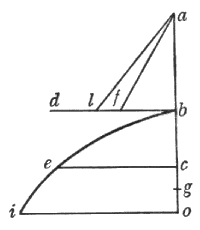
\includegraphics[width=5.00cm,height=5.75cm,keepaspectratio]{images/figura79.png} \end{center}
\end{center}

Sia nella perpendicolare all'orizonte \emph{ac} presa qualsivoglia parte \emph{ab}, la quale figuro che serva per misura dello spazio del moto naturale fatto in essa perpendicolare, e parimente sia misura del tempo ed anco del grado di velocità, o vogliam dire de gl'impeti: è primieramente manifesto, che se l'impeto del cadente in \emph{b} dalla quiete in \emph{a} si convertirà sopra la \emph{bd}, parallela all'orizonte, in moto equabile, la quantità della sua velocità sarà tanta, che nel tempo \emph{ab} passerà uno spazio doppio dello spazio \emph{ab}; e tanta sia la linea \emph{bd}. Posta poi la \emph{bc} eguale alla \emph{ba}, e tirata la parallela \emph{ce} alla \emph{bd}, e ad essa eguale, descriveremo per i punti \emph{b}, \emph{e} la linea parabolica \emph{bei}. E perché nel tempo \emph{ab} con l'impeto \emph{ab} si passa l'orizontale \emph{bd} o \emph{ce}, doppia della \emph{ab}, e passasi ancora in altrettanto tempo la perpendicolare \emph{bc} con acquisto d'impeto in \emph{c} eguale al medesimo orizontale; adunque il mobile, in tanto tempo quanto è \emph{ab}, si troverà dal \emph{b} giunto in \emph{e} per la parabola \emph{be} con un impeto composto di due, ciascheduno eguale all'impeto \emph{ab}: e perché l'uno di essi è orizontale e l'altro perpendicolare, l'impeto composto di essi sarà in potenza eguale ad amendue, cioè doppio di uno; onde, posta la \emph{bf} eguale alla \emph{ba} e tirata la diagonale \emph{af}, l'impeto e la percossa in \emph{e} sarà maggiore della percossa in \emph{b} del cadente dall'altezza \emph{a}, o vero della percossa dell'impeto orizontale per la \emph{bd}, secondo la proporzione di \emph{af} ad \emph{ab}. Ma quando, ritenendo pur sempre la \emph{ba} per misura dello spazio della caduta dalla quiete in \emph{a} sino in \emph{b} e per misura del tempo e dell'impeto del cadente acquistato in \emph{b}, l'altezza \emph{bo} non fusse eguale, ma maggiore della \emph{ab}, presa la \emph{bg} media proporzionale tra esse \emph{ab}, \emph{bo}, sarebbe essa \emph{bg} misura del tempo e dell'impeto in \emph{o}, per la caduta nell'altezza \emph{bo} acquistato in \emph{o}; e lo spazio per l'orizontale, il quale passato con l'impeto \emph{ab} nel tempo \emph{ab} sarebbe doppio della \emph{ab}, sarà in tutta la durazion del tempo \emph{bg} tanto maggiore, quanto a proporzione la \emph{bg} è maggiore della \emph{ba}. Posta dunque la \emph{lb} eguale alla \emph{bg}, e tirata la diagonale \emph{al}, avremo da essa la quantità composta delli 2 impeti orizontale e perpendicolare, da i quali si descrive la parabola; de i quali l'orizontale ed equabile è l'acquistato in \emph{b} per la caduta \emph{ab}, e l'altro è l'acquistato in \emph{o}, o vogliam dire in \emph{i}, per la caduta \emph{bo}, il cui tempo fu \emph{bg}, come anco la quantità del suo momento. E con simil discorso investigheremo l'impeto nel termine estremo della parabola, quando l'altezza sua fusse minore della sublimità \emph{ab}, prendendo tra amendue la media; la quale posta nell'orizontale in luogo della \emph{bf}, e congiunta la diagonale, come \emph{af}, aremo da questa la quantità dell'impeto nell'estremo termine della parabola.

A quanto sin qui è considerato circa questi impeti, colpi o vogliam dir percosse, di tali proietti, convien aggiugnere un'altra molto necessaria considerazione: e questa è, che non basta por mente alla sola velocità del proietto per ben determinare della forza ed energia della percossa, ma convien chiamare a parte ancora lo stato e condizione di quello che riceve la percossa, nell'efficacia della quale esso per più rispetti ha gran participazione e interesse. E prima, non è chi non intenda che la cosa percossa intanto patisce violenza dalla velocità del percuziente, in quanto ella se gli oppone, e frena in tutto o in parte il moto di quello: ché se il colpo arriverà sopra tale che ceda alla velocità del percuziente senza resistenza alcuna, tal colpo sarà nullo; e colui che corre per ferir con lancia il suo nimico, se nel sopraggiugnerlo accaderà che quello si muova fuggendo con pari velocità, non farà colpo, e l'azzione sarà un semplice toccare senza offendere. Ma se la percossa verrà ricevuta in un oggetto che non in tutto ceda al percuziente, ma solamente in parte, la percossa danneggerà, ma non con tutto l'impeto, ma solo con l'eccesso della velocità di esso percuziente sopra la velocità della ritirata e cedenza del percosso: sì che, se, v. g., il percuziente arriverà con 10 gradi di velocità sopra 'l percosso, il quale, cedendo in parte, si ritiri con gradi 4, l'impeto e percossa sarà come di gradi 6. E finalmente, intera e massima sarà la percossa, per la parte del percuziente, quando il percosso nulla ceda, ma interamente si opponga, e fermi tutto 'l moto del percuziente; se però questo può accadere. Ed ho detto \emph{per la parte del percuziente}, perché quando il percosso si movesse con moto contrario verso 'l percuziente, il colpo e l'incontro si farebbe tanto più gagliardo, quanto le 2 velocità contrarie unite son maggiori che la sola del percuziente. Di più, conviene anco avvertire che il ceder più o meno può derivare non solamente dalla qualità della materia più o meno dura, come se sia di ferro, di piombo o di lana etc., ma dalla positura del corpo che riceve la percossa: la qual positura se sarà tale che 'l moto del percuziente la vadia a investire ad angoli retti, l'impeto del colpo sarà il massimo; ma se 'l moto verrà obbliquamente e, come diciamo noi, a scancìo, il colpo sarà più debole, e più e più secondo la maggiore obbliquità; perché in oggetto in tal modo situato, ancor che di materia sodissima, non si spegne e ferma tutto l'impeto e moto del percuziente, il quale, sfuggendo, passa oltre, continuando almeno in qualche parte a muoversi sopra la superficie del resistente opposto. Quando dunque si è di sopra determinato della grandezza dell'impeto del proietto nell'estremità della linea parabolica, si deve intendere della percossa ricevuta sopra una linea ad angoli retti ad essa parabolica o vero alla tangente la parabola nel detto punto; perché, se ben quel moto è composto d'un orizontale e d'un perpendicolare, l'impeto né sopra l'orizontale né sopra 'l piano eretto all'orizonte è il massimo, venendo sopra amendue ricevuto obbliquamente.

\speaker{Sagr.} Il ricordar V. S. questi colpi e queste percosse mi ha risvegliato nella mente un problema o vogliam dire questione mecanica, della quale non ho trovato appresso autore alcuno la soluzione, né cosa che mi scemi la maraviglia o al meno in parte mi quieti l'intelletto. E 'l dubbio e lo stupor mio consiste nel non restar capace onde possa derivare, e da qual principio possa dependere, l'energia e la forza immensa che si vede consistere nella percossa, mentre col semplice colpo d'un martello, che non abbia peso maggiore di 8 o 10 libre, veggiamo superarsi resistenze tali, le quali non cederanno al peso d'un grave che, senza percossa, vi faccia impeto, solamente calcando e premendo, benché la gravità di quello passi molte centinaia di libre. Io vorrei pur trovar modo di misurar la forza di questa percossa; la quale non penso però che sia infinita, anzi stimo che ella abbia il suo termine da potersi pareggiare e finalmente regolare con altre forze di gravità prementi, o di leve o di viti o di altri strumenti mecanici, de i quali io a sodisfazione resto capace della multiplicazione della forza loro.

\speaker{Salv.} V. S. non è solo, nella maraviglia dell'effetto e nella oscurità della cagione di così stupendo accidente. Io vi pensai per alcun tempo in vano, accrescendo sempre la confusione, sin che finalmente, incontrandomi nel nostro Academico, da esso ricevei doppia consolazione: prima, nel sentire come egli ancora era stato lungo tempo nelle medesime tenebre; e poi nel dirmi che, dopo l'avervi in vita sua consumate molte migliara di ore specolando e filosofando, ne aveva conseguite alcune cognizioni lontane dai nostri primi concetti, e però nuove e per la novità ammirande. E perché ormai so che la curiosità di V. S. volentieri sentirebbe quei pensieri che si allontanano dall'opinabile, non aspetterò la sua richiesta, ma gli do parola che, spedita che avremo la lettura di questo trattato de i proietti, gli spiegherò tutte quelle fantasie, o vogliàn dire stravaganze, che de i discorsi dell'Accademico mi son rimaste nella memoria. In tanto seguitiamo le proposizioni dell'Autore.

\textbf{PROPOSIZIONE 5. PROBLEMA}\\ Sul prolungamento dell'asse di una parabola data determinare in alto un punto, cadendo dal quale [un mobile] descriva quella parabola stessa.

\textbf{COROLLARIO}\\ Di qui risulta che la metà della base, ossia la metà dell'ampiezza di una semiparabola (che è poi la quarta parte dell'ampiezza della intera parabola) è media proporzionale tra la sua altezza e quella sublimità, cadendo dalla quale il mobile descrive la semiparabola stessa.

\textbf{PROPOSIZIONE 6. PROBLEMA}\\ Date la sublimità e l'altezza di una semiparabola, trovare l'ampiezza.


\begin{center}
\begin{center} 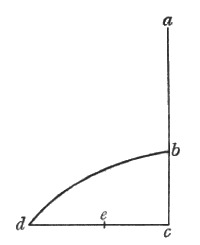
\includegraphics[width=5.00cm,height=6.12cm,keepaspectratio]{images/figura80.png} \end{center}
\end{center}

Sia la perpendicolare \emph{ac} alla linea orizzontale \emph{dc}, e su di essa siano date l'altezza \emph{cb} e la sublimità \emph{ba}: bisogna trovare sull'orizzontale \emph{cd} l'ampiezza della semiparabola descritta [a partire] dalla sublimità \emph{ba} e con altezza \emph{bc}. Si prenda la media proporzionale tra \emph{cb} e \emph{ba} e si ponga \emph{cd} doppia di essa: dico che \emph{cd} è l'ampiezza cercata. E ciò appare manifesto dal precedente [corollario].

\textbf{TEOREMA. PROPOSIZIONE 7}\\ Fra i proietti che descrivono semiparabole di eguale ampiezza, si richiede minor impeto in quello che descrive quella [parabola] la cui ampiezza è doppia della propria altezza, che non in qualsiasi altro proietto.

\textbf{COROLLARIO}\\ Da ciò è manifesto che, per converso, in un proietto lanciato dall'estremo \emph{d} si richiede minor impeto per [descrivere] la semiparabola \emph{db} che per [descrivere] qualsiasi altra semiparabola con elevazione maggiore o minore dell'elevazione della semiparabola \emph{db}, [elevazione fatta] secondo la tangente \emph{ad}, che forma sopra l'orizzonte un angolo semiretto. Stando così le cose, risulta che, se dall'estremo \emph{d} vengono lanciati proietti con un medesimo impeto, ma secondo differenti elevazioni, la proiezione massima, ossia la semiparabola o parabola intera di massima ampiezza, sarà quella che verrà fatta con l'elevazione di mezzo angolo retto; invece tutte le altre, fatte ad angoli maggiori o minori, saranno minori.

\speaker{Sagr.} Piena di maraviglia e di diletto insieme è la forza delle dimostrazioni necessarie, quali sono le sole matematiche. Gia sapevo io, per fede prestata alle relazioni di più bombardieri, che di tutti i tiri di volata dell'artiglieria, o del mortaro, il massimo, cioè quello che in maggior lontananza caccia la palla, era il fatto all'elevazione di mezo angolo retto, che essi dicono del sesto punto della squadra; ma l'intender la cagione onde ciò avvenga, supera d'infinito intervallo la semplice notizia auta dalle altrui attestazioni, ed anco da molte replicate esperienze.

\speaker{Salv.} V. S. molto veridicamente discorre: e la cognizione d'un solo effetto acquistata per le sue cause ci apre l'intelletto a 'ntendere ed assicurarci d'altri effetti senza bisogno di ricorrere alle esperienze, come appunto avviene nel presente caso; dove, guadagnata per il discorso dimostrativo la certezza dell'essere il massimo di tutti i tiri di volata quello dell'elevazione dell'angolo semiretto, ci dimostra l'Autore quello che forse per l'esperienza non è stato osservato: e questo è, che de gli altri tiri, quelli sono tra di loro eguali, le elevazioni de i quali superano o mancano per angoli eguali dalla semiretta: sì che le palle tirate dall'orizonte, una secondo l'elevazione di 7 punti e l'altra di 5, andranno a ferir su l'orizonte in lontananze eguali, e così eguali saranno i tiri di 8 e di 4 punti, di 9 e di 3, etc. Or sentiamone la dimostrazione.

\textbf{TEOREMA. PROPOSIZIONE 8}\\ Le ampiezze delle parabole descritte da proietti, lanciati con un medesimo impeto e secondo elevazioni che superano o mancano per angoli eguali dall'angolo semiretto, sono tra di loro eguali.

\textbf{TEOREMA. PROPOSIZIONE 9}\\ Eguali sono le ampiezze di quelle parabole, le cui altezze e sublimità sono tra di loro inversamente proporzionali.

\textbf{TEOREMA. PROPOSIZIONE 10}\\ L'impeto o momento di una qualsiasi semiparabola è eguale al momento di un mobile, che cada naturalmente secondo una perpendicolare all'orizzonte, la quale sia lunga quanto la linea composta dalla sublimità e dall'altezza della semiparabola.

\textbf{COROLLARIO}\\ Da ciò risulta che sono tra loro eguali gli impeti di tutte le semiparabole, in ciascuna delle quali la somma dell'altezza con la [rispettiva] sublimità è sempre la medesima.

\textbf{PROBLEMA. PROPOSIZIONE 11}\\ Dati l'impeto e l'ampiezza di una semiparabola, trovare l'altezza.

\textbf{PROBLEMA. PROPOSIZIONE 12}\\ Calcolare e ordinare in una tavola le ampiezze di tutte le semiparabole descritte da proietti lanciati col medesimo impeto.

\speaker{Sagr.} Mi manca, per l'intera intelligenza di questa dimostrazione, il saper come sia vero che la terza proporzionale delle \emph{bf}, \emph{bi} sia (come dice l'Autore) necessariamente maggiore della \emph{fa}.

\speaker{Salv.} Tal conseguenza mi par che si possa dedurre in tal modo. Il quadrato della media di tre linee proporzionali è eguale al rettangolo dell'altre due; onde il quadrato della \emph{bi}, o della \emph{bd} ad essa eguale, deve esser eguale al rettangolo della prima \emph{fb} nella terza da ritrovarsi: la qual terza è necessario che sia maggiore della \emph{fa}, perché il rettangolo della \emph{bf} in \emph{fa} è minore del quadrato \emph{bd}, ed il mancamento è quanto il quadrato della \emph{df}, come dimostra Euclide in una del secondo. Devesi anco avvertire che il punto \emph{f}, che divide la tangente \emph{eb} in mezo, altre molte volte cadrà sopra 'l punto \emph{a}, ed una volta anco nell'istesso \emph{a}; ne i quali casi è per sé noto che la terza proporzionale della metà della tangente e della \emph{bi} (che dà la subblimità) è tutta sopra la \emph{a}. Ma l'Autore ha preso il caso dove non era manifesto che la detta terza proporzionale fusse sempre maggiore della \emph{fa}, e che però, aggiunta sopra 'l punto \emph{f}, passasse oltre alla parallela \emph{ag}. Or seguitiamo.


\begin{center}
\textbf{Ampiezze delle semiparabole il cui impeto sia il medesimo.}
\end{center}

\begin{center}
\small
\begin{tabular}{r r r @{\hspace{2em}} r r r}
\toprule
\multicolumn{6}{c}{\textbf{\textsc{Gradi di Elevazione}}} \\
\midrule
\textbf{\textit{Gr.}} & \textit{Amp.} & \textbf{\textit{Gr.}} & \textbf{\textit{Gr.}} & \textit{Amp.} & \textbf{\textit{Gr.}} \\
\midrule
\textcolor{rubric}{\textit{45}} & \textit{10000} &  & \textcolor{rubric}{\textit{69}} & \textit{6692} & \textit{21} \\
\textcolor{rubric}{\textit{46}} & \textit{9994} & \textcolor{rubric}{\textit{44}} & \textcolor{rubric}{\textit{70}} & \textit{6428} & \textit{20} \\
\textcolor{rubric}{\textit{47}} & \textit{9976} & \textcolor{rubric}{\textit{43}} & \textcolor{rubric}{\textit{71}} & \textit{6157} & \textit{19} \\
\textcolor{rubric}{\textit{48}} & \textit{9945} & \textcolor{rubric}{\textit{42}} & \textcolor{rubric}{\textit{72}} & \textit{5878} & \textit{18} \\
\textcolor{rubric}{\textit{49}} & \textit{9902} & \textcolor{rubric}{\textit{41}} & \textcolor{rubric}{\textit{73}} & \textit{5592} & \textit{17} \\
\textcolor{rubric}{\textit{50}} & \textit{9848} & \textcolor{rubric}{\textit{40}} & \textcolor{rubric}{\textit{74}} & \textit{5300} & \textit{16} \\
\textcolor{rubric}{\textit{51}} & \textit{9782} & \textcolor{rubric}{\textit{39}} & \textcolor{rubric}{\textit{75}} & \textit{5000} & \textit{15} \\
\textcolor{rubric}{\textit{52}} & \textit{9704} & \textcolor{rubric}{\textit{38}} & \textcolor{rubric}{\textit{76}} & \textit{4694} & \textit{14} \\
\textcolor{rubric}{\textit{53}} & \textit{9612} & \textcolor{rubric}{\textit{37}} & \textcolor{rubric}{\textit{77}} & \textit{4383} & \textit{13} \\
\textcolor{rubric}{\textit{54}} & \textit{9511} & \textcolor{rubric}{\textit{36}} & \textcolor{rubric}{\textit{78}} & \textit{4067} & \textit{12} \\
\textcolor{rubric}{\textit{55}} & \textit{9396} & \textcolor{rubric}{\textit{35}} & \textcolor{rubric}{\textit{79}} & \textit{3746} & \textit{11} \\
\textcolor{rubric}{\textit{56}} & \textit{9272} & \textcolor{rubric}{\textit{34}} & \textcolor{rubric}{\textit{80}} & \textit{3420} & \textit{10} \\
\textcolor{rubric}{\textit{57}} & \textit{9136} & \textcolor{rubric}{\textit{33}} & \textcolor{rubric}{\textit{81}} & \textit{3090} & \textit{9} \\
\textcolor{rubric}{\textit{58}} & \textit{8989} & \textcolor{rubric}{\textit{32}} & \textcolor{rubric}{\textit{82}} & \textit{2756} & \textit{8} \\
\textcolor{rubric}{\textit{59}} & \textit{8829} & \textcolor{rubric}{\textit{31}} & \textcolor{rubric}{\textit{83}} & \textit{2419} & \textit{7} \\
\textcolor{rubric}{\textit{60}} & \textit{8659} & \textcolor{rubric}{\textit{30}} & \textcolor{rubric}{\textit{84}} & \textit{2079} & \textit{6} \\
\textcolor{rubric}{\textit{61}} & \textit{8481} & \textcolor{rubric}{\textit{29}} & \textcolor{rubric}{\textit{85}} & \textit{1736} & \textit{5} \\
\textcolor{rubric}{\textit{62}} & \textit{8290} & \textcolor{rubric}{\textit{28}} & \textcolor{rubric}{\textit{86}} & \textit{1391} & \textit{4} \\
\textcolor{rubric}{\textit{63}} & \textit{8090} & \textcolor{rubric}{\textit{27}} & \textcolor{rubric}{\textit{87}} & \textit{1044} & \textit{3} \\
\textcolor{rubric}{\textit{64}} & \textit{7880} & \textcolor{rubric}{\textit{26}} & \textcolor{rubric}{\textit{88}} & \textit{698} & \textit{2} \\
\textcolor{rubric}{\textit{65}} & \textit{7660} & \textcolor{rubric}{\textit{25}} & \textcolor{rubric}{\textit{89}} & \textit{349} & \textit{1} \\
\textcolor{rubric}{\textit{66}} & \textit{7431} & \textcolor{rubric}{\textit{24}} &  &  &  \\
\textcolor{rubric}{\textit{67}} & \textit{7191} & \textcolor{rubric}{\textit{23}} &  &  &  \\
\textcolor{rubric}{\textit{68}} & \textit{6944} & \textcolor{rubric}{\textit{22}} &  &  &  \\
\bottomrule
\end{tabular}
\end{center}

Non sarà inutile, mercé l'ausilio della precedente tavola, comporne un'altra che unisca le altezze delle medesime semiparabole descritte da proietti lanciati con lo stesso impeto.


\begin{center}
\textbf{Altezze delle semiparabole il cui impeto sia il medesimo.}
\end{center}

\begin{center}
\small
\begin{tabular}{r r @{\hspace{1.5em}} r r @{\hspace{1.5em}} r r @{\hspace{1.5em}} r r}
\toprule
\multicolumn{8}{c}{\textbf{\textsc{Gradi di Elevazione}}} \\
\midrule
\textbf{\textit{Gr.}} & \textit{Alt.} & \textbf{\textit{Gr.}} & \textit{Alt.} & \textbf{\textit{Gr.}} & \textit{Alt.} & \textbf{\textit{Gr.}} & \textit{Alt.} \\
\midrule
\textcolor{rubric}{\textit{1}} & \textit{3} & \textcolor{rubric}{\textit{46}} & \textit{5173} & \textcolor{rubric}{\textit{25}} & \textit{1786} & \textcolor{rubric}{\textit{70}} & \textit{8830} \\
\textcolor{rubric}{\textit{2}} & \textit{13} & \textcolor{rubric}{\textit{47}} & \textit{5346} & \textcolor{rubric}{\textit{26}} & \textit{1922} & \textcolor{rubric}{\textit{71}} & \textit{8940} \\
\textcolor{rubric}{\textit{3}} & \textit{28} & \textcolor{rubric}{\textit{48}} & \textit{5523} & \textcolor{rubric}{\textit{27}} & \textit{2061} & \textcolor{rubric}{\textit{72}} & \textit{9045} \\
\textcolor{rubric}{\textit{4}} & \textit{50} & \textcolor{rubric}{\textit{49}} & \textit{5698} & \textcolor{rubric}{\textit{28}} & \textit{2204} & \textcolor{rubric}{\textit{73}} & \textit{9144} \\
\textcolor{rubric}{\textit{5}} & \textit{76} & \textcolor{rubric}{\textit{50}} & \textit{5868} & \textcolor{rubric}{\textit{29}} & \textit{2351} & \textcolor{rubric}{\textit{74}} & \textit{9240} \\
\textcolor{rubric}{\textit{6}} & \textit{108} & \textcolor{rubric}{\textit{51}} & \textit{6038} & \textcolor{rubric}{\textit{30}} & \textit{2499} & \textcolor{rubric}{\textit{75}} & \textit{9330} \\
\textcolor{rubric}{\textit{7}} & \textit{150} & \textcolor{rubric}{\textit{52}} & \textit{6207} & \textcolor{rubric}{\textit{31}} & \textit{2653} & \textcolor{rubric}{\textit{76}} & \textit{9415} \\
\textcolor{rubric}{\textit{8}} & \textit{194} & \textcolor{rubric}{\textit{53}} & \textit{6379} & \textcolor{rubric}{\textit{32}} & \textit{2810} & \textcolor{rubric}{\textit{77}} & \textit{9493} \\
\textcolor{rubric}{\textit{9}} & \textit{245} & \textcolor{rubric}{\textit{54}} & \textit{6546} & \textcolor{rubric}{\textit{33}} & \textit{2967} & \textcolor{rubric}{\textit{78}} & \textit{9567} \\
\textcolor{rubric}{\textit{10}} & \textit{302} & \textcolor{rubric}{\textit{55}} & \textit{6710} & \textcolor{rubric}{\textit{34}} & \textit{3128} & \textcolor{rubric}{\textit{79}} & \textit{9636} \\
\textcolor{rubric}{\textit{11}} & \textit{365} & \textcolor{rubric}{\textit{56}} & \textit{6873} & \textcolor{rubric}{\textit{35}} & \textit{3289} & \textcolor{rubric}{\textit{80}} & \textit{9698} \\
\textcolor{rubric}{\textit{12}} & \textit{432} & \textcolor{rubric}{\textit{57}} & \textit{7033} & \textcolor{rubric}{\textit{36}} & \textit{3456} & \textcolor{rubric}{\textit{81}} & \textit{9755} \\
\textcolor{rubric}{\textit{13}} & \textit{506} & \textcolor{rubric}{\textit{58}} & \textit{7190} & \textcolor{rubric}{\textit{37}} & \textit{3621} & \textcolor{rubric}{\textit{82}} & \textit{9806} \\
\textcolor{rubric}{\textit{14}} & \textit{585} & \textcolor{rubric}{\textit{59}} & \textit{7348} & \textcolor{rubric}{\textit{38}} & \textit{3793} & \textcolor{rubric}{\textit{83}} & \textit{9851} \\
\textcolor{rubric}{\textit{15}} & \textit{670} & \textcolor{rubric}{\textit{60}} & \textit{7502} & \textcolor{rubric}{\textit{39}} & \textit{3962} & \textcolor{rubric}{\textit{84}} & \textit{9890} \\
\textcolor{rubric}{\textit{16}} & \textit{760} & \textcolor{rubric}{\textit{61}} & \textit{7649} & \textcolor{rubric}{\textit{40}} & \textit{4132} & \textcolor{rubric}{\textit{85}} & \textit{9924} \\
\textcolor{rubric}{\textit{17}} & \textit{855} & \textcolor{rubric}{\textit{62}} & \textit{7796} & \textcolor{rubric}{\textit{41}} & \textit{4302} & \textcolor{rubric}{\textit{86}} & \textit{9951} \\
\textcolor{rubric}{\textit{18}} & \textit{955} & \textcolor{rubric}{\textit{63}} & \textit{7939} & \textcolor{rubric}{\textit{42}} & \textit{4477} & \textcolor{rubric}{\textit{87}} & \textit{9972} \\
\textcolor{rubric}{\textit{19}} & \textit{1060} & \textcolor{rubric}{\textit{64}} & \textit{8078} & \textcolor{rubric}{\textit{43}} & \textit{4654} & \textcolor{rubric}{\textit{88}} & \textit{9987} \\
\textcolor{rubric}{\textit{20}} & \textit{1170} & \textcolor{rubric}{\textit{65}} & \textit{8214} & \textcolor{rubric}{\textit{44}} & \textit{4827} & \textcolor{rubric}{\textit{89}} & \textit{9998} \\
\textcolor{rubric}{\textit{21}} & \textit{1285} & \textcolor{rubric}{\textit{66}} & \textit{8346} & \textcolor{rubric}{\textit{45}} & \textit{5000} & \textcolor{rubric}{\textit{90}} & \textit{10000} \\
\textcolor{rubric}{\textit{22}} & \textit{1402} & \textcolor{rubric}{\textit{67}} & \textit{8474} &  &  &  &  \\
\textcolor{rubric}{\textit{23}} & \textit{1527} & \textcolor{rubric}{\textit{68}} & \textit{8597} &  &  &  &  \\
\textcolor{rubric}{\textit{24}} & \textit{1685} & \textcolor{rubric}{\textit{69}} & \textit{8715} &  &  &  &  \\
\bottomrule
\end{tabular}
\end{center}

\speaker{Sagr.} Questa vedrò io molto volentieri, mentre che per essa potrò venir in cognizione della differenza de gl'impeti e delle forze che si ricercano per cacciar il proietto nella medesima lontananza con tiri che chiamano di volata; la qual differenza credo che sia grandissima secondo le diverse elevazioni: sì che, per esempio, se altri volesse alla elevazione di 3 o 4 gradi, o di 87 o 88, far cader la palla dove fu cacciata alla elevazione di 45 (dove si è mostrato ricercarsi l'impeto minimo), credo si ricercherebbe un eccesso immenso di forza.

\speaker{Salv.} V. S. stima benissimo; e vedrà che per eseguire l'opera intera in tutte l'elevazioni, bisogna andar a gran passo verso l'impeto infinito. Or veggiamo la costruzzione della tavola.

\textbf{PROBLEMA. PROPOSIZIONE 13}\\ Date le ampiezze delle semiparabole, ordinate nella tavola precedente, supponendo comune l'impeto con cui ciascuna viene descritta, ricavarne le rispettive altezze.

Non sarà inutile presentare una terza tavola, contenente le altezze e le sublimità delle semiparabole aventi la medesima ampiezza.


\begin{center}
\textbf{Tavola contenente le altezze e le sublimità delle semiparabole aventi le medesime ampiezze, cioè di 10.000 parti, calcolata per ogni singolo grado di elevazione.}
\end{center}

\begin{center}
\footnotesize
\renewcommand{\arraystretch}{0.84}
\begin{tabular}{r r r @{\hspace{2.5em}} r r r}
\toprule
\textbf{\textit{Gr.}} & \textbf{\textit{Altit.}} & \textbf{\textit{Subl.}} & \textbf{\textit{Gr.}} & \textbf{\textit{Altit.}} & \textbf{\textit{Subl.}} \\
\midrule
\textcolor{rubric}{\textit{1}} & \textit{87} & \textit{286533} & \textcolor{rubric}{\textit{46}} & \textit{5177} & \textit{4828} \\
\textcolor{rubric}{\textit{2}} & \textit{175} & \textit{142450} & \textcolor{rubric}{\textit{47}} & \textit{5363} & \textit{4662} \\
\textcolor{rubric}{\textit{3}} & \textit{262} & \textit{95802} & \textcolor{rubric}{\textit{48}} & \textit{5553} & \textit{4502} \\
\textcolor{rubric}{\textit{4}} & \textit{349} & \textit{71531} & \textcolor{rubric}{\textit{49}} & \textit{5752} & \textit{4345} \\
\textcolor{rubric}{\textit{5}} & \textit{437} & \textit{57142} & \textcolor{rubric}{\textit{50}} & \textit{5959} & \textit{4196} \\
\textcolor{rubric}{\textit{6}} & \textit{525} & \textit{47573} & \textcolor{rubric}{\textit{51}} & \textit{6174} & \textit{4048} \\
\textcolor{rubric}{\textit{7}} & \textit{614} & \textit{40716} & \textcolor{rubric}{\textit{52}} & \textit{6399} & \textit{3906} \\
\textcolor{rubric}{\textit{8}} & \textit{702} & \textit{35587} & \textcolor{rubric}{\textit{53}} & \textit{6635} & \textit{3765} \\
\textcolor{rubric}{\textit{9}} & \textit{792} & \textit{31565} & \textcolor{rubric}{\textit{54}} & \textit{6882} & \textit{3632} \\
\textcolor{rubric}{\textit{10}} & \textit{881} & \textit{28367} & \textcolor{rubric}{\textit{55}} & \textit{7141} & \textit{3500} \\
\textcolor{rubric}{\textit{11}} & \textit{972} & \textit{25720} & \textcolor{rubric}{\textit{56}} & \textit{7413} & \textit{3372} \\
\textcolor{rubric}{\textit{12}} & \textit{1063} & \textit{23518} & \textcolor{rubric}{\textit{57}} & \textit{7699} & \textit{3247} \\
\textcolor{rubric}{\textit{13}} & \textit{1154} & \textit{21701} & \textcolor{rubric}{\textit{58}} & \textit{8002} & \textit{3123} \\
\textcolor{rubric}{\textit{14}} & \textit{1246} & \textit{20056} & \textcolor{rubric}{\textit{59}} & \textit{8332} & \textit{3004} \\
\textcolor{rubric}{\textit{15}} & \textit{1339} & \textit{18663} & \textcolor{rubric}{\textit{60}} & \textit{8600} & \textit{2887} \\
\textcolor{rubric}{\textit{16}} & \textit{1434} & \textit{17405} & \textcolor{rubric}{\textit{61}} & \textit{9020} & \textit{2771} \\
\textcolor{rubric}{\textit{17}} & \textit{1529} & \textit{16355} & \textcolor{rubric}{\textit{62}} & \textit{9403} & \textit{2658} \\
\textcolor{rubric}{\textit{18}} & \textit{1624} & \textit{15389} & \textcolor{rubric}{\textit{63}} & \textit{9813} & \textit{2547} \\
\textcolor{rubric}{\textit{19}} & \textit{1722} & \textit{14522} & \textcolor{rubric}{\textit{64}} & \textit{10251} & \textit{2438} \\
\textcolor{rubric}{\textit{20}} & \textit{1820} & \textit{13736} & \textcolor{rubric}{\textit{65}} & \textit{10722} & \textit{2331} \\
\textcolor{rubric}{\textit{21}} & \textit{1919} & \textit{13024} & \textcolor{rubric}{\textit{66}} & \textit{11230} & \textit{2226} \\
\textcolor{rubric}{\textit{22}} & \textit{2020} & \textit{12376} & \textcolor{rubric}{\textit{67}} & \textit{11779} & \textit{2122} \\
\textcolor{rubric}{\textit{23}} & \textit{2123} & \textit{11778} & \textcolor{rubric}{\textit{68}} & \textit{12375} & \textit{2020} \\
\textcolor{rubric}{\textit{24}} & \textit{2226} & \textit{11230} & \textcolor{rubric}{\textit{69}} & \textit{13025} & \textit{1919} \\
\textcolor{rubric}{\textit{25}} & \textit{2332} & \textit{10722} & \textcolor{rubric}{\textit{70}} & \textit{13237} & \textit{1819} \\
\textcolor{rubric}{\textit{26}} & \textit{2439} & \textit{10253} & \textcolor{rubric}{\textit{71}} & \textit{14521} & \textit{1721} \\
\textcolor{rubric}{\textit{27}} & \textit{2547} & \textit{9814} & \textcolor{rubric}{\textit{72}} & \textit{15388} & \textit{1624} \\
\textcolor{rubric}{\textit{28}} & \textit{2658} & \textit{9404} & \textcolor{rubric}{\textit{73}} & \textit{16354} & \textit{1528} \\
\textcolor{rubric}{\textit{29}} & \textit{2772} & \textit{9020} & \textcolor{rubric}{\textit{74}} & \textit{17437} & \textit{1433} \\
\textcolor{rubric}{\textit{30}} & \textit{2887} & \textit{8659} & \textcolor{rubric}{\textit{75}} & \textit{18660} & \textit{1339} \\
\textcolor{rubric}{\textit{31}} & \textit{3008} & \textit{8336} & \textcolor{rubric}{\textit{76}} & \textit{20054} & \textit{1246} \\
\textcolor{rubric}{\textit{32}} & \textit{3124} & \textit{8001} & \textcolor{rubric}{\textit{77}} & \textit{21657} & \textit{1154} \\
\textcolor{rubric}{\textit{33}} & \textit{3247} & \textit{7699} & \textcolor{rubric}{\textit{78}} & \textit{23523} & \textit{1062} \\
\textcolor{rubric}{\textit{34}} & \textit{3373} & \textit{7413} & \textcolor{rubric}{\textit{79}} & \textit{25723} & \textit{972} \\
\textcolor{rubric}{\textit{35}} & \textit{3501} & \textit{7141} & \textcolor{rubric}{\textit{80}} & \textit{28356} & \textit{881} \\
\textcolor{rubric}{\textit{36}} & \textit{3633} & \textit{6882} & \textcolor{rubric}{\textit{81}} & \textit{31569} & \textit{792} \\
\textcolor{rubric}{\textit{37}} & \textit{3768} & \textit{6635} & \textcolor{rubric}{\textit{82}} & \textit{35577} & \textit{702} \\
\textcolor{rubric}{\textit{38}} & \textit{3906} & \textit{6395} & \textcolor{rubric}{\textit{83}} & \textit{40222} & \textit{613} \\
\textcolor{rubric}{\textit{39}} & \textit{4049} & \textit{6174} & \textcolor{rubric}{\textit{84}} & \textit{47572} & \textit{525} \\
\textcolor{rubric}{\textit{40}} & \textit{4196} & \textit{5959} & \textcolor{rubric}{\textit{85}} & \textit{57150} & \textit{437} \\
\textcolor{rubric}{\textit{41}} & \textit{4346} & \textit{5752} & \textcolor{rubric}{\textit{86}} & \textit{71503} & \textit{349} \\
\textcolor{rubric}{\textit{42}} & \textit{4502} & \textit{5553} & \textcolor{rubric}{\textit{87}} & \textit{95405} & \textit{262} \\
\textcolor{rubric}{\textit{43}} & \textit{4662} & \textit{5362} & \textcolor{rubric}{\textit{88}} & \textit{143181} & \textit{174} \\
\textcolor{rubric}{\textit{44}} & \textit{4828} & \textit{5177} & \textcolor{rubric}{\textit{89}} & \textit{286499} & \textit{87} \\
\textcolor{rubric}{\textit{45}} & \textit{5000} & \textit{5000} & \textcolor{rubric}{\textit{90}} & \textit{infinita} &  \\
\bottomrule
\end{tabular}
\end{center}

\textbf{PROPOSIZIONE 14}\\ Determinare, per ogni grado di elevazione, l'altezza e la sublimità delle semiparabole aventi eguale ampiezza.

Le otterremo tutte per mezzo di un facile procedimento, infatti, posto che l'ampiezza della semiparabola sia sempre di 10.000 parti, la metà della tangente darà, di un qualunque grado di elevazione, la rispettiva altezza. Come, ad esempio, nella semiparabola, la cui elevazione sia di 30 gradi, e la cui ampiezza sia - come si è posto - di 10.000 parti, l'altezza sarà 2887; tale è, infatti, approssimatamente, la misura della metà della tangente. Una volta trovata l'altezza, ricaveremo la sublimità in questo modo. Poiché si è dimostrato che la metà dell'ampiezza di una semiparabola è media proporzionale tra l'altezza e la sublimità, essendosi già trovata l'altezza ed essendo la metà dell'ampiezza sempre la medesima, cioè di 5000 parti, se divideremo il quadrato di quest'ultima per l'altezza data, ne risulterà la sublimità cercata. Nell'esempio si era trovato che l'altezza è 2887; ora, il quadrato di 5000 parti è 25.000.000; che, diviso per 2887, dà approssimatamente, per la sublimità cercata, 8659.

\speaker{Salv.} Or qui si vede, primieramente, come è verissimo il concetto accennato di sopra, che nelle diverse elevazioni, quanto più si allontanano dalla media, o sia nelle più alte o nelle più basse, tanto si ricerca maggior impeto e violenza per cacciar il proietto nella medesima lontananza. Imperò che, consistendo l'impeto nella mistione de i due moti, orizontale equabile e perpendicolare naturalmente accelerato, del qual impeto vien ad esser misura l'aggregato dell'altezza e della sublimità, vedesi dalla proposta tavola, tale aggregato esser minimo nell'elevazione di gr. 45, dove l'altezza e la sublimità sono eguali, cioè 5000 ciascheduna, e l'aggregato loro 10000: che se noi cercheremo ad altra maggiore altezza, come, per esempio, di gr. 50, troveremo l'altezza esser 5959, e la sublimità 4196, che giunti insieme sommano 10155; e tanto troveremo parimente esser l'impeto di gr. 40, essendo questa e quella elevazione egualmente lontane dalla media. Dove doviamo secondariamente notare, esser vero che eguali impeti si ricercano a due a due delle elevazioni distanti egualmente dalla media, con questa bella alternazione di più, che l'altezze e le sublimità delle superiori elevazioni contrariamente rispondono alle sublimità ed altezze delle inferiori; sì che dove, nell'esempio proposto, nell'elevazione di 50 gr. l'altezza è 5959 e la sublimità 4196, nell'elevazione di gr. 40 accade all'incontro l'altezza esser 4196 e la sublimità 5959: e l'istesso accade in tutte l'altre senza veruna differenza, se non in quanto, per fuggir il tedio del calcolare, non si è tenuto conto di alcune frazzioni, le quali in somme così grandi non sono di momento né di progiudizio alcuno.

\speaker{Sagr.} Io vo osservando, come delli due impeti orizontale e perpendicolare, nelle proiezzioni, quanto più sono sublimi, tanto meno vi si ricerca dell'orizontale, e molto del perpendicolare; all'incontro, nelle poco elevate grande bisogna che sia la forza dell'impeto orizontale, che a poca altezza deve cacciar il proietto. Ma se ben io capisco benissimo, che nella totale elevazione di gr. 90, per cacciar il proietto un sol dito lontano dal perpendicolo, non basta tutta la forza del mondo, ma necessariamente deve egli ricadere nell'istesso luogo onde fu cacciato; non però con simil sicurezza ardirei di affermare, che anco nella nulla elevazione, cioè nella linea orizontale, non potesse da qualche forza, ben che non infinita, esser in alcuna lontananza spinto il proietto, sì che, per esempio, né anco una colubrina sia potente a spignere una palla di ferro orizontalmente, come dicono, di punto bianco, cioè di punto niuno, che è dove non si dà elevazione. Io dico che in questo caso resto con qualche ambiguità: e che io non neghi resolutamente il fatto, mi ritiene un altro accidente, che par non meno strano, e pure ne ho la dimostrazione concludente necessariamente. E l'accidente è l'esser impossibile distendere una corda sì, che resti tesa dirittamente e parallela all'orizonte; ma sempre fa sacca e si piega, né vi è forza che basti a tenderla rettamente.

\speaker{Salv.} Adunque, Sig. Sagredo, in questo caso della corda cessa in voi la maraviglia circa la stravaganza dell'effetto, perché ne avete la dimostrazione; ma se noi ben considereremo, forse troveremo qualche corrispondenza tra l'accidente del proietto e questo della corda. La curvità della linea del proietto orizontale par che derivi dalle due forze, delle quali una (che è quella del proiciente) lo caccia orizontalmente, e l'altra (che è la propria gravità) lo tira in giù a piombo. Ma nel tender la corda vi sono le forze di coloro che orizontalmente la tirano, e vi è ancora il peso dell'istessa corda, che naturalmente inclina al basso. Son dunque queste due generazioni assai simili. E se voi date al peso della corda tanta possanza ed energia di poter contrastare e vincer qual si voglia immensa forza che la voglia distendere drittamente, perché vorrete negarla al peso della palla? Ma più voglio dirvi, recandovi insieme maraviglia e diletto, che la corda così tesa, e poco o molto tirata, si piega in linee, le quali assai si avvicinano alle paraboliche: e la similitudine è tanta, che se voi segnerete in una superficie piana ed eretta all'orizonte una linea parabolica, e tenendola inversa, cioè col vertice in giù e con la base parallela all'orizonte, facendo pendere una catenella sostenuta nelle estremità della base della segnata parabola, vedrete, allentando più o meno la detta catenuzza, incurvarsi e adattarsi alla medesima parabola, e tale adattamento tanto più esser preciso, quanto la segnata parabola sarà men curva, cioè più distesa; sì che nelle parabole descritte con elevazioni sotto a i gr. 45, la catenella camina quasi \emph{ad unguem} sopra la parabola.

\speaker{Sagr.} Adunque con una tal catena sottilmente lavorata si potrebbero in un subito punteggiar molte linee paraboliche sopra una piana superficie.

\speaker{Salv.} Potrebbesi, ed ancora con qualche utilità non piccola, come appresso vi dirò.

\speaker{Simp.} Ma prima che passar più avanti, vorrei pur io ancora restar assicurato almeno di quella proposizione della quale voi dite essercene dimostrazione necessariamente concludente; dico dell'esser impossibile, per qualunque immensa forza, fare star tesa una corda drittamente ed equidistante all'orizonte.

\speaker{Sagr.} Vedrò se mi sovviene della dimostrazione; per intelligenza della quale bisogna, Sig. Simplicio, che voi supponghiate per vero quello che in tutti gli strumenti mecanici, non solo con l'esperienza, ma con la dimostrazione ancora, si verifica: e questo è, che la velocità del movente, ben che di forza debole, può superare la resistenza, ben che grandissima, di un resistente che lentamente debba esser mosso, tutta volta che maggior proporzione abbia la velocità del movente alla tardità del resistente, che non ha la resistenza di quel che deve esser mosso alla forza del movente.

\speaker{Simp.} Questo mi è notissimo, e dimostrato da Aristotele nelle sue Quistioni Mecaniche; e manifestamente si vede nella leva e nella stadera, dove il romano, che non pesi più di 4 libre, leverà un peso di 400, mentre che la lontananza di esso romano dal centro, sopra 'l quale si volge la stadera, sia più di cento volte maggiore della distanza dal medesimo centro di quel punto dal quale pende il gran peso: e questo avviene, perché, nel calar che fa il romano, passa spazio più di cento volte maggiore dello spazio per il quale nel medesimo tempo monta il gran peso; che è l'istesso che dire, che il piccolo romano si muove con velocità più che cento volte maggiore della velocità del gran peso.

\speaker{Sagr.} Voi ottimamente discorrete, e non mettete dubbio alcuno nel concedere, che per piccola che sia la forza del movente, supererà qualsivoglia gran resistenza, tutta volta che quello più avanzi di velocità, ch'ei non cede di vigore e gravità. Or venghiamo al caso della corda: e segnando un poco di figura,


\begin{center}
\begin{center} 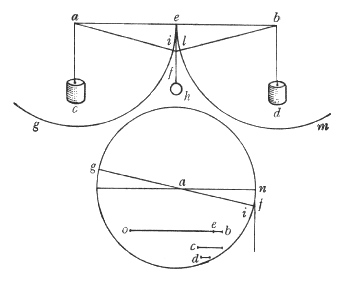
\includegraphics[width=8.75cm,height=7.05cm,keepaspectratio]{images/figura81.png} \end{center}
\end{center}

intendete per ora, questa linea \emph{ab}, passando sopra i due punti fissi e stabili \emph{a}, \emph{b}, aver nelle estremità sue pendenti, come vedete, due immensi pesi \emph{c}, \emph{d}, li quali, tirandola con grandissima forza, la facciano star veramente tesa dirittamente, essendo essa una semplice linea, senza veruna gravità. Or qui vi soggiungo e dico, che se dal mezzo di quella, che sia il punto \emph{e}, voi sospenderete qualsivoglia piccolo peso, quale sia questo \emph{h}, la linea \emph{ab} cederà, ed inclinandosi verso il punto \emph{f}, ed in consequenza allungandosi, costringerà i due gravissimi pesi \emph{c}, \emph{d} a salir in alto: il che in tal guisa vi dimostro. Intorno a i due punti \emph{a}, \emph{b}, come centri, descrivo 2 quadranti, \emph{eig}, \emph{elm}; ed essendo che li due semidiametri \emph{ai}, \emph{bl} sono eguali alli due \emph{ae}, \emph{eb}, gli avanzi \emph{fi}, \emph{fl} saranno le quantità de gli allungamenti delle parti \emph{af}, \emph{fb} sopra le \emph{ae}, \emph{eb}, ed in conseguenza determinano le salite de i pesi \emph{c}, \emph{d}, tutta volta però che il peso \emph{h} avesse auto facoltà di calare in \emph{f}: il che allora potrebbe seguire, quando la linea \emph{ef}, che è la quantità della scesa di esso peso \emph{h}, avesse maggior proporzione alla linea \emph{fi}, che determina la salita de i due pesi \emph{c}, \emph{d} che non ha la gravità di amendue essi pesi alla gravità del peso \emph{h}. Ma questo necessariamente avverrà, sia pur quanto si voglia massima la gravità de i pesi \emph{c}, \emph{d}, e minima quella dell'\emph{h}: imperò che non è sì grande l'eccesso de i pesi \emph{c}, \emph{d} sopra 'l peso \emph{h}, che maggiore non possa essere a proporzione l'eccesso della tangente \emph{ef} sopra la parte della segante \emph{fi}. Il che proveremo così. Sia il cerchio, il cui diametro \emph{gai}: e qual proporzione ha la gravità de i pesi \emph{c}, \emph{d} alla gravità di \emph{h}, tale la abbia la linea \emph{bo} ad un'altra, che sia \emph{c}, della quale sia minore la \emph{d}, sì che maggior proporzione arà la \emph{bo} alla \emph{d} che alla \emph{c}. Prendasi delle due \emph{ob}, \emph{d} la terza proporzionale \emph{be}, e come \emph{oe} ad \emph{eb}, così si faccia il diametro \emph{gi} (prolungandolo) all'\emph{if}, e dal termine \emph{f} tirisi la tangente \emph{fn}; e perché si è fatto, come \emph{oe} ad \emph{eb}, così \emph{gi} ad \emph{if}, sarà, componendo, come \emph{ob} a \emph{be}, così \emph{gf} ad \emph{fi}: ma tra \emph{ob} e \emph{be} media la \emph{d}, e tra \emph{gf}, \emph{fi} media la \emph{nf}: adunque \emph{nf} alla \emph{fi} ha la medesima proporzione che la \emph{ob} alla \emph{d}, la qual proporzione è maggiore di quella de i pesi \emph{c}, \emph{d} al peso \emph{h}. Avendo dunque maggior proporzione la scesa o velocità del peso \emph{h} alla salita o velocità dei pesi \emph{c}, \emph{d}, che non ha la gravità di essi pesi \emph{c}, \emph{d} alla gravità del peso \emph{h}; resta manifesto che il peso \emph{h} descenderà, cioè la linea \emph{ab} partirà dalla rettitudine orizontale. E quel che avviene alla retta \emph{ab} priva di gravità, mentre si attacchi in \emph{e} qualsivoglia minimo peso \emph{h}, avviene all'istessa corda \emph{ab} intesa di materia pesante, senza l'aggiunta di alcun altro grave; poiché vi si sospende il peso istesso della materia componente essa corda \emph{ab}.

\speaker{Simp.} Io resto satisfatto a pieno: però potrà il Sig. Salviati, conforme alla promessa, esplicarci qual sia l'utilità che da simile catenella si può ritrarre, e, dopo questo, arrecarci quelle specolazioni che dal nostro Accademico sono state fatte intorno alla forza della percossa.

\speaker{Salv.} Assai per questo giorno ci siamo occupati nelle contemplazioni passate: l'ora, che non poco è tarda, non ci basterebbe a gran segno per disbrigarci dalle nominate materie; però differiremo il congresso ad altro tempo più opportuno.

\speaker{Sagr.} Concorro col parere di V. S., perché da diversi ragionamenti auti con amici intrinseci del nostro Accademico ho ritratto, questa materia della forza della percossa essere oscurissima, né di quella sin ora esserne, da chiunque ne ha trattato, penetrato i suoi ricetti, pieni di tenebre ed alieni in tutto e per tutto dalle prime immaginazioni umane; e tra le conclusioni sentite profferire me ne resta in fantasia una stravagantissima, cioè che la forza della percossa è interminata, per non dir infinita. Aspetteremo dunque la commodità del Sig. Salviati. Ma intanto dicami che materie sono queste, che si veggono scritte dopo il trattato de i proietti.

\speaker{Salv.} Queste sono alcune proposizioni attenenti al centro di gravità de i solidi, le quali in sua gioventù andò ritrovando il nostro Accademico, parendogli che quello che in tal maniera aveva scritto Federigo Comandino non mancasse di qualche imperfezzione. Credette dunque con queste proposizioni, che qui vedete scritte, poter supplire a quello che si desiderava nel libro del Comandino; ed applicossi a questa contemplazione ad instanza dell'Illustrissimo Sig. Marchese Guid'Ubaldo Dal Monte, grandissimo matematico de' suoi tempi, come le diverse sue opere publicate ne mostrano, ed a quel Signore ne dette copia, con pensiero di andar seguitando cotal materia anco ne gli altri solidi non tocchi dal Comandino; ma incontratosi, dopo alcun tempo, nel libro del Sig. Luca Valerio, massimo geometra, e veduto come egli risolve tutta questa materia senza niente lasciar in dietro, non seguitò più avanti, ben che le aggressioni sue siano per strade molto diverse da quelle del Sig. Valerio.

\speaker{Sagr.} Sarà bene dunque che in questo tempo che s'intermette tra i nostri passati ed i futuri congressi, V. S. mi lasci nelle mani il libro, che io tra tanto anderò vedendo e studiando le proposizioni conseguentemente scrittevi.

\speaker{Salv.} Molto volentieri eseguisco la vostra domanda, e spero che V. S. prenderà gusto di tali proposizioni.


\vspace{1.5em}\begin{center}\large\itshape Finisce la quarta Giornata\end{center}

\appendix
\chapter*{Appendice\\{\normalsize\itshape Teoremi e dimostrazioni intorno al centro di gravità dei solidi}}
\addcontentsline{toc}{chapter}{Appendice — Intorno al centro di gravità dei solidi}
\markboth{Appendice}{Centro di gravità dei solidi}
\textbf{POSTULATO}\\ Dati dei pesi eguali similmente disposti in bilance diverse, postuliamo che, se il centro di gravità del composto degli uni divide la [relativa] bilancia secondo una certa proporzione, anche il centro di gravità del composto degli altri divide la [rispettiva] bilancia secondo la medesima proporzione.

\textbf{LEMMA}


\begin{center}
\begin{center} 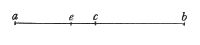
\includegraphics[width=5.00cm,height=1.12cm,keepaspectratio]{images/figura82.png} \end{center}
\end{center}

La linea \emph{ab} sia intersecata a metà in \emph{c}, e la metà \emph{ac} sia divisa in \emph{e}; sì che, qual è la proporzione che \emph{be} ha ad \emph{ea}, tale sia quella che \emph{ae} ha ad \emph{ec}. Dico, che la \emph{be} è doppia della stessa \emph{ea}. Infatti, poiché, come \emph{be} sta ad \emph{ea}, così \emph{ea} sta ad \emph{ec}, componendo e permutando, avremo che, come \emph{ba} sta ad \emph{ac}, così \emph{ae} sta ad \emph{ec}; ma come \emph{ae} sta ad \emph{ec}, cioè come \emph{ba} ad \emph{ac}, così \emph{be} sta ad \emph{ea}: perciò \emph{be} è doppia della stessa \emph{ea}.

Ciò posto, si dimostra che: Se un numero qualsiasi di grandezze, che si eccedono egualmente e i cui eccessi sono eguali alla minima di esse, vengono disposte su una bilancia in modo che pendano a distanze eguali, il centro di gravità di tutte [le grandezze] divide la bilancia in modo tale che la parte verso le [grandezze] minori è doppia dell'altra.


\begin{center}
\begin{center} 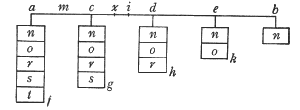
\includegraphics[width=7.50cm,height=2.75cm,keepaspectratio]{images/figura83.png} \end{center}
\end{center}

Pertanto, sulla bilancia \emph{ab}, a distanze eguali, pendano, in numero qualsiasi, le grandezze \emph{f}, \emph{g}, \emph{h}, \emph{k}, \emph{n}, le quali siano come si è detto; e la minima di esse sia \emph{n}; inoltre siano \emph{a}, \emph{c}, \emph{d}, \emph{e}, \emph{b}, i punti di sospensione, e sia \emph{x} il centro di gravità di tutte le grandezze così disposte. Bisogna mostrare che la parte \emph{bx} della bilancia, verso le grandezze minori, è doppia dell'altra [parte] \emph{xa}.

Si divida la bilancia a metà nel punto \emph{d}, che necessariamente cadrà o in qualcuno dei punti di sospensione, o nel punto di mezzo tra due sospensioni; ora, le altre distanze fra le sospensioni comprese tra \emph{a} e \emph{d} siano tutte divise a metà nei punti \emph{m} e \emph{i}; le grandezze, poi, vengono tutte divise in parti eguali alla \emph{n}; il numero delle parti della \emph{f} sarà allora eguale al numero delle grandezze che pendono dalla bilancia; le parti della \emph{g}, invece, saranno una di meno, e così per tutte le altre. Le parti della \emph{f} siano, pertanto, \emph{n}, \emph{o}, \emph{r}, \emph{s}, \emph{t}; quelle della \emph{g} [siano] \emph{n}, \emph{o}, \emph{r}, \emph{s}; quelle della \emph{h} [siano] \emph{n}, \emph{o}, \emph{r}; infine, le parti della \emph{k} siano \emph{n} e \emph{o}: tutte le parti [\emph{cioè la loro somma}] segnate da \emph{n} saranno eguali alla \emph{f}; tutte quelle segnate da \emph{o}, saranno eguali alla \emph{g}; quelle segnate da \emph{r}, saranno eguali alla \emph{h}; quelle segnate da \emph{s}, lo saranno alla \emph{k}; infine la grandezza \emph{t} è eguale alla \emph{n}. Poiché, dunque, tutte le grandezze segnate da \emph{n} sono tra di loro eguali, il punto del loro equilibrio sarà in \emph{d}, che divide a metà la bilancia \emph{ab}; per la medesima ragione, di tutte le grandezze segnate da \emph{o} il punto di equilibrio è in \emph{i}; di quelle segnate da \emph{r} è in \emph{c}; e quelle segnate da \emph{s}, hanno il loro punto di equilibrio in \emph{m}; infine \emph{t} è appesa in \emph{a}. Pertanto, sulla bilancia \emph{ab}, a distanze eguali \emph{d}, \emph{i}, \emph{c}, \emph{m}, \emph{a}, sono appese grandezze che si eccedono egualmente e il cui eccesso è eguale alla minima: ma la massima, che risulta composta di tutte le \emph{n}, pende da \emph{d}; la minima, invece, cioè \emph{t}, pende da \emph{a}; e tutte le altre sono disposte ordinatamente. V'è, inoltre, un'altra bilancia \emph{ab}, sulla quale sono disposte nel medesimo ordine altre grandezze, eguali alle predette in numero e in grandezza: perciò le bilance \emph{ab} e \emph{ad} verranno divise dai centri [di gravità] del composto di tutte le grandezze secondo la medesima proporzione. Ma il centro di gravità delle suddette grandezze è \emph{x}; perciò \emph{x} divide le bilance \emph{ba} e \emph{ad} secondo la medesima proporzione, in modo che, come \emph{bx} sta a \emph{xa} così \emph{xa} stia a \emph{xd}; perciò \emph{bx} è doppia di \emph{xa}, per il lemma posto sopra. Il che è quello che si doveva provare.

Se in un conoide parabolico viene inscritta una figura e se ne circoscrive un'altra, [costituite] da cilindri aventi eguale altezza, e si divide l'asse del detto conoide in modo che la parte verso il vertice sia doppia della parte verso la base; il centro di gravità della figura inscritta sarà più vicino del detto punto di divisione alla base della porzione [ossia del conoide]; il centro di gravità della figura circoscritta, invece, sarà più lontano del medesimo punto dalla base del conoide; e la distanza di ciascuno dei due centri da tale punto sarà eguale alla linea, che sia la sesta parte dell'altezza di uno dei cilindri da cui sono costituite le figure.


\begin{center}
\begin{center} 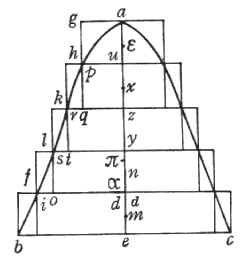
\includegraphics[width=6.25cm,height=6.68cm,keepaspectratio]{images/figura84.png} \end{center}
\end{center}

Siano, pertanto, un conoide parabolico e figure tali, quali si sono dette: l'una sia inscritta, l'altra circoscritta; l'asse del conoide, il quale sia \emph{ae}, venga diviso nel punto \emph{n} in modo che \emph{an} sia doppia di \emph{ne}. Bisogna mostrare che il centro di gravità della figura inscritta si trova sulla linea \emph{ne}, mentre il centro di quella circoscritta si trova sulla \emph{an}. Le figure così disposte vengano intersecate da un piano [passante] per l'asse, e la sezione della parabola [\emph{ossia del conoide parabolico}] sia \emph{bac}: l'intersezione del piano secante con la base del conoide sia la linea \emph{bc}; le sezioni dei cilindri siano figure rettangolari: come risulta nel disegno. Ora, il primo dei cilindri inscritti, il cui asse è \emph{de}, rispetto al cilindro, il cui asse è \emph{dy}, ha la medesima proporzione che il quadrato \emph{id} al quadrato \emph{sy}, cioè che da \emph{da} ad \emph{ay}; inoltre, il cilindro, il cui asse è \emph{dy}, sta al cilindro \emph{yz}, come il quadrato di \emph{sy} sta al quadrato di \emph{rz}, cioè come \emph{ya} sta ad \emph{az}; e, per la stessa ragione, il cilindro, il cui asse è \emph{zy}, sta a quello, il cui asse è \emph{zu}, come \emph{za} sta ad \emph{au}. Dunque, i suddetti cilindri stanno tra di loro come le linee \emph{da}, \emph{ay}, \emph{za}, \emph{au}: ma queste linee sono tra loro egualmente eccedenti e il loro eccesso è eguale alla minima, in modo che \emph{az} risulta doppia di \emph{au}, mentre \emph{ay} ne risulta tripla, e \emph{da} quadrupla. I suddetti cilindri sono, dunque, grandezze egualmente eccedentisi l'una l'altra, i cui eccessi sono eguali alla minima di esse; inoltre la linea \emph{xm} è quella, sulla quale esse sono appese a distanze eguali (infatti ciascun cilindro ha il centro di gravità nel mezzo del proprio asse): perciò, per le cose sopra dimostrate, il centro di gravità della grandezza composta da tutte [le grandezze date] dividerà la linea \emph{xm} in modo che la parte verso \emph{x} sia doppia dell'altra. Si faccia, dunque, la divisione, e \emph{xa}sia doppia di a \emph{m}: dunque, a è il centro di gravità della figura inscritta. Si divida la \emph{au} a metà in e ; e \emph{x} sarà doppia della \emph{me}: ma \emph{xa}è doppia della a \emph{m}, perciò e \emph{e} è tripla della \emph{ea}. Ma \emph{ae} è tripla della \emph{en}: risulta, dunque, che \emph{en} è maggiore della \emph{ea}, e perciò a , che è il centro di gravità della figura inscritta, è più vicino di \emph{n} alla base del conoide. Poiché, come \emph{ae} sta ad \emph{en}, così la parte tolta e \emph{e} sta alla parte tolta \emph{ea}, si avrà che anche la parte rimanente starà all'altra parte rimanente, cioè \emph{ae}ad \emph{na}, come \emph{ae} sta ad \emph{en}. Dunque, a \emph{n} è la terza parte di \emph{ae}e la sesta parte di \emph{au}. Nel medesimo modo si dimostra poi che i cilindri della figura circoscritta si eccedono egualmente, che gli eccessi sono eguali al cilindro minimo, e che i loro centri di gravità si trovano sulla linea e \emph{m} a distanze eguali. Se, pertanto, si divide e \emph{m} in p , in modo che e p sia doppia della rimanente p \emph{m}, p sarà il centro di gravità dell'intera grandezza circoscritta: inoltre, poiché e p è doppia di p \emph{m}, mentre \emph{ae}è minore del doppio di \emph{em} (poiché le è eguale), l'intera \emph{ae} risulterà minore del triplo della \emph{ep}; perciò \emph{ep}sarà maggiore della \emph{en}. Inoltre, essendo la e \emph{m} tripla della \emph{mp}ed essendo [la somma di] \emph{me} col doppio di e \emph{a} parimenti tripla della \emph{me}, allora l'intera \emph{ae}, insieme con la \emph{ae}, sarà tripla della \emph{ep}. Ma \emph{ae} è tripla della \emph{en}; perciò la rimanente \emph{ae}sarà tripla della rimanente p \emph{n}. Pertanto \emph{np}è la sesta parte della \emph{au}. Questo è appunto quanto si doveva dimostrare.

Da ciò è manifesto che in un conoide parabolico è possibile inscrivere una figura e circoscriverne un'altra, in modo che i loro centri di gravità distino dal punto \emph{n} meno di qualunque linea data. Se, infatti, data una linea, ne prendiamo un'altra sei volte maggiore, e se facciamo gli assi dei cilindri, dai quali sono costituite le figure, minori della linea così presa; allora le linee che si trovano fra il centro di gravità di ciascuna di queste figure e il punto \emph{n}, saranno minori della linea data.

\textbf{ALTRA DIMOSTRAZIONE DELLO STESSO}


\begin{center}
\begin{center} 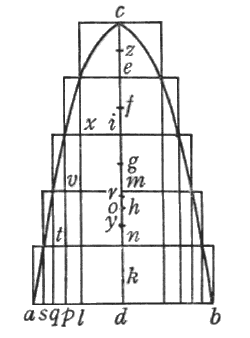
\includegraphics[width=6.25cm,height=8.45cm,keepaspectratio]{images/figura85.png} \end{center}
\end{center}

L'asse di un conoide, che sia \emph{cd}, venga diviso in \emph{o} in modo che \emph{co} sia doppia di \emph{od}. Bisogna mostrare che il centro di gravità della figura inscritta si trova sulla linea \emph{od}, mentre il centro di quella circoscritta si trova sulla \emph{co}. Le figure siano intersecate da un piano [passante] per l'asse e per \emph{c}, come si è detto. Ordunque, poiché i cilindri \emph{sn}, \emph{tm}, \emph{vi}, \emph{xe} stanno tra loro come i quadrati delle linee \emph{sd}, \emph{tn}, \emph{vm}, \emph{xi}; [poiché] d'altra parte questi [quadrati] stanno tra di loro come le linee \emph{nc}, \emph{cm}, \emph{ci}, \emph{ce}; [poiché] inoltre queste [linee] si eccedono egualmente e gli eccessi sono eguali alla minima, cioè alla \emph{ce}; e [poiché] il cilindro \emph{tm} è eguale al cilindro \emph{qn}, mentre il cilindro \emph{vi} è eguale al cilindro \emph{pn}, e il cilindro \emph{xe} è eguale al cilindro \emph{ln}; dunque, i cilindri \emph{sn}, \emph{qn}, \emph{pn}, \emph{ln} si eccedono egualmente e gli eccessi sono eguali al minimo di essi, cioè al cilindro \emph{ln}. Ma l'eccesso del cilindro \emph{sn} sul cilindro \emph{qn} è un anello, la cui altezza è \emph{qt}, cioè \emph{nd}, e la cui larghezza è \emph{sq}; l'eccesso del cilindro \emph{qn} sul cilindro \emph{pn} è un anello, la cui larghezza è \emph{qp}; infine l'eccesso del cilindro \emph{pn} sul cilindro \emph{ln} è un anello, la cui larghezza è \emph{pl}. Perciò i suddetti anelli \emph{sq}, \emph{qp}, \emph{pl} sono eguali [equivalenti] tra di loro e al cilindro \emph{ln}. L'anello \emph{st} è pertanto eguale al cilindro \emph{xe}; l'anello \emph{qv}, doppio dell'anello \emph{st}, è eguale al cilindro \emph{vi}, il quale è similmente doppio del cilindro \emph{xe}; e per la stessa ragione, l'anello \emph{px} sarà eguale al cilindro \emph{tm}, e il cilindro \emph{le} al cilindro \emph{sn}. Pertanto, sulla bilancia \emph{kf}, la quale unisce i punti medi delle rette \emph{ei} e \emph{dn} ed è intersecata in parti eguali nei punti \emph{h} e \emph{g}, si trovano delle grandezze, cioè i cilindri \emph{sn}, \emph{tm}, \emph{vi}, \emph{xe}; e il centro di gravità del primo cilindro è \emph{k}, quello del secondo è \emph{h}, quello del terzo è \emph{g}, e quello del quarto è \emph{f}. Ma abbiamo anche un'altra bilancia \emph{mk}, che è la metà della \emph{fk}, e che è divisa da altrettanti punti in parti eguali, cioè \emph{mh}, \emph{hn}, \emph{nk}; su di essa si trovano altre grandezze, le quali sono eguali in numero e grandezza a quelle che si trovano sulla bilancia \emph{fk}, e hanno i [rispettivi] centri di gravità nei punti \emph{m}, \emph{h}, \emph{n}, \emph{k}, e sono disposte nel medesimo ordine. Il cilindro \emph{le} ha infatti il centro di gravità in \emph{m}, ed è eguale al cilindro \emph{sn}, che ha il centro di gravità in \emph{k}; l'anello \emph{px} ha il centro di gravità in \emph{h}, ed è eguale al cilindro \emph{tm}, il cui centro di gravità è \emph{h}; l'anello \emph{qv}, avente il centro di gravità in \emph{n}, è eguale al cilindro \emph{vi}, il cui centro è \emph{g}; infine l'anello \emph{st}, avente il centro di gravità in \emph{k}, è eguale al cilindro \emph{xe}, il cui centro è \emph{f}. Pertanto, il centro di gravità delle suddette grandezze divide la bilancia secondo la medesima proporzione: ma il loro centro è unico, e perciò è un qualche punto comune ad entrambe le bilance, il quale [punto] sia \emph{y}. Pertanto \emph{fy} starà a \emph{yk} come \emph{ky} a \emph{ym}; dunque, \emph{fy} è doppia della \emph{yk}; e divisa la \emph{ce} a metà in \emph{z}, \emph{zf} sarà doppia di \emph{kd}, e di conseguenza \emph{zd} sarà tripla della \emph{dy}. Ma della retta \emph{do} è tripla la \emph{cd}: dunque, la retta \emph{do} è maggiore della \emph{dy}; e perciò il centro di gravità \emph{y} della figura inscritta è più vicino del punto \emph{o} alla base. E poiché, come \emph{cd} sta a \emph{do}, così la parte tolta \emph{zd} sta alla parte tolta \emph{dy}, allora anche la parte rimanente \emph{cz} starà alla parte rimanente \emph{yo} come \emph{cd} sta a \emph{do}: cioè \emph{yo} sarà la terza parte della \emph{cz}, cioè la sesta parte della \emph{ce}. Con identico procedimento mostreremo, d'altra parte, che i cilindri della figura circoscritta si eccedono egualmente, che gli eccessi sono eguali al cilindro minimo, e che i loro centri di gravità sono situati sulla bilancia \emph{kz} a distanze eguali; inoltre [dimostreremo] parimenti che anelli eguali ai medesimi cilindri sono similmente disposti sull'altra bilancia \emph{kg}, che è la metà della bilancia \emph{kz}; e che, perciò, il centro di gravità della figura circoscritta, il quale sia \emph{r}, divide le bilance in modo che \emph{zr} stia ad \emph{rk}, come \emph{kr} sta ad \emph{rg}. Dunque, \emph{zr} sarà doppia della \emph{rk}; ma \emph{cz} sarà eguale alla retta \emph{kd}, e non doppia: l'intera \emph{cd} sarà allora minore del triplo della \emph{dr}; perciò la retta \emph{dr} è maggiore della \emph{do}: ovverossia, il centro di gravità della figura circoscritta è più distante del punto \emph{o} dalla base. E poiché \emph{zk} è tripla della \emph{kr}, e [la somma di] \emph{kd} col doppio di \emph{zc} è tripla di \emph{kd}, l'intera \emph{cd}, insieme con \emph{cz}, sarà tripla della \emph{dr}. Ma \emph{cd} è tripla della \emph{do}: perciò la parte rimanente \emph{cz} sarà tripla dell'altra parte rimanente \emph{ro}: cioè \emph{or} è la sesta parte della \emph{ec}. Che è quello che ci eravamo proposti.

Fatte queste dimostrazioni iniziali, si dimostra ora che il centro di gravità di un conoide parabolico divide l'asse in modo tale che la parte verso il vertice è doppia della rimanente parte verso la base.


\begin{center}
\begin{center} 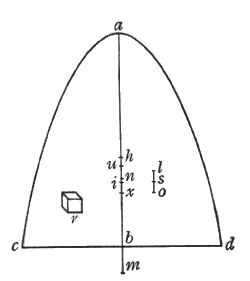
\includegraphics[width=6.25cm,height=7.03cm,keepaspectratio]{images/figura86.png} \end{center}
\end{center}

Sia un conoide parabolico, il cui asse \emph{ab} venga diviso in \emph{n} in modo che \emph{an} sia doppia di \emph{nb}. Bisogna mostrare che il centro di gravità del conoide è il punto \emph{n}. Infatti, se non è \emph{n}, si troverà o sotto o sopra di esso. In primo luogo [immaginiamo che] si trovi sotto, e sia esso \emph{x}: si ponga a parte la linea \emph{lo}, eguale alla \emph{nx}, e la si divida a caso in \emph{s}; e qual è la proporzione che [la somma di] ambedue le \emph{bx} e \emph{os} ha rispetto a \emph{os}, tale sia anche la proporzione che il conoide ha rispetto al solido \emph{r}: si inscriva nel conoide una figura [costituita] da cilindri aventi eguale altezza, in modo che la linea compresa tra il centro di gravità di essa [figura] e il punto \emph{n} sia minore della linea \emph{ls}, e l'eccesso, per il quale [quella figura] viene superata dal conoide, sia minore del solido \emph{r}. Che poi ciò sia possibile, è manifesto. Sia pertanto inscritta [la figura], il cui centro di gravità sia \emph{i}: sarà allora \emph{ix} maggiore di \emph{so}; poiché abbiamo che, come [la somma di] \emph{xb} con \emph{so} sta ad \emph{so}, così il conoide sta ad \emph{r} (ma \emph{r} è maggiore dell'eccesso per il quale il conoide supera la figura inscritta), la proporzione del conoide al suddetto eccesso sarà maggiore della proporzione che [la somma di] ambedue le \emph{bx} e \emph{os} ha rispetto ad \emph{so}: scomponendo, la figura inscritta avrà, rispetto al suddetto eccesso, una proporzione maggiore della proporzione di \emph{bx} ad \emph{so}. Ma la proporzione di \emph{bx} a \emph{xi} è ancora minore di quella che [la medesima \emph{bx}] ha ad \emph{so}: la figura inscritta avrà, pertanto, rispetto alle rimanenti porzioni, una proporzione molto maggiore di quella che \emph{bx} ha ad \emph{xi}. Pertanto, quale è la proporzione che la figura inscritta ha rispetto alle rimanenti porzioni, tale sarà anche la proporzione di un'altra linea qualsiasi a \emph{xi}; [linea] che risulterà necessariamente maggiore di \emph{bx}. Sia essa, pertanto, \emph{mx}. Abbiamo così in \emph{x} il centro di gravità del conoide, e in \emph{i} quello della figura inscritta: dunque, il centro di gravità delle rimanenti porzioni, per le quali il conoide eccede la figura inscritta, si troverà sulla linea \emph{xm}, e precisamente in quel punto che determinerebbe su di essa una linea tale, che il rapporto di quest'ultima a \emph{xi} sia eguale alla proporzione che la figura inscritta ha rispetto all'eccesso, per il quale è superata dal conoide. Ma si è mostrato che tale proporzione è appunto quella che \emph{mx} ha a \emph{xi}: sarà dunque \emph{m} il centro di gravità delle porzioni, per le quali il conoide eccede la figura inscritta. Il che non è certamente possibile: infatti, se per \emph{m} si conduce un piano equidistante dalla base del conoide, tutte le porzioni suddette si troveranno da una stessa parte, e non saranno divise da esso. Pertanto, il centro di gravità del conoide non si trova al di sotto del punto \emph{n}. Ma nemmeno [si trova] sopra. Infatti, qualora sia possibile, [immaginiamo che] esso sia \emph{h}; e, di nuovo, come sopra, si ponga a parte la linea \emph{lo} eguale alla \emph{hn}, e la si divida a caso in \emph{s}; e quale è la proporzione che [la somma di] entrambe le \emph{bn} ed \emph{so} ha ad \emph{sl}, tale sia anche la proporzione che il conoide ha ad \emph{r}; si circoscriva al conoide una figura [costituita] da cilindri nel modo che si è detto, la quale sia eccedente [rispetto al conoide] per una quantità minore del solido \emph{r}; e la linea [compresa] tra il centro di gravità della figura circoscritta e il punto \emph{n} sia minore di \emph{so}: la restante \emph{uh} sarà maggiore di \emph{ls}; e poiché abbiamo che, come [la somma di] entrambe le \emph{bn} e \emph{os} sta ad \emph{sl}, così il conoide sta ad \emph{r} (ma \emph{r} è maggiore dell'eccesso, per il quale il conoide è superato dalla figura circoscritta), dunque [la somma di] \emph{bn} e \emph{os} avrà rispetto ad \emph{sl} una proporzione minore di quella che il conoide ha rispetto al suddetto eccesso. Ma \emph{bu} è minore [della somma] di \emph{bn} e \emph{os}; \emph{uh}, invece, è maggiore di \emph{sl}: pertanto il conoide avrà rispetto alle suddette porzioni una proporzione molto maggiore di quella che \emph{bu} ha ad \emph{uh}. Pertanto, quale è la proporzione che il conoide ha rispetto a quelle medesime porzioni, tale sarà pure la proporzione che una linea maggiore della \emph{bu} avrà rispetto alla \emph{uh}. L'abbia, dunque, e sia essa \emph{mu}; poiché il centro di gravità della figura circoscritta è \emph{u}, e il centro di gravità del conoide è \emph{h}, e poiché abbiamo inoltre che, come il conoide sta alle porzioni rimanenti, così \emph{mu} sta a \emph{uh}, sarà allora \emph{m} il centro di gravità di quelle porzioni rimanenti: il che è similmente impossibile. Il centro di gravità del conoide non si trova dunque al di sopra del punto \emph{n}: ma si è dimostrato che non si trova neppure al di sotto: resta dunque che esso debba necessariamente trovarsi proprio in \emph{n}. E col medesimo procedimento ciò si dimostrerà di un conoide intersecato da un piano non perpendicolare all'asse. In altre parole, ma è la stessa cosa, come risulta nel [teorema] seguente, il centro di gravità di un conoide parabolico va a cadere tra il centro della figura circoscritta e il centro di quella inscritta.


\begin{center}
\begin{center} 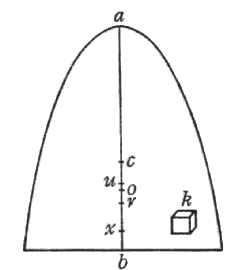
\includegraphics[width=6.25cm,height=6.75cm,keepaspectratio]{images/figura87.png} \end{center}
\end{center}

Sia un conoide avente asse \emph{ab}: il centro della figura circoscritta sia \emph{c}, e quello della figura inscritta sia \emph{o}. Dico, che il centro del conoide si trova tra i punti \emph{c} e \emph{o}. Infatti, se ciò non fosse, dovrà trovarsi o al di sopra, o al di sotto, o in uno di essi. Sia al di sotto, ad esempio in \emph{r}: poiché \emph{r} è il centro di gravità dell'intero conoide e \emph{o} il centro di gravità della figura inscritta, dunque il centro di gravità di tutte le altre porzioni, per le quali la figura inscritta è superata dal conoide, si troverà sul prolungamento della linea \emph{or} dalla parte di \emph{r}, e precisamente in quel punto che delimita [questo prolungamento] in modo che, quale è la proporzione delle dette porzioni alla figura inscritta, tale sia anche la proporzione che la linea \emph{or} ha rispetto alla linea compresa tra \emph{r} e quel punto. Questa proporzione sia quella che \emph{or} ha ad \emph{rx}. Pertanto \emph{x} andrà a cadere o al di fuori del conoide, o al di dentro, oppure sulla base stessa. Sia [l'ipotesi] che esso cada al di fuori, sia [quella] che esso cada sulla base, risultano già manifestamente assurde. [Supponiamo che] vada a cadere all'interno: poiché \emph{xr} sta ad \emph{ro}, come la figura inscritta sta all'eccesso, per il quale essa è superata dal conoide, poniamo che, quale è la proporzione di \emph{br} ad \emph{ro}, tale sia anche quella che la figura inscritta ha rispetto al solido \emph{k}, il quale dovrà essere necessariamente minore del suddetto eccesso; si inscriva poi un'altra figura, la quale sia superata dal conoide per un eccesso minore di \emph{k}: il suo centro di gravità cadrà tra \emph{o} e \emph{c}. Sia esso \emph{u}: poiché la prima figura sta a \emph{k} come \emph{br} sta ad \emph{ro}, e poiché, d'altra parte, la seconda figura, il cui centro é \emph{u}, è maggiore della prima ed è superata dal conoide per un eccesso minore di \emph{k}, si avrà allora che, quale è la proporzione che la seconda figura ha rispetto all'eccesso, per il quale essa è superata dal conoide, tale è anche la proporzione che una linea maggiore della \emph{br} ha rispetto alla linea \emph{ru}. Ma il centro di gravità del conoide è \emph{r}, mentre quello della figura inscritta è \emph{u}: dunque, il centro di gravità delle rimanenti porzioni si troverà al di fuori del conoide, al di sotto di \emph{b}; il che è impossibile. E col medesimo procedimento si dimostrerà che il centro di gravità del medesimo conoide non si trova sulla linea \emph{ca}. Che poi esso non sia né l'uno né l'altro dei due punti \emph{c} e \emph{o}, ciò è manifesto. Infatti, qualora supponessimo ciò, descritte [due] altre figure, tali che quella inscritta sia maggiore della figura il cui centro è \emph{o}, e quella circoscritta sia minore della figura il cui centro è \emph{c}, il centro di gravità del conoide andrebbe a cadere fuori del centro di gravità di tali figure: il che è impossibile, come abbiamo testé concluso. Ne consegue, dunque, che esso si trova compreso tra il centro della figura circoscritta e quello della figura inscritta. Se è così, dovrà trovarsi necessariamente in quel punto che divide l'asse in modo che la parte verso il vertice sia doppia della rimanente. Infatti, poiché si possono inscrivere e circoscrivere figure tali, che le linee comprese tra il loro centro di gravità e il punto suddetto siano minori di qualunque linea data, chi affermasse cosa diversa verrebbe condotto a questo assurdo: che, cioè, il centro del conoide non si trovi tra i centri della figura inscritta e di quella circoscritta.

Se vi sono tre linee proporzionali, e si prende un'altra linea qualsiasi, tale che la proporzione che essa ha rispetto ai due terzi dell'eccesso, per il quale la massima supera la media, sia eguale alla proporzione che la minima ha rispetto all'eccesso, per il quale la massima supera la minima; se inoltre si prende ancora un'altra linea tale, che la proporzione che essa ha rispetto all'eccesso, per il quale la massima supera la media, sia eguale alla proporzione che la linea, composta dalla massima e dal doppio della media, ha rispetto alla linea composta dal triplo della massima e della media; [la somma di] ambedue le linee prese insieme sarà [eguale al] la terza parte della massima tra le linee proporzionali.


\begin{center}
\begin{center} 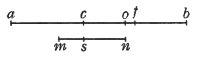
\includegraphics[width=5.00cm,height=1.45cm,keepaspectratio]{images/figura88.png} \end{center}
\end{center}

Siano tre linee proporzionali \emph{ab}, \emph{bc}, \emph{bf}: e quale è la proporzione che \emph{bf} ha ad \emph{af}, tale sia anche quella che \emph{ms} ha rispetto ai due terzi della \emph{ca}; inoltre, quale è la proporzione che la linea composta da \emph{ab} e dal doppio di \emph{bc} ha rispetto alla linea composta dal triplo di ambedue le \emph{ab} e \emph{bc}, tale sia anche la proporzione che un'altra linea, cioè \emph{sn}, ha ad \emph{ac}. Bisogna dimostrare che \emph{mn} è la terza parte della \emph{ab}. Pertanto, poiché \emph{ab}, \emph{bc}, \emph{bf} sono proporzionali, anche \emph{ac} e \emph{cf} si troveranno nel medesimo rapporto: perciò, come \emph{ab} sta a \emph{bc}, così \emph{ac} sta \emph{cf}; e come il triplo di \emph{ab} al triplo di \emph{bc}, così \emph{ac} a \emph{cf}. Pertanto, quale è la proporzione che [la somma del] triplo di \emph{ab} col triplo di \emph{bc} ha rispetto al triplo di \emph{cb}, tale sarà anche la proporzione che \emph{ac} ha a una linea minore della \emph{cf}. Sia essa \emph{co}. Perciò, componendo e per conversione della proporzione [\emph{invertendo}], \emph{oa} avrà ad \emph{ac} la medesima proporzione che [la somma del] triplo di \emph{ab} col sestuplo di \emph{bc} ha rispetto al [la somma del] triplo di \emph{ab} col triplo di \emph{bc}: ma \emph{ac} ha ad \emph{sn} la medesima proporzione che [la somma del] triplo di \emph{ab} col triplo di \emph{bc} ha rispetto al [la somma di] \emph{ab} col doppio di \emph{bc}: \emph{ex aequali}, dunque, \emph{oa} avrà ad \emph{ns} la medesima proporzione che [la somma del] triplo di \emph{ab} col sestuplo di \emph{bc} ha rispetto al [la somma di] \emph{ab} col doppio di \emph{bc}. Ora, [la somma del] triplo di \emph{ab} col sestuplo di \emph{bc} è eguale a tre volte [la somma di] \emph{ab} col doppio di \emph{bc}: dunque, \emph{ao} è tripla di \emph{sn}.

Inoltre, poiché \emph{oc} sta a \emph{ca} come il triplo di \emph{cb} sta alla somma del triplo di \emph{ab} col triplo di \emph{cb}; e poiché come \emph{ca} sta a \emph{cf}, così il triplo di \emph{ab} al triplo di \emph{bc}; dunque, \emph{ex aequali}, in proporzione perturbata, si avrà che, come \emph{oc} sta a \emph{cf}, così il triplo di \emph{ab} sta alla somma del triplo di \emph{ab} col triplo di \emph{bc}, e, per conversione della proporzione, come \emph{of} sta ad \emph{fc}, così il triplo di \emph{bc} sta alla somma del triplo di \emph{ab} col triplo di \emph{bc}. Ma come \emph{cf} sta ad \emph{fb}, così \emph{ac} sta a \emph{cb}, e il triplo di \emph{ac} al triplo di \emph{bc}; \emph{ex aequali}, dunque, in proporzione perturbata, si avrà che, come \emph{of} sta ad \emph{fb}, così il triplo di \emph{ac} sta al triplo di ambedue le \emph{ab} e \emph{bc} insieme. Pertanto [\emph{componendo}] l'intera \emph{ob} starà alla \emph{bf} come il sestuplo di \emph{ab} sta al triplo di ambedue le \emph{ab} e \emph{bc}; e poiché \emph{fc} e \emph{ca} stanno tra di loro nella medesima proporzione che \emph{cb} e \emph{ba}, si avrà che, come \emph{fc} sta a \emph{ca}, così \emph{bc} sta a \emph{ba}, e, componendo, come \emph{fa} sta ad \emph{ac}, così [la somma di] ambedue le \emph{ba} e \emph{bc} sta a \emph{ba}, e così il triplo sta al triplo: dunque, come \emph{fa} sta ad \emph{ac}, così la linea composta dal triplo di \emph{ba} e dal triplo di \emph{bc} sta al triplo di \emph{ab}; perciò come \emph{fa} sta ai due terzi della \emph{ac}, così la linea composta dal triplo di \emph{ba} e dal triplo di \emph{bc} sta ai due terzi del triplo di \emph{ba}, cioè al doppio di \emph{ba}. Ma come \emph{fa} sta ai due terzi della \emph{ac}, così \emph{fb} sta ad \emph{ms}; dunque, come \emph{fb} sta ad \emph{ms}, così la linea composta dal triplo di \emph{ba} e dal triplo di \emph{bc} sta al doppio di \emph{ba}. Ma come \emph{ob} sta ad \emph{fb}, così il sestuplo di \emph{ab} stava al triplo di ambedue le \emph{ab} e \emph{bc}: dunque, \emph{ex aequali}, \emph{ob} avrà ad \emph{ms} la medesima proporzione che il sestuplo di \emph{ab} al doppio di \emph{ba}; perciò \emph{ms} sarà la terza parte della \emph{ob}. Si è anche dimostrato che \emph{sn} è la terza parte di \emph{ao}: risulta dunque che \emph{mn} è, similmente, la terza parte di \emph{ab}. E ciò è quello che si doveva dimostrare.

Il centro di gravità di un qualsiasi frusto [tronco] staccato da un conoide parabolico si trova sulla linea retta che è l'asse del frusto; diviso tale asse in tre parti eguali, il centro di gravità si trova nella parte di mezzo e la divide in modo che la parte verso la base minore avrà rispetto alla parte verso la base maggiore, la medesima proporzione che la base maggiore ha rispetto alla base minore.


\begin{center}
\begin{center} 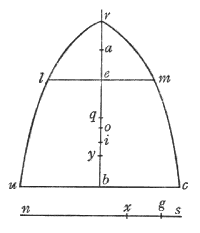
\includegraphics[width=5.00cm,height=5.83cm,keepaspectratio]{images/figura89.png} \end{center}
\end{center}

Dal conoide, il cui asse è \emph{rb}, sia staccato il solido, il cui asse è \emph{be}, e il piano secante [con cui è operata tale scissione] sia equidistante dalla base; si faccia inoltre una sezione per mezzo di un altro piano passante per l'asse perpendicolare alla base: tale sezione della parabola [\emph{sezione del conoide},\emph{la quale genera una parabola}] sia \emph{urc}; inoltre le intersezioni di quest'ultimo piano col piano secante e con la base siano [rispettivamente] le linee rette \emph{lm} ed \emph{uc}: \emph{rb} sarà il diametro di proporzione, o sarà equidistante dal diametro; \emph{lm} e \emph{uc} saranno ordinatamente applicate ad esso. Si divida, pertanto, \emph{eb} in tre parti eguali, tra le quali la parte media sia \emph{qy}; ora quest'ultima sia divisa dal punto \emph{i} in modo che, quale è la proporzione della base, il cui diametro è \emph{uc}, alla base, il cui diametro è \emph{lm}, cioè del quadrato di \emph{uc} al quadrato di \emph{lm}, tale sia anche la proporzione di \emph{qi} a \emph{iy}. Bisogna dimostrare che \emph{i} è il centro di gravità del frusto \emph{lmc}. Si ponga a parte la linea \emph{ns} eguale alla \emph{br}, e \emph{sx} sia eguale ad \emph{er}; inoltre si prenda \emph{sg} terza proporzionale delle linee \emph{ns} ed \emph{sx}; infine, quale è la proporzione che \emph{ng} ha a \emph{gs}, tale sia anche quella che la linea \emph{bq} ha rispetto a \emph{io}. Non importa che il punto \emph{o} si trovi sopra o sotto la \emph{lm}. Poiché nella sezione \emph{urc} le linee \emph{lm} e \emph{uc} sono ordinatamente applicate, si avrà che, come il quadrato di \emph{uc} sta al quadrato di \emph{lm}, così la linea \emph{br} sta alla linea \emph{re}: ma come il quadrato \emph{uc} sta al quadrato \emph{lm}, così \emph{qi} sta a \emph{iy}, e come \emph{br} sta ad \emph{re}, così \emph{ns} ad \emph{sx}; dunque, \emph{qi} sta a \emph{iy} come \emph{ns} ad \emph{sx}. Perciò, come \emph{qy} sta a \emph{yi}, così [la somma di] ambedue le \emph{ns} ed \emph{sx} starà ad \emph{sx}, e come \emph{eb} sta a \emph{yi}, così la linea composta dal triplo di \emph{ns} e dal triplo di \emph{sx} starà ad \emph{sx}: ma come \emph{eb} sta a \emph{by}, così la linea composta dal triplo di ambedue le \emph{ns} ed \emph{sx} insieme sta alla linea composta da \emph{ns} ed \emph{sx}: dunque, come \emph{eb} sta a \emph{bi}, così la linea composta dal triplo di \emph{ns} e dal triplo di \emph{sx} sta alla linea composta da \emph{ns} e dal doppio di \emph{sx}. Le tre linee \emph{ns}, \emph{sx}, \emph{gs} sono dunque proporzionali; e quale è la proporzione che \emph{sg} ha a \emph{gn}, tale è anche la proporzione che la linea presa \emph{oi} ha rispetto ai due terzi della \emph{eb}, cioè della \emph{nx}; inoltre, quale è la proporzione che la linea composta da \emph{ns} e dal doppio di \emph{sx}, ha rispetto alla linea composta dal triplo di \emph{ns} e dal triplo di \emph{sx}, tale è anche la proporzione che l'altra linea presa \emph{ib} ha rispetto a \emph{be}, cioè rispetto a \emph{nx}. Pertanto, per le cose che si sono sopra dimostrate, queste linee, prese insieme, saranno la terza parte della \emph{ns}, cioè della \emph{rb}; \emph{rb} è dunque tripla della \emph{bo}: perciò \emph{o} sarà il centro di gravità del conoide \emph{urc}. Sia poi \emph{a} il centro di gravità del conoide \emph{lrm}; dunque, il centro di gravità del frusto \emph{ulmc} si trova sulla linea \emph{ob}, e precisamente in quel punto che la delimita in modo che, quale è la proporzione che il frusto \emph{ulmc} ha rispetto alla porzione \emph{lrm}, tale sia anche la proporzione che la linea \emph{ao} ha rispetto alla linea compresa tra \emph{o} e il punto suddetto. E poiché \emph{ro} è due terzi della \emph{rb}, ed \emph{ra} i due terzi della \emph{re}; la rimanente \emph{ao} sarà i due terzi della rimanente \emph{eb}. E poiché abbiamo che, come il frusto \emph{ulmc} sta alla porzione \emph{lrm}, così \emph{ng} sta a \emph{gs}; e che, come \emph{ng} sta a \emph{gs}, così i due terzi di \emph{eb} stanno a \emph{oi}; e poiché, d'altra parte, ai due terzi di \emph{eb} è eguale la linea \emph{ao}; si avrà allora che, come il frusto \emph{ulmc} sta alla porzione \emph{lrm}, così \emph{ao} sta a \emph{oi}. Risulta, dunque, che il centro di gravità del frusto \emph{ulmc} è il punto \emph{i}, e che esso divide l'asse in modo che la parte verso la base minore sta alla parte verso la base maggiore come [la somma del] doppio della base maggiore con la base minore sta al [la somma del] doppio della minore con la maggiore. Il che è ciò che ci eravamo proposti, spiegato più elegantemente.

Se un numero qualsiasi di grandezze sono disposte tra loro [in rapporto tale] che la seconda sia superiore alla prima del doppio della prima, la terza sia superiore alla seconda del triplo della prima, la quarta sia superiore alla terza del quadruplo della prima, e così ciascuna delle grandezze che si susseguono sia superiore a quella immediatamente precedente di una grandezza multipla della prima secondo il numero [corrispondente alla posizione] che essa stessa occupa nell'ordine; se - dico - queste grandezze vengono ordinatamente appese ad eguali distanze su una bilancia, il centro di equilibrio del composto di tutte [le grandezze] dividerà la bilancia in modo che la parte verso le grandezze minori sarà tripla dell'altra [parte].


\begin{center}
\begin{center} 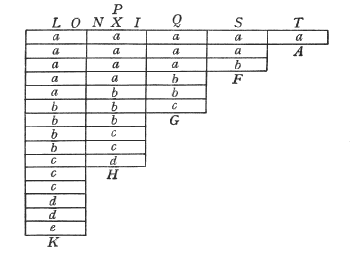
\includegraphics[width=8.75cm,height=6.35cm,keepaspectratio]{images/figura90.png} \end{center}
\end{center}

Sia la bilancia \emph{LT}; ad essa siano appese delle grandezze, tali quali abbiamo detto, e siano \emph{A}, \emph{F}, \emph{G}, \emph{H}, \emph{K}, la prima delle quali sia \emph{A}, appesa in \emph{T}. Dico che il centro di equilibrio interseca la bilancia \emph{TL} in modo che la parte verso \emph{T} è tripla dell'altra. Sia \emph{TL} tripla di \emph{LI}, \emph{SL} tripla di \emph{LP}, \emph{QL} lo sia di \emph{LN}, ed \emph{LP} di \emph{LO}: \emph{IP}, \emph{PN}, \emph{NO}, \emph{OL} risulteranno eguali. Si prenda in \emph{F} una grandezza doppia di \emph{A}, in \emph{G} se ne prenda un'altra tripla della medesima, in \emph{H} una quadrupla, e così via; le grandezze, che abbiamo prese, siano quelle segnate da \emph{a}. E si faccia lo stesso con le grandezze \emph{F}, \emph{G}, \emph{H}, \emph{K}: infatti, poiché in \emph{F} la grandezza rimanente, cioè \emph{b}, è eguale ad \emph{A}, in \emph{G} se ne prenda una doppia, in \emph{H} una tripla, ecc.; e queste grandezze prese siano quelle segnate da \emph{b}; e allo stesso modo si prendano le grandezze segnate da \emph{c}, e quelle segnate da \emph{d} e da \emph{e}. Tutte le grandezze segnate da \emph{a} [\emph{ossia la loro somma}] saranno allora eguali a \emph{K}; la grandezza composta da tutte le \emph{b} sarà eguale ad \emph{H}; quella composta dalle \emph{c}, sarà eguale a \emph{G}; quella composta da tutte le \emph{d}, sarà eguale ad \emph{F}; ed \emph{e} sarà eguale ad \emph{A}. Poiché \emph{TI} è doppia di \emph{IL}, \emph{I} sarà il punto dell'equilibrio della grandezza composta da tutte le \emph{a}; e, similmente, essendo \emph{SP} doppia di \emph{PL}, \emph{P} sarà il punto dell'equilibrio di quella composta da tutte le \emph{b}; e, per la stessa ragione, \emph{N} sarà il punto dell'equilibrio della grandezza composta da tutte le \emph{c}; \emph{O} lo sarà di quella composta dalle \emph{d}; ed \emph{L} [sarà il punto dell'equilibrio] della \emph{e}. Abbiamo dunque una bilancia \emph{TL}, alla quale sono appese ad eguali distanze alcune grandezze \emph{K}, \emph{H}, \emph{G}, \emph{F}, \emph{A}; e, inoltre, abbiamo un'altra bilancia \emph{LI}, sulla quale, a distanze similmente eguali, sono appese un altrettanto numero di grandezze, eguali alle predette e disposte nel medesimo ordine: infatti, la grandezza composta da tutte le \emph{a}, la quale è appesa in \emph{I}, è eguale alla grandezza \emph{K} appesa in \emph{L}; quella composta da tutte le \emph{b}, la quale è appesa in \emph{P}, è eguale alla \emph{H} appesa in \emph{P}; e, similmente, la grandezza composta dalle \emph{c}, la quale è appesa in \emph{N}, è eguale alla \emph{G}; quella composta dalle \emph{d}, la quale è appesa in \emph{O}, è eguale alla \emph{F}; e infine la \emph{e}, appesa in \emph{L}, è eguale alla \emph{A}. Perciò il centro del composto delle grandezze dividerà le bilance secondo la medesima proporzione: ma uno solo è il centro della grandezza composta dalle grandezze predette: esso sarà dunque un punto comune alla retta \emph{TL} e alla retta \emph{LI}; sia esso \emph{X}. Pertanto, come \emph{TX} sta a \emph{XL}, così \emph{LX} starà a \emph{XI}, e l'intera \emph{TL} starà ad \emph{LI}: ma \emph{TL} è tripla della \emph{LI}: perciò anche \emph{TX} sarà tripla della \emph{XL}.

Se si prendono un numero qualsiasi di grandezze in modo che la seconda sia superiore alla prima del triplo della prima, la terza sia superiore alla seconda del quintuplo della prima, la quarta sia superiore alla terza di sette volte la prima, e così di seguito l'aumento di ciascuna [grandezza] rispetto alla immediatamente precedente sia multiplo della prima grandezza secondo i numeri impari successivi, [cioè le grandezze] si succedano come i quadrati di linee egualmente eccedentisi l'una l'altra e il cui eccesso sia eguale alla minima; e se [tali grandezze] vengono appese a distanze eguali su una bilancia: il centro dell'equilibrio del composto di tutte [le grandezze] dividerà la bilancia in modo che la parte verso le grandezze minori risulterà maggiore del triplo dell'altra [parte], ma minore del triplo della medesima, qualora si tolga una distanza.


\begin{center}
\begin{center} 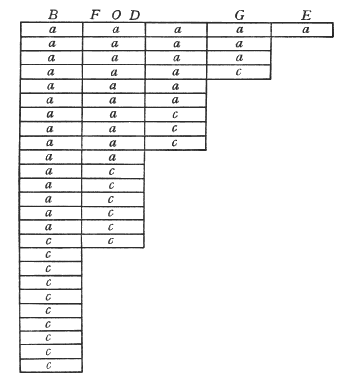
\includegraphics[width=8.75cm,height=9.55cm,keepaspectratio]{images/figura91.png} \end{center}
\end{center}

Sulla bilancia \emph{BE} siano delle grandezze, tali quali si è detto; dalle quali [immaginiamo che] ne vengano tolte alcune, le quali stiano tra di loro nella medesima proporzione in cui erano disposte le grandezze del [teorema] precedente; e siano quelle composte da tutte le \emph{a}; le altre, segnate da \emph{c}, saranno distribuite nel medesimo ordine, ma saranno prive della grandezza massima. \emph{ED} sia tripla di \emph{DB}, e \emph{GF} tripla di \emph{FB}; \emph{D} sarà il centro dell'equilibrio della grandezza composta da tutte le \emph{a}; \emph{F}, quello della grandezza composta da tutte le \emph{c}: perciò il centro della grandezza composta da tutte le \emph{a} e le \emph{c} andrà a cadere tra \emph{D} ed \emph{F}. Sia esso \emph{O}. È pertanto manifesto che \emph{EO} è più del triplo della \emph{OB}, mentre \emph{GO} è meno del triplo della \emph{OB}. Che è quello che si doveva dimostrare.

Se in un cono qualsiasi, o in una porzione di cono, si inscrive una figura [costituita] da cilindri aventi eguale altezza, e se ne circoscrive un'altra, e se, inoltre, l'asse del cono viene diviso in modo che la parte compresa tra il punto di divisione e il vertice sia tripla dell'altra; il centro di gravità della figura inscritta sarà più vicino del suddetto punto di divisione alla base del cono, mentre il centro di gravità della figura circoscritta sarà più vicino al vertice del medesimo punto.


\begin{center}
\begin{center} 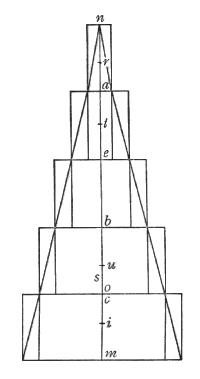
\includegraphics[width=5.00cm,height=9.47cm,keepaspectratio]{images/figura92.png} \end{center}
\end{center}

Sia dunque un cono, il cui asse \emph{nm} sia diviso in \emph{s} in modo che \emph{ns} sia tripla della rimanente \emph{sm}. Dico, che il centro di gravità di qualsiasi figura, inscritta al cono nel modo che si è detto, si trova sull'asse \emph{nm} ed è più vicino del punto \emph{s} alla base del cono; mentre il centro di gravità della figura circoscritta si trova similmente sull'asse \emph{nm}, ed e piu vicino di \emph{s} al vertice. Si intenda, pertanto, la figura inscritta [costituita] da cilindri, i cui assi \emph{mc}, \emph{cb}, \emph{be}, \emph{ea} siano eguali. Ordunque, il primo cilindro, il cui asse è \emph{mc}, rispetto al cilindro, il cui asse è \emph{cb}, ha la medesima proporzione che la sua base ha rispetto alla base dell'altro (infatti, le loro altezze sono eguali); ma questa proporzione è eguale a quella che il quadrato \emph{cn} ha al quadrato \emph{nb}. E similmente si mostrerà che il cilindro, il cui asse è \emph{cb}, rispetto al cilindro, il cui asse è \emph{be}, ha la medesima proporzione che il quadrato \emph{bn} ha rispetto al quadrato \emph{ne}; mentre il cilindro, il cui asse è \emph{be}, rispetto al cilindro, [che sta] intorno all'asse \emph{ea}, ha la medesima proporzione che il quadrato \emph{en} ha rispetto al quadrato \emph{na}. Ora, le linee \emph{nc}, \emph{nb}, \emph{en}, \emph{na} si eccedono egualmente tra di loro, e i loro eccessi sono eguali alla minima, cioè alla \emph{na}. Vi sono pertanto alcune grandezze, cioè i cilindri inscritti, tali che stanno tra di loro successivamente nella medesima proporzione in cui si trovano i quadrati di linee che si eccedono egualmente e i cui eccessi siano eguali alla minima: e [quei cilindri] sono disposti sulla bilancia \emph{ti} in modo che i loro singoli centri di gravità si trovino su di essa ad eguali distanze. Per le cose che si sono sopra dimostrate, risulta pertanto che il centro di gravità del composto di tutti [i cilindri] divide la bilancia \emph{ti} in modo che la parte verso \emph{t} sia più del triplo dell'altra. Sia \emph{o} questo centro; \emph{to}, dunque, è più che tripla della \emph{oi}. Ma \emph{tn} è tripla della \emph{im}; dunque, l'intera \emph{mo} sarà minore della quarta parte dell'intera \emph{mn}, della quale si è posta quarta parte la \emph{ms}. Ne risulta dunque che il punto \emph{o} è più vicino di \emph{s} alla base del cono. D'altra parte, sia poi circoscritta una figura costituita da cilindri, i cui assi \emph{mc}, \emph{cb}, \emph{be}, \emph{ea}, \emph{an} sono eguali tra loro. Similmente, come per i cilindri inscritti, si mostrerà che essi [cilindri circoscritti] stanno tra loro come i quadrati delle linee \emph{mn}, \emph{nc}, \emph{bn}, \emph{ne}, \emph{an}, le quali si eccedono egualmente e il cui eccesso è eguale alla minima \emph{an}; perciò, per la precedente [proposizione], il centro di gravità del composto di tutti i cilindri così disposti, il quale [centro] sia \emph{u}, divide la bilancia \emph{ri} in modo che la parte verso \emph{r}, cioè \emph{ru}, è più che tripla dell'altra [parte] \emph{ui}; \emph{tu}, invece, è minore del triplo della medesima. Ma \emph{nt} è tripla della \emph{im}; dunque, l'intera \emph{um} è maggiore della quarta parte dell'intera \emph{mn}, della quale si è posta quarta parte la \emph{ms}. Pertanto il punto \emph{u} è più vicino del punto \emph{s} al vertice. Che è quello che si doveva mostrare.

Dato un cono, è possibile circoscrivere ad esso una figura e inscrivergliene un'altra, [costituite] da cilindri aventi eguale altezza, in modo che la linea compresa tra il centro di gravità della figura circoscritta e il centro di gravità di quella inscritta, sia minore di qualsiasi linea assegnata.


\begin{center}
\begin{center} 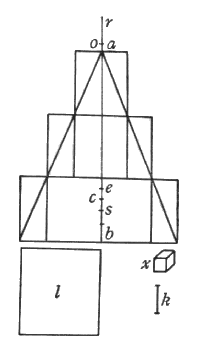
\includegraphics[width=5.00cm,height=8.75cm,keepaspectratio]{images/figura93.png} \end{center}
\end{center}

Sia dato un cono, il cui asse sia \emph{ab}; sia inoltre assegnata la retta \emph{k}. Dico: si ponga a parte il cilindro \emph{l}, eguale a quello che sia inscrivibile nel cono e abbia per altezza la metà dell'asse \emph{ab}; si divida poi \emph{ab} in \emph{c}, in modo che \emph{ac} sia tripla della \emph{cb}, e quale è la proporzione che \emph{ac} ha rispetto a \emph{k}, tale sia anche la proporzione che il cilindro \emph{l} ha rispetto al solido \emph{x}: si circoscriva poi al cono una figura [costituita] da cilindri aventi eguale altezza, e gli se ne inscriva un'altra, in modo che la figura circoscritta ecceda quella inscritta per una quantità minore del solido \emph{x}; il centro di gravità della figura circoscritta sia \emph{e}, il quale cadrà al di sopra di \emph{c}; il centro della figura inscritta sia, invece, \emph{s}, che cadrà al di sotto di \emph{c}. Dico allora che la linea \emph{es} è minore della \emph{k}. Infatti, qualora non lo fosse, si ponga \emph{eo} eguale alla \emph{ca}: pertanto, poiché \emph{oe} ha rispetto a \emph{k} la medesima proporzione che \emph{l} ha ad \emph{x}, poiché inoltre la figura inscritta non è minore del cilindro \emph{l}, mentre l'eccesso, per il quale tale figura è superata da quella circoscritta, è minore del solido \emph{x}: la figura inscritta avrà pertanto rispetto al suddetto eccesso una proporzione maggiore di quella che \emph{oe} ha rispetto a \emph{k}. Ma la proporzione di \emph{oe} a \emph{k} non è minore di quella di \emph{oe} ad \emph{es}, poiché \emph{es} non si pone minore di \emph{k}: pertanto la figura inscritta rispetto all'eccesso, per il quale è superata dalla figura circoscritta, ha una proporzione maggiore di quella di \emph{oe} ad \emph{es}. Quale è dunque la proporzione della figura inscritta al suddetto eccesso, tale sarà la proporzione che una linea maggiore della \emph{eo} ha rispetto alla linea \emph{es}. Sia essa \emph{er}; ora, il centro di gravità della figura inscritta è \emph{s}, mentre quello della figura circoscritta è \emph{e}: risulta, dunque, che il centro di gravità delle porzioni rimanenti, per le quali la figura circoscritta supera quella inscritta, si trova sulla linea \emph{re}, e proprio in quel punto, che la delimita in modo che, quale è la proporzione che la figura inscritta ha rispetto alle dette porzioni, tale sia anche la proporzione che la linea, compresa tra \emph{e} e quel punto, ha rispetto alla linea \emph{es}. Ma questa è la proporzione che \emph{re} ha ad \emph{es}; dunque, il centro di gravità delle rimanenti porzioni, per le quali la figura circoscritta supera quella inscritta, sarà \emph{r}: ciò che è impossibile; infatti il piano condotto per \emph{r} ed equidistante dalla base del cono non interseca le suddette porzioni. È pertanto falso che la linea \emph{es} non sia minore della \emph{k}; sarà dunque minore. Si dimostrerà poi, in modo analogo, che ciò è possibile anche per una piramide.

Da ciò è manifesto che a un cono dato è possibile circoscrivere una figura e inscriverne un'altra, [costituite] da cilindri aventi eguale altezza, in modo che le linee, le quali sono comprese tra i loro centri di gravità e il punto che divide l'asse del cono in modo che la parte verso il vertice è tripla dell'altra, siano minori di una qualunque linea data. Infatti, poiché, come si è dimostrato, il detto punto, che divide l'asse nel modo che si è detto, si trova sempre tra i centri di gravità della figura circoscritta e di quella inscritta; e poiché la linea, che è intermedia tra quei medesimi centri di gravità, può essere fatta minore di una qualsiasi linea assegnata; sarebbe molto minore della medesima linea assegnata quella linea che è compresa tra uno dei due centri e il suddetto punto che divide l'asse.

In qualsiasi cono o piramide il centro di gravità divide l'asse in modo che la parte verso il vertice è tripla della rimanente [parte] verso la base.


\begin{center}
\begin{center} 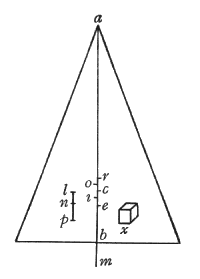
\includegraphics[width=5.00cm,height=6.98cm,keepaspectratio]{images/figura94.png} \end{center}
\end{center}

Sia un cono, il cui asse \emph{ab} sia diviso in \emph{c} in modo che \emph{ac} sia tripla della rimanente \emph{cb}: bisogna mostrare che \emph{c} è il centro di gravità del cono. Infatti, se non lo è, il centro del cono sarà o al di sopra o al di sotto del punto \emph{c}. In primo luogo [immaginiamo che] sia al di sotto, e sia \emph{e}; si ponga a parte la linea \emph{lp} eguale a \emph{ce}, e la si divida a caso in \emph{n}; e quale è la proporzione che [la somma di] ambedue le \emph{be} e \emph{pn} insieme ha rispetto a \emph{pn}, tale sia la proporzione che il cono ha al solido \emph{x}; si inscriva poi al cono una figura solida [costituita] da cilindri aventi eguale altezza, [figura] il cui centro di gravità si trovi a una distanza dal punto \emph{c} più breve della linea \emph{ln}; e l'eccesso, per il quale essa è superata dal cono, sia minore del solido \emph{x}. Che ciò sia possibile è, infatti, manifesto per le cose dimostrate. Sia allora inscritta, nel modo richiesto, la figura, il cui centro di gravità sia \emph{i}. Pertanto, la linea \emph{ie} sarà maggiore della \emph{np}, essendo \emph{lp} eguale a \emph{ce}; e \emph{ic} sarà minore di \emph{ln}: e poiché [la somma di] ambedue le \emph{be} ed \emph{np} sta ad \emph{np} come il cono sta a \emph{x}, mentre l'eccesso, per il quale il cono supera la figura inscritta, è minore del solido \emph{x}, dunque il cono avrà rispetto al suddetto eccesso una proporzione maggiore di quella che [la somma di] ambedue le \emph{be} ed \emph{np} ha ad \emph{np}; e, scomponendo, la figura inscritta avrà rispetto all'eccesso, per il quale essa è superata dal cono, una proporzione maggiore di quella che [\emph{be}] ha ad \emph{np}. Ma \emph{be} ha ad \emph{ei} una proporzione ancora minore di quella che \emph{be} ha ad \emph{np}, essendo \emph{ie} maggiore di \emph{np}; dunque, la figura inscritta avrà rispetto all'eccesso, per il quale è superata dal cono, una proporzione molto maggiore di quella che \emph{be} ha ad \emph{ei}. Pertanto, quale è la proporzione che la figura inscritta ha rispetto al suddetto eccesso, tale sarà la proporzione che rispetto ad \emph{ei} avrà una linea maggiore della \emph{be}. Sia essa \emph{me}: poiché, dunque, \emph{me} sta ad \emph{ei} come la figura inscritta sta all'eccesso, per il quale è superata dal cono, e poiché \emph{e} è il centro di gravità del cono, mentre \emph{i} è il centro di gravità della figura inscritta, sarà allora \emph{m} il centro di gravità delle porzioni rimanenti, per le quali il cono eccede la figura che gli è inscritta; ciò che è impossibile. Pertanto il centro di gravità del cono non si trova al di sotto del punto \emph{c}. Ma neppure [si troverà] sopra. Infatti, se è possibile, sia esso \emph{r}; e inoltre si prenda la linea \emph{lp}, divisa a caso in \emph{n}; e quale è la proporzione che [la somma di] ambedue le \emph{bc} ed \emph{np} ha ad \emph{nl}, tale sia la proporzione che il cono ha ad \emph{x}; e similmente si circoscriva al cono una figura, dalla quale esso sia superato per una quantità minore del solido \emph{x}; infine la linea, compresa tra il centro di gravità di quella [figura circoscritta] e \emph{c}, sia minore della \emph{np}. Sia, dunque, \emph{o} il centro di gravità della figura circoscritta: la rimanente \emph{or} sarà maggiore della \emph{nl}. E poiché, come [la somma di] ambedue le \emph{bc} e \emph{pn} sta ad \emph{nl}, così il cono sta a \emph{x}, mentre l'eccesso, per il quale il cono è superato dalla figura circoscritta, è minore di \emph{x}, e poiché la \emph{bo} è minore [della somma] di ambedue le \emph{bc} e \emph{pn}, mentre la \emph{or} è maggiore della \emph{ln}; il cono, dunque, rispetto alle rimanenti porzioni, per le quali è superato dalla figura circoscritta, avrà una proporzione molto maggiore di quella che \emph{bo} ha ad \emph{or}. Tale sia la proporzione di \emph{mo} a \emph{or}: \emph{mo} sarà maggiore di \emph{bc}; ed \emph{m} sarà il centro di gravità delle porzioni, per le quali il cono è superato dalla figura circoscritta; il che è sconveniente. Il centro di gravità del cono non si trova, dunque, al di sopra del punto \emph{c}: ma, come si è mostrato, neppure si trova al di sotto: dunque, esso sarà lo stesso \emph{c}. La stessa cosa, e con identico procedimento, si dimostrerà per una piramide qualsiasi.

\textbf{[LEMMA]}\\ Se si hanno quattro linee in proporzione continua; e se, quale è la proporzione che la minima di esse ha rispetto all'eccesso, per il quale la massima supera la minima, tale sia anche la proporzione che una linea [opportunamente] presa ha rispetto ai $\frac{3}{4}$ dell'eccesso, per il quale la massima supera la seconda; se, inoltre, quale è la proporzione che la linea eguale alla [somma della] massima, col doppio della seconda e col triplo della terza, ha rispetto alla linea eguale al [la somma del] quadruplo della massima, col quadruplo della seconda e col quadruplo della terza, tale sia la proporzione che un'altra linea [opportunamente] presa ha rispetto all'eccesso, per il quale la massima supera la seconda: queste due [ultime] linee, prese insieme [\emph{ossia la loro somma}], saranno la quarta parte della massima delle [linee] proporzionali [considerate].


\begin{center}
\begin{center} 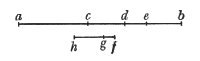
\includegraphics[width=5.00cm,height=1.53cm,keepaspectratio]{images/figura95.png} \end{center}
\end{center}

Siano infatti quattro linee proporzionali, \emph{ab}, \emph{bc}, \emph{bd}, \emph{be}; e quale è la proporzione che \emph{be} ha ad \emph{ea}, tale sia anche quella che \emph{fg} ha rispetto ai $\frac{3}{4}$ della \emph{ac}; inoltre, quale è la proporzione che la linea, eguale alla [somma di] \emph{ab}, col doppio di \emph{bc} e col triplo di \emph{bd}, ha rispetto alla linea, eguale al quadruplo [della somma] delle \emph{ab}, \emph{bc}, \emph{bd}, tale sia la proporzione che \emph{hg} ha ad \emph{ac}. Bisogna mostrare che \emph{hf} è la quarta parte della \emph{ab}. Pertanto, poiché le \emph{ab}, \emph{bc}, \emph{bd}, \emph{be} sono proporzionali, nella medesima proporzione si troveranno anche le \emph{ac}, \emph{cd}, \emph{de}; e come il quadruplo [della somma] delle \emph{ab}, \emph{bc}, \emph{bd} sta alla [somma di] \emph{ab} col doppio di \emph{bc} e col triplo di \emph{bd}, così il quadruplo [della somma] delle \emph{ac}, \emph{cd}, \emph{de}, cioè il quadruplo della \emph{ae}, sta alla [somma di] \emph{ac} col doppio di \emph{cd} e col triplo di \emph{de}; e così pure \emph{ac} sta ad \emph{hg}: dunque, come il triplo della \emph{ae} sta alla [somma di] \emph{ac} col doppio di \emph{cd} e col triplo di \emph{de}, così i $\frac{3}{4}$ della \emph{ac} stanno ad \emph{hg}. Ma come il triplo di \emph{ae} sta al triplo di \emph{eb}, così i $\frac{3}{4}$ della \emph{ac} stanno a \emph{gf}: dunque, per la reciproca della ventiquattresima del quinto, come il triplo della \emph{ae} sta alla [somma di] \emph{ac} col doppio di \emph{cd} e col triplo di \emph{db}, così i $\frac{3}{4}$ della \emph{ac} stanno ad \emph{hf}; e come il quadruplo della \emph{ae} sta alla [somma di] \emph{ac} col doppio di \emph{cd} e col triplo di \emph{db}, cioè alla [somma di] \emph{ab} con \emph{cb} e \emph{bd}, così \emph{ac} sta ad \emph{hf}; e, permutando, come il quadruplo di \emph{ae} sta ad \emph{ac}, così la [somma di] \emph{ab} con \emph{cb} e \emph{bd} sta ad \emph{hf}; ma come \emph{ac} sta ad \emph{ae}, così \emph{ab} sta alla [somma di] \emph{ab} con \emph{cb} e \emph{bd}: dunque, \emph{ex aequali}, in proporzione perturbata, come il quadruplo di \emph{ae} sta ad \emph{ae}, così \emph{ab} sta ad \emph{hf}. Risulta perciò che \emph{hf} è la quarta parte della \emph{ab}.

In un qualsiasi frusto di piramide, o di cono, intersecato da un piano equidistante dalla base, il centro di gravità si trova sull'asse, e lo si divide in modo che la parte verso la base minore sta alla [parte] rimanente come [la somma del] triplo della base maggiore col doppio dello spazio che è medio [proporzionale] tra la base maggiore e la minore, sta al [la somma del] triplo della base minore col doppio del medesimo spazio medio [proporzionale] e con la base maggiore.


\begin{center}
\begin{center} 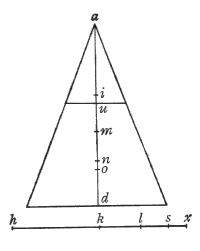
\includegraphics[width=5.00cm,height=6.28cm,keepaspectratio]{images/figura96.png} \end{center}
\end{center}

Dal cono o dalla piramide, il cui asse è \emph{ad}, per mezzo di un piano secante equidistante dalla base, sia staccato un frusto, il cui asse è \emph{ud}; e quale è la proporzione che [la somma del] triplo della base maggiore col doppio della media [proporzionale tra la base maggiore e la minore] e con la base minore, ha rispetto al [la somma del] triplo della base minore col doppio della media e con la massima, tale sia la proporzione che \emph{uo} ha ad \emph{od}. Bisogna mostrare che \emph{o} è il centro di gravità del frusto. Sia \emph{um} quarta parte della \emph{ud}. Si ponga a parte la linea \emph{hx} eguale alla \emph{ad}, e sia \emph{kx} eguale ad \emph{au}; inoltre delle \emph{hx} e \emph{kx} sia terza proporzionale \emph{xl}, e quarta proporzionale \emph{xs}: e quale è la proporzione che \emph{hs} ha ad \emph{sx}, tale sia quella che \emph{md} ha rispetto a una linea presa a partire da \emph{o} verso \emph{a}, la quale sia \emph{on}. E poiché la base maggiore sta a quella, che è media proporzionale tra la maggiore e la minore, come \emph{da} sta ad \emph{au}, cioè come \emph{hx} sta a \emph{xk}, mentre la detta media sta alla minore come \emph{kx} sta a \emph{xl}; la base maggiore, la media e la minore staranno tra di loro nella medesima proporzione [in cui stanno] anche le linee \emph{hx}, \emph{xk}, \emph{xl}. Perciò, come [la somma del] triplo della base maggiore col doppio della media e con la minore, sta al [la somma del] triplo della minima col doppio della media e con la massima, cioè come \emph{uo} sta a \emph{od}, così [la somma del] triplo di \emph{hx} col doppio di \emph{xk} e con \emph{xl}, sta al [la somma del] triplo di \emph{xl} col doppio di \emph{xk} e con \emph{xh}; e, componendo e permutando, \emph{od} starà a \emph{du}, come la [somma di] \emph{hx} col doppio di \emph{xk} e col triplo di \emph{xl} sta al quadruplo [della somma] delle \emph{hx}, \emph{xk}, \emph{xl}. Si hanno dunque quattro linee proporzionali, \emph{hx}, \emph{xk}, \emph{xl}, \emph{xs}; e quale è la proporzione che \emph{xs} ha ad \emph{sh}, tale è quella che una linea [opportunamente] presa \emph{no} ha rispetto ai $\frac{3}{4}$ della \emph{du}, cioè a \emph{dm}, cioè ai $\frac{3}{4}$ della \emph{hk}; inoltre, quale è la proporzione che la [somma di] \emph{hx} col doppio di \emph{xk} e col triplo di \emph{xl} ha rispetto al quadruplo [della somma] delle \emph{hx}, \emph{xk}, \emph{xl}, tale è anche la proporzione che un'altra linea [opportunamente] presa \emph{od} ha rispetto a \emph{du}, cioè ad \emph{hk}: dunque (per le cose che si sono dimostrate) \emph{dn} sarà la quarta parte della \emph{hx}, cioè della \emph{ad}; perciò il punto \emph{n} sarà il centro di gravità del cono, o della piramide, il cui asse è \emph{ad}. Sia \emph{i} il centro di gravità del cono, o della piramide, il cui asse è \emph{au}. Risulta, dunque, che il centro di gravità del frusto si trova sul prolungamento della linea \emph{in} dalla parte di \emph{n}, e proprio in quel punto che col punto \emph{n} delimita una linea tale, che rispetto ad essa \emph{in} abbia la medesima proporzione che il frusto staccato ha rispetto alla piramide o al cono, il cui asse è \emph{au}. Resta pertanto da mostrare che \emph{in} ha ad \emph{no} la medesima proporzione che il frusto ha rispetto al cono, il cui asse è \emph{au}. Ma come il cono, il cui asse è \emph{da}, sta al cono, il cui asse è \emph{au}, così il cubo \emph{da} sta al cubo \emph{au}, cioè il cubo \emph{hx} al cubo \emph{xk}: ma questa medesima proporzione è quella che \emph{hx} ha ad \emph{xs}: perciò, scomponendo, come \emph{hs} sta ad \emph{sx}, così il frusto, il cui asse è \emph{du}, starà al cono, o alla piramide, il cui asse è \emph{ua}. Ma come \emph{hs} sta ad \emph{sx}, così pure \emph{md} sta a \emph{on}; perciò il frusto sta alla piramide, il cui asse è \emph{au}, come \emph{md} sta ad \emph{no}. E poiché \emph{an} è $\frac{3}{4}$ della \emph{ad}, mentre \emph{ai} è $\frac{3}{4}$ della \emph{au}; la rimanente \emph{in} sarà 3/4 della rimanente \emph{ud}; perciò \emph{in} sarà eguale alla \emph{md}. Si è poi dimostrato che \emph{md} sta ad \emph{no} come il frusto sta al cono \emph{au}: risulta dunque che questa medesima proporzione è anche quella che \emph{in} ha ad \emph{no}. È perciò manifesto quello che ci eravamo proposti.

\end{document}
